\documentclass[11pt,a4paper]{article}
\usepackage[margin=22mm]{geometry}
\usepackage{fontspec}
\setmainfont{Latin Modern Roman}
\setsansfont{Latin Modern Sans}
\setmonofont{Latin Modern Mono}
\usepackage{amsmath,amssymb}
\usepackage{unicode-math}
\setmathfont{Latin Modern Math}
\usepackage{longtable,array,fvextra,adjustbox,needspace}
\usepackage{pgfplots}
\usepackage{pdflscape}
\pgfplotsset{compat=1.18}
\usepackage[colorlinks=true,linkcolor=blue,urlcolor=blue,unicode=true]{hyperref}
\usepackage{xurl}
\newcounter{listing}
\newcounter{scripttable}
\definecolor{pcd1}{HTML}{005A78}
\definecolor{pcd2}{HTML}{6B2CB1}
\definecolor{pcd3}{HTML}{447766}
\definecolor{pcd4}{HTML}{9A3E20}
\definecolor{pcd5}{HTML}{756000}
\setlength{\parindent}{0pt}
\setlength{\parskip}{0.65em}
\setlength{\emergencystretch}{3em}
\begin{document}
\hypersetup{pdftitle={Theoretical Distribution Models},pdfsubject={Authored thematic script},pdfcreator={Project Chemie Digital LaTeX exporter}}
\title{Theoretical Distribution Models}
\author{}
\date{}
\maketitle
\tableofcontents
\clearpage
\section{What a probability model describes}
Repeated measurements of the same homogeneous nitrate sample vary because injection, flow, temperature and electronics contribute to each result. The measurement path in \hyperref[material-66d09553c8dac37b41efc71c31ba53f9aeb75b651a92b6a99feeb480d8dd9293]{Fig.~\ref*{material-66d09553c8dac37b41efc71c31ba53f9aeb75b651a92b6a99feeb480d8dd9293}} makes that repeated experiment explicit. A probability model describes this variation under specified measurement conditions. The observed results form a finite sample from the population represented by that model.


\par\medskip
\Needspace{10cm}
\refstepcounter{figure}\label{material-66d09553c8dac37b41efc71c31ba53f9aeb75b651a92b6a99feeb480d8dd9293}
\noindent\textbf{Fig.~\ref*{material-66d09553c8dac37b41efc71c31ba53f9aeb75b651a92b6a99feeb480d8dd9293}.} One homogeneous nitrate control passes repeatedly through injection, separation, detection and reporting. The measurement path locates the contributions to variation.\par\nopagebreak
\begin{center}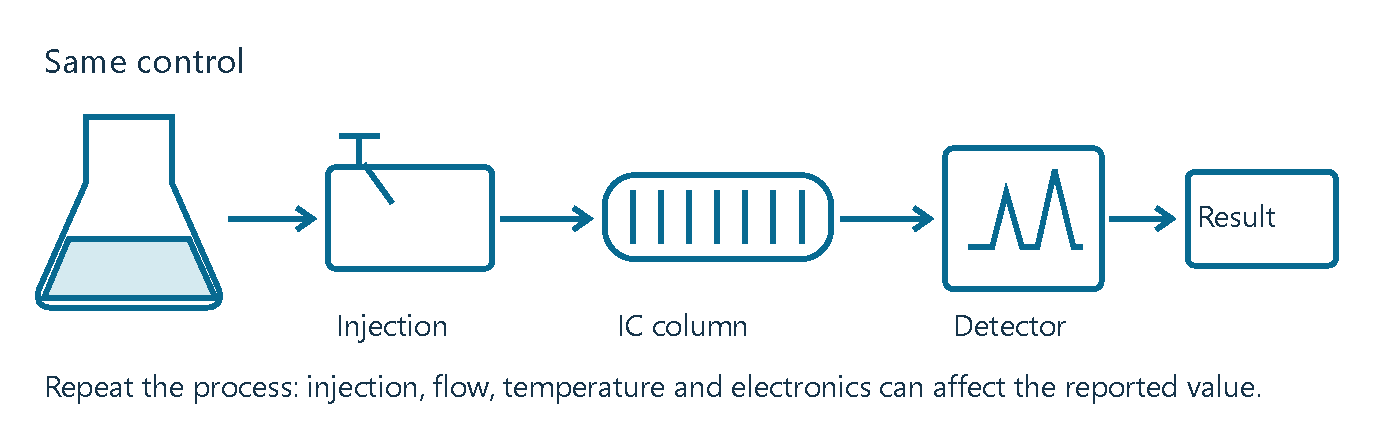
\includegraphics[width=\linewidth,height=.62\textheight,keepaspectratio]{asset-7a5def957ae76a94ae31679af4b0187b2e218c11279123eef4e9032988fd11f9.pdf}\end{center}

\medskip

Increasing sample size makes a generating distribution easier to recognize. It improves the empirical description of the population while the population's own standard deviation remains a property of the measurement model. The simulation in \hyperref[material-aa57516e19d13eced47e9a034d171e5fb696f150955f15c97de55dc780c9118d]{Fig.~\ref*{material-aa57516e19d13eced47e9a034d171e5fb696f150955f15c97de55dc780c9118d}} illustrates this distinction with successive samples from an unchanged method.


\par\medskip
\Needspace{10cm}
\refstepcounter{figure}\label{material-aa57516e19d13eced47e9a034d171e5fb696f150955f15c97de55dc780c9118d}
\noindent\textbf{Fig.~\ref*{material-aa57516e19d13eced47e9a034d171e5fb696f150955f15c97de55dc780c9118d}.} Successive prefixes of one simulated nitrate sequence: 20, 50, 100 and 1,000 results. All histograms use the same bin edges and Normal model with expectation 10.00 mg/L and SD 0.10 mg/L.\par\nopagebreak
\begin{center}
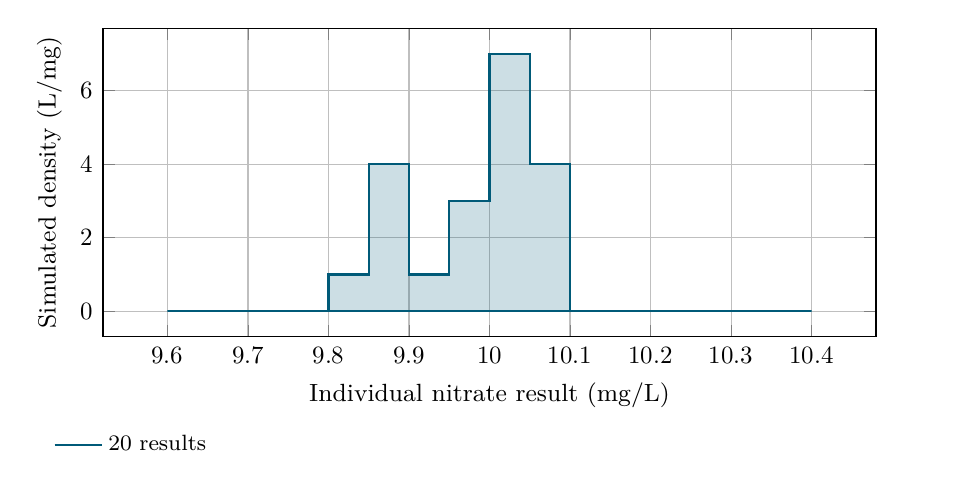
\begin{tikzpicture}
\begin{axis}[width=0.94\linewidth,
height=5.5cm,
scale only axis=false,
grid=major,
tick label style={font=\small},
label style={font=\small},
xlabel={Individual nitrate result (mg/L)},
ylabel={Simulated density (L/mg)},
legend style={font=\footnotesize,draw=none,at={(0.5,-0.28)},anchor=north,legend columns=1,text width=0.85\linewidth,align=left},
unbounded coords=jump,
scaled ticks=false]
\addplot[color=pcd1,thick,mark=none,fill=pcd1,fill opacity=0.2] coordinates {(9.6,0) (9.6,0) (9.65,0) (9.65,0) (9.7,0) (9.7,0) (9.75,0) (9.75,0) (9.8,0) (9.8,1.0000000000000213) (9.85,1.0000000000000213) (9.85,3.9999999999999436) (9.9,3.9999999999999436) (9.9,1.0000000000000213) (9.95,1.0000000000000213) (9.95,2.9999999999999574) (10,2.9999999999999574) (10,6.9999999999999005) (10.05,6.9999999999999005) (10.05,4.000000000000085) (10.1,4.000000000000085) (10.1,0) (10.15,0) (10.15,0) (10.2,0) (10.2,0) (10.25,0) (10.25,0) (10.3,0) (10.3,0) (10.35,0) (10.35,0) (10.4,0) (10.4,0)} \closedcycle;
\addlegendentry{20 results}

\end{axis}
\end{tikzpicture}
\end{center}
\noindent{\small\textit{The first 20 results from the same simulated sequence.}}\par

\begin{center}
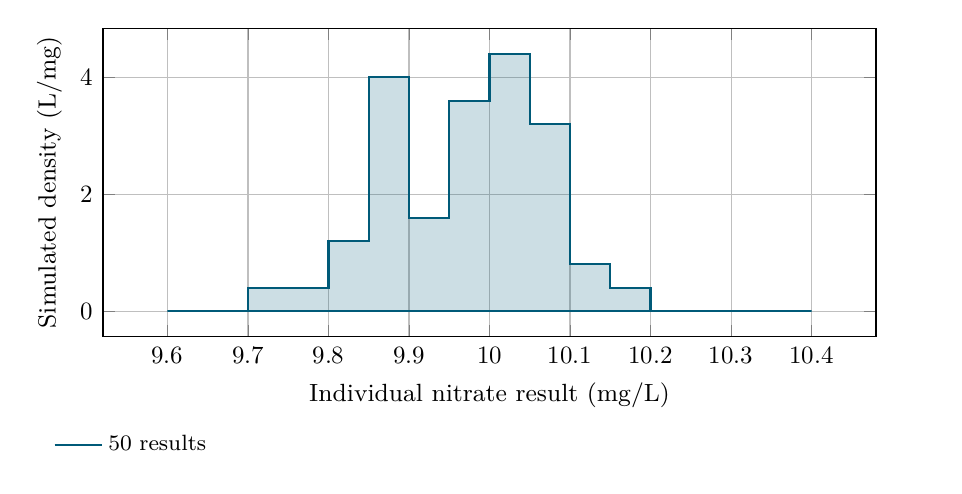
\begin{tikzpicture}
\begin{axis}[width=0.94\linewidth,
height=5.5cm,
scale only axis=false,
grid=major,
tick label style={font=\small},
label style={font=\small},
xlabel={Individual nitrate result (mg/L)},
ylabel={Simulated density (L/mg)},
legend style={font=\footnotesize,draw=none,at={(0.5,-0.28)},anchor=north,legend columns=1,text width=0.85\linewidth,align=left},
unbounded coords=jump,
scaled ticks=false]
\addplot[color=pcd1,thick,mark=none,fill=pcd1,fill opacity=0.2] coordinates {(9.6,0) (9.6,0) (9.65,0) (9.65,0) (9.7,0) (9.7,0.3999999999999943) (9.75,0.3999999999999943) (9.75,0.3999999999999943) (9.8,0.3999999999999943) (9.8,1.2000000000000255) (9.85,1.2000000000000255) (9.85,3.9999999999999436) (9.9,3.9999999999999436) (9.9,1.600000000000034) (9.95,1.600000000000034) (9.95,3.5999999999999486) (10,3.5999999999999486) (10,4.399999999999937) (10.05,4.399999999999937) (10.05,3.200000000000068) (10.1,3.200000000000068) (10.1,0.7999999999999886) (10.15,0.7999999999999886) (10.15,0.4000000000000085) (10.2,0.4000000000000085) (10.2,0) (10.25,0) (10.25,0) (10.3,0) (10.3,0) (10.35,0) (10.35,0) (10.4,0) (10.4,0)} \closedcycle;
\addlegendentry{50 results}

\end{axis}
\end{tikzpicture}
\end{center}
\noindent{\small\textit{The first 50 results from the same simulated sequence.}}\par

\begin{center}
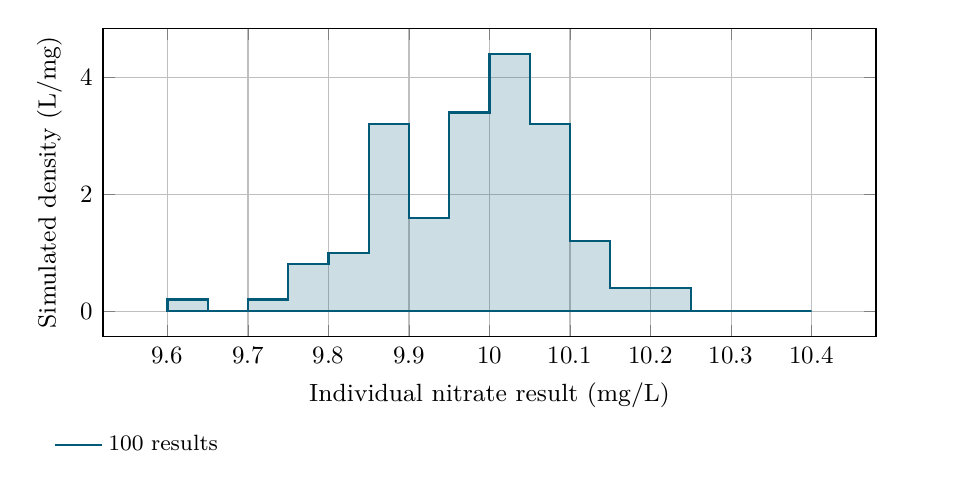
\begin{tikzpicture}
\begin{axis}[width=0.94\linewidth,
height=5.5cm,
scale only axis=false,
grid=major,
tick label style={font=\small},
label style={font=\small},
xlabel={Individual nitrate result (mg/L)},
ylabel={Simulated density (L/mg)},
legend style={font=\footnotesize,draw=none,at={(0.5,-0.28)},anchor=north,legend columns=1,text width=0.85\linewidth,align=left},
unbounded coords=jump,
scaled ticks=false]
\addplot[color=pcd1,thick,mark=none,fill=pcd1,fill opacity=0.2] coordinates {(9.6,0) (9.6,0.19999999999999715) (9.65,0.19999999999999715) (9.65,0) (9.7,0) (9.7,0.19999999999999715) (9.75,0.19999999999999715) (9.75,0.7999999999999886) (9.8,0.7999999999999886) (9.8,1.0000000000000213) (9.85,1.0000000000000213) (9.85,3.1999999999999544) (9.9,3.1999999999999544) (9.9,1.600000000000034) (9.95,1.600000000000034) (9.95,3.399999999999952) (10,3.399999999999952) (10,4.399999999999937) (10.05,4.399999999999937) (10.05,3.200000000000068) (10.1,3.200000000000068) (10.1,1.1999999999999829) (10.15,1.1999999999999829) (10.15,0.4000000000000085) (10.2,0.4000000000000085) (10.2,0.3999999999999943) (10.25,0.3999999999999943) (10.25,0) (10.3,0) (10.3,0) (10.35,0) (10.35,0) (10.4,0) (10.4,0)} \closedcycle;
\addlegendentry{100 results}

\end{axis}
\end{tikzpicture}
\end{center}
\noindent{\small\textit{The first 100 results from the same simulated sequence.}}\par

\begin{center}
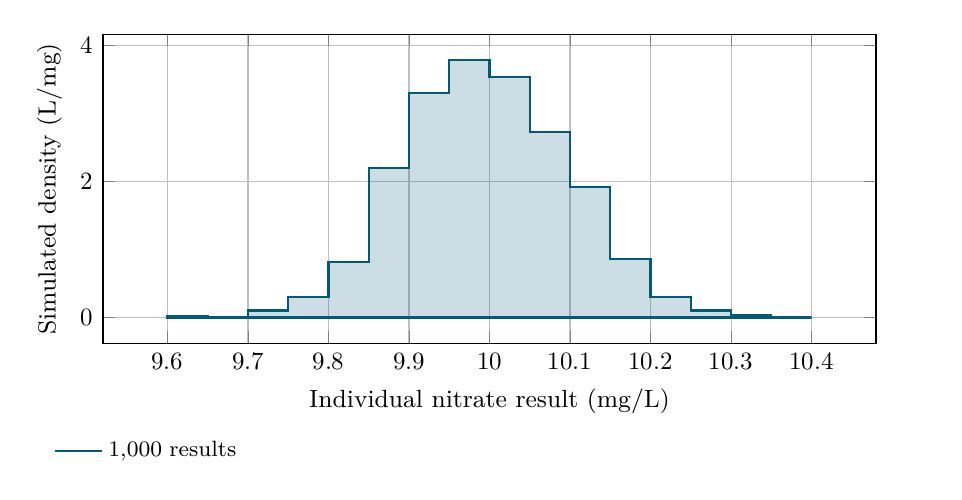
\begin{tikzpicture}
\begin{axis}[width=0.94\linewidth,
height=5.5cm,
scale only axis=false,
grid=major,
tick label style={font=\small},
label style={font=\small},
xlabel={Individual nitrate result (mg/L)},
ylabel={Simulated density (L/mg)},
legend style={font=\footnotesize,draw=none,at={(0.5,-0.28)},anchor=north,legend columns=1,text width=0.85\linewidth,align=left},
unbounded coords=jump,
scaled ticks=false]
\addplot[color=pcd1,thick,mark=none,fill=pcd1,fill opacity=0.2] coordinates {(9.6,0) (9.6,0.019999999999999716) (9.65,0.019999999999999716) (9.65,0) (9.7,0) (9.7,0.09999999999999858) (9.75,0.09999999999999858) (9.75,0.2999999999999957) (9.8,0.2999999999999957) (9.8,0.8200000000000175) (9.85,0.8200000000000175) (9.85,2.1999999999999686) (9.9,2.1999999999999686) (9.9,3.3000000000000704) (9.95,3.3000000000000704) (9.95,3.7799999999999465) (10,3.7799999999999465) (10,3.5399999999999494) (10.05,3.5399999999999494) (10.05,2.7200000000000584) (10.1,2.7200000000000584) (10.1,1.9199999999999728) (10.15,1.9199999999999728) (10.15,0.8600000000000183) (10.2,0.8600000000000183) (10.2,0.2999999999999957) (10.25,0.2999999999999957) (10.25,0.09999999999999858) (10.3,0.09999999999999858) (10.3,0.040000000000000854) (10.35,0.040000000000000854) (10.35,0) (10.4,0) (10.4,0)} \closedcycle;
\addlegendentry{1,000 results}

\end{axis}
\end{tikzpicture}
\end{center}
\noindent{\small\textit{The first 1,000 results from the same simulated sequence.}}\par

\medskip

A model becomes useful when it answers a specified analytical question. We may want the probability that a result falls within an interval, the probability below a concentration limit, or the limit corresponding to a chosen probability. Each calculation starts by identifying the random quantity, its population or measurement conditions, and the assumptions behind its distribution. Individual injections, sample means and concentrations from environmental sites each have their own sampling context.


The optional R source in \hyperref[material-6cf5c7917d6715bee57478c8ffefd926ea0b73bd7225c19e0796fc01c5394265]{Listing~\ref*{material-6cf5c7917d6715bee57478c8ffefd926ea0b73bd7225c19e0796fc01c5394265}} makes the simulation reproducible. The following chapters develop the analytical questions from common probability tools to particular distribution families. The simulated examples illustrate consequences of the stated models. Assessing a laboratory method's model additionally draws on observations from the measurement process and the conditions under which they were collected.


\par\medskip
\Needspace{8\baselineskip}
\refstepcounter{listing}\label{material-6cf5c7917d6715bee57478c8ffefd926ea0b73bd7225c19e0796fc01c5394265}
\noindent\textbf{Listing~\ref*{material-6cf5c7917d6715bee57478c8ffefd926ea0b73bd7225c19e0796fc01c5394265}.} R reproduction of the fixed-seed nitrate simulation and its histogram prefixes.\par\nopagebreak
\begin{Verbatim}[fontsize=\footnotesize,breaklines=true,breakanywhere=true]
# Assumed normal generator, not fitted or measured validation data.
M <- 20 # Try 20, 50, 100, 1000. The browser uses these saved prefixes.
stopifnot(M %in% c(20,50,100,1000))
state <- 20261102; x <- numeric(M)
for(i in seq_len(M)) {
  state <- (16807 * state) %% 2147483647
  x[i] <- 10 + .10 * qnorm(state/2147483647)
}
edges <- seq(9.60,10.40,by=.05)
h <- hist(x,breaks=edges,right=FALSE,plot=FALSE)
cat('M:',M,'counted:',sum(h$counts),'\n')
cat('Counts:',h$counts,'\n')
plot(h,freq=FALSE,col='#8ecae6',xlab='Nitrate result (mg/L)',
     ylab='Simulated density (L/mg)',main='Assumed stable normal generator')

\end{Verbatim}

\par\noindent\textbf{R functions and the deterministic stream}

\begin{itemize}\setlength{\itemsep}{1pt}\setlength{\parsep}{0pt}
\item \textbf{Choose the sample size.} \texttt{c} lists the allowed result counts. \texttt{\%in\%} checks whether \texttt{M} belongs to that list, and \texttt{stopifnot} enforces this choice.
\item \textbf{Prepare the simulation.} \texttt{numeric} allocates the result vector; \texttt{seq\_len} supplies the iteration indices.
\item \textbf{Generate reproducible results.} The Park–Miller recurrence updates an integer-valued state using multiplication and the remainder operator \texttt{\%\%}. \texttt{qnorm} transforms the resulting uniform fractions into standard-normal values. Scaling and shifting set the stated SD and mean.
\item \textbf{Build the histogram.} \texttt{seq} creates fixed bin edges. \texttt{hist} computes and draws density bins whose left edges belong to the bin.
\item \textbf{Check the counts.} \texttt{sum} totals the bin counts; \texttt{cat} reports that total alongside \texttt{M} so that count conservation can be checked.
\end{itemize}

\medskip

\clearpage
\section{From density areas to cumulative probabilities and quantiles}
Once a probability model has been specified, we can ask how likely an individual result is to fall within a chosen concentration interval. For a model with a probability density, the answer depends on both the curve's height and the interval's width. A high, narrow region can contain less probability than a lower, wider region. The area combines height and width into the probability for the complete interval.


Integrating the density over the interval calculates this area. In the nitrate example, concentration is measured in mg/L and density in L/mg; multiplying density by a concentration increment gives a dimensionless probability. Each exact concentration has zero point probability in this continuous model. A rounded laboratory report represents a concentration interval at the stated measurement resolution.


The observed fraction of simulated results inside an interval summarizes the finite sample. Its variation from run to run shows how sampling affects the empirical result. Comparing this fraction with the density area connects the observed sample with its generating model (\hyperref[material-375b546a8169ea8db13585f9fdb4e2d9889c10d2cff01ca16673ce7aa1c3767d]{Fig.~\ref*{material-375b546a8169ea8db13585f9fdb4e2d9889c10d2cff01ca16673ce7aa1c3767d}}). The ECDF in \hyperref[material-098f71e548c0b7552806f3915c4b08aeecc95511a7badff0f06893614572d313]{Fig.~\ref*{material-098f71e548c0b7552806f3915c4b08aeecc95511a7badff0f06893614572d313}} makes the distinction between a finite sample and a smooth population model visible on the cumulative scale.


\par\medskip
\Needspace{10cm}
\refstepcounter{figure}\label{material-375b546a8169ea8db13585f9fdb4e2d9889c10d2cff01ca16673ce7aa1c3767d}
\noindent\textbf{Fig.~\ref*{material-375b546a8169ea8db13585f9fdb4e2d9889c10d2cff01ca16673ce7aa1c3767d}.} A histogram of 1,000 simulated nitrate results and its generating Normal density share concentration axes. Between 9.9 and 10.1 mg/L, the observed sample fraction is 66.7\%, compared with a model probability of about 68.27\%.\par\nopagebreak
\begin{center}
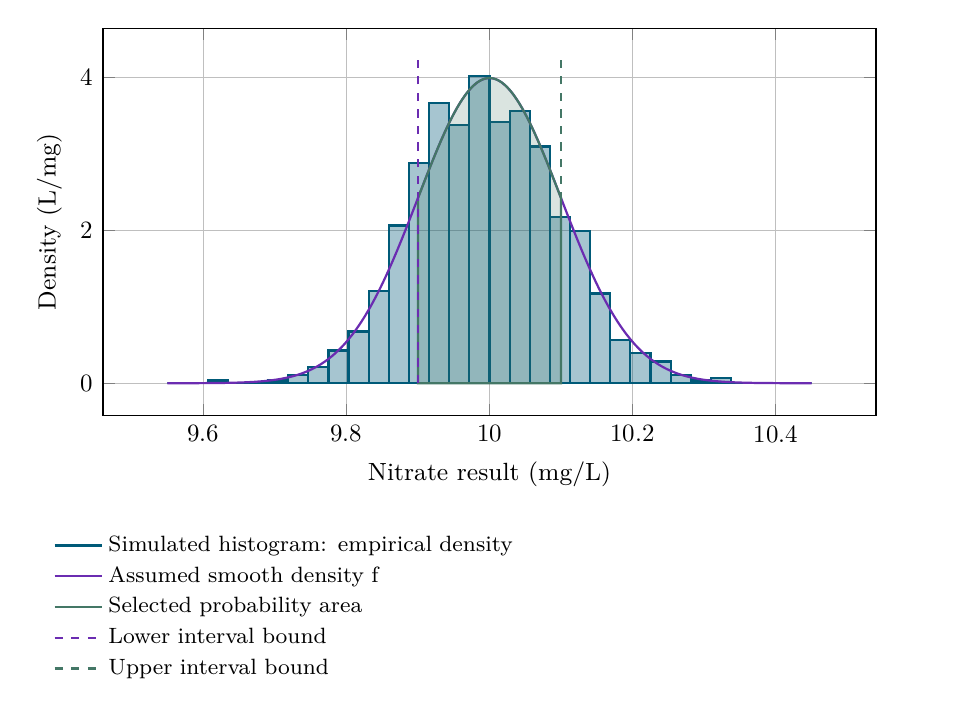
\begin{tikzpicture}
\begin{axis}[width=0.94\linewidth,
height=6.5cm,
scale only axis=false,
grid=major,
tick label style={font=\small},
label style={font=\small},
xlabel={Nitrate result (mg/L)},
ylabel={Density (L/mg)},
legend style={font=\footnotesize,draw=none,at={(0.5,-0.28)},anchor=north,legend columns=1,text width=0.85\linewidth,align=left},
unbounded coords=jump,
scaled ticks=false]
\addplot[color=pcd1,thick,fill=pcd1,fill opacity=0.35,mark=none] coordinates {(9.55,0) (9.55,0) (9.578125,0) (9.578125,0)} \closedcycle;
\addplot[color=pcd1,thick,fill=pcd1,fill opacity=0.35,forget plot,mark=none] coordinates {(9.578125,0) (9.578125,0) (9.606250000000003,0) (9.606250000000003,0)} \closedcycle;
\addplot[color=pcd1,thick,fill=pcd1,fill opacity=0.35,forget plot,mark=none] coordinates {(9.60625,0) (9.60625,0.03555555555555561) (9.634375000000002,0.03555555555555561) (9.634375000000002,0)} \closedcycle;
\addplot[color=pcd1,thick,fill=pcd1,fill opacity=0.35,forget plot,mark=none] coordinates {(9.634374999999999,0) (9.634374999999999,0) (9.662500000000001,0) (9.662500000000001,0)} \closedcycle;
\addplot[color=pcd1,thick,fill=pcd1,fill opacity=0.35,forget plot,mark=none] coordinates {(9.662500000000001,0) (9.662500000000001,0) (9.690625,0) (9.690625,0)} \closedcycle;
\addplot[color=pcd1,thick,fill=pcd1,fill opacity=0.35,forget plot,mark=none] coordinates {(9.690625,0) (9.690625,0.03555555555555561) (9.71875,0.03555555555555561) (9.71875,0)} \closedcycle;
\addplot[color=pcd1,thick,fill=pcd1,fill opacity=0.35,forget plot,mark=none] coordinates {(9.71875,0) (9.71875,0.10666666666666684) (9.746875,0.10666666666666684) (9.746875,0)} \closedcycle;
\addplot[color=pcd1,thick,fill=pcd1,fill opacity=0.35,forget plot,mark=none] coordinates {(9.746875,0) (9.746875,0.21333333333333368) (9.775000000000002,0.21333333333333368) (9.775000000000002,0)} \closedcycle;
\addplot[color=pcd1,thick,fill=pcd1,fill opacity=0.35,forget plot,mark=none] coordinates {(9.774999999999999,0) (9.774999999999999,0.42666666666666736) (9.803125000000001,0.42666666666666736) (9.803125000000001,0)} \closedcycle;
\addplot[color=pcd1,thick,fill=pcd1,fill opacity=0.35,forget plot,mark=none] coordinates {(9.803125000000001,0) (9.803125000000001,0.6755555555555566) (9.83125,0.6755555555555566) (9.83125,0)} \closedcycle;
\addplot[color=pcd1,thick,fill=pcd1,fill opacity=0.35,forget plot,mark=none] coordinates {(9.83125,0) (9.83125,1.208888888888891) (9.859375,1.208888888888891) (9.859375,0)} \closedcycle;
\addplot[color=pcd1,thick,fill=pcd1,fill opacity=0.35,forget plot,mark=none] coordinates {(9.859375,0) (9.859375,2.0622222222222257) (9.8875,2.0622222222222257) (9.8875,0)} \closedcycle;
\addplot[color=pcd1,thick,fill=pcd1,fill opacity=0.35,forget plot,mark=none] coordinates {(9.8875,0) (9.8875,2.880000000000005) (9.915625000000002,2.880000000000005) (9.915625000000002,0)} \closedcycle;
\addplot[color=pcd1,thick,fill=pcd1,fill opacity=0.35,forget plot,mark=none] coordinates {(9.915624999999999,0) (9.915624999999999,3.6622222222222276) (9.943750000000001,3.6622222222222276) (9.943750000000001,0)} \closedcycle;
\addplot[color=pcd1,thick,fill=pcd1,fill opacity=0.35,forget plot,mark=none] coordinates {(9.943749999999998,0) (9.943749999999998,3.377777777777783) (9.971875,3.377777777777783) (9.971875,0)} \closedcycle;
\addplot[color=pcd1,thick,fill=pcd1,fill opacity=0.35,forget plot,mark=none] coordinates {(9.971875,0) (9.971875,4.017777777777784) (10,4.017777777777784) (10,0)} \closedcycle;
\addplot[color=pcd1,thick,fill=pcd1,fill opacity=0.35,forget plot,mark=none] coordinates {(10,0) (10,3.413333333333339) (10.028125,3.413333333333339) (10.028125,0)} \closedcycle;
\addplot[color=pcd1,thick,fill=pcd1,fill opacity=0.35,forget plot,mark=none] coordinates {(10.028125,0) (10.028125,3.5555555555555616) (10.056250000000002,3.5555555555555616) (10.056250000000002,0)} \closedcycle;
\addplot[color=pcd1,thick,fill=pcd1,fill opacity=0.35,forget plot,mark=none] coordinates {(10.056249999999999,0) (10.056249999999999,3.093333333333338) (10.084375000000001,3.093333333333338) (10.084375000000001,0)} \closedcycle;
\addplot[color=pcd1,thick,fill=pcd1,fill opacity=0.35,forget plot,mark=none] coordinates {(10.084374999999998,0) (10.084374999999998,2.168888888888892) (10.1125,2.168888888888892) (10.1125,0)} \closedcycle;
\addplot[color=pcd1,thick,fill=pcd1,fill opacity=0.35,forget plot,mark=none] coordinates {(10.1125,0) (10.1125,1.9911111111111144) (10.140625,1.9911111111111144) (10.140625,0)} \closedcycle;
\addplot[color=pcd1,thick,fill=pcd1,fill opacity=0.35,forget plot,mark=none] coordinates {(10.140625,0) (10.140625,1.1733333333333353) (10.16875,1.1733333333333353) (10.16875,0)} \closedcycle;
\addplot[color=pcd1,thick,fill=pcd1,fill opacity=0.35,forget plot,mark=none] coordinates {(10.16875,0) (10.16875,0.5688888888888898) (10.196874999999999,0.5688888888888898) (10.196874999999999,0)} \closedcycle;
\addplot[color=pcd1,thick,fill=pcd1,fill opacity=0.35,forget plot,mark=none] coordinates {(10.196874999999999,0) (10.196874999999999,0.3911111111111117) (10.225000000000001,0.3911111111111117) (10.225000000000001,0)} \closedcycle;
\addplot[color=pcd1,thick,fill=pcd1,fill opacity=0.35,forget plot,mark=none] coordinates {(10.224999999999998,0) (10.224999999999998,0.2844444444444449) (10.253125,0.2844444444444449) (10.253125,0)} \closedcycle;
\addplot[color=pcd1,thick,fill=pcd1,fill opacity=0.35,forget plot,mark=none] coordinates {(10.253125,0) (10.253125,0.10666666666666684) (10.28125,0.10666666666666684) (10.28125,0)} \closedcycle;
\addplot[color=pcd1,thick,fill=pcd1,fill opacity=0.35,forget plot,mark=none] coordinates {(10.28125,0) (10.28125,0.03555555555555561) (10.309375,0.03555555555555561) (10.309375,0)} \closedcycle;
\addplot[color=pcd1,thick,fill=pcd1,fill opacity=0.35,forget plot,mark=none] coordinates {(10.309375,0) (10.309375,0.07111111111111122) (10.337499999999999,0.07111111111111122) (10.337499999999999,0)} \closedcycle;
\addplot[color=pcd1,thick,fill=pcd1,fill opacity=0.35,forget plot,mark=none] coordinates {(10.337499999999999,0) (10.337499999999999,0) (10.365625000000001,0) (10.365625000000001,0)} \closedcycle;
\addplot[color=pcd1,thick,fill=pcd1,fill opacity=0.35,forget plot,mark=none] coordinates {(10.365624999999998,0) (10.365624999999998,0) (10.39375,0) (10.39375,0)} \closedcycle;
\addplot[color=pcd1,thick,fill=pcd1,fill opacity=0.35,forget plot,mark=none] coordinates {(10.393749999999997,0) (10.393749999999997,0) (10.421875,0) (10.421875,0)} \closedcycle;
\addplot[color=pcd1,thick,fill=pcd1,fill opacity=0.35,forget plot,mark=none] coordinates {(10.421875,0) (10.421875,0) (10.45,0) (10.45,0)} \closedcycle;
\addlegendentry{Simulated histogram: empirical density}
\addplot[color=pcd2,thick,mark=none] coordinates {(9.55,0.00015983741106905986) (9.555625000000001,0.00020555221443492518) (9.561250000000001,0.00026350675221400733) (9.566875000000001,0.000336734180265155) (9.572500000000002,0.00042895182550130095) (9.578125,0.0005446979040605383) (9.58375,0.0006894912403168897) (9.589375,0.0008700168562871747) (9.595,0.0010943404343980345) (9.600625,0.001372154740440402) (9.606250000000001,0.0017150611119473064) (9.611875000000001,0.002136889052371542) (9.6175,0.002654056803802257) (9.623125,0.003285975479652018) (9.62875,0.0040554989019461595) (9.634375,0.004989420683443525) (9.64,0.00611901930113785) (9.645625,0.007480650904521929) (9.651250000000001,0.009116388371642704) (9.656875000000001,0.011074703654578032) (9.662500000000001,0.013411188734904421) (9.668125,0.01618930853714581) (9.67375,0.019481176930604863) (9.679375,0.0233683445037857) (9.685,0.027942584148794893) (9.690625,0.0333066576862686) (9.696250000000001,0.0395750438493009) (9.701875000000001,0.04687460499686597) (9.7075,0.05534516702780428) (9.713125,0.06513998421484826) (9.71875,0.07642605818746402) (9.724375,0.0893842781881537) (9.73,0.10420934814422717) (9.735625,0.12110946517803635) (9.74125,0.14030571406719194) (9.746875000000001,0.16203114300393665) (9.752500000000001,0.18652948792270502) (9.758125,0.21405351578525703) (9.76375,0.2448629616303991) (9.769375,0.27922203997788564) (9.775,0.31739651835667665) (9.780625,0.35965034929518336) (9.78625,0.40624186700824017) (9.791875000000001,0.4574195661301623) (9.7975,0.5134174920076886) (9.803125,0.5744502850548727) (9.80875,0.6407079351997078) (9.814375,0.7123503161825093) (9.82,0.7895015830089458) (9.825625,0.8722445287894649) (9.83125,0.960615009051145) (9.836875000000001,1.054596551912006) (9.842500000000001,1.1541152807835204) (9.848125,1.2590352820521005) (9.85375,1.3691545530567721) (9.859375,1.4842016652517789) (9.865,1.6038332734192007) (9.870625,1.7276325939605182) (9.87625,1.8551089635442763) (9.881875,1.9856985737288606) (9.8875,2.118766457756978) (9.893125,2.253609782807206) (9.89875,2.3894624749971483) (9.904375,2.5255011759069204) (9.91,2.660852498987552) (9.915625,2.794601522708553) (9.92125,2.925801425530651) (9.926875,3.0534841366761056) (9.932500000000001,3.1766718471515034) (9.938125,3.2943891984970586) (9.94375,3.4056759431983) (9.949375,3.5095998514368985) (9.955,3.605269624616481) (9.960625,3.691847567477099) (9.96625,3.7685617680601826) (9.971875,3.834717538569453) (9.9775,3.889707880367487) (9.983125,3.9330227528236015) (9.98875,3.964256948154329) (9.994375,3.983116402246566) (10,3.989422804014327) (10.005625,3.983116402246566) (10.01125,3.964256948154329) (10.016875,3.9330227528236015) (10.0225,3.889707880367487) (10.028125,3.834717538569453) (10.03375,3.7685617680601826) (10.039375,3.691847567477099) (10.045,3.605269624616481) (10.050625,3.5095998514368985) (10.05625,3.4056759431983) (10.061875,3.2943891984970586) (10.067499999999999,3.1766718471515034) (10.073125,3.0534841366761056) (10.07875,2.925801425530651) (10.084375,2.794601522708553) (10.09,2.660852498987552) (10.095625,2.5255011759069204) (10.10125,2.3894624749971483) (10.106875,2.253609782807206) (10.1125,2.118766457756978) (10.118125,1.9856985737288606) (10.12375,1.8551089635442763) (10.129375,1.7276325939605182) (10.135,1.6038332734192007) (10.140625,1.4842016652517789) (10.14625,1.3691545530567721) (10.151875,1.2590352820521005) (10.157499999999999,1.1541152807835204) (10.163124999999999,1.054596551912006) (10.16875,0.960615009051145) (10.174375,0.8722445287894649) (10.18,0.7895015830089458) (10.185625,0.7123503161825093) (10.19125,0.6407079351997078) (10.196875,0.5744502850548727) (10.2025,0.5134174920076886) (10.208124999999999,0.4574195661301623) (10.21375,0.40624186700824017) (10.219375,0.35965034929518336) (10.225,0.31739651835667665) (10.230625,0.27922203997788564) (10.23625,0.2448629616303991) (10.241875,0.21405351578525703) (10.247499999999999,0.18652948792270502) (10.253124999999999,0.16203114300393665) (10.25875,0.14030571406719194) (10.264375,0.12110946517803635) (10.27,0.10420934814422717) (10.275625,0.0893842781881537) (10.28125,0.07642605818746402) (10.286875,0.06513998421484826) (10.2925,0.05534516702780428) (10.298124999999999,0.04687460499686597) (10.303749999999999,0.0395750438493009) (10.309375,0.0333066576862686) (10.315,0.027942584148794893) (10.320625,0.0233683445037857) (10.32625,0.019481176930604863) (10.331875,0.01618930853714581) (10.337499999999999,0.013411188734904421) (10.343124999999999,0.011074703654578032) (10.348749999999999,0.009116388371642704) (10.354375,0.007480650904521929) (10.36,0.00611901930113785) (10.365625,0.004989420683443525) (10.37125,0.0040554989019461595) (10.376875,0.003285975479652018) (10.3825,0.002654056803802257) (10.388124999999999,0.002136889052371542) (10.393749999999999,0.0017150611119473064) (10.399375,0.001372154740440402) (10.405,0.0010943404343980345) (10.410625,0.0008700168562871747) (10.41625,0.0006894912403168897) (10.421875,0.0005446979040605383) (10.427499999999998,0.00042895182550130095) (10.433124999999999,0.000336734180265155) (10.438749999999999,0.00026350675221400733) (10.444374999999999,0.00020555221443492518) (10.45,0.00015983741106905986)};
\addlegendentry{Assumed smooth density f}
\addplot[color=pcd3,thick,mark=none,fill=pcd3,fill opacity=0.2] coordinates {(9.9,2.419707245191442) (9.901250000000001,2.4499520055403323) (9.9025,2.4801872461073677) (9.90375,2.5104033433347377) (9.905000000000001,2.540590564691918) (9.90625,2.5707390734673474) (9.9075,2.600838933699972) (9.90875,2.630880115247252) (9.91,2.660852498987552) (9.91125,2.6907458821522954) (9.9125,2.7205499837854266) (9.91375,2.750254450326049) (9.915000000000001,2.7798488613099863) (9.91625,2.8093227351869765) (9.9175,2.838665535248883) (9.918750000000001,2.8678666756641693) (9.92,2.896915527614826) (9.92125,2.925801425530651) (9.9225,2.954513673415616) (9.92375,2.9830415512623096) (9.925,3.01137432154806) (9.92625,3.039501235808458) (9.9275,3.0674115412824046) (9.92875,3.095094487622759) (9.93,3.1225393336676066) (9.93125,3.149735354265941) (9.932500000000001,3.1766718471515034) (9.93375,3.203338139859422) (9.935,3.2297235966791535) (9.93625,3.2558176256371354) (9.9375,3.2816096855037507) (9.93875,3.3070892928170905) (9.94,3.3322460289179867) (9.94125,3.357069546989378) (9.9425,3.3815495790931296) (9.94375,3.4056759431983) (9.945,3.4294385501938445) (9.946250000000001,3.452827410878748) (9.9475,3.4758326429234767) (9.94875,3.498444477795666) (9.95,3.5206532676429823) (9.95125,3.5424494921272096) (9.9525,3.563823765201842) (9.95375,3.5847668418272653) (9.955,3.605269624616481) (9.95625,3.6253231704044633) (9.9575,3.644918696735058) (9.95875,3.66404758825856) (9.96,3.682701403033246) (9.96125,3.7008718787248944) (9.9625,3.7185509386976943) (9.963750000000001,3.7357306979900193) (9.965,3.7524034691693773) (9.96625,3.7685617680601826) (9.9675,3.7841983193381865) (9.96875,3.7993060619862775) (9.97,3.8138781546052485) (9.97125,3.827907980574508) (9.9725,3.841389153057049) (9.97375,3.854315519843218) (9.975,3.8666811680284887) (9.97625,3.878480428520087) (9.977500000000001,3.8897078803675025) (9.97875,3.900358354912579) (9.98,3.9104269397545623) (9.98125,3.9199089825257136) (9.9825,3.9288000944737926) (9.98375,3.9370961538471136) (9.985,3.944793309078886) (9.98625,3.9518879817672183) (9.9875,3.9583768694474983) (9.98875,3.964256948154329) (9.99,3.969525474770119) (9.99125,3.9741799891577245) (9.9925,3.9782183160749707) (9.99375,3.981638566868867) (9.995,3.9844391409476385) (9.99625,3.9866187270290934) (9.9975,3.9881763041638183) (9.99875,3.9891111425321983) (10,3.989422804014327) (10.00125,3.9891111425321983) (10.0025,3.9881763041638183) (10.00375,3.9866187270290934) (10.005,3.9844391409476385) (10.00625,3.981638566868867) (10.0075,3.9782183160749707) (10.00875,3.9741799891577245) (10.01,3.969525474770119) (10.01125,3.964256948154329) (10.0125,3.9583768694474983) (10.01375,3.9518879817672183) (10.015,3.944793309078886) (10.01625,3.9370961538471136) (10.0175,3.9288000944737926) (10.01875,3.9199089825257136) (10.02,3.9104269397545623) (10.02125,3.900358354912579) (10.022499999999999,3.8897078803675025) (10.02375,3.878480428520087) (10.025,3.8666811680284887) (10.02625,3.854315519843218) (10.0275,3.841389153057049) (10.02875,3.827907980574508) (10.03,3.8138781546052485) (10.03125,3.7993060619862775) (10.0325,3.7841983193381865) (10.03375,3.7685617680601826) (10.035,3.7524034691693773) (10.036249999999999,3.7357306979900193) (10.0375,3.7185509386976943) (10.03875,3.7008718787248944) (10.04,3.682701403033246) (10.04125,3.66404758825856) (10.0425,3.644918696735058) (10.04375,3.6253231704044633) (10.045,3.605269624616481) (10.04625,3.5847668418272653) (10.0475,3.563823765201842) (10.04875,3.5424494921272096) (10.05,3.5206532676429823) (10.05125,3.498444477795666) (10.0525,3.4758326429234767) (10.053749999999999,3.452827410878748) (10.055,3.4294385501938445) (10.05625,3.4056759431983) (10.0575,3.3815495790931296) (10.05875,3.357069546989378) (10.06,3.3322460289179867) (10.06125,3.3070892928170905) (10.0625,3.2816096855037507) (10.06375,3.2558176256371354) (10.065,3.2297235966791535) (10.06625,3.203338139859422) (10.067499999999999,3.1766718471515034) (10.06875,3.149735354265941) (10.07,3.1225393336676066) (10.07125,3.095094487622759) (10.0725,3.0674115412824046) (10.07375,3.039501235808458) (10.075,3.01137432154806) (10.07625,2.9830415512623096) (10.0775,2.954513673415616) (10.07875,2.925801425530651) (10.08,2.896915527614826) (10.081249999999999,2.8678666756641693) (10.0825,2.838665535248883) (10.08375,2.8093227351869765) (10.084999999999999,2.7798488613099863) (10.08625,2.750254450326049) (10.0875,2.7205499837854266) (10.08875,2.6907458821522954) (10.09,2.660852498987552) (10.09125,2.630880115247252) (10.0925,2.600838933699972) (10.09375,2.5707390734673474) (10.094999999999999,2.540590564691918) (10.09625,2.5104033433347377) (10.0975,2.4801872461073677) (10.098749999999999,2.4499520055403323) (10.1,2.419707245191442)} \closedcycle;
\addlegendentry{Selected probability area}
\addplot[color=pcd2,dashed,thick] coordinates {(9.9,0) (9.9,4.218666666666674)};
\addlegendentry{Lower interval bound}
\addplot[color=pcd3,dashed,thick] coordinates {(10.1,0) (10.1,4.218666666666674)};
\addlegendentry{Upper interval bound}
\end{axis}
\end{tikzpicture}
\end{center}

% Full-precision experiment details: {"blockId":"ex:pc-n09-v--block","parameters":[{"key":"location","label":"Assumed model expectation (mg/L)","value":10},{"key":"scale","label":"Assumed model SD (mg/L)","value":0.1},{"key":"threshold","label":"Interval center (mg/L)","value":10},{"key":"width","label":"Interval half-width (mg/L)","value":0.1},{"key":"probability","label":"Quantile question reserved for the next scene","value":0.95},{"key":"family","label":"Model: 0 smooth bell, 1 bounded flat","value":0},{"key":"M","label":"Fixed reference replay count","value":1000},{"key":"seed","label":"Fixed reference replay seed","value":20261102},{"key":"view","label":"Histogram and interval area","value":0}],"readouts":[{"label":"Simulated results","value":1000},{"label":"Lower bound (mg/L)","value":9.9},{"label":"Upper bound (mg/L)","value":10.1},{"label":"Model interval probability","value":0.6826894921370847},{"label":"Empirical interval fraction","value":0.667}],"note":"Histogram bars describe the finite simulated sample; f describes its generating model. The selected interval area gives the model probability. Its observed sample fraction varies between simulated samples.","markers":[[{"x":9.9,"label":"Lower interval bound"},{"x":10.1,"label":"Upper interval bound"}]]}

\medskip

\par\medskip
\Needspace{10cm}
\refstepcounter{figure}\label{material-098f71e548c0b7552806f3915c4b08aeecc95511a7badff0f06893614572d313}
\noindent\textbf{Fig.~\ref*{material-098f71e548c0b7552806f3915c4b08aeecc95511a7badff0f06893614572d313}.} The empirical CDF of 20 simulated nitrate results is compared with the generating Normal CDF. All 20 observations lie at or below 10.20 mg/L, giving empirical fraction 1 at that threshold; the model probability there is about 97.72\%. Steps accumulate observed fractions, while the smooth curve accumulates model probability.\par\nopagebreak
\begin{center}
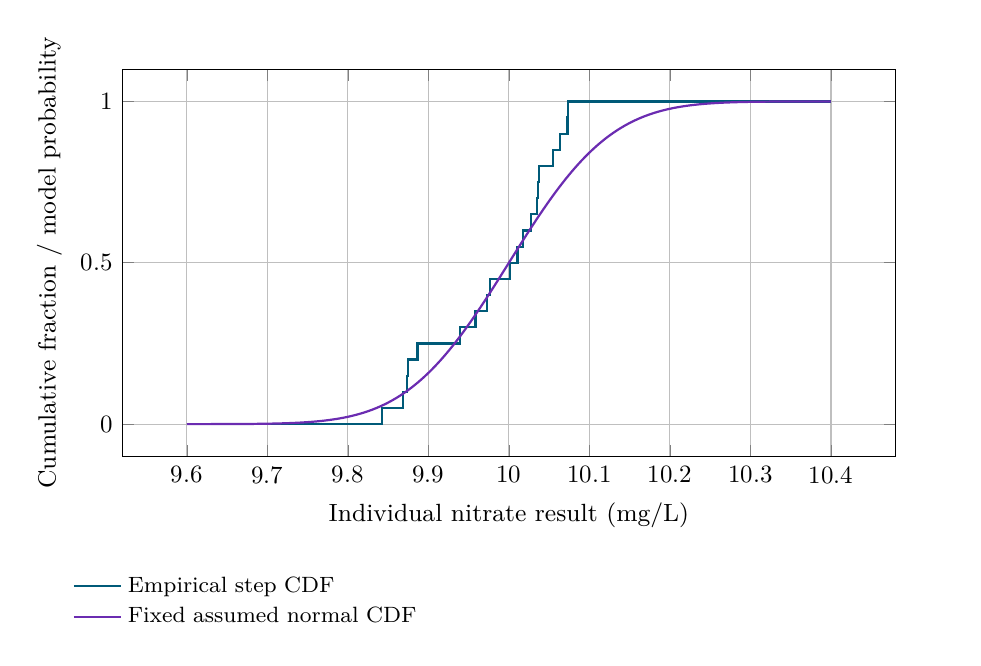
\begin{tikzpicture}
\begin{axis}[width=0.94\linewidth,
height=6.5cm,
scale only axis=false,
grid=major,
tick label style={font=\small},
label style={font=\small},
xlabel={Individual nitrate result (mg/L)},
ylabel={Cumulative fraction / model probability},
legend style={font=\footnotesize,draw=none,at={(0.5,-0.28)},anchor=north,legend columns=1,text width=0.85\linewidth,align=left},
unbounded coords=jump,
scaled ticks=false]
\addplot[color=pcd1,thick,mark=none] coordinates {(9.6,0) (9.84260730574354,0) (9.84260730574354,0.05) (9.868905858317811,0.05) (9.868905858317811,0.1) (9.873721091636407,0.1) (9.873721091636407,0.15) (9.874761311915965,0.15) (9.874761311915965,0.2) (9.886422887285226,0.2) (9.886422887285226,0.25) (9.939524268863446,0.25) (9.939524268863446,0.3) (9.958607953166783,0.3) (9.958607953166783,0.35) (9.972659718619624,0.35) (9.972659718619624,0.4) (9.976738565613736,0.4) (9.976738565613736,0.45) (10.00118727535754,0.45) (10.00118727535754,0.5) (10.010654010619579,0.5) (10.010654010619579,0.55) (10.017857899331974,0.55) (10.017857899331974,0.6) (10.02749984945395,0.6) (10.02749984945395,0.65) (10.034791487053077,0.65) (10.034791487053077,0.7) (10.036039441787487,0.7) (10.036039441787487,0.75) (10.037611271477676,0.75) (10.037611271477676,0.8) (10.055114816949695,0.8) (10.055114816949695,0.85) (10.063118143902578,0.85) (10.063118143902578,0.9) (10.072863982500582,0.9) (10.072863982500582,0.95) (10.073120346268695,0.95) (10.073120346268695,1) (10.4,1)};
\addlegendentry{Empirical step CDF}
\addplot[color=pcd2,thick,mark=none] coordinates {(9.6,0.00003167124183311946) (9.605,0.00003907559659778821) (9.61,0.00004809634401760163) (9.615,0.000059058912418923045) (9.62,0.00007234804392511773) (9.625,0.00008841728520080392) (9.629999999999999,0.00010779973347738408) (9.635,0.00013112015442048346) (9.64,0.00015910859015753738) (9.645,0.00019261557563562972) (9.65,0.00023262907903552813) (9.655,0.0002802932768161706) (9.66,0.00033692926567688313) (9.665,0.00040405780186400877) (9.67,0.00048342414238377614) (9.674999999999999,0.000577025042390746) (9.68,0.0006871379379158416) (9.685,0.000816352312828576) (9.69,0.0009676032132183394) (9.695,0.0011442068310227112) (9.7,0.0013498980316300636) (9.705,0.0015888696473648723) (9.709999999999999,0.0018658133003839814) (9.715,0.0021859614549132314) (9.719999999999999,0.0025551303304278397) (9.725,0.0029797632350545217) (9.73,0.003466973803040703) (9.735,0.004024588542758233) (9.74,0.004661188023718774) (9.745,0.005386145954066566) (9.75,0.006209665325776127) (9.754999999999999,0.007142810735271214) (9.76,0.00819753592459605) (9.765,0.0093867055348387) (9.77,0.010724110021675667) (9.775,0.012224472655044796) (9.78,0.013903447513498363) (9.785,0.015777607391090544) (9.79,0.01786442056281616) (9.795,0.02018221540570432) (9.8,0.02275013194817947) (9.805,0.02558805952163841) (9.81,0.028716559816002043) (9.815,0.032156774795613186) (9.82,0.03593031911292592) (9.825,0.04005915686381632) (9.83,0.044565462758542784) (9.834999999999999,0.04947146803364688) (9.84,0.05479929169955772) (9.845,0.06057075800205958) (9.85,0.06680720126885753) (9.855,0.07352925960964873) (9.86,0.08075665923377001) (9.865,0.08850799143740218) (9.87,0.09680048458560869) (9.875,0.10564977366685507) (9.879999999999999,0.115069670221706) (9.885,0.1250719356371497) (9.89,0.13566606094638378) (9.895,0.1468590563758948) (9.9,0.15865525393145768) (9.905,0.17105612630848016) (9.91,0.1840601253467598) (9.915,0.19766254312268977) (9.92,0.2118553985833963) (9.925,0.22662735237687015) (9.93,0.24196365222307198) (9.935,0.2578461108058663) (9.94,0.2742531177500718) (9.945,0.29115968678834725) (9.95,0.30853753872598433) (9.955,0.32635522028792013) (9.96,0.3445782583896789) (9.965,0.36316934882438034) (9.97,0.38208857781104977) (9.975,0.4012936743170749) (9.98,0.42074029056089857) (9.985,0.4403823076297552) (9.99,0.46017216272297184) (9.995,0.4800611941616244) (10,0.5) (10.005,0.5199388058383756) (10.01,0.5398278372770282) (10.015,0.5596176923702447) (10.02,0.5792597094391014) (10.025,0.598706325682925) (10.03,0.6179114221889502) (10.035,0.6368306511756197) (10.04,0.6554217416103211) (10.045,0.6736447797120799) (10.05,0.6914624612740157) (10.055,0.7088403132116528) (10.06,0.7257468822499282) (10.065,0.7421538891941337) (10.07,0.7580363477769281) (10.075,0.7733726476231298) (10.08,0.7881446014166037) (10.085,0.8023374568773103) (10.09,0.8159398746532402) (10.095,0.8289438736915198) (10.1,0.8413447460685424) (10.105,0.8531409436241052) (10.11,0.8643339390536162) (10.115,0.8749280643628503) (10.120000000000001,0.884930329778294) (10.125,0.8943502263331449) (10.13,0.9031995154143913) (10.135,0.9114920085625978) (10.14,0.9192433407662299) (10.145,0.9264707403903513) (10.15,0.9331927987311425) (10.155,0.9394292419979404) (10.16,0.9452007083004423) (10.165000000000001,0.9505285319663531) (10.17,0.9554345372414572) (10.175,0.9599408431361837) (10.18,0.9640696808870741) (10.185,0.9678432252043868) (10.19,0.9712834401839979) (10.195,0.9744119404783615) (10.2,0.9772498680518206) (10.205,0.9798177845942957) (10.21,0.9821355794371839) (10.215,0.9842223926089094) (10.22,0.9860965524865016) (10.225,0.9877755273449552) (10.23,0.9892758899783244) (10.235,0.9906132944651613) (10.24,0.991802464075404) (10.245000000000001,0.9928571892647288) (10.25,0.9937903346742238) (10.255,0.9946138540459334) (10.26,0.9953388119762813) (10.265,0.9959754114572418) (10.27,0.9965330261969593) (10.275,0.9970202367649454) (10.280000000000001,0.9974448696695721) (10.285,0.9978140385450868) (10.290000000000001,0.9981341866996161) (10.295,0.9984111303526352) (10.3,0.9986501019683699) (10.305,0.9988557931689773) (10.31,0.9990323967867817) (10.315,0.9991836476871714) (10.32,0.9993128620620841) (10.325000000000001,0.9994229749576092) (10.33,0.9995165758576162) (10.335,0.999595942198136) (10.34,0.9996630707343231) (10.345,0.9997197067231838) (10.35,0.9997673709209645) (10.355,0.9998073844243643) (10.36,0.9998408914098424) (10.365,0.9998688798455795) (10.370000000000001,0.9998922002665226) (10.375,0.9999115827147992) (10.38,0.9999276519560749) (10.385,0.999940941087581) (10.39,0.9999519036559824) (10.395,0.9999609244034022) (10.4,0.9999683287581669)};
\addlegendentry{Fixed assumed normal CDF}

\end{axis}
\end{tikzpicture}
\end{center}

% Full-precision experiment details: {"blockId":"ex:rv-n16-v--block","parameters":[{"key":"sigma","label":"True method SD (mg/L), assumed","value":0.1},{"key":"mu","label":"Assumed method expectation (mg/L)","value":10},{"key":"threshold","label":"Chosen threshold (mg/L)","value":10.2},{"key":"M","label":"Results in the seeded prefix","value":20},{"key":"seed","label":"Replay seed (Park-Miller)","value":20261102}],"readouts":[{"label":"Results in same seeded prefix","value":20},{"label":"Empirical fraction at threshold","value":1},{"label":"Full-model probability at threshold","value":0.9772498680518206},{"label":"Threshold (mg/L)","value":10.2},{"label":"Observed count at threshold","value":"20/20"}],"note":"The empirical curve includes observations equal to the threshold. Increasing the prefix length adds results from the same generating model and reveals how observed sample fractions compare with its CDF.","markers":[[]]}

\medskip

Many analytical questions concern everything at or below a limit. The cumulative distribution function, or CDF, answers that question directly. For a model with a density, its value at a threshold is the area accumulated up to that threshold. The PDF and CDF describe the same model, but their vertical axes mean different things: density height in the PDF and accumulated probability in the CDF. The probability between two bounds is consequently the upper CDF value minus the lower one.


Where density is high, accumulated probability increases rapidly and the CDF rises steeply. Where the derivative relation holds, the CDF's slope equals the density. Every distribution has a CDF. For absolutely continuous models, accumulated probability can be expressed as density area; for discrete distributions, probability masses produce jumps. An empirical CDF accumulates observed sample fractions in steps.


We can now reverse the threshold question: choose a cumulative probability and seek its corresponding concentration. A model quantile supplies this threshold. In the continuous Normal and bounded uniform examples, the 0.95 quantile leaves 95\% of the model probability at or below it. The observed fraction below that fixed threshold varies between finite samples.


More generally, a quantile is the lowest threshold at which the CDF reaches or exceeds the chosen probability. At a probability jump, the accumulated probability can exceed the requested value. This construction is the generalized inverse of the CDF. Density, CDF and quantile are complementary descriptions: integrate over an interval, accumulate up to a threshold, or find a threshold for a chosen accumulated probability.


The interval identity in \hyperref[material-8c205665b2843f7b93de1bd2386075765078a7c40dccc71a1b4c2ccfa996307d]{Eq.~\ref*{material-8c205665b2843f7b93de1bd2386075765078a7c40dccc71a1b4c2ccfa996307d}} and the function relationships in \hyperref[material-c13dcb3e4886b0cd0c5b37d6baf085db10d1d0fa29ea54ad6b36e6f005cf61d1]{Eq.~\ref*{material-c13dcb3e4886b0cd0c5b37d6baf085db10d1d0fa29ea54ad6b36e6f005cf61d1}} provide equivalent tools for choosing limits. Their equivalence also has a graphical interpretation (\hyperref[material-26632d678ea06aced51987cbb6bb1c6ba0a7b6b7ed82132516137c5e4b2c0046]{Fig.~\ref*{material-26632d678ea06aced51987cbb6bb1c6ba0a7b6b7ed82132516137c5e4b2c0046}}). Reversing the calculation gives a model-based concentration limit for a prescribed upper-tail rate (\hyperref[material-d5d05efcdd8a06801dd5a158b8891a5dc14f41a3402fa3fbb5c37dc23548257b]{Eq.~\ref*{material-d5d05efcdd8a06801dd5a158b8891a5dc14f41a3402fa3fbb5c37dc23548257b}}). Finite-sample fractions vary around their fixed model probabilities; the optional R example in \hyperref[material-9c0e8d6352f7ca3835e957a15da673db61154f61b7ffec37dda6c8bd12221b02]{Listing~\ref*{material-9c0e8d6352f7ca3835e957a15da673db61154f61b7ffec37dda6c8bd12221b02}} allows this sampling variation to be explored.


\par\medskip
\noindent\begin{minipage}{\linewidth}
\refstepcounter{equation}\label{material-8c205665b2843f7b93de1bd2386075765078a7c40dccc71a1b4c2ccfa996307d}
\noindent\textbf{Eq.~\ref*{material-8c205665b2843f7b93de1bd2386075765078a7c40dccc71a1b4c2ccfa996307d}.} Interval probability as an area under the model density.\par\nopagebreak
\begin{center}\begin{adjustbox}{max width=\linewidth}$\displaystyle P(a\le X\le b)=\int_a^b f(x)\,dx=F(b)-F(a)$\end{adjustbox}\end{center}

\par\noindent\textbf{Symbols}

\begin{itemize}\setlength{\itemsep}{1pt}\setlength{\parsep}{0pt}
\item \textbf{X}: Random individual nitrate concentration (mg/L).
\item \textbf{x}: Concrete concentration coordinate (mg/L).
\item \textbf{a, b}: Ordered lower and upper interval bounds (mg/L).
\item \textbf{P}: Probability of the stated event (dimensionless).
\item \textbf{f(x)}: Model probability density at x (L/mg).
\item \textbf{F(x)}: Cumulative probability at or below x (dimensionless).
\item \textbf{\ensuremath{\int}, dx}: Accumulate density over the interval; dx is an infinitesimal concentration increment (mg/L).
\item \textbf{\ensuremath{\le}}: Includes the interval endpoints, each with zero point probability.
\item \textbf{=, \ensuremath{-}}: Equality between equivalent probabilities; subtraction of the lower CDF value from the upper.
\end{itemize}

The density is nonnegative and has total area one. Integrating density times concentration gives a dimensionless probability.

\end{minipage}\par
\medskip

\par\medskip
\noindent\begin{minipage}{\linewidth}
\refstepcounter{equation}\label{material-c13dcb3e4886b0cd0c5b37d6baf085db10d1d0fa29ea54ad6b36e6f005cf61d1}
\noindent\textbf{Eq.~\ref*{material-c13dcb3e4886b0cd0c5b37d6baf085db10d1d0fa29ea54ad6b36e6f005cf61d1}.} Density, cumulative probability and the generalized quantile function.\par\nopagebreak
\begin{center}\begin{adjustbox}{max width=\linewidth}$\displaystyle \begin{gathered}F(x)=P(X\le x)=\int_{-\infty}^{x}f(t)\,dt\\f(x)=F'(x)\quad\text{where the derivative exists}\\x_p=F^{-1}(p)\end{gathered}$\end{adjustbox}\end{center}

\par\noindent\textbf{Symbols}

\begin{itemize}\setlength{\itemsep}{1pt}\setlength{\parsep}{0pt}
\item \textbf{X}: Random concentration (mg/L).
\item \textbf{x}: Concrete concentration threshold (mg/L).
\item \textbf{F(x)}: Cumulative probability at or below x (dimensionless).
\item \textbf{P, \ensuremath{\le}}: Probability of an event; at or below the threshold.
\item \textbf{f(t)}: Probability density at concentration t (L/mg).
\item \textbf{t, dt}: Integration coordinate and its infinitesimal increment (mg/L).
\item \textbf{\ensuremath{\int}, \ensuremath{-}\ensuremath{\infty}}: Integrate up to x over an unbounded lower range.
\item \textbf{F\ensuremath{\prime}(x)}: Derivative of F with respect to x; the local slope (L/mg).
\item \textbf{=}: Equality linking the expressions.
\end{itemize}

Conditions: the integral representation uses an absolutely continuous model. The slope equals f where the derivative relation holds. Every distribution has a CDF; existence of a PDF requires additional conditions.

\begin{itemize}\setlength{\itemsep}{1pt}\setlength{\parsep}{0pt}
\item \textbf{p}: Chosen cumulative probability, strictly between zero and one.
\item \textbf{\(x_p\)}: Concentration quantile at probability \(p\) (mg/L); subscript \(p\) identifies the probability.
\item \textbf{F\ensuremath{{}^-}\ensuremath{{}^1}(p)}: Quantile function, the generalized inverse CDF evaluated at p.
\end{itemize}

The generalized inverse is the greatest lower bound of thresholds whose cumulative probability is at least \(p\). For continuous, strictly increasing \(F\), it is the usual inverse function. In these continuous examples, \(p = 0.95\) places 95\% probability at or below \(x_p\).

\end{minipage}\par
\medskip

\par\medskip
\Needspace{10cm}
\refstepcounter{figure}\label{material-26632d678ea06aced51987cbb6bb1c6ba0a7b6b7ed82132516137c5e4b2c0046}
\noindent\textbf{Fig.~\ref*{material-26632d678ea06aced51987cbb6bb1c6ba0a7b6b7ed82132516137c5e4b2c0046}.} The density panel's shaded area and the CDF panel's marked height represent the same accumulated probability, about 84.13\%. Both panels use a concentration threshold of 10.1 mg/L under the Normal model with expectation 10.00 mg/L and SD 0.10 mg/L. The model's 95\% quantile is about 10.16 mg/L.\par\nopagebreak
\begin{center}
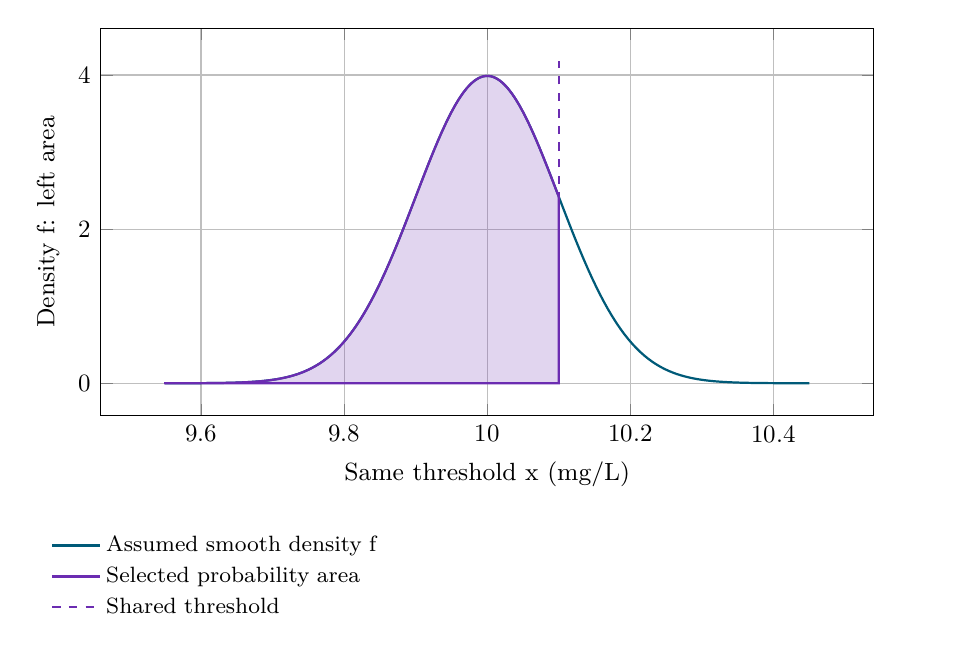
\begin{tikzpicture}
\begin{axis}[width=0.94\linewidth,
height=6.5cm,
scale only axis=false,
grid=major,
tick label style={font=\small},
label style={font=\small},
xlabel={Same threshold x (mg/L)},
ylabel={Density f: left area},
legend style={font=\footnotesize,draw=none,at={(0.5,-0.28)},anchor=north,legend columns=1,text width=0.85\linewidth,align=left},
unbounded coords=jump,
scaled ticks=false]
\addplot[color=pcd1,thick,mark=none] coordinates {(9.55,0.00015983741106905986) (9.555625000000001,0.00020555221443492518) (9.561250000000001,0.00026350675221400733) (9.566875000000001,0.000336734180265155) (9.572500000000002,0.00042895182550130095) (9.578125,0.0005446979040605383) (9.58375,0.0006894912403168897) (9.589375,0.0008700168562871747) (9.595,0.0010943404343980345) (9.600625,0.001372154740440402) (9.606250000000001,0.0017150611119473064) (9.611875000000001,0.002136889052371542) (9.6175,0.002654056803802257) (9.623125,0.003285975479652018) (9.62875,0.0040554989019461595) (9.634375,0.004989420683443525) (9.64,0.00611901930113785) (9.645625,0.007480650904521929) (9.651250000000001,0.009116388371642704) (9.656875000000001,0.011074703654578032) (9.662500000000001,0.013411188734904421) (9.668125,0.01618930853714581) (9.67375,0.019481176930604863) (9.679375,0.0233683445037857) (9.685,0.027942584148794893) (9.690625,0.0333066576862686) (9.696250000000001,0.0395750438493009) (9.701875000000001,0.04687460499686597) (9.7075,0.05534516702780428) (9.713125,0.06513998421484826) (9.71875,0.07642605818746402) (9.724375,0.0893842781881537) (9.73,0.10420934814422717) (9.735625,0.12110946517803635) (9.74125,0.14030571406719194) (9.746875000000001,0.16203114300393665) (9.752500000000001,0.18652948792270502) (9.758125,0.21405351578525703) (9.76375,0.2448629616303991) (9.769375,0.27922203997788564) (9.775,0.31739651835667665) (9.780625,0.35965034929518336) (9.78625,0.40624186700824017) (9.791875000000001,0.4574195661301623) (9.7975,0.5134174920076886) (9.803125,0.5744502850548727) (9.80875,0.6407079351997078) (9.814375,0.7123503161825093) (9.82,0.7895015830089458) (9.825625,0.8722445287894649) (9.83125,0.960615009051145) (9.836875000000001,1.054596551912006) (9.842500000000001,1.1541152807835204) (9.848125,1.2590352820521005) (9.85375,1.3691545530567721) (9.859375,1.4842016652517789) (9.865,1.6038332734192007) (9.870625,1.7276325939605182) (9.87625,1.8551089635442763) (9.881875,1.9856985737288606) (9.8875,2.118766457756978) (9.893125,2.253609782807206) (9.89875,2.3894624749971483) (9.904375,2.5255011759069204) (9.91,2.660852498987552) (9.915625,2.794601522708553) (9.92125,2.925801425530651) (9.926875,3.0534841366761056) (9.932500000000001,3.1766718471515034) (9.938125,3.2943891984970586) (9.94375,3.4056759431983) (9.949375,3.5095998514368985) (9.955,3.605269624616481) (9.960625,3.691847567477099) (9.96625,3.7685617680601826) (9.971875,3.834717538569453) (9.9775,3.889707880367487) (9.983125,3.9330227528236015) (9.98875,3.964256948154329) (9.994375,3.983116402246566) (10,3.989422804014327) (10.005625,3.983116402246566) (10.01125,3.964256948154329) (10.016875,3.9330227528236015) (10.0225,3.889707880367487) (10.028125,3.834717538569453) (10.03375,3.7685617680601826) (10.039375,3.691847567477099) (10.045,3.605269624616481) (10.050625,3.5095998514368985) (10.05625,3.4056759431983) (10.061875,3.2943891984970586) (10.067499999999999,3.1766718471515034) (10.073125,3.0534841366761056) (10.07875,2.925801425530651) (10.084375,2.794601522708553) (10.09,2.660852498987552) (10.095625,2.5255011759069204) (10.10125,2.3894624749971483) (10.106875,2.253609782807206) (10.1125,2.118766457756978) (10.118125,1.9856985737288606) (10.12375,1.8551089635442763) (10.129375,1.7276325939605182) (10.135,1.6038332734192007) (10.140625,1.4842016652517789) (10.14625,1.3691545530567721) (10.151875,1.2590352820521005) (10.157499999999999,1.1541152807835204) (10.163124999999999,1.054596551912006) (10.16875,0.960615009051145) (10.174375,0.8722445287894649) (10.18,0.7895015830089458) (10.185625,0.7123503161825093) (10.19125,0.6407079351997078) (10.196875,0.5744502850548727) (10.2025,0.5134174920076886) (10.208124999999999,0.4574195661301623) (10.21375,0.40624186700824017) (10.219375,0.35965034929518336) (10.225,0.31739651835667665) (10.230625,0.27922203997788564) (10.23625,0.2448629616303991) (10.241875,0.21405351578525703) (10.247499999999999,0.18652948792270502) (10.253124999999999,0.16203114300393665) (10.25875,0.14030571406719194) (10.264375,0.12110946517803635) (10.27,0.10420934814422717) (10.275625,0.0893842781881537) (10.28125,0.07642605818746402) (10.286875,0.06513998421484826) (10.2925,0.05534516702780428) (10.298124999999999,0.04687460499686597) (10.303749999999999,0.0395750438493009) (10.309375,0.0333066576862686) (10.315,0.027942584148794893) (10.320625,0.0233683445037857) (10.32625,0.019481176930604863) (10.331875,0.01618930853714581) (10.337499999999999,0.013411188734904421) (10.343124999999999,0.011074703654578032) (10.348749999999999,0.009116388371642704) (10.354375,0.007480650904521929) (10.36,0.00611901930113785) (10.365625,0.004989420683443525) (10.37125,0.0040554989019461595) (10.376875,0.003285975479652018) (10.3825,0.002654056803802257) (10.388124999999999,0.002136889052371542) (10.393749999999999,0.0017150611119473064) (10.399375,0.001372154740440402) (10.405,0.0010943404343980345) (10.410625,0.0008700168562871747) (10.41625,0.0006894912403168897) (10.421875,0.0005446979040605383) (10.427499999999998,0.00042895182550130095) (10.433124999999999,0.000336734180265155) (10.438749999999999,0.00026350675221400733) (10.444374999999999,0.00020555221443492518) (10.45,0.00015983741106905986)};
\addlegendentry{Assumed smooth density f}
\addplot[color=pcd2,thick,mark=none,fill=pcd2,fill opacity=0.2] coordinates {(9.55,0.00015983741106905986) (9.553437500000001,0.0001864669100694944) (9.556875000000002,0.0002172760872859717) (9.5603125,0.00025287675482032866) (9.56375,0.00029396302459733996) (9.567187500000001,0.0003413212479613167) (9.570625000000001,0.00039584098853230354) (9.5740625,0.00045852711224799033) (9.5775,0.0005305130821319558) (9.580937500000001,0.0006130755486326304) (9.584375000000001,0.0007076503292865046) (9.5878125,0.000815849873872921) (9.59125,0.0009394823130456768) (9.594687500000001,0.0010805721895297082) (9.598125000000001,0.001241382971242274) (9.6015625,0.0014244414449987894) (9.605,0.0016325640876624478) (9.6084375,0.00186888550854003) (9.611875000000001,0.002136889052371542) (9.6153125,0.0024404396462391143) (9.61875,0.002783818965983658) (9.6221875,0.0031717629880905905) (9.625625000000001,0.0036095019813434407) (9.6290625,0.004102802978666234) (9.6325,0.004658014753350416) (9.6359375,0.005282115305121719) (9.639375000000001,0.005982761840139237) (9.6428125,0.006768343204879236) (9.64625,0.007648034706874197) (9.6496875,0.008631855225337695) (9.653125000000001,0.009730726481798664) (9.6565625,0.010956534304917427) (9.66,0.012322191684730253) (9.6634375,0.013841703369663186) (9.666875000000001,0.015530231714934147) (9.6703125,0.017404163443481686) (9.67375,0.019481176930604863) (9.6771875,0.021780309571232767) (9.680625000000001,0.02432202473458013) (9.6840625,0.027128277755130065) (9.6875,0.030222580351987563) (9.6909375,0.03363006281103984) (9.694375,0.03737753320676846) (9.697812500000001,0.041493532883430544) (9.70125,0.046008387359548056) (9.7046875,0.05095425176588469) (9.708125,0.05636514987614552) (9.711562500000001,0.062277005742579744) (9.715,0.06872766690613948) (9.7184375,0.07575691811415798) (9.721875,0.0834064844483532) (9.725312500000001,0.09172002274375045) (9.72875,0.10074310016545712) (9.7321875,0.11052315880662855) (9.735625,0.12110946517803635) (9.739062500000001,0.13255304347890678) (9.7425,0.1449065915704834) (9.7459375,0.1582243786196275) (9.749375,0.17256212343989888) (9.752812500000001,0.1879768526333866) (9.75625,0.20452673772781213) (9.7596875,0.22227091061145682) (9.763125,0.24126925669270882) (9.766562500000001,0.26158218535256417) (9.77,0.283270377416009) (9.7734375,0.3063945095427576) (9.776875,0.33101495562767624) (9.7803125,0.35719146550688563) (9.78375,0.38498282148449026) (9.7871875,0.41444647342740853) (9.790625,0.4456381534189061) (9.7940625,0.4786114712149733) (9.7975,0.5134174920076886) (9.8009375,0.5501042982658272) (9.804375,0.5887165376908565) (9.8078125,0.629294959595353) (9.81125,0.6718759422754298) (9.8146875,0.7164910142082904) (9.818125,0.7631663721549627) (9.8215625,0.8119223994857087) (9.825,0.8627731882651044) (9.8284375,0.9157260688348751) (9.831875,0.9707811508089211) (9.8353125,1.027930879546196) (9.838750000000001,1.0871596122862761) (9.8421875,1.148443218219775) (9.845625,1.2117487068162742) (9.8490625,1.2770338887432708) (9.852500000000001,1.344247073680809) (9.8559375,1.4133268092619602) (9.859375,1.4842016652517789) (9.8628125,1.556790066911751) (9.86625,1.6310001812864878) (9.8696875,1.7067298598895833) (9.873125,1.7838666409614239) (9.8765625,1.8622878141199595) (9.88,1.9418605498321475) (9.8834375,2.022442095695974) (9.886875,2.103880041048705) (9.8903125,2.186012650905056) (9.89375,2.268669269688144) (9.8971875,2.351670794645324) (9.900625,2.4348302182510704) (9.9040625,2.5179532382903944) (9.9075,2.600838933699972) (9.9109375,2.6832805036206513) (9.914375,2.765066066496704) (9.9178125,2.8459795154457423) (9.92125,2.925801425530651) (9.9246875,3.0043100079923) (9.928125,3.0812821059618933) (9.9315625,3.156494225666205) (9.935,3.2297235966791535) (9.9384375,3.3007492543596504) (9.941875,3.3693531372598438) (9.9453125,3.4353211919899955) (9.94875,3.498444477795666) (9.9521875,3.558520262938452) (9.955625,3.615353104881157) (9.9590625,3.6687559062615547) (9.9625,3.7185509386976943) (9.965937499999999,3.7645708266048294) (9.969375,3.806659483415852) (9.9728125,3.8446729928854104) (9.97625,3.878480428520087) (9.9796875,3.9079646046083814) (9.983125,3.9330227528236015) (9.9865625,3.9535671189337642) (9.99,3.969525474770119) (9.9934375,3.9808415412747675) (9.996875,3.987475319159666) (10.0003125,3.9894033244583493) (10.00375,3.9866187270290934) (10.0071875,3.9791313908664363) (10.010625,3.966967815888041) (10.0140625,3.9501709816776724) (10.0175,3.9288000944737926) (10.0209375,3.902930239488014) (10.024375,3.872651941410775) (10.0278125,3.838070636704074) (10.03125,3.7993060619862775) (10.0346875,3.756491563473172) (10.038124999999999,3.70977333304785) (10.0415625,3.6593095770817055) (10.045,3.605269624616481) (10.0484375,3.547832981936018) (10.051874999999999,3.487188340905708) (10.0553125,3.4235325487314228) (10.05875,3.357069546989378) (10.0621875,3.2880092878994174) (10.065624999999999,3.216566635860775) (10.0690625,3.1429602622381374) (10.0725,3.0674115412824046) (10.0759375,2.9901434548933317) (10.079374999999999,2.9113795136885137) (10.0828125,2.831342701534066) (10.08625,2.750254450326049) (10.0896875,2.668333651388822) (10.093125,2.5857957093883397) (10.0965625,2.5028516441459794) (10.1,2.419707245191442)} \closedcycle;
\addlegendentry{Selected probability area}
\addplot[color=pcd2,dashed,thick] coordinates {(10.1,0) (10.1,4.188893944215043)};
\addlegendentry{Shared threshold}
\end{axis}
\end{tikzpicture}
\end{center}

\begin{center}
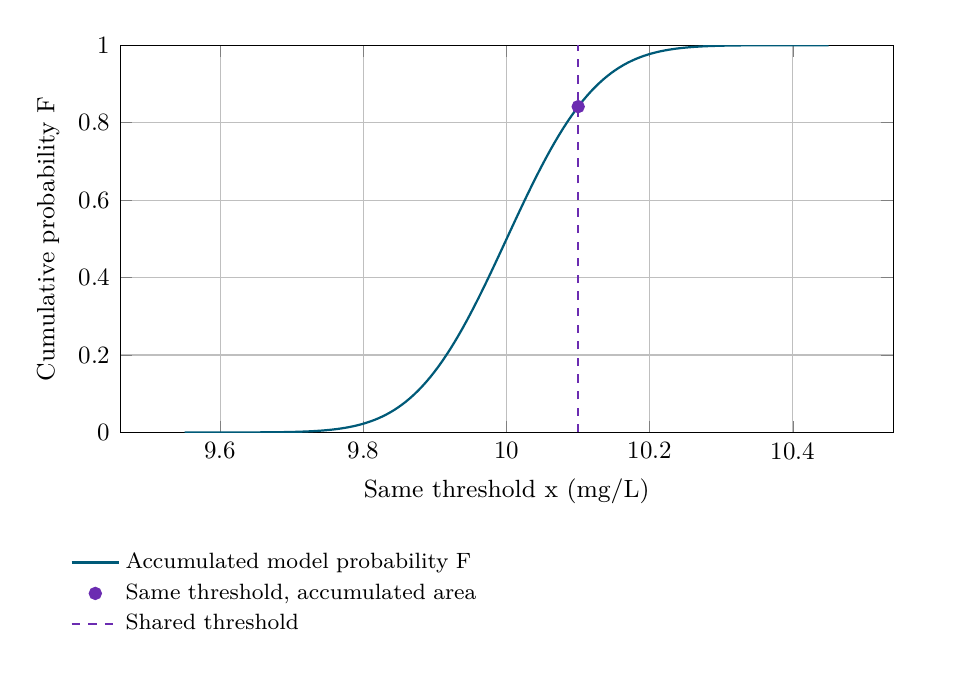
\begin{tikzpicture}
\begin{axis}[width=0.94\linewidth,
height=6.5cm,
scale only axis=false,
grid=major,
tick label style={font=\small},
label style={font=\small},
xlabel={Same threshold x (mg/L)},
ylabel={Cumulative probability F},
legend style={font=\footnotesize,draw=none,at={(0.5,-0.28)},anchor=north,legend columns=1,text width=0.85\linewidth,align=left},
unbounded coords=jump,
scaled ticks=false,
ymin=0,
ymax=1]
\addplot[color=pcd1,thick,mark=none] coordinates {(9.55,0.000003397673124730176) (9.555625000000001,0.000004420216158374301) (9.561250000000001,0.0000057330496867211774) (9.566875000000001,0.000007413261180173364) (9.572500000000002,0.000009556864737291614) (9.578125,0.000012283023933861438) (9.58375,0.000015739107093534205) (9.589375,0.000020106712358389264) (9.595,0.0000256088164740422) (9.600625,0.000032518218358217713) (9.606250000000001,0.00004116746597160116) (9.611875000000001,0.000051960472337781745) (9.6175,0.00006538604324270632) (9.623125,0.00008203355454697703) (9.62875,0.00010261103040967494) (9.634375,0.00012796588416993468) (9.64,0.00015910859015753738) (9.645625,0.00019723955618442874) (9.651250000000001,0.00024377946167532) (9.656875000000001,0.00030040331400853736) (9.662500000000001,0.00036907845427508576) (9.668125,0.00045210671191135454) (9.67375,0.0005521708641184592) (9.679375,0.0006723854993109401) (9.685,0.000816352312828576) (9.690625,0.0009882197767736814) (9.696250000000001,0.0011927470233527508) (9.701875000000001,0.0014353716620997075) (9.7075,0.0017222811158676022) (9.713125,0.0020604869090423677) (9.71875,0.002457901175196685) (9.724375,0.0029234144721869497) (9.73,0.003466973803040703) (9.735625,0.004099659544228397) (9.74125,0.004833759783190674) (9.746875000000001,0.005682840369249544) (9.752500000000001,0.006661808791982947) (9.758125,0.007786969825219256) (9.76375,0.009076070720048795) (9.769375,0.010548333604143605) (9.775,0.012224472655044796) (9.780625,0.014126693569726718) (9.78625,0.016278672859386754) (9.791875000000001,0.018705514564202216) (9.7975,0.02143368211415262) (9.803125,0.024490903264233047) (9.80875,0.02790604630930692) (9.814375,0.03170896613765623) (9.82,0.03593031911292592) (9.825625,0.040601346279518474) (9.83125,0.04575362496174157) (9.836875000000001,0.05141878946481937) (9.842500000000001,0.05762822227615416) (9.848125,0.06441271789526815) (9.85375,0.07180212217541582) (9.859375,0.07982495082140495) (9.865,0.08850799143740218) (9.870625,0.09787589423432819) (9.87625,0.10795075716732572) (9.881875,0.11875171185746636) (9.8875,0.13029451713680718) (9.893125,0.14259116742165434) (9.89875,0.15564952334676752) (9.904375,0.16947297216771934) (9.91,0.1840601253467598) (9.915625,0.19940456047137362) (9.92125,0.21549461421005578) (9.926875,0.23231323238790907) (9.932500000000001,0.24983788247178002) (9.938125,0.2680405328024058) (9.94375,0.2868877018163639) (9.949375,0.306340579285026) (9.955,0.32635522028792013) (9.960625,0.3468828112631477) (9.96625,0.3678700060714789) (9.971875,0.38925932860793994) (9.9775,0.41098963713126696) (9.983125,0.4329966441933256) (9.98875,0.4552134848717433) (9.994375,0.47757132497222066) (10,0.5) (10.005625,0.5224286750277793) (10.01125,0.5447865151282567) (10.016875,0.5670033558066744) (10.0225,0.5890103628687331) (10.028125,0.61074067139206) (10.03375,0.6321299939285211) (10.039375,0.6531171887368523) (10.045,0.6736447797120799) (10.050625,0.693659420714974) (10.05625,0.7131122981836361) (10.061875,0.7319594671975942) (10.067499999999999,0.75016211752822) (10.073125,0.7676867676120909) (10.07875,0.7845053857899442) (10.084375,0.8005954395286263) (10.09,0.8159398746532402) (10.095625,0.8305270278322807) (10.10125,0.8443504766532325) (10.106875,0.8574088325783457) (10.1125,0.8697054828631928) (10.118125,0.8812482881425336) (10.12375,0.8920492428326743) (10.129375,0.9021241057656718) (10.135,0.9114920085625978) (10.140625,0.920175049178595) (10.14625,0.9281978778245842) (10.151875,0.9355872821047319) (10.157499999999999,0.9423717777238458) (10.163124999999999,0.9485812105351806) (10.16875,0.9542463750382584) (10.174375,0.9593986537204815) (10.18,0.9640696808870741) (10.185625,0.9682910338623437) (10.19125,0.9720939536906931) (10.196875,0.9755090967357669) (10.2025,0.9785663178858474) (10.208124999999999,0.9812944854357978) (10.21375,0.9837213271406132) (10.219375,0.9858733064302733) (10.225,0.9877755273449552) (10.230625,0.9894516663958564) (10.23625,0.9909239292799512) (10.241875,0.9922130301747808) (10.247499999999999,0.993338191208017) (10.253124999999999,0.9943171596307504) (10.25875,0.9951662402168093) (10.264375,0.9959003404557716) (10.27,0.9965330261969593) (10.275625,0.9970765855278131) (10.28125,0.9975420988248033) (10.286875,0.9979395130909576) (10.2925,0.9982777188841324) (10.298124999999999,0.9985646283379003) (10.303749999999999,0.9988072529766473) (10.309375,0.9990117802232263) (10.315,0.9991836476871714) (10.320625,0.9993276145006891) (10.32625,0.9994478291358816) (10.331875,0.9995478932880887) (10.337499999999999,0.9996309215457249) (10.343124999999999,0.9996995966859915) (10.348749999999999,0.9997562205383247) (10.354375,0.9998027604438156) (10.36,0.9998408914098424) (10.365625,0.99987203411583) (10.37125,0.9998973889695904) (10.376875,0.999917966445453) (10.3825,0.9999346139567573) (10.388124999999999,0.9999480395276622) (10.393749999999999,0.9999588325340284) (10.399375,0.9999674817816417) (10.405,0.9999743911835259) (10.410625,0.9999798932876416) (10.41625,0.9999842608929065) (10.421875,0.9999877169760661) (10.427499999999998,0.9999904431352628) (10.433124999999999,0.9999925867388199) (10.438749999999999,0.9999942669503132) (10.444374999999999,0.9999955797838416) (10.45,0.9999966023268753)};
\addlegendentry{Accumulated model probability F}
\addplot[color=pcd2,thick,only marks,mark=*] coordinates {(10.1,0.8413447460685424)};
\addlegendentry{Same threshold, accumulated area}
\addplot[color=pcd2,dashed,thick] coordinates {(10.1,0) (10.1,1)};
\addlegendentry{Shared threshold}
\end{axis}
\end{tikzpicture}
\end{center}

% Full-precision experiment details: {"blockId":"ex:pc-n10-v--block","parameters":[{"key":"location","label":"Assumed model expectation (mg/L)","value":10},{"key":"scale","label":"Assumed model SD (mg/L)","value":0.1},{"key":"threshold","label":"Shared concentration threshold (mg/L)","value":10.1},{"key":"width","label":"Unused interval half-width in cumulative view (mg/L)","value":0.1},{"key":"probability","label":"Chosen cumulative probability p","value":0.95},{"key":"family","label":"Model: 0 smooth bell, 1 bounded flat","value":0},{"key":"M","label":"Fixed reference replay count","value":1000},{"key":"seed","label":"Fixed reference replay seed","value":20261102},{"key":"view","label":"Question: 1 probability from threshold, 2 threshold from p","value":1}],"readouts":[{"label":"Shared threshold (mg/L)","value":10.1},{"label":"Accumulated probability F(x)","value":0.8413447460685424},{"label":"Model density f(x)","value":2.419707245191442},{"label":"Chosen cumulative probability p","value":0.95},{"label":"Inverse-CDF threshold (mg/L)","value":10.164485362695148}],"note":"PDF area equals the CDF ordinate. The density gives the local rate at which cumulative probability increases.","markers":[[{"x":10.1,"label":"Shared threshold"}],[{"x":10.1,"label":"Shared threshold"}]]}

\medskip

\par\medskip
\noindent\begin{minipage}{\linewidth}
\refstepcounter{equation}\label{material-d5d05efcdd8a06801dd5a158b8891a5dc14f41a3402fa3fbb5c37dc23548257b}
\noindent\textbf{Eq.~\ref*{material-d5d05efcdd8a06801dd5a158b8891a5dc14f41a3402fa3fbb5c37dc23548257b}.} A concentration threshold obtained from a prescribed upper-tail probability.\par\nopagebreak
\begin{center}\begin{adjustbox}{max width=\linewidth}$\displaystyle \begin{gathered}z^*=\Phi^{-1}(0.99)\approx2.32635\\x^*=\mu+z^*\sigma\\\approx10.23263\;\mathrm{mg/L}\end{gathered}$\end{adjustbox}\end{center}

\par\noindent\textbf{Symbols}

\begin{itemize}\setlength{\itemsep}{1pt}\setlength{\parsep}{0pt}
\item \textbf{\ensuremath{\Phi}, \ensuremath{\Phi}\ensuremath{{}^-}\ensuremath{{}^1}}: Standard-normal CDF and its inverse quantile function.
\item \textbf{z}*: Chosen standardized threshold (dimensionless), here the 0.99 quantile.
\item \textbf{x}*: Corresponding concentration threshold (mg/L).
\item \textbf{\ensuremath{\mu}}: Known expectation, 10.00 mg/L.
\item \textbf{\ensuremath{\sigma}}: Known SD, 0.10 mg/L.
\item \textbf{*}: Superscript star identifying a chosen threshold.
\item \textbf{+, =, \ensuremath{\approx}}: Addition, equality and approximate equality; adjacent factors multiply.
\end{itemize}

Superscript \ensuremath{-}1 denotes the inverse function. Under the model, 1\% of individual results exceed the unrounded threshold; the displayed 10.233 mg/L is rounded.

\end{minipage}\par
\medskip

\par\medskip
\Needspace{8\baselineskip}
\refstepcounter{listing}\label{material-9c0e8d6352f7ca3835e957a15da673db61154f61b7ffec37dda6c8bd12221b02}
\noindent\textbf{Listing~\ref*{material-9c0e8d6352f7ca3835e957a15da673db61154f61b7ffec37dda6c8bd12221b02}.} R comparison of empirical sample fractions and fixed model probabilities.\par\nopagebreak
\begin{Verbatim}[fontsize=\footnotesize,breaklines=true,breakanywhere=true]
# Same deterministic 1000-draw sample as the saved histogram.
M <- 1000; mu <- 10.00; sigma <- 0.10; state <- 20261102
x <- numeric(M)
for(i in seq_len(M)) {
  state <- (16807*state) %% 2147483647
  x[i] <- mu+sigma*qnorm(state/2147483647)
}
Fn <- ecdf(x)
cat('Observed fractions at 9.80, 10.00, 10.20:',Fn(c(9.8,10,10.2)),'\n')
cat('Theoretical CDF at 10.20:',pnorm(10.2,mu,sigma),'\n')
cat('Observed upper fraction:',mean(x>10.2),'\n')
plot(Fn,verticals=FALSE,do.points=FALSE,col='#176b90',lwd=2,
     main='1000 observations versus an assumed model',
     xlab='Nitrate threshold (mg/L)',ylab='Cumulative probability')
curve(pnorm(x,mean=mu,sd=sigma),add=TRUE,col='#a63d21',lwd=2)
legend('topleft',c('Empirical step CDF','Fixed theoretical CDF'),
       col=c('#176b90','#a63d21'),lty=1,bty='n')

\end{Verbatim}

\medskip

\clearpage
\section{The Normal model: location, spread and standardized distance}
The Normal family is a model for variation that can arise when many small additive influences combine under suitable central-limit conditions. Its symmetric density is characterized by a location and a spread. The standard-Normal shape is shown in \hyperref[material-23e8b5c9c2c01857d30a68806961d7261901206f42036ec3b3824a08d7c83ff4]{Fig.~\ref*{material-23e8b5c9c2c01857d30a68806961d7261901206f42036ec3b3824a08d7c83ff4}}. The measurement process and its sampling conditions provide the context for assessing this model.


\par\medskip
\Needspace{10cm}
\refstepcounter{figure}\label{material-23e8b5c9c2c01857d30a68806961d7261901206f42036ec3b3824a08d7c83ff4}
\noindent\textbf{Fig.~\ref*{material-23e8b5c9c2c01857d30a68806961d7261901206f42036ec3b3824a08d7c83ff4}.} The standard-Normal density is symmetric about zero, where it reaches its maximum. The horizontal coordinate is standardized distance and the vertical coordinate is density per standardized unit.\par\nopagebreak
\begin{center}
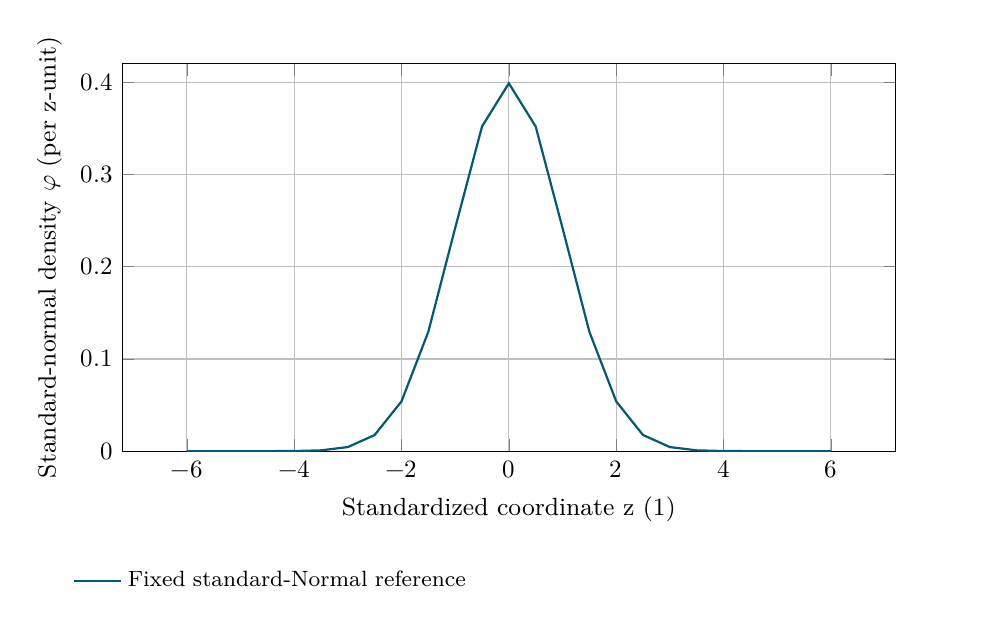
\begin{tikzpicture}
\begin{axis}[width=0.94\linewidth,
height=6.5cm,
scale only axis=false,
grid=major,
tick label style={font=\small},
label style={font=\small},
xlabel={Standardized coordinate z (1)},
ylabel={Standard-normal density \ensuremath{\varphi} (per z-unit)},
legend style={font=\footnotesize,draw=none,at={(0.5,-0.28)},anchor=north,legend columns=1,text width=0.85\linewidth,align=left},
unbounded coords=jump,
scaled ticks=false,
ymin=0,
ymax=0.42]
\addplot[color=pcd1,thick,mark=none] coordinates {(-6,6.076e-9) (-5.5,1.07698e-7) (-5,0.00000148672) (-4.5,0.000015983741) (-4,0.000133830226) (-3.5,0.000872682695) (-3,0.004431848412) (-2.5,0.017528300494) (-2,0.053990966513) (-1.5,0.129517595666) (-1,0.241970724519) (-0.5,0.352065326764) (0,0.398942280401) (0.5,0.352065326764) (1,0.241970724519) (1.5,0.129517595666) (2,0.053990966513) (2.5,0.017528300494) (3,0.004431848412) (3.5,0.000872682695) (4,0.000133830226) (4.5,0.000015983741) (5,0.00000148672) (5.5,1.07698e-7) (6,6.076e-9)};
\addlegendentry{Fixed standard-Normal reference}

\end{axis}
\end{tikzpicture}
\end{center}

\medskip

Within this family, location sets the centre and the standard deviation sets the concentration scale. Subtracting the model mean and dividing by the model standard deviation expresses a result as a dimensionless standardized distance. This transformation allows probabilities from different concentration scales to be read using the same standard-Normal distribution. A concentration difference only acquires a probability meaning after its model spread has been specified.


The standard-Normal density is denoted by \(\varphi\), and its cumulative probability by \(\Phi\). Integrating \(\varphi\) produces \(\Phi\); the displayed error-function identity expresses the same accumulation. In the fixed example, 10.20 mg/L is two standard deviations above the mean, giving cumulative probability about 0.97725 and an upper tail about 0.02275.


Changing spread while retaining the same centre changes the probability beyond a fixed concentration limit (\hyperref[material-954c0058b9380916a12ffdf3a9d33d8db9642a5bea9fb1ad653adc889dd6c4c6]{Fig.~\ref*{material-954c0058b9380916a12ffdf3a9d33d8db9642a5bea9fb1ad653adc889dd6c4c6}}). For a limit above the mean, a broader Normal model places more probability in the upper tail. The familiar coverage of standard-deviation bands follows from the Normal model; \hyperref[material-e6abe340f68564bc23136c31cd1f7301d0d0f695ec7173a348896025afaeef69]{Fig.~\ref*{material-e6abe340f68564bc23136c31cd1f7301d0d0f695ec7173a348896025afaeef69}} contrasts a central band with a one-sided limit. Interpreting such a band as an analytical decision limit additionally requires a stated decision rule and its assumptions.


\par\medskip
\Needspace{10cm}
\refstepcounter{figure}\label{material-954c0058b9380916a12ffdf3a9d33d8db9642a5bea9fb1ad653adc889dd6c4c6}
\noindent\textbf{Fig.~\ref*{material-954c0058b9380916a12ffdf3a9d33d8db9642a5bea9fb1ad653adc889dd6c4c6}.} Two Normal models share expectation 10.00 mg/L and the marked result 10.20 mg/L. Known SDs of 0.10 and 0.20 mg/L put that result two SD above the expectation for A and one SD above it for B.\par\nopagebreak
\begin{center}
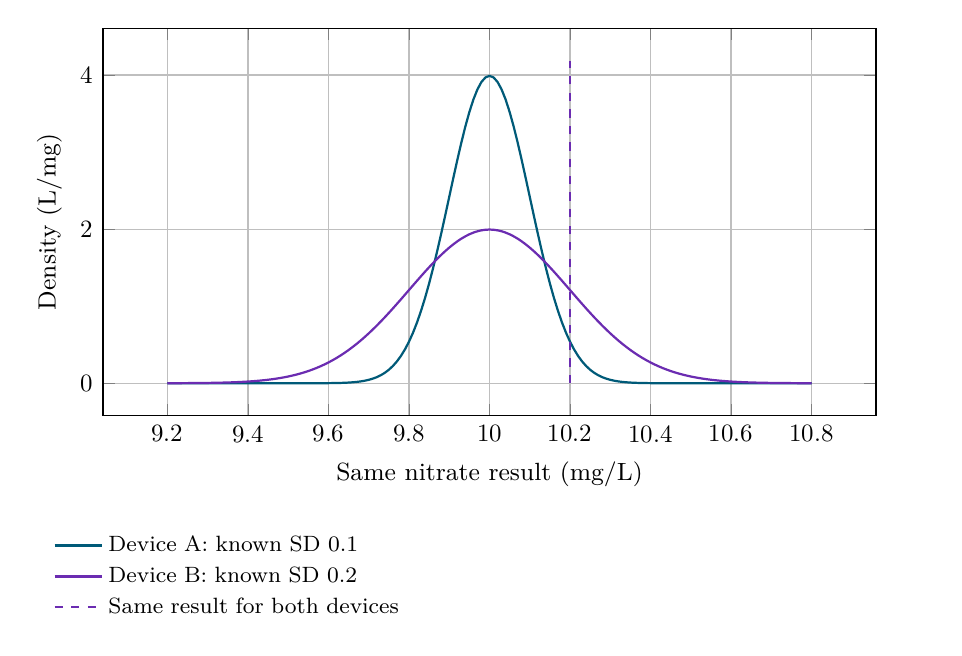
\begin{tikzpicture}
\begin{axis}[width=0.94\linewidth,
height=6.5cm,
scale only axis=false,
grid=major,
tick label style={font=\small},
label style={font=\small},
xlabel={Same nitrate result (mg/L)},
ylabel={Density (L/mg)},
legend style={font=\footnotesize,draw=none,at={(0.5,-0.28)},anchor=north,legend columns=1,text width=0.85\linewidth,align=left},
unbounded coords=jump,
scaled ticks=false]
\addplot[color=pcd1,thick,mark=none] coordinates {(9.2,5.0522710835366054e-14) (9.209999999999999,1.1187956214351021e-13) (9.219999999999999,2.452855285696215e-13) (9.229999999999999,5.324148372252415e-13) (9.239999999999998,1.1441564901799988e-12) (9.25,2.43432053302901e-12) (9.26,5.127753636796591e-12) (9.27,1.0693837871541298e-11) (9.28,2.207989963137045e-11) (9.29,4.513543677205229e-11) (9.299999999999999,9.134720408363913e-11) (9.309999999999999,1.8303322170154155e-10) (9.32,3.630961501791865e-10) (9.33,7.131328123996102e-10) (9.34,1.3866799941653025e-9) (9.35,2.6695566147627856e-9) (9.36,5.088140281644876e-9) (9.37,9.601433370311856e-9) (9.379999999999999,1.7937839079639712e-8) (9.389999999999999,3.3178842435470456e-8) (9.399999999999999,6.075882849822767e-8) (9.41,1.1015763624682425e-7) (9.42,1.97731964062446e-7) (9.43,3.5139550948203835e-7) (9.44,6.182620500165671e-7) (9.45,0.0000010769760042542857) (9.459999999999999,0.0000018573618445552007) (9.469999999999999,0.000003171349216715784) (9.48,0.000005361035344697737) (9.49,0.000008972435162383432) (9.5,0.000014867195147342979) (9.51,0.00002438960745893335) (9.52,0.00003961299091031991) (9.53,0.00006369825178866908) (9.54,0.00010140852065486346) (9.549999999999999,0.00015983741106904707) (9.559999999999999,0.0002494247129005216) (9.57,0.00038535196742087543) (9.58,0.0005894306775654005) (9.59,0.000892616571771323) (9.6,0.0013383022576488345) (9.61,0.0019865547139276828) (9.62,0.002919469257914515) (9.629999999999999,0.004247802705507359) (9.64,0.00611901930113785) (9.65,0.008726826950457709) (9.66,0.012322191684730253) (9.67,0.017225689390536765) (9.68,0.02384088201464821) (9.69,0.03266819056199869) (9.7,0.04431848411937913) (9.709999999999999,0.059525324197756954) (9.719999999999999,0.07915451582979711) (9.73,0.10420934814422717) (9.74,0.1358296923368569) (9.75,0.17528300493568538) (9.76,0.2239453029484278) (9.77,0.283270377416009) (9.78,0.35474592846230935) (9.79,0.4398359598042641) (9.8,0.5399096651318882) (9.81,0.6561581477467721) (9.82,0.7895015830089458) (9.83,0.9404907737688704) (9.84,1.109208346794553) (9.85,1.2951759566589105) (9.86,1.4972746563574368) (9.87,1.7136859204780563) (9.879999999999999,1.9418605498321064) (9.89,2.178521770325519) (9.9,2.419707245191442) (9.91,2.660852498987552) (9.92,2.896915527614826) (9.93,3.1225393336676066) (9.94,3.3322460289179867) (9.95,3.5206532676429823) (9.96,3.682701403033246) (9.97,3.8138781546052485) (9.98,3.9104269397545623) (9.99,3.969525474770119) (10,3.989422804014327) (10.01,3.969525474770119) (10.02,3.9104269397545623) (10.03,3.8138781546052485) (10.04,3.682701403033246) (10.05,3.5206532676429823) (10.06,3.3322460289179867) (10.07,3.1225393336676066) (10.08,2.896915527614826) (10.09,2.660852498987552) (10.1,2.419707245191442) (10.11,2.178521770325519) (10.120000000000001,1.9418605498321064) (10.13,1.7136859204780563) (10.14,1.4972746563574368) (10.15,1.2951759566589105) (10.16,1.109208346794553) (10.17,0.9404907737688704) (10.18,0.7895015830089458) (10.19,0.6561581477467721) (10.2,0.5399096651318882) (10.21,0.4398359598042641) (10.22,0.35474592846230935) (10.23,0.283270377416009) (10.24,0.2239453029484278) (10.25,0.17528300493568538) (10.26,0.1358296923368569) (10.27,0.10420934814422717) (10.280000000000001,0.07915451582979711) (10.290000000000001,0.059525324197756954) (10.3,0.04431848411937913) (10.31,0.03266819056199869) (10.32,0.02384088201464821) (10.33,0.017225689390536765) (10.34,0.012322191684730253) (10.35,0.008726826950457709) (10.36,0.00611901930113785) (10.370000000000001,0.004247802705507359) (10.38,0.002919469257914515) (10.39,0.0019865547139276828) (10.4,0.0013383022576488345) (10.41,0.000892616571771323) (10.42,0.0005894306775654005) (10.43,0.00038535196742087543) (10.440000000000001,0.0002494247129005216) (10.450000000000001,0.00015983741106904707) (10.46,0.00010140852065486346) (10.47,0.00006369825178866908) (10.48,0.00003961299091031991) (10.49,0.00002438960745893335) (10.5,0.000014867195147342979) (10.51,0.000008972435162383432) (10.52,0.000005361035344697737) (10.530000000000001,0.000003171349216715784) (10.540000000000001,0.0000018573618445552007) (10.55,0.0000010769760042542857) (10.56,6.182620500165671e-7) (10.57,3.5139550948203835e-7) (10.58,1.97731964062446e-7) (10.59,1.1015763624682425e-7) (10.600000000000001,6.075882849822767e-8) (10.610000000000001,3.3178842435470456e-8) (10.620000000000001,1.7937839079639712e-8) (10.63,9.601433370311856e-9) (10.64,5.088140281644876e-9) (10.65,2.6695566147627856e-9) (10.66,1.3866799941653025e-9) (10.67,7.131328123996102e-10) (10.68,3.630961501791865e-10) (10.690000000000001,1.8303322170154155e-10) (10.700000000000001,9.134720408363913e-11) (10.71,4.513543677205229e-11) (10.72,2.207989963137045e-11) (10.73,1.0693837871541298e-11) (10.74,5.127753636796591e-12) (10.75,2.43432053302901e-12) (10.760000000000002,1.1441564901799988e-12) (10.770000000000001,5.324148372252415e-13) (10.780000000000001,2.452855285696215e-13) (10.790000000000001,1.1187956214351021e-13) (10.8,5.0522710835366054e-14)};
\addlegendentry{Device A: known SD 0.1}
\addplot[color=pcd2,thick,mark=none] coordinates {(9.2,0.0006691511288244173) (9.209999999999999,0.0008162820438311955) (9.219999999999999,0.0009932773569638414) (9.229999999999999,0.0012056329011299364) (9.239999999999998,0.0014597346289572574) (9.25,0.0017629784118372272) (9.26,0.00212390135275375) (9.27,0.002552324871720907) (9.28,0.003059509650568827) (9.29,0.003658322314151496) (9.299999999999999,0.004363413475228719) (9.309999999999999,0.005191406478306941) (9.32,0.0061610958423651266) (9.33,0.007293654023333737) (9.34,0.008612844695268383) (9.35,0.010145240286498774) (9.36,0.011920441007324105) (9.37,0.013971292074397061) (9.379999999999999,0.016334095280999345) (9.389999999999999,0.019048810491108677) (9.399999999999999,0.022159242059689565) (9.41,0.025713204615269766) (9.42,0.02976266209887924) (9.43,0.03436383345306974) (9.44,0.039577257914899536) (9.45,0.04546781250795482) (9.459999999999999,0.05210467407211232) (9.469999999999999,0.05956121803802499) (9.48,0.06791484616842845) (9.49,0.07724673567197607) (9.5,0.08764150246784269) (9.51,0.09918677195897639) (9.52,0.1119726514742139) (9.53,0.126091099575971) (9.54,0.1416351887080045) (9.549999999999999,0.15869825917833516) (9.559999999999999,0.17737296423115467) (9.57,0.19775020794685164) (9.58,0.21991797990213616) (9.59,0.2439600928959134) (9.6,0.2699548325659393) (9.61,0.29797353034407875) (9.62,0.3280790738733805) (9.629999999999999,0.36032437168108666) (9.64,0.3947507915044729) (9.65,0.431386594132559) (9.66,0.4702453868844352) (9.67,0.5113246228198898) (9.68,0.5546041733972765) (9.69,0.6000450034849256) (9.7,0.6475879783294552) (9.709999999999999,0.6971528322267968) (9.719999999999999,0.7486373281787184) (9.73,0.8019166367096003) (9.74,0.8568429602390379) (9.75,0.9132454269451096) (9.76,0.9709302749160634) (9.77,1.0296813435998713) (9.78,1.089260885162749) (9.79,1.1494107034211603) (9.8,1.209853622595721) (9.81,1.2702952823459481) (9.82,1.330426249493776) (9.83,1.389924430654983) (9.84,1.448457763807413) (9.85,1.50568716077402) (9.86,1.5612696668338033) (9.87,1.6148617983395674) (9.879999999999999,1.6661230144589934) (9.89,1.7147192750969222) (9.9,1.7603266338214991) (9.91,1.8026348123082405) (9.92,1.8413507015166164) (9.93,1.8762017345846886) (9.94,1.9069390773026191) (9.95,1.9333405840142444) (9.96,1.9552134698772812) (9.97,1.9723966545394456) (9.98,1.9847627373850596) (9.99,1.9922195704738201) (10,1.9947114020071635) (10.01,1.9922195704738201) (10.02,1.9847627373850596) (10.03,1.9723966545394456) (10.04,1.9552134698772812) (10.05,1.9333405840142444) (10.06,1.9069390773026191) (10.07,1.8762017345846886) (10.08,1.8413507015166164) (10.09,1.8026348123082405) (10.1,1.7603266338214991) (10.11,1.7147192750969222) (10.120000000000001,1.6661230144589934) (10.13,1.6148617983395674) (10.14,1.5612696668338033) (10.15,1.50568716077402) (10.16,1.448457763807413) (10.17,1.389924430654983) (10.18,1.330426249493776) (10.19,1.2702952823459481) (10.2,1.209853622595721) (10.21,1.1494107034211603) (10.22,1.089260885162749) (10.23,1.0296813435998713) (10.24,0.9709302749160634) (10.25,0.9132454269451096) (10.26,0.8568429602390379) (10.27,0.8019166367096003) (10.280000000000001,0.7486373281787184) (10.290000000000001,0.6971528322267968) (10.3,0.6475879783294552) (10.31,0.6000450034849256) (10.32,0.5546041733972765) (10.33,0.5113246228198898) (10.34,0.4702453868844352) (10.35,0.431386594132559) (10.36,0.3947507915044729) (10.370000000000001,0.36032437168108666) (10.38,0.3280790738733805) (10.39,0.29797353034407875) (10.4,0.2699548325659393) (10.41,0.2439600928959134) (10.42,0.21991797990213616) (10.43,0.19775020794685164) (10.440000000000001,0.17737296423115467) (10.450000000000001,0.15869825917833516) (10.46,0.1416351887080045) (10.47,0.126091099575971) (10.48,0.1119726514742139) (10.49,0.09918677195897639) (10.5,0.08764150246784269) (10.51,0.07724673567197607) (10.52,0.06791484616842845) (10.530000000000001,0.05956121803802499) (10.540000000000001,0.05210467407211232) (10.55,0.04546781250795482) (10.56,0.039577257914899536) (10.57,0.03436383345306974) (10.58,0.02976266209887924) (10.59,0.025713204615269766) (10.600000000000001,0.022159242059689565) (10.610000000000001,0.019048810491108677) (10.620000000000001,0.016334095280999345) (10.63,0.013971292074397061) (10.64,0.011920441007324105) (10.65,0.010145240286498774) (10.66,0.008612844695268383) (10.67,0.007293654023333737) (10.68,0.0061610958423651266) (10.690000000000001,0.005191406478306941) (10.700000000000001,0.004363413475228719) (10.71,0.003658322314151496) (10.72,0.003059509650568827) (10.73,0.002552324871720907) (10.74,0.00212390135275375) (10.75,0.0017629784118372272) (10.760000000000002,0.0014597346289572574) (10.770000000000001,0.0012056329011299364) (10.780000000000001,0.0009932773569638414) (10.790000000000001,0.0008162820438311955) (10.8,0.0006691511288244173)};
\addlegendentry{Device B: known SD 0.2}
\addplot[color=pcd2,dashed,thick] coordinates {(10.2,0) (10.2,4.188893944215043)};
\addlegendentry{Same result for both devices}
\end{axis}
\end{tikzpicture}
\end{center}

% Full-precision experiment details: {"blockId":"ex:p1-n13-v--block","parameters":[{"key":"sigma","label":"True method SD (mg/L), assumed","value":0.1},{"key":"mu","label":"Assumed method expectation (mg/L)","value":10},{"key":"threshold","label":"Chosen threshold (mg/L)","value":10.2},{"key":"alpha","label":"Chosen upper-tail rate","value":0.01},{"key":"inverse","label":"Inverse mode: 0 threshold, 1 rate","value":0},{"key":"comparisonSigma","label":"Device B known model SD (mg/L)","value":0.2},{"key":"view","label":"Authored two-model comparison view","value":4}],"readouts":[{"label":"Threshold","value":10.2},{"label":"Standardized distance","value":1.999999999999993},{"label":"Device B standardized distance","value":0.9999999999999964}],"note":"Probabilities are areas under the density over the full model domain. The displayed examples use explicitly specified model parameters. Both known-parameter models use the same observed concentration and their specified population standard deviations.","markers":[[{"x":10.2,"label":"Same result for both devices"}]]}

\medskip

\par\medskip
\Needspace{10cm}
\refstepcounter{figure}\label{material-e6abe340f68564bc23136c31cd1f7301d0d0f695ec7173a348896025afaeef69}
\noindent\textbf{Fig.~\ref*{material-e6abe340f68564bc23136c31cd1f7301d0d0f695ec7173a348896025afaeef69}.} The panels compare a one-sided upper 1\% limit, about 10.233 mg/L, with a central two-SD band under the Normal model with expectation 10.00 mg/L and SD 0.10 mg/L. The central band contains about 95.45\% of the probability, leaving about 4.550\% across both tails.\par\nopagebreak
\begin{center}
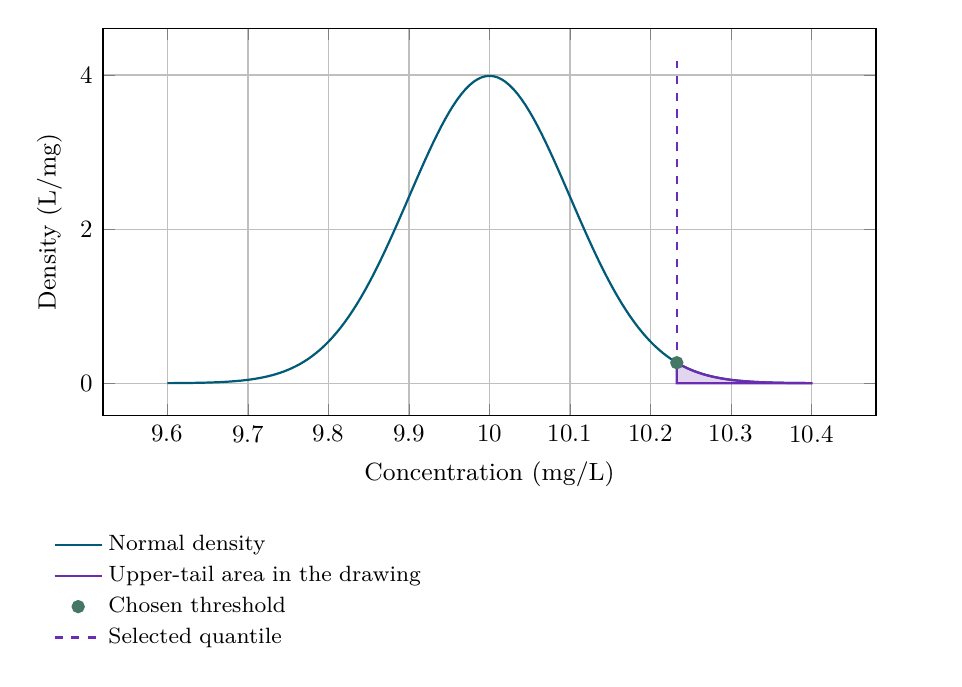
\begin{tikzpicture}
\begin{axis}[width=0.94\linewidth,
height=6.5cm,
scale only axis=false,
grid=major,
tick label style={font=\small},
label style={font=\small},
xlabel={Concentration (mg/L)},
ylabel={Density (L/mg)},
legend style={font=\footnotesize,draw=none,at={(0.5,-0.28)},anchor=north,legend columns=1,text width=0.85\linewidth,align=left},
unbounded coords=jump,
scaled ticks=false]
\addplot[color=pcd1,thick,mark=none] coordinates {(9.6,0.0013383022576488345) (9.605,0.0016325640876624478) (9.61,0.0019865547139276828) (9.615,0.002411265802259954) (9.62,0.002919469257914515) (9.625,0.0035259568236744544) (9.629999999999999,0.004247802705507359) (9.635,0.005104649743441814) (9.64,0.00611901930113785) (9.645,0.007316644628302992) (9.65,0.008726826950457709) (9.655,0.010382812956613882) (9.66,0.012322191684730253) (9.665,0.014587308046667044) (9.67,0.017225689390536765) (9.674999999999999,0.020290480572996972) (9.68,0.02384088201464821) (9.685,0.027942584148794893) (9.69,0.03266819056199869) (9.695,0.03809762098221841) (9.7,0.04431848411937913) (9.705,0.05142640923053953) (9.709999999999999,0.059525324197756954) (9.715,0.06872766690613948) (9.719999999999999,0.07915451582979711) (9.725,0.09093562501590964) (9.73,0.10420934814422717) (9.735,0.11912243607604998) (9.74,0.1358296923368569) (9.745,0.15449347134394867) (9.75,0.17528300493568538) (9.754999999999999,0.19837354391794843) (9.76,0.2239453029484278) (9.765,0.25218219915194723) (9.77,0.283270377416009) (9.775,0.31739651835667665) (9.78,0.35474592846230935) (9.785,0.39550041589370327) (9.79,0.4398359598042641) (9.795,0.4879201857918268) (9.8,0.5399096651318882) (9.805,0.5959470606881575) (9.81,0.6561581477467721) (9.815,0.7206487433621733) (9.82,0.7895015830089458) (9.825,0.8627731882651044) (9.83,0.9404907737688704) (9.834999999999999,1.0226492456397647) (9.84,1.109208346794553) (9.845,1.2000900069698677) (9.85,1.2951759566589105) (9.855,1.3943056644536114) (9.86,1.4972746563574368) (9.865,1.6038332734192007) (9.87,1.7136859204780563) (9.875,1.8264908538902191) (9.879999999999999,1.9418605498321064) (9.885,2.0593626871997426) (9.89,2.178521770325519) (9.895,2.2988214068423205) (9.9,2.419707245191442) (9.905,2.5405905646918745) (9.91,2.660852498987552) (9.915,2.7798488613099446) (9.92,2.896915527614826) (9.925,3.01137432154806) (9.93,3.1225393336676066) (9.935,3.2297235966791535) (9.94,3.3322460289179867) (9.945,3.4294385501938445) (9.95,3.5206532676429823) (9.955,3.605269624616481) (9.96,3.682701403033246) (9.965,3.7524034691693773) (9.97,3.8138781546052485) (9.975,3.8666811680284887) (9.98,3.9104269397545623) (9.985,3.944793309078886) (9.99,3.969525474770119) (9.995,3.9844391409476385) (10,3.989422804014327) (10.005,3.9844391409476385) (10.01,3.969525474770119) (10.015,3.944793309078886) (10.02,3.9104269397545623) (10.025,3.8666811680284887) (10.03,3.8138781546052485) (10.035,3.7524034691693773) (10.04,3.682701403033246) (10.045,3.605269624616481) (10.05,3.5206532676429823) (10.055,3.4294385501938445) (10.06,3.3322460289179867) (10.065,3.2297235966791535) (10.07,3.1225393336676066) (10.075,3.01137432154806) (10.08,2.896915527614826) (10.085,2.7798488613099446) (10.09,2.660852498987552) (10.095,2.5405905646918745) (10.1,2.419707245191442) (10.105,2.2988214068423205) (10.11,2.178521770325519) (10.115,2.0593626871997426) (10.120000000000001,1.9418605498321064) (10.125,1.8264908538902191) (10.13,1.7136859204780563) (10.135,1.6038332734192007) (10.14,1.4972746563574368) (10.145,1.3943056644536114) (10.15,1.2951759566589105) (10.155,1.2000900069698677) (10.16,1.109208346794553) (10.165000000000001,1.0226492456397647) (10.17,0.9404907737688704) (10.175,0.8627731882651044) (10.18,0.7895015830089458) (10.185,0.7206487433621733) (10.19,0.6561581477467721) (10.195,0.5959470606881575) (10.2,0.5399096651318882) (10.205,0.4879201857918268) (10.21,0.4398359598042641) (10.215,0.39550041589370327) (10.22,0.35474592846230935) (10.225,0.31739651835667665) (10.23,0.283270377416009) (10.235,0.25218219915194723) (10.24,0.2239453029484278) (10.245000000000001,0.19837354391794843) (10.25,0.17528300493568538) (10.255,0.15449347134394867) (10.26,0.1358296923368569) (10.265,0.11912243607604998) (10.27,0.10420934814422717) (10.275,0.09093562501590964) (10.280000000000001,0.07915451582979711) (10.285,0.06872766690613948) (10.290000000000001,0.059525324197756954) (10.295,0.05142640923053953) (10.3,0.04431848411937913) (10.305,0.03809762098221841) (10.31,0.03266819056199869) (10.315,0.027942584148794893) (10.32,0.02384088201464821) (10.325000000000001,0.020290480572996972) (10.33,0.017225689390536765) (10.335,0.014587308046667044) (10.34,0.012322191684730253) (10.345,0.010382812956613882) (10.35,0.008726826950457709) (10.355,0.007316644628302992) (10.36,0.00611901930113785) (10.365,0.005104649743441814) (10.370000000000001,0.004247802705507359) (10.375,0.0035259568236744544) (10.38,0.002919469257914515) (10.385,0.002411265802259954) (10.39,0.0019865547139276828) (10.395,0.0016325640876624478) (10.4,0.0013383022576488345)};
\addlegendentry{Normal density}
\addplot[color=pcd2,thick,mark=none,fill=pcd2,fill opacity=0.2] coordinates {(10.232634787404084,0.2665214220345802) (10.233680819982808,0.2600998400190464) (10.234726852561533,0.25380520747589713) (10.235772885140257,0.24763581287697248) (10.236818917718981,0.24158994559791636) (10.237864950297707,0.23566589663569545) (10.238910982876432,0.22986195930781392) (10.239957015455156,0.2241764299330676) (10.24100304803388,0.2186076084940467) (10.242049080612604,0.21315379928126016) (10.243095113191329,0.20781331151897592) (10.244141145770053,0.2025844599728164) (10.245187178348777,0.19746556553917222) (10.246233210927503,0.19245495581649585) (10.247279243506227,0.18755096565861454) (10.248325276084952,0.18275193771003012) (10.249371308663676,0.17805622292348422) (10.2504173412424,0.17346218105978065) (10.251463373821124,0.16896818117004336) (10.252509406399849,0.16457260206054206) (10.253555438978573,0.1602738327402331) (10.254601471557297,0.1560702728511744) (10.255647504136023,0.15196033308197257) (10.256693536714748,0.14794243556448122) (10.257739569293472,0.14401501425382687) (10.258785601872196,0.14017651529209507) (10.25983163445092,0.13642539735576878) (10.260877667029645,0.1327601319871673) (10.261923699608369,0.1291792039100897) (10.262969732187093,0.1256811113298822) (10.26401576476582,0.12226436621814672) (10.265061797344543,0.1189274945823557) (10.266107829923268,0.11566903672052119) (10.267153862501992,0.11248754746127375) (10.268199895080716,0.10938159638950862) (10.26924592765944,0.10634976805788257) (10.270291960238165,0.10339066218440761) (10.271337992816889,0.10050289383639827) (10.272384025395615,0.09768509360102605) (10.27343005797434,0.09493590774277247) (10.274476090553064,0.0922539983479731) (10.275522123131788,0.08963804345681572) (10.276568155710512,0.08708673718298965) (10.277614188289236,0.08459878982128566) (10.27866022086796,0.08217292794341366) (10.279706253446685,0.079807894482312) (10.28075228602541,0.07750244880522225) (10.281798318604135,0.07525536677580019) (10.28284435118286,0.07306544080556204) (10.283890383761584,0.07093147989488312) (10.284936416340308,0.06885230966390081) (10.285982448919032,0.06682677237354011) (10.287028481497757,0.06485372693695778) (10.28807451407648,0.0629320489216758) (10.289120546655205,0.0610606305426762) (10.290166579233931,0.05923838064672577) (10.291212611812655,0.057464224688218594) (10.29225864439138,0.055737104696758924) (10.293304676970104,0.05405597923681244) (10.294350709548828,0.05241982335964428) (10.295396742127553,0.05082762854782411) (10.296442774706277,0.049278402652556626) (10.297488807285001,0.04777116982409348) (10.298534839863725,0.046304970435483477) (10.299580872442451,0.04487886099990931) (10.300626905021176,0.04349191408187632) (10.3016729375999,0.0421432182024621) (10.302718970178624,0.04083187773892002) (10.303765002757348,0.039557012818839374) (10.304811035336073,0.03831775920911424) (10.305857067914797,0.037113268199951525) (10.306903100493521,0.03594270648414828) (10.307949133072247,0.03480525603186246) (10.308995165650972,0.033700113961111146) (10.310041198229696,0.03262649240418603) (10.31108723080842,0.03158361837023992) (10.312133263387144,0.03057073360422561) (10.313179295965869,0.029587094442406474) (10.314225328544593,0.02863197166463925) (10.315271361123317,0.027704650343628057) (10.316317393702043,0.02680442969134327) (10.317363426280767,0.025930622902804432) (10.318409458859492,0.02508255699739136) (10.319455491438216,0.024259572657895998) (10.32050152401694,0.02346102406747018) (10.321547556595664,0.022686278744652465) (10.322593589174389,0.021934717376641728) (10.323639621753113,0.02120573365098338) (10.324685654331837,0.020498734085828786) (10.325731686910563,0.019813137858924003) (10.326777719489288,0.01914837663548678) (10.327823752068012,0.018503894395103502) (10.328869784646736,0.017879147257812797) (10.32991581722546,0.01727360330949853) (10.330961849804185,0.016686742426735027) (10.332007882382909,0.0161180561012146) (10.333053914961633,0.015567047263885095) (10.33409994754036,0.01503323010891969) (10.335145980119083,0.014516129917643773) (10.336192012697808,0.014015282882520394) (10.337238045276532,0.013530235931323794) (10.338284077855256,0.013060546551594542) (10.33933011043398,0.01260578261548519) (10.340376143012705,0.012165522205094861) (10.341422175591429,0.011739353438388762) (10.342468208170153,0.011326874295794128) (10.34351424074888,0.01092769244756054) (10.344560273327604,0.0105414250819728) (10.345606305906328,0.010167698734487508) (10.346652338485052,0.00980614911788405) (10.347698371063776,0.009456420953493774) (10.3487444036425,0.009118167803581944) (10.349790436221225,0.008791051904948822) (10.35083646879995,0.008474744003813713) (10.351882501378675,0.008168923192042007) (10.3529285339574,0.007873276744775632) (10.353974566536124,0.007587499959513531) (10.355020599114848,0.00731129599670356) (10.356066631693572,0.007044375721886453) (10.357112664272297,0.006786457549440063) (10.35815869685102,0.006537267287966011) (10.359204729429745,0.006296537987358268) (10.36025076200847,0.006064009787590706) (10.361296794587195,0.0058394297692575745) (10.36234282716592,0.00562255180590081) (10.363388859744644,0.00541313641814781) (10.364434892323368,0.005210950629694006) (10.365480924902092,0.005015767825148917) (10.366526957480817,0.004827367609770104) (10.367572990059541,0.004645535671104412) (10.368619022638265,0.004470063642554273) (10.369665055216991,0.004300748968884282) (10.370711087795716,0.0041373947736833136) (10.37175712037444,0.00397980972878937) (10.372803152953164,0.0038278079256926427) (10.373849185531888,0.0036812087489201304) (10.374895218110613,0.003539836751409603) (10.375941250689337,0.003403521531876904) (10.376987283268061,0.0032720976141791588) (10.378033315846785,0.0031454043286749337) (10.379079348425511,0.0030232856955806128) (10.380125381004236,0.0029055903103222037) (10.38117141358296,0.002792171230876066) (10.382217446161684,0.0026828858670979233) (10.383263478740409,0.002577595872030924) (10.384309511319133,0.0024761670351866934) (10.385355543897857,0.0023784691777905894) (10.386401576476581,0.0022843760499815405) (10.387447609055307,0.002193765229955492) (10.388493641634032,0.0021065180250416306) (10.389539674212756,0.0020225193746962683) (10.39058570679148,0.001941657755403772) (10.391631739370204,0.0018638250874676028) (10.392677771948929,0.0017889166436769678) (10.393723804527653,0.001716830959832692) (10.394769837106377,0.001647469747115336) (10.395815869685103,0.0015807378062777772) (10.396861902263828,0.0015165429436445788) (10.397907934842552,0.0014547958888975305) (10.398953967421276,0.001395410214630066) (10.4,0.0013383022576488345)} \closedcycle;
\addlegendentry{Upper-tail area in the drawing}
\addplot[color=pcd3,thick,only marks,mark=*] coordinates {(10.232634787404084,0.2665214220345802)};
\addlegendentry{Chosen threshold}
\addplot[color=pcd2,dashed,thick] coordinates {(10.232634787404084,0) (10.232634787404084,4.188893944215043)};
\addlegendentry{Selected quantile}
\end{axis}
\end{tikzpicture}
\end{center}

\begin{center}
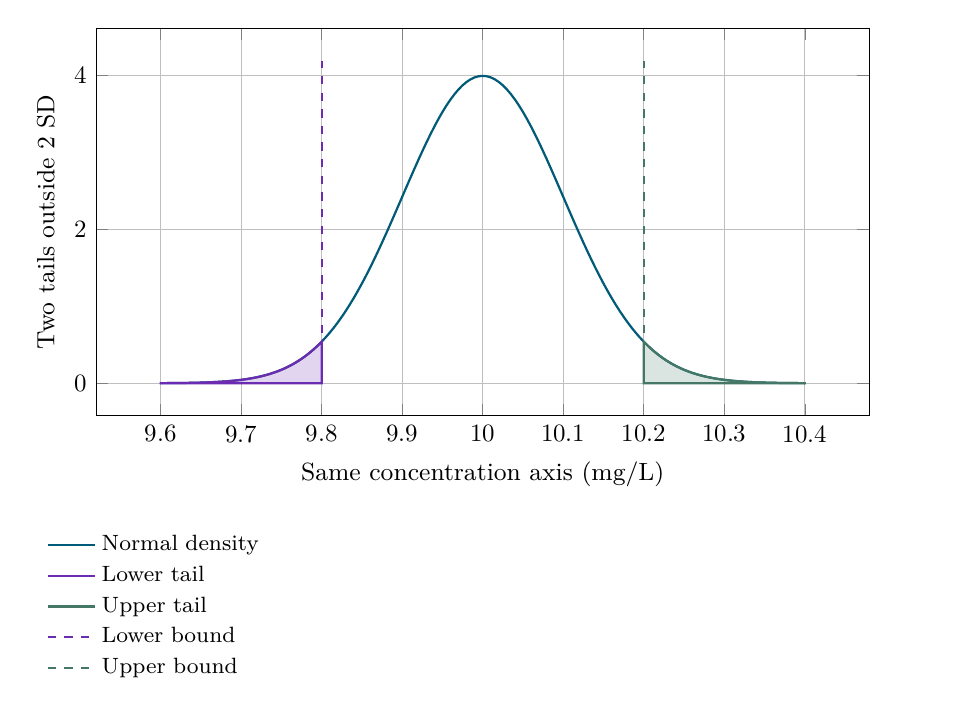
\begin{tikzpicture}
\begin{axis}[width=0.94\linewidth,
height=6.5cm,
scale only axis=false,
grid=major,
tick label style={font=\small},
label style={font=\small},
xlabel={Same concentration axis (mg/L)},
ylabel={Two tails outside 2 SD},
legend style={font=\footnotesize,draw=none,at={(0.5,-0.28)},anchor=north,legend columns=1,text width=0.85\linewidth,align=left},
unbounded coords=jump,
scaled ticks=false]
\addplot[color=pcd1,thick,mark=none] coordinates {(9.6,0.0013383022576488345) (9.605,0.0016325640876624478) (9.61,0.0019865547139276828) (9.615,0.002411265802259954) (9.62,0.002919469257914515) (9.625,0.0035259568236744544) (9.629999999999999,0.004247802705507359) (9.635,0.005104649743441814) (9.64,0.00611901930113785) (9.645,0.007316644628302992) (9.65,0.008726826950457709) (9.655,0.010382812956613882) (9.66,0.012322191684730253) (9.665,0.014587308046667044) (9.67,0.017225689390536765) (9.674999999999999,0.020290480572996972) (9.68,0.02384088201464821) (9.685,0.027942584148794893) (9.69,0.03266819056199869) (9.695,0.03809762098221841) (9.7,0.04431848411937913) (9.705,0.05142640923053953) (9.709999999999999,0.059525324197756954) (9.715,0.06872766690613948) (9.719999999999999,0.07915451582979711) (9.725,0.09093562501590964) (9.73,0.10420934814422717) (9.735,0.11912243607604998) (9.74,0.1358296923368569) (9.745,0.15449347134394867) (9.75,0.17528300493568538) (9.754999999999999,0.19837354391794843) (9.76,0.2239453029484278) (9.765,0.25218219915194723) (9.77,0.283270377416009) (9.775,0.31739651835667665) (9.78,0.35474592846230935) (9.785,0.39550041589370327) (9.79,0.4398359598042641) (9.795,0.4879201857918268) (9.8,0.5399096651318882) (9.805,0.5959470606881575) (9.81,0.6561581477467721) (9.815,0.7206487433621733) (9.82,0.7895015830089458) (9.825,0.8627731882651044) (9.83,0.9404907737688704) (9.834999999999999,1.0226492456397647) (9.84,1.109208346794553) (9.845,1.2000900069698677) (9.85,1.2951759566589105) (9.855,1.3943056644536114) (9.86,1.4972746563574368) (9.865,1.6038332734192007) (9.87,1.7136859204780563) (9.875,1.8264908538902191) (9.879999999999999,1.9418605498321064) (9.885,2.0593626871997426) (9.89,2.178521770325519) (9.895,2.2988214068423205) (9.9,2.419707245191442) (9.905,2.5405905646918745) (9.91,2.660852498987552) (9.915,2.7798488613099446) (9.92,2.896915527614826) (9.925,3.01137432154806) (9.93,3.1225393336676066) (9.935,3.2297235966791535) (9.94,3.3322460289179867) (9.945,3.4294385501938445) (9.95,3.5206532676429823) (9.955,3.605269624616481) (9.96,3.682701403033246) (9.965,3.7524034691693773) (9.97,3.8138781546052485) (9.975,3.8666811680284887) (9.98,3.9104269397545623) (9.985,3.944793309078886) (9.99,3.969525474770119) (9.995,3.9844391409476385) (10,3.989422804014327) (10.005,3.9844391409476385) (10.01,3.969525474770119) (10.015,3.944793309078886) (10.02,3.9104269397545623) (10.025,3.8666811680284887) (10.03,3.8138781546052485) (10.035,3.7524034691693773) (10.04,3.682701403033246) (10.045,3.605269624616481) (10.05,3.5206532676429823) (10.055,3.4294385501938445) (10.06,3.3322460289179867) (10.065,3.2297235966791535) (10.07,3.1225393336676066) (10.075,3.01137432154806) (10.08,2.896915527614826) (10.085,2.7798488613099446) (10.09,2.660852498987552) (10.095,2.5405905646918745) (10.1,2.419707245191442) (10.105,2.2988214068423205) (10.11,2.178521770325519) (10.115,2.0593626871997426) (10.120000000000001,1.9418605498321064) (10.125,1.8264908538902191) (10.13,1.7136859204780563) (10.135,1.6038332734192007) (10.14,1.4972746563574368) (10.145,1.3943056644536114) (10.15,1.2951759566589105) (10.155,1.2000900069698677) (10.16,1.109208346794553) (10.165000000000001,1.0226492456397647) (10.17,0.9404907737688704) (10.175,0.8627731882651044) (10.18,0.7895015830089458) (10.185,0.7206487433621733) (10.19,0.6561581477467721) (10.195,0.5959470606881575) (10.2,0.5399096651318882) (10.205,0.4879201857918268) (10.21,0.4398359598042641) (10.215,0.39550041589370327) (10.22,0.35474592846230935) (10.225,0.31739651835667665) (10.23,0.283270377416009) (10.235,0.25218219915194723) (10.24,0.2239453029484278) (10.245000000000001,0.19837354391794843) (10.25,0.17528300493568538) (10.255,0.15449347134394867) (10.26,0.1358296923368569) (10.265,0.11912243607604998) (10.27,0.10420934814422717) (10.275,0.09093562501590964) (10.280000000000001,0.07915451582979711) (10.285,0.06872766690613948) (10.290000000000001,0.059525324197756954) (10.295,0.05142640923053953) (10.3,0.04431848411937913) (10.305,0.03809762098221841) (10.31,0.03266819056199869) (10.315,0.027942584148794893) (10.32,0.02384088201464821) (10.325000000000001,0.020290480572996972) (10.33,0.017225689390536765) (10.335,0.014587308046667044) (10.34,0.012322191684730253) (10.345,0.010382812956613882) (10.35,0.008726826950457709) (10.355,0.007316644628302992) (10.36,0.00611901930113785) (10.365,0.005104649743441814) (10.370000000000001,0.004247802705507359) (10.375,0.0035259568236744544) (10.38,0.002919469257914515) (10.385,0.002411265802259954) (10.39,0.0019865547139276828) (10.395,0.0016325640876624478) (10.4,0.0013383022576488345)};
\addlegendentry{Normal density}
\addplot[color=pcd2,thick,mark=none,fill=pcd2,fill opacity=0.2] coordinates {(9.6,0.0013383022576488345) (9.60125,0.001406808570468116) (9.6025,0.0014785906029806861) (9.60375,0.001553792495532867) (9.605,0.0016325640876624478) (9.60625,0.0017150611119471863) (9.6075,0.0018014453929768815) (9.60875,0.0018918850515163626) (9.61,0.0019865547139276828) (9.61125,0.0020856357269142187) (9.612499999999999,0.0021893163776460296) (9.61375,0.0022977921193278205) (9.615,0.002411265802259954) (9.616249999999999,0.002529947910447312) (9.6175,0.002654056803802257) (9.61875,0.002783818965983658) (9.62,0.002919469257914515) (9.62125,0.003061251177011863) (9.6225,0.003209417122157465) (9.62375,0.0033642286644381416) (9.625,0.0035259568236744544) (9.62625,0.0036948823507502314) (9.6275,0.0038712960157558213) (9.62875,0.0040554989019461595) (9.629999999999999,0.004247802705507359) (9.63125,0.004448530041128044) (9.6325,0.004658014753350416) (9.63375,0.004876602233683178) (9.635,0.005104649743441814) (9.63625,0.005342526742273153) (9.6375,0.005590615222321504) (9.63875,0.0058493100479771395) (9.64,0.00611901930113785) (9.64125,0.006400164631914967) (9.6425,0.0066931816146965925) (9.64375,0.006998520109469603) (9.645,0.007316644628302992) (9.64625,0.007648034706874197) (9.647499999999999,0.007993185280907276) (9.64875,0.008352607067397287) (9.65,0.008726826950457709) (9.65125,0.009116388371642139) (9.6525,0.009521851724562653) (9.65375,0.009943794753613833) (9.655,0.010382812956613882) (9.65625,0.01083951999114652) (9.6575,0.011314548084372334) (9.65875,0.011808548446081594) (9.66,0.012322191684730253) (9.66125,0.012856168226184446) (9.6625,0.01341118873490361) (9.66375,0.013987984537259164) (9.665,0.014587308046667044) (9.66625,0.015209933190226317) (9.6675,0.01585665583649478) (9.66875,0.016528294224062184) (9.67,0.017225689390536765) (9.67125,0.017949705601542725) (9.6725,0.018701230779336154) (9.67375,0.019481176930604863) (9.675,0.02029048057299815) (9.67625,0.021130103159944628) (9.6775,0.02200103150327147) (9.67875,0.022904278193117432) (9.68,0.02384088201464821) (9.68125,0.024811908361033287) (9.6825,0.025818449642121537) (9.68375,0.026861625688283482) (9.685,0.027942584148794893) (9.68625,0.029062500884195035) (9.6875,0.030222580351987563) (9.68875,0.03142405598503175) (9.69,0.03266819056199869) (9.69125,0.033956276569207855) (9.6925,0.035289636553138465) (9.69375,0.03666962346294187) (9.695,0.03809762098221841) (9.696250000000001,0.0395750438493009) (9.6975,0.04110333816532535) (9.69875,0.04268398168930228) (9.7,0.04431848411937913) (9.70125,0.046008387359548056) (9.7025,0.04775526577091644) (9.70375,0.04956072640676641) (9.705,0.05142640923053953) (9.70625,0.053353987315864236) (9.7075,0.05534516702780428) (9.70875,0.05740168818442516) (9.71,0.05952532419776002) (9.71125,0.06171788219332329) (9.7125,0.06398120310723618) (9.713750000000001,0.06631716176001379) (9.715,0.06872766690613948) (9.71625,0.07121466125846662) (9.717500000000001,0.07378012148647028) (9.71875,0.07642605818746402) (9.72,0.07915451582980106) (9.72125,0.08196757266706482) (9.7225,0.08486734062238752) (9.72375,0.08785596514182238) (9.725,0.09093562501590964) (9.72625,0.09410853216844328) (9.727500000000001,0.09737693141144248) (9.72875,0.10074310016545712) (9.73,0.10420934814422717) (9.731250000000001,0.10777801700271208) (9.7325,0.11145147994764781) (9.73375,0.11523214130967137) (9.735000000000001,0.1191224360760556) (9.73625,0.12312482938325199) (9.7375,0.1272418159683167) (9.73875,0.13147591957829446) (9.74,0.1358296923368569) (9.74125,0.14030571406719194) (9.7425,0.1449065915704834) (9.74375,0.1496349578591408) (9.745000000000001,0.15449347134395566) (9.74625,0.15948481497456668) (9.7475,0.16461169533247474) (9.748750000000001,0.16987684167585976) (9.75,0.17528300493568538) (9.75125,0.180832956662417) (9.752500000000001,0.18652948792270502) (9.75375,0.19237540814563192) (9.755,0.19837354391795708) (9.75625,0.20452673772781213) (9.7575,0.2108378466566426) (9.758750000000001,0.21730974101876419) (9.76,0.2239453029484278) (9.76125,0.2307474249340283) (9.762500000000001,0.23771900829914405) (9.76375,0.2448629616303991) (9.765,0.25218219915194723) (9.766250000000001,0.2596796390464161) (9.7675,0.26735820172248276) (9.76875,0.27522080802904925) (9.770000000000001,0.28327037741602057) (9.77125,0.2915098260420593) (9.7725,0.29994206482945884) (9.77375,0.30856999746631714) (9.775,0.31739651835667665) (9.776250000000001,0.3264245105187122) (9.7775,0.3356568434317743) (9.77875,0.34509637083275885) (9.780000000000001,0.35474592846232317) (9.78125,0.3646083317619214) (9.7825,0.374686373522343) (9.783750000000001,0.38498282148450513) (9.785,0.39550041589370327) (9.78625,0.40624186700824017) (9.787500000000001,0.41720985256339865) (9.78875,0.4284070151922274) (9.790000000000001,0.4398359598042805) (9.791250000000002,0.4514992509235193) (9.7925,0.46339940998709644) (9.793750000000001,0.4755389126064066) (9.795,0.4879201857918268) (9.79625,0.5005456051432564) (9.797500000000001,0.513417492007707) (9.79875,0.526538110606222) (9.8,0.5399096651318882)} \closedcycle;
\addlegendentry{Lower tail}
\addplot[color=pcd3,thick,mark=none,fill=pcd3,fill opacity=0.2] coordinates {(10.2,0.5399096651318882) (10.20125,0.526538110606222) (10.202499999999999,0.513417492007707) (10.20375,0.5005456051432564) (10.205,0.4879201857918268) (10.206249999999999,0.4755389126064066) (10.2075,0.46339940998709644) (10.20875,0.4514992509235026) (10.209999999999999,0.4398359598042805) (10.21125,0.4284070151922274) (10.212499999999999,0.41720985256339865) (10.21375,0.40624186700824017) (10.215,0.39550041589370327) (10.216249999999999,0.38498282148450513) (10.2175,0.374686373522343) (10.21875,0.3646083317619214) (10.219999999999999,0.35474592846232317) (10.22125,0.34509637083275885) (10.2225,0.3356568434317743) (10.223749999999999,0.3264245105187122) (10.225,0.31739651835667665) (10.22625,0.30856999746631714) (10.2275,0.29994206482945884) (10.22875,0.2915098260420593) (10.229999999999999,0.28327037741602057) (10.23125,0.27522080802904925) (10.2325,0.26735820172248276) (10.233749999999999,0.2596796390464161) (10.235,0.25218219915194723) (10.23625,0.2448629616303991) (10.237499999999999,0.23771900829914405) (10.23875,0.2307474249340283) (10.24,0.2239453029484278) (10.241249999999999,0.21730974101876419) (10.2425,0.2108378466566426) (10.24375,0.20452673772781213) (10.245,0.19837354391795708) (10.24625,0.19237540814563192) (10.247499999999999,0.18652948792270502) (10.24875,0.180832956662417) (10.25,0.17528300493568538) (10.251249999999999,0.16987684167585976) (10.2525,0.16461169533247474) (10.25375,0.15948481497456668) (10.254999999999999,0.15449347134395566) (10.25625,0.1496349578591408) (10.2575,0.1449065915704834) (10.25875,0.14030571406719194) (10.26,0.1358296923368569) (10.26125,0.13147591957829446) (10.2625,0.1272418159683167) (10.26375,0.12312482938325199) (10.264999999999999,0.1191224360760556) (10.26625,0.11523214130967137) (10.2675,0.11145147994764781) (10.268749999999999,0.10777801700271208) (10.27,0.10420934814422717) (10.27125,0.10074310016545712) (10.272499999999999,0.09737693141144248) (10.27375,0.09410853216844328) (10.275,0.09093562501590964) (10.27625,0.08785596514182238) (10.2775,0.08486734062238752) (10.27875,0.08196757266706482) (10.28,0.07915451582980106) (10.28125,0.07642605818746402) (10.282499999999999,0.07378012148647028) (10.28375,0.07121466125846662) (10.285,0.06872766690613948) (10.286249999999999,0.06631716176001379) (10.2875,0.06398120310723618) (10.28875,0.06171788219332329) (10.29,0.05952532419776002) (10.29125,0.05740168818442516) (10.2925,0.05534516702780428) (10.29375,0.053353987315864236) (10.295,0.05142640923053953) (10.29625,0.04956072640676641) (10.2975,0.04775526577091644) (10.29875,0.046008387359548056) (10.3,0.04431848411937913) (10.30125,0.04268398168930228) (10.3025,0.04110333816532535) (10.303749999999999,0.0395750438493009) (10.305,0.03809762098221841) (10.30625,0.03666962346294187) (10.3075,0.035289636553138465) (10.30875,0.033956276569207855) (10.31,0.03266819056199869) (10.31125,0.03142405598503175) (10.3125,0.030222580351987563) (10.31375,0.029062500884195035) (10.315,0.027942584148794893) (10.31625,0.026861625688283482) (10.3175,0.025818449642121537) (10.31875,0.024811908361033287) (10.32,0.02384088201464821) (10.32125,0.022904278193117432) (10.3225,0.02200103150327147) (10.32375,0.021130103159944628) (10.325,0.02029048057299815) (10.32625,0.019481176930604863) (10.3275,0.018701230779336154) (10.32875,0.017949705601542725) (10.33,0.017225689390536765) (10.33125,0.016528294224062184) (10.3325,0.01585665583649478) (10.33375,0.015209933190226317) (10.335,0.014587308046667044) (10.33625,0.013987984537259164) (10.3375,0.01341118873490361) (10.33875,0.012856168226184446) (10.34,0.012322191684730253) (10.34125,0.011808548446081594) (10.3425,0.011314548084372334) (10.34375,0.01083951999114652) (10.345,0.010382812956613882) (10.34625,0.009943794753613833) (10.3475,0.009521851724562653) (10.34875,0.009116388371642139) (10.35,0.008726826950457709) (10.35125,0.008352607067397287) (10.352500000000001,0.007993185280907276) (10.35375,0.007648034706874197) (10.355,0.007316644628302992) (10.35625,0.006998520109469603) (10.3575,0.0066931816146965925) (10.35875,0.006400164631914967) (10.36,0.00611901930113785) (10.36125,0.0058493100479771395) (10.3625,0.005590615222321504) (10.36375,0.005342526742273153) (10.365,0.005104649743441814) (10.36625,0.004876602233683178) (10.3675,0.004658014753350416) (10.36875,0.004448530041128044) (10.370000000000001,0.004247802705507359) (10.37125,0.0040554989019461595) (10.3725,0.0038712960157558213) (10.37375,0.0036948823507502314) (10.375,0.0035259568236744544) (10.37625,0.0033642286644381416) (10.3775,0.003209417122157465) (10.37875,0.003061251177011863) (10.38,0.002919469257914515) (10.38125,0.002783818965983658) (10.3825,0.002654056803802257) (10.383750000000001,0.002529947910447312) (10.385,0.002411265802259954) (10.38625,0.0022977921193278205) (10.387500000000001,0.0021893163776460296) (10.38875,0.0020856357269142187) (10.39,0.0019865547139276828) (10.39125,0.0018918850515163626) (10.3925,0.0018014453929768815) (10.39375,0.0017150611119471863) (10.395,0.0016325640876624478) (10.39625,0.001553792495532867) (10.3975,0.0014785906029806861) (10.39875,0.001406808570468116) (10.4,0.0013383022576488345)} \closedcycle;
\addlegendentry{Upper tail}
\addplot[color=pcd2,dashed,thick] coordinates {(9.8,0) (9.8,4.188893944215043)};
\addlegendentry{Lower bound}
\addplot[color=pcd3,dashed,thick] coordinates {(10.2,0) (10.2,4.188893944215043)};
\addlegendentry{Upper bound}
\end{axis}
\end{tikzpicture}
\end{center}

% Full-precision experiment details: {"blockId":"ex:p1-n18-v--block","parameters":[{"key":"sigma","label":"True method SD (mg/L), assumed","value":0.1},{"key":"mu","label":"Assumed method expectation (mg/L)","value":10},{"key":"threshold","label":"Chosen threshold (mg/L)","value":10.2},{"key":"alpha","label":"Chosen upper-tail rate","value":0.01},{"key":"inverse","label":"Inverse mode: upper rate chosen first","value":1},{"key":"band","label":"Symmetric distance in SD units","value":2},{"key":"view","label":"Authored inverse / interval view","value":3}],"readouts":[{"label":"Threshold","value":10.232634787404084},{"label":"Standardized distance","value":2.3263478740408416},{"label":"Standard-normal density at distance","value":0.026652142203458018},{"label":"Left probability","value":0.99},{"label":"Upper probability","value":0.009999999999999976},{"label":"Central coverage","value":0.9544997361036418},{"label":"Total outside both bounds","value":0.045500263896358195}],"note":"Probabilities are areas under the density over the full model domain. The displayed examples use explicitly specified model parameters. A one-sided upper rate and the total outside a symmetric band are different events.","markers":[[{"x":10.232634787404084,"label":"Selected quantile"}],[{"x":9.8,"label":"Lower bound"},{"x":10.2,"label":"Upper bound"}]]}

\medskip

The density in \hyperref[material-a53119fde01e4c7d3d126fca644fc3014e28b2cfcf43b6b61bc9ecd1bef631a9]{Eq.~\ref*{material-a53119fde01e4c7d3d126fca644fc3014e28b2cfcf43b6b61bc9ecd1bef631a9}} and standardization in \hyperref[material-71c7f58d4d53a93a0fff415857fac2987d4bf2e4b685d9577271097873cffcc1]{Eq.~\ref*{material-71c7f58d4d53a93a0fff415857fac2987d4bf2e4b685d9577271097873cffcc1}} supply the common reference. Applying it to two specified model spreads in \hyperref[material-819b81fd4211b44ecc9ada2ba22ddea5b27cb37dfae01bcf3648df617e78576e]{Eq.~\ref*{material-819b81fd4211b44ecc9ada2ba22ddea5b27cb37dfae01bcf3648df617e78576e}} gives different standardized distances for a common concentration. The CDF identity in \hyperref[material-d2421efb8efa48f57f0ac23eab8293e26bfec08fca8e196b7d2fed2bd1ef2220]{Eq.~\ref*{material-d2421efb8efa48f57f0ac23eab8293e26bfec08fca8e196b7d2fed2bd1ef2220}} leads to the upper-tail calculation in \hyperref[material-804e7fe955d16abfdf9a5d60c17185ecc503bb8db2a8ee3183aadb930cca4cf6]{Eq.~\ref*{material-804e7fe955d16abfdf9a5d60c17185ecc503bb8db2a8ee3183aadb930cca4cf6}}, while \hyperref[material-9a7e53ed52e0b40a301aceb066b4784f8177c258b1203d04817112526a0ed6ec]{Eq.~\ref*{material-9a7e53ed52e0b40a301aceb066b4784f8177c258b1203d04817112526a0ed6ec}} gives central band coverage. A one-sided limit and a central band answer different analytical questions even when they use the same model (\hyperref[material-595c2eaec5967f0cf95d21867b5811806843dc62dbed1eacc46ed098c4201128]{Fig.~\ref*{material-595c2eaec5967f0cf95d21867b5811806843dc62dbed1eacc46ed098c4201128}}). The optional source in \hyperref[material-1095cbe806ce6a89cdd8c58f223c6f8d8423553f96457954efa3e34898b21b68]{Listing~\ref*{material-1095cbe806ce6a89cdd8c58f223c6f8d8423553f96457954efa3e34898b21b68}} makes the probabilities and limits reproducible in R.


\par\medskip
\noindent\begin{minipage}{\linewidth}
\refstepcounter{equation}\label{material-a53119fde01e4c7d3d126fca644fc3014e28b2cfcf43b6b61bc9ecd1bef631a9}
\noindent\textbf{Eq.~\ref*{material-a53119fde01e4c7d3d126fca644fc3014e28b2cfcf43b6b61bc9ecd1bef631a9}.} The standard-Normal density \(\varphi\) as a function of standardized distance.\par\nopagebreak
\begin{center}\begin{adjustbox}{max width=\linewidth}$\displaystyle \varphi(z)=\frac{1}{\sqrt{2\pi}}e^{-z^2/2}$\end{adjustbox}\end{center}

\par\noindent\textbf{Symbols}

\begin{itemize}\setlength{\itemsep}{1pt}\setlength{\parsep}{0pt}
\item \textbf{\ensuremath{\varphi}(z)}: Standard-normal density per dimensionless z-unit.
\item \textbf{z}: Concrete standardized value, in SD units.
\item \textbf{e}: Base of the natural exponential.
\item \textbf{\ensuremath{\pi}}: Circle constant.
\item \textbf{z\ensuremath{{}^2}, \ensuremath{-}, /}: Square z, negate it and divide by two in the exponent.
\item \textbf{\ensuremath{\sqrt{\vphantom{x}}}(2\ensuremath{\pi})}: Positive square root of two times \ensuremath{\pi}; the density's normalizing denominator.
\item \textbf{=}: Equality defining the density.
\end{itemize}

The density is symmetric around zero, where it is maximal, and has total area one. Probabilities are areas over intervals.

\end{minipage}\par
\medskip

\par\medskip
\noindent\begin{minipage}{\linewidth}
\refstepcounter{equation}\label{material-71c7f58d4d53a93a0fff415857fac2987d4bf2e4b685d9577271097873cffcc1}
\noindent\textbf{Eq.~\ref*{material-71c7f58d4d53a93a0fff415857fac2987d4bf2e4b685d9577271097873cffcc1}.} Normal measurement results expressed through location, scale and standardized distance.\par\nopagebreak
\begin{center}\begin{adjustbox}{max width=\linewidth}$\displaystyle \begin{gathered}X\sim\mathcal N(\mu,\sigma^2),\quad Z=\frac{X-\mu}{\sigma}\sim\mathcal N(0,1)\\z=\frac{x-\mu}{\sigma}=\frac{10.20-10.00}{0.10}=2\end{gathered}$\end{adjustbox}\end{center}

\par\noindent\textbf{Symbols}

\begin{itemize}\setlength{\itemsep}{1pt}\setlength{\parsep}{0pt}
\item \textbf{X}: Random nitrate concentration (mg/L).
\item \textbf{x}: Concrete result, 10.20 mg/L.
\item \textbf{\ensuremath{\mu}}: Known model expectation, 10.00 mg/L.
\item \textbf{\ensuremath{\sigma}}: Known positive model SD, 0.10 mg/L.
\item \textbf{\ensuremath{\sigma}\ensuremath{{}^2}}: Model variance ((mg/L)\ensuremath{{}^2}).
\item \textbf{Z}: Standardized random variable, with mean zero and variance one under the Normal model.
\item \textbf{z}: Concrete standardized distance, 2 here (dimensionless).
\item \textbf{N, \ensuremath{\sim}}: Normal distribution, parameterized by mean and variance; follows that distribution.
\item \textbf{\ensuremath{-}, /, \ensuremath{{}^2}, =}: Subtraction, division, squaring and equality defining or evaluating a value.
\end{itemize}

Subtracting \ensuremath{\mu} and dividing by \ensuremath{\sigma} cancels concentration units. Standardization preserves distributional shape; a standard-normal reference requires a Normal starting model.

\end{minipage}\par
\medskip

\par\medskip
\noindent\begin{minipage}{\linewidth}
\refstepcounter{equation}\label{material-819b81fd4211b44ecc9ada2ba22ddea5b27cb37dfae01bcf3648df617e78576e}
\noindent\textbf{Eq.~\ref*{material-819b81fd4211b44ecc9ada2ba22ddea5b27cb37dfae01bcf3648df617e78576e}.} Standardizing a common concentration with two specified model standard deviations.\par\nopagebreak
\begin{center}\begin{adjustbox}{max width=\linewidth}$\displaystyle \begin{gathered}z_A=\frac{10.20-10.00}{0.10}=2\\z_B=\frac{10.20-10.00}{0.20}=1\end{gathered}$\end{adjustbox}\end{center}

\par\noindent\textbf{Symbols}

\begin{itemize}\setlength{\itemsep}{1pt}\setlength{\parsep}{0pt}
\item \textbf{\(z_A\)}: Standardized distance for method A, equal to 2 (dimensionless).
\item \textbf{\(z_B\)}: Standardized distance for method B, equal to 1 (dimensionless).
\item \textbf{A, B}: Method-identifying subscripts.
\item \textbf{\ensuremath{-}, /, =}: Subtract expectation, divide by that method's SD, and evaluate the distance.
\end{itemize}

Both Normal models have known expectation 10.00 mg/L and result 10.20 mg/L. Their known SDs are 0.10 mg/L for A and 0.20 mg/L for B; concentration units cancel in each ratio.

\end{minipage}\par
\medskip

\par\medskip
\noindent\begin{minipage}{\linewidth}
\refstepcounter{equation}\label{material-d2421efb8efa48f57f0ac23eab8293e26bfec08fca8e196b7d2fed2bd1ef2220}
\noindent\textbf{Eq.~\ref*{material-d2421efb8efa48f57f0ac23eab8293e26bfec08fca8e196b7d2fed2bd1ef2220}.} The standard-Normal CDF \(\Phi\) and its error-function representation.\par\nopagebreak
\begin{center}\begin{adjustbox}{max width=\linewidth}$\displaystyle \begin{gathered}\Phi(z)=P(Z\le z)\\=\int_{-\infty}^{z}\varphi(t)\,dt\\=\frac12\left[1+\operatorname{erf}\!\left(\frac{z}{\sqrt2}\right)\right]\\\operatorname{erf}(u)=\frac{2}{\sqrt\pi}\int_0^u e^{-t^2}\,dt\\\Phi(2)\approx0.9772499\end{gathered}$\end{adjustbox}\end{center}

\par\noindent\textbf{Symbols}

\begin{itemize}\setlength{\itemsep}{1pt}\setlength{\parsep}{0pt}
\item \textbf{\ensuremath{\Phi}(z)}: Standard-normal cumulative probability at z; a special case of F.
\item \textbf{\ensuremath{\varphi}(t)}: Standard-normal density at t; a special case of f.
\item \textbf{Z}: Standard-normal random variable.
\item \textbf{z}: Concrete standardized threshold, 2 here (dimensionless).
\item \textbf{t}: Dimensionless integration variable.
\item \textbf{P, \ensuremath{\le}}: Probability; at or below the threshold.
\item \textbf{\ensuremath{\int}, \ensuremath{-}\ensuremath{\infty}, dt}: Integrate from minus infinity up to z; dt is the increment of t.
\item \textbf{=, \ensuremath{\approx}}: Equality and approximate equality.
\end{itemize}

The CDF slope equals the density where the derivative exists. All quantities use the standardized, dimensionless scale.

\begin{itemize}\setlength{\itemsep}{1pt}\setlength{\parsep}{0pt}
\item \textbf{erf(u)}: Error function at dimensionless argument u.
\item \textbf{u}: Upper integration limit in the definition of erf.
\item \textbf{t, dt}: Dimensionless integration variable and its infinitesimal increment.
\item \textbf{\ensuremath{\int}\ensuremath{{}_0}\ensuremath{{}^u}}: Integrate from zero to u.
\item \textbf{e\ensuremath{{}^-}\ensuremath{{}^t}\ensuremath{{}^2}}: Natural exponential with exponent \ensuremath{-}t\ensuremath{{}^2}.
\item \textbf{\ensuremath{\pi}}: Circle constant.
\item \textbf{\ensuremath{\sqrt{\vphantom{x}}}}: Positive square root.
\item \textbf{2 / \ensuremath{\sqrt{\vphantom{x}}}\ensuremath{\pi}}: Normalizing factor in the definition of erf.
\item \textbf{z / \ensuremath{\sqrt{\vphantom{x}}}2}: Scaled standardized threshold used as the erf argument.
\item \textbf{\ensuremath{\tfrac12}, 1, +}: Multiply the grouped expression by one half after adding one.
\item \textbf{( ), [ ]}: Group the stated operations.
\end{itemize}

All quantities here are dimensionless. The error function erf provides the special-function representation of the standard-normal density's antiderivative. Integrating from minus infinity fixes the CDF normalization.

\end{minipage}\par
\medskip

\par\medskip
\noindent\begin{minipage}{\linewidth}
\refstepcounter{equation}\label{material-804e7fe955d16abfdf9a5d60c17185ecc503bb8db2a8ee3183aadb930cca4cf6}
\noindent\textbf{Eq.~\ref*{material-804e7fe955d16abfdf9a5d60c17185ecc503bb8db2a8ee3183aadb930cca4cf6}.} Upper-tail probability for a fixed concentration limit under a known Normal model.\par\nopagebreak
\begin{center}\begin{adjustbox}{max width=\linewidth}$\displaystyle \begin{gathered}\varphi(2)\approx0.05399\\P(X>10.20)=1-\Phi(2)\\\approx0.02275\end{gathered}$\end{adjustbox}\end{center}

\par\noindent\textbf{Symbols}

\begin{itemize}\setlength{\itemsep}{1pt}\setlength{\parsep}{0pt}
\item \textbf{X}: Normal random concentration (mg/L), with mean 10.00 mg/L and SD 0.10 mg/L.
\item \textbf{z}: Standardized threshold, 2 at concentration 10.20 mg/L.
\item \textbf{\ensuremath{\varphi}(2)}: Density at z = 2, per dimensionless z-unit.
\item \textbf{\ensuremath{\Phi}(2)}: Cumulative probability at z = 2.
\item \textbf{P, >}: Probability of exceeding the stated threshold.
\item \textbf{\ensuremath{-}, /, =, \ensuremath{\approx}}: Subtraction, division, equality and approximate equality.
\end{itemize}

Subtracting \ensuremath{\Phi}(2) from total probability one gives the upper-tail probability, about 2.275\%.

\end{minipage}\par
\medskip

\par\medskip
\noindent\begin{minipage}{\linewidth}
\refstepcounter{equation}\label{material-9a7e53ed52e0b40a301aceb066b4784f8177c258b1203d04817112526a0ed6ec}
\noindent\textbf{Eq.~\ref*{material-9a7e53ed52e0b40a301aceb066b4784f8177c258b1203d04817112526a0ed6ec}.} Normal-model probability within one, two and three standard deviations of the mean.\par\nopagebreak
\begin{center}\begin{adjustbox}{max width=\linewidth}$\displaystyle \begin{gathered}P(a\le Z\le b)=\Phi(b)-\Phi(a)\\P(-k\le Z\le k)=2\Phi(k)-1\end{gathered}$\end{adjustbox}\end{center}

\par\noindent\textbf{Symbols}

\begin{itemize}\setlength{\itemsep}{1pt}\setlength{\parsep}{0pt}
\item \textbf{Z}: Standard-normal random variable.
\item \textbf{a, b}: Ordered interval bounds (dimensionless).
\item \textbf{k}: Positive symmetric distance from zero, in SD units.
\item \textbf{P}: Probability.
\item \textbf{\ensuremath{\Phi}}: Standard-normal CDF, giving cumulative probability.
\item \textbf{\ensuremath{\le}}: Includes each interval endpoint; each exact value has probability zero.
\item \textbf{\ensuremath{-}, +, =}: Subtraction, addition and equality.
\item \textbf{2\ensuremath{\Phi}(k)}: Two times \ensuremath{\Phi}(k); adjacent quantities multiply.
\end{itemize}

Subtract the lower CDF from the upper. Symmetry gives central coverage 2\ensuremath{\Phi}(k) \ensuremath{-} 1, leaving one tail on each side.

\end{minipage}\par
\medskip

\par\medskip
\Needspace{10cm}
\refstepcounter{figure}\label{material-595c2eaec5967f0cf95d21867b5811806843dc62dbed1eacc46ed098c4201128}
\noindent\textbf{Fig.~\ref*{material-595c2eaec5967f0cf95d21867b5811806843dc62dbed1eacc46ed098c4201128}.} The shaded area lies above 10.20 mg/L, two SD above the expectation, in a Normal model with expectation 10.00 mg/L and SD 0.10 mg/L. It contains about 2.275\% of the model probability; about 97.72\% lies at or below the limit.\par\nopagebreak
\begin{center}
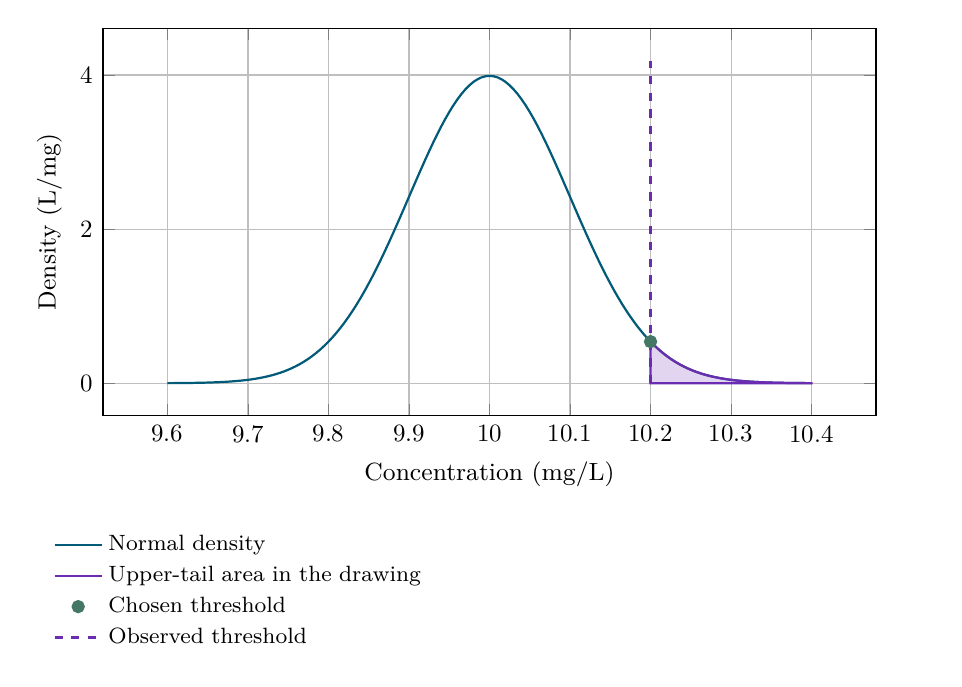
\begin{tikzpicture}
\begin{axis}[width=0.94\linewidth,
height=6.5cm,
scale only axis=false,
grid=major,
tick label style={font=\small},
label style={font=\small},
xlabel={Concentration (mg/L)},
ylabel={Density (L/mg)},
legend style={font=\footnotesize,draw=none,at={(0.5,-0.28)},anchor=north,legend columns=1,text width=0.85\linewidth,align=left},
unbounded coords=jump,
scaled ticks=false]
\addplot[color=pcd1,thick,mark=none] coordinates {(9.6,0.0013383022576488345) (9.605,0.0016325640876624478) (9.61,0.0019865547139276828) (9.615,0.002411265802259954) (9.62,0.002919469257914515) (9.625,0.0035259568236744544) (9.629999999999999,0.004247802705507359) (9.635,0.005104649743441814) (9.64,0.00611901930113785) (9.645,0.007316644628302992) (9.65,0.008726826950457709) (9.655,0.010382812956613882) (9.66,0.012322191684730253) (9.665,0.014587308046667044) (9.67,0.017225689390536765) (9.674999999999999,0.020290480572996972) (9.68,0.02384088201464821) (9.685,0.027942584148794893) (9.69,0.03266819056199869) (9.695,0.03809762098221841) (9.7,0.04431848411937913) (9.705,0.05142640923053953) (9.709999999999999,0.059525324197756954) (9.715,0.06872766690613948) (9.719999999999999,0.07915451582979711) (9.725,0.09093562501590964) (9.73,0.10420934814422717) (9.735,0.11912243607604998) (9.74,0.1358296923368569) (9.745,0.15449347134394867) (9.75,0.17528300493568538) (9.754999999999999,0.19837354391794843) (9.76,0.2239453029484278) (9.765,0.25218219915194723) (9.77,0.283270377416009) (9.775,0.31739651835667665) (9.78,0.35474592846230935) (9.785,0.39550041589370327) (9.79,0.4398359598042641) (9.795,0.4879201857918268) (9.8,0.5399096651318882) (9.805,0.5959470606881575) (9.81,0.6561581477467721) (9.815,0.7206487433621733) (9.82,0.7895015830089458) (9.825,0.8627731882651044) (9.83,0.9404907737688704) (9.834999999999999,1.0226492456397647) (9.84,1.109208346794553) (9.845,1.2000900069698677) (9.85,1.2951759566589105) (9.855,1.3943056644536114) (9.86,1.4972746563574368) (9.865,1.6038332734192007) (9.87,1.7136859204780563) (9.875,1.8264908538902191) (9.879999999999999,1.9418605498321064) (9.885,2.0593626871997426) (9.89,2.178521770325519) (9.895,2.2988214068423205) (9.9,2.419707245191442) (9.905,2.5405905646918745) (9.91,2.660852498987552) (9.915,2.7798488613099446) (9.92,2.896915527614826) (9.925,3.01137432154806) (9.93,3.1225393336676066) (9.935,3.2297235966791535) (9.94,3.3322460289179867) (9.945,3.4294385501938445) (9.95,3.5206532676429823) (9.955,3.605269624616481) (9.96,3.682701403033246) (9.965,3.7524034691693773) (9.97,3.8138781546052485) (9.975,3.8666811680284887) (9.98,3.9104269397545623) (9.985,3.944793309078886) (9.99,3.969525474770119) (9.995,3.9844391409476385) (10,3.989422804014327) (10.005,3.9844391409476385) (10.01,3.969525474770119) (10.015,3.944793309078886) (10.02,3.9104269397545623) (10.025,3.8666811680284887) (10.03,3.8138781546052485) (10.035,3.7524034691693773) (10.04,3.682701403033246) (10.045,3.605269624616481) (10.05,3.5206532676429823) (10.055,3.4294385501938445) (10.06,3.3322460289179867) (10.065,3.2297235966791535) (10.07,3.1225393336676066) (10.075,3.01137432154806) (10.08,2.896915527614826) (10.085,2.7798488613099446) (10.09,2.660852498987552) (10.095,2.5405905646918745) (10.1,2.419707245191442) (10.105,2.2988214068423205) (10.11,2.178521770325519) (10.115,2.0593626871997426) (10.120000000000001,1.9418605498321064) (10.125,1.8264908538902191) (10.13,1.7136859204780563) (10.135,1.6038332734192007) (10.14,1.4972746563574368) (10.145,1.3943056644536114) (10.15,1.2951759566589105) (10.155,1.2000900069698677) (10.16,1.109208346794553) (10.165000000000001,1.0226492456397647) (10.17,0.9404907737688704) (10.175,0.8627731882651044) (10.18,0.7895015830089458) (10.185,0.7206487433621733) (10.19,0.6561581477467721) (10.195,0.5959470606881575) (10.2,0.5399096651318882) (10.205,0.4879201857918268) (10.21,0.4398359598042641) (10.215,0.39550041589370327) (10.22,0.35474592846230935) (10.225,0.31739651835667665) (10.23,0.283270377416009) (10.235,0.25218219915194723) (10.24,0.2239453029484278) (10.245000000000001,0.19837354391794843) (10.25,0.17528300493568538) (10.255,0.15449347134394867) (10.26,0.1358296923368569) (10.265,0.11912243607604998) (10.27,0.10420934814422717) (10.275,0.09093562501590964) (10.280000000000001,0.07915451582979711) (10.285,0.06872766690613948) (10.290000000000001,0.059525324197756954) (10.295,0.05142640923053953) (10.3,0.04431848411937913) (10.305,0.03809762098221841) (10.31,0.03266819056199869) (10.315,0.027942584148794893) (10.32,0.02384088201464821) (10.325000000000001,0.020290480572996972) (10.33,0.017225689390536765) (10.335,0.014587308046667044) (10.34,0.012322191684730253) (10.345,0.010382812956613882) (10.35,0.008726826950457709) (10.355,0.007316644628302992) (10.36,0.00611901930113785) (10.365,0.005104649743441814) (10.370000000000001,0.004247802705507359) (10.375,0.0035259568236744544) (10.38,0.002919469257914515) (10.385,0.002411265802259954) (10.39,0.0019865547139276828) (10.395,0.0016325640876624478) (10.4,0.0013383022576488345)};
\addlegendentry{Normal density}
\addplot[color=pcd2,thick,mark=none,fill=pcd2,fill opacity=0.2] coordinates {(10.2,0.5399096651318882) (10.20125,0.526538110606222) (10.202499999999999,0.513417492007707) (10.20375,0.5005456051432564) (10.205,0.4879201857918268) (10.206249999999999,0.4755389126064066) (10.2075,0.46339940998709644) (10.20875,0.4514992509235026) (10.209999999999999,0.4398359598042805) (10.21125,0.4284070151922274) (10.212499999999999,0.41720985256339865) (10.21375,0.40624186700824017) (10.215,0.39550041589370327) (10.216249999999999,0.38498282148450513) (10.2175,0.374686373522343) (10.21875,0.3646083317619214) (10.219999999999999,0.35474592846232317) (10.22125,0.34509637083275885) (10.2225,0.3356568434317743) (10.223749999999999,0.3264245105187122) (10.225,0.31739651835667665) (10.22625,0.30856999746631714) (10.2275,0.29994206482945884) (10.22875,0.2915098260420593) (10.229999999999999,0.28327037741602057) (10.23125,0.27522080802904925) (10.2325,0.26735820172248276) (10.233749999999999,0.2596796390464161) (10.235,0.25218219915194723) (10.23625,0.2448629616303991) (10.237499999999999,0.23771900829914405) (10.23875,0.2307474249340283) (10.24,0.2239453029484278) (10.241249999999999,0.21730974101876419) (10.2425,0.2108378466566426) (10.24375,0.20452673772781213) (10.245,0.19837354391795708) (10.24625,0.19237540814563192) (10.247499999999999,0.18652948792270502) (10.24875,0.180832956662417) (10.25,0.17528300493568538) (10.251249999999999,0.16987684167585976) (10.2525,0.16461169533247474) (10.25375,0.15948481497456668) (10.254999999999999,0.15449347134395566) (10.25625,0.1496349578591408) (10.2575,0.1449065915704834) (10.25875,0.14030571406719194) (10.26,0.1358296923368569) (10.26125,0.13147591957829446) (10.2625,0.1272418159683167) (10.26375,0.12312482938325199) (10.264999999999999,0.1191224360760556) (10.26625,0.11523214130967137) (10.2675,0.11145147994764781) (10.268749999999999,0.10777801700271208) (10.27,0.10420934814422717) (10.27125,0.10074310016545712) (10.272499999999999,0.09737693141144248) (10.27375,0.09410853216844328) (10.275,0.09093562501590964) (10.27625,0.08785596514182238) (10.2775,0.08486734062238752) (10.27875,0.08196757266706482) (10.28,0.07915451582980106) (10.28125,0.07642605818746402) (10.282499999999999,0.07378012148647028) (10.28375,0.07121466125846662) (10.285,0.06872766690613948) (10.286249999999999,0.06631716176001379) (10.2875,0.06398120310723618) (10.28875,0.06171788219332329) (10.29,0.05952532419776002) (10.29125,0.05740168818442516) (10.2925,0.05534516702780428) (10.29375,0.053353987315864236) (10.295,0.05142640923053953) (10.29625,0.04956072640676641) (10.2975,0.04775526577091644) (10.29875,0.046008387359548056) (10.3,0.04431848411937913) (10.30125,0.04268398168930228) (10.3025,0.04110333816532535) (10.303749999999999,0.0395750438493009) (10.305,0.03809762098221841) (10.30625,0.03666962346294187) (10.3075,0.035289636553138465) (10.30875,0.033956276569207855) (10.31,0.03266819056199869) (10.31125,0.03142405598503175) (10.3125,0.030222580351987563) (10.31375,0.029062500884195035) (10.315,0.027942584148794893) (10.31625,0.026861625688283482) (10.3175,0.025818449642121537) (10.31875,0.024811908361033287) (10.32,0.02384088201464821) (10.32125,0.022904278193117432) (10.3225,0.02200103150327147) (10.32375,0.021130103159944628) (10.325,0.02029048057299815) (10.32625,0.019481176930604863) (10.3275,0.018701230779336154) (10.32875,0.017949705601542725) (10.33,0.017225689390536765) (10.33125,0.016528294224062184) (10.3325,0.01585665583649478) (10.33375,0.015209933190226317) (10.335,0.014587308046667044) (10.33625,0.013987984537259164) (10.3375,0.01341118873490361) (10.33875,0.012856168226184446) (10.34,0.012322191684730253) (10.34125,0.011808548446081594) (10.3425,0.011314548084372334) (10.34375,0.01083951999114652) (10.345,0.010382812956613882) (10.34625,0.009943794753613833) (10.3475,0.009521851724562653) (10.34875,0.009116388371642139) (10.35,0.008726826950457709) (10.35125,0.008352607067397287) (10.352500000000001,0.007993185280907276) (10.35375,0.007648034706874197) (10.355,0.007316644628302992) (10.35625,0.006998520109469603) (10.3575,0.0066931816146965925) (10.35875,0.006400164631914967) (10.36,0.00611901930113785) (10.36125,0.0058493100479771395) (10.3625,0.005590615222321504) (10.36375,0.005342526742273153) (10.365,0.005104649743441814) (10.36625,0.004876602233683178) (10.3675,0.004658014753350416) (10.36875,0.004448530041128044) (10.370000000000001,0.004247802705507359) (10.37125,0.0040554989019461595) (10.3725,0.0038712960157558213) (10.37375,0.0036948823507502314) (10.375,0.0035259568236744544) (10.37625,0.0033642286644381416) (10.3775,0.003209417122157465) (10.37875,0.003061251177011863) (10.38,0.002919469257914515) (10.38125,0.002783818965983658) (10.3825,0.002654056803802257) (10.383750000000001,0.002529947910447312) (10.385,0.002411265802259954) (10.38625,0.0022977921193278205) (10.387500000000001,0.0021893163776460296) (10.38875,0.0020856357269142187) (10.39,0.0019865547139276828) (10.39125,0.0018918850515163626) (10.3925,0.0018014453929768815) (10.39375,0.0017150611119471863) (10.395,0.0016325640876624478) (10.39625,0.001553792495532867) (10.3975,0.0014785906029806861) (10.39875,0.001406808570468116) (10.4,0.0013383022576488345)} \closedcycle;
\addlegendentry{Upper-tail area in the drawing}
\addplot[color=pcd3,thick,only marks,mark=*] coordinates {(10.2,0.5399096651318882)};
\addlegendentry{Chosen threshold}
\addplot[color=pcd2,dashed,thick] coordinates {(10.2,0) (10.2,4.188893944215043)};
\addlegendentry{Observed threshold}
\end{axis}
\end{tikzpicture}
\end{center}

% Full-precision experiment details: {"blockId":"ex:p1-n15-v--block","parameters":[{"key":"sigma","label":"True method SD (mg/L), assumed","value":0.1},{"key":"mu","label":"Assumed method expectation (mg/L)","value":10},{"key":"threshold","label":"Chosen threshold (mg/L)","value":10.2},{"key":"alpha","label":"Chosen upper-tail rate","value":0.01},{"key":"inverse","label":"Inverse mode: 0 threshold, 1 rate","value":0},{"key":"view","label":"Authored focused / decision view","value":2}],"readouts":[{"label":"Threshold","value":10.2},{"label":"Standardized distance","value":1.999999999999993},{"label":"Left probability","value":0.9772498680518206},{"label":"Upper probability","value":0.02275013194817947}],"note":"Probabilities are areas under the density over the full model domain. The displayed examples use explicitly specified model parameters. Inverse mode selects an upper-tail rate before inspecting data.","markers":[[{"x":10.2,"label":"Observed threshold"}]]}

\medskip

\par\medskip
\Needspace{8\baselineskip}
\refstepcounter{listing}\label{material-1095cbe806ce6a89cdd8c58f223c6f8d8423553f96457954efa3e34898b21b68}
\noindent\textbf{Listing~\ref*{material-1095cbe806ce6a89cdd8c58f223c6f8d8423553f96457954efa3e34898b21b68}.} R calculations of known-model Normal tail probabilities and quantiles.\par\nopagebreak
\begin{Verbatim}[fontsize=\footnotesize,breaklines=true,breakanywhere=true]
# Fixed known model. Change limit, mu or sigma; no parameter estimation.
mu <- 10.00; sigma <- 0.10; limit <- 10.20; alpha <- 0.01
stopifnot(is.finite(mu),is.finite(limit),is.finite(sigma),sigma>0,
          alpha>0,alpha<1)
z <- (limit-mu)/sigma
phi <- dnorm(z); Phi <- pnorm(z)
upper <- pnorm(z,lower.tail=FALSE)
eta_star <- qnorm(1-alpha); x_star <- mu+sigma*eta_star
cat('z-score:',z,'\n')
cat('phi: density per z-unit, NOT a probability:',phi,'\n')
cat('Phi: probability at or below limit:',Phi,'\n')
cat('Above limit:',100*upper,'%\n')
cat('Upper',100*alpha,'% threshold (mg/L):',format(x_star,digits=12),'\n')
old <- par(mfrow=c(1,2),mar=c(5,4,3,1))
grid <- seq(-4,4,length.out=801)
plot(grid,dnorm(grid),type='l',col='#176b90',lwd=2,
     xlab='Standardized threshold z',ylab='Density per z-unit',main='Lowercase phi')
cut <- max(-4,min(4,z)); left <- seq(-4,cut,length.out=400)
polygon(c(-4,left,cut),c(0,dnorm(left),0),col='#8ecae6',border=NA)
abline(v=z,col='#a63d21',lty=2)
plot(grid,pnorm(grid),type='l',col='#176b90',lwd=2,ylim=c(0,1),
     xlab='Standardized threshold z',ylab='Cumulative probability',main='Uppercase Phi')
abline(v=z,h=Phi,col='#a63d21',lty=2)
par(old)
cat('Graphs show z -4 to 4; probabilities use the full normal law.\n')

\end{Verbatim}

\medskip

\clearpage
\section{Multiplicative variation and the lognormal model}
Dilution, recovery and relative response factors can act multiplicatively. Repeating a complete preparation introduces different sources of variation from reinjecting one prepared solution (\hyperref[material-a17ace58a2aeaf6cebc177768e975b6d98584f05c0932a6b19b904d68a51fca1]{Fig.~\ref*{material-a17ace58a2aeaf6cebc177768e975b6d98584f05c0932a6b19b904d68a51fca1}}). Taking logarithms turns a product of positive relative factors into a sum, which motivates a Normal model on the log scale under suitable conditions. Exponentiating that Normal quantity then produces a lognormal model on the original positive scale; the simulated preparation results in \hyperref[material-ff4eaefe23ba8d433aa5254c2c1721ec045f0e136b4ffe4c5cb7226e9c42ef69]{Fig.~\ref*{material-ff4eaefe23ba8d433aa5254c2c1721ec045f0e136b4ffe4c5cb7226e9c42ef69}} illustrate its long right tail.


\par\medskip
\Needspace{10cm}
\refstepcounter{figure}\label{material-a17ace58a2aeaf6cebc177768e975b6d98584f05c0932a6b19b904d68a51fca1}
\noindent\textbf{Fig.~\ref*{material-a17ace58a2aeaf6cebc177768e975b6d98584f05c0932a6b19b904d68a51fca1}.} Path A reinjects one prepared control; path B repeats extraction, concentration and analysis on independent aliquots. The paths define different repeat experiments.\par\nopagebreak
\begin{center}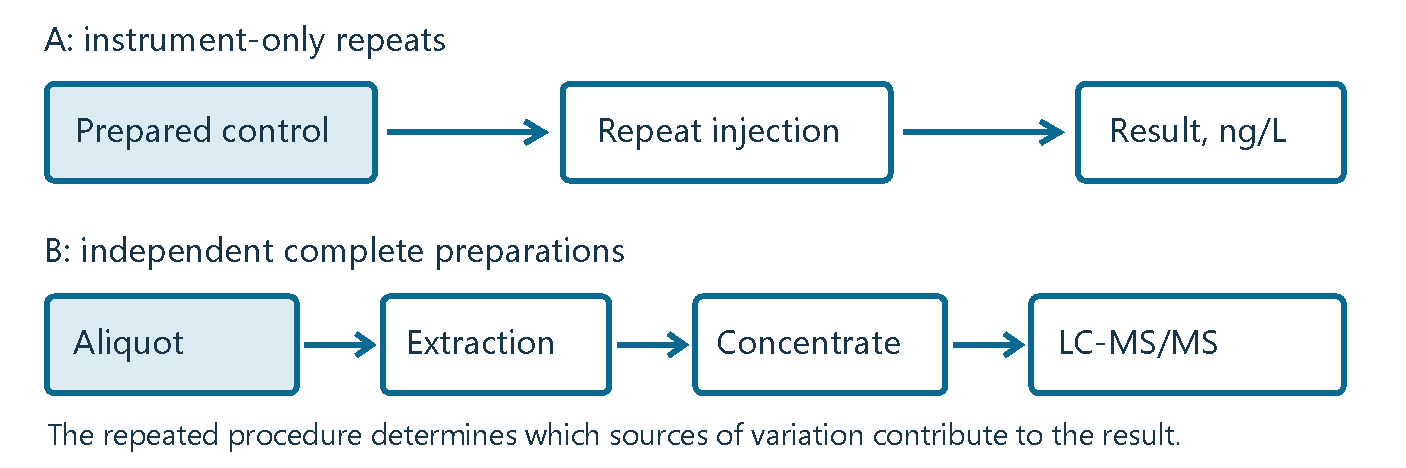
\includegraphics[width=\linewidth,height=.62\textheight,keepaspectratio]{asset-23a67986076f0b4aa74bb94737d4d5addfa99c9b672d90bffe78a6e06e43f6c7.pdf}\end{center}

\medskip

\par\medskip
\Needspace{10cm}
\refstepcounter{figure}\label{material-ff4eaefe23ba8d433aa5254c2c1721ec045f0e136b4ffe4c5cb7226e9c42ef69}
\noindent\textbf{Fig.~\ref*{material-ff4eaefe23ba8d433aa5254c2c1721ec045f0e136b4ffe4c5cb7226e9c42ef69}.} The simulated complete-preparation sample contains 1,000 positive concentrations. Its long right tail includes 100 results above 15 ng/L; this is an observed fraction of this finite simulation.\par\nopagebreak
\begin{center}
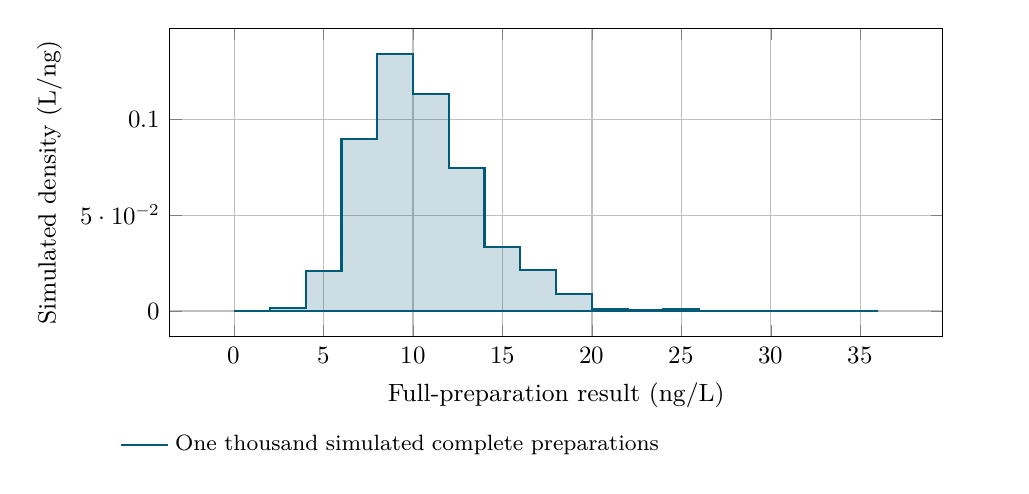
\begin{tikzpicture}
\begin{axis}[width=0.94\linewidth,
height=5.5cm,
scale only axis=false,
grid=major,
tick label style={font=\small},
label style={font=\small},
xlabel={Full-preparation result (ng/L)},
ylabel={Simulated density (L/ng)},
legend style={font=\footnotesize,draw=none,at={(0.5,-0.28)},anchor=north,legend columns=1,text width=0.85\linewidth,align=left},
unbounded coords=jump,
scaled ticks=false]
\addplot[color=pcd1,thick,mark=none,fill=pcd1,fill opacity=0.2] coordinates {(0,0) (0,0) (2,0) (2,0.0015) (4,0.0015) (4,0.021) (6,0.021) (6,0.0895) (8,0.0895) (8,0.134) (10,0.134) (10,0.113) (12,0.113) (12,0.0745) (14,0.0745) (14,0.0335) (16,0.0335) (16,0.0215) (18,0.0215) (18,0.009) (20,0.009) (20,0.001) (22,0.001) (22,0.0005) (24,0.0005) (24,0.001) (26,0.001) (26,0) (28,0) (28,0) (30,0) (30,0) (32,0) (32,0) (34,0) (34,0) (36,0) (36,0)} \closedcycle;
\addlegendentry{One thousand simulated complete preparations}

\end{axis}
\end{tikzpicture}
\end{center}

\medskip

Because a logarithm requires a dimensionless argument, the construction uses a concentration ratio relative to a fixed positive reference concentration. The reference is restored when converting back to concentration. This keeps the model meaningful when concentration units change. The log-scale mean and standard deviation describe the dimensionless log ratio; the original-scale results retain their concentration unit.


On the original scale, equal multiplicative changes occupy unequal additive distances. The resulting distribution can have a long upper tail, with an arithmetic mean above its median. The median describes a typical multiplicative centre, while the arithmetic expectation is relevant for additive totals such as expected load. The analytical question determines which summary is useful.


On a logarithmic horizontal axis, equal relative changes occupy equal distances (\hyperref[material-8abb10753747e027a8b90cfe6b1d4c762c3723af801df66dff826e708cfbe80c]{Fig.~\ref*{material-8abb10753747e027a8b90cfe6b1d4c762c3723af801df66dff826e708cfbe80c}}). Expressing the density itself on the log scale additionally uses the change-of-variable factor, which accounts for how concentration intervals are stretched. Axis scale and density units together determine how the displayed curve is read.


\par\medskip
\Needspace{10cm}
\refstepcounter{figure}\label{material-8abb10753747e027a8b90cfe6b1d4c762c3723af801df66dff826e708cfbe80c}
\noindent\textbf{Fig.~\ref*{material-8abb10753747e027a8b90cfe6b1d4c762c3723af801df66dff826e708cfbe80c}.} The concentrations 8, 10 and 12.5 ng/L have unequal linear gaps. Relative to 10 ng/L their natural log ratios have equal gaps on either side of zero.\par\nopagebreak
\begin{center}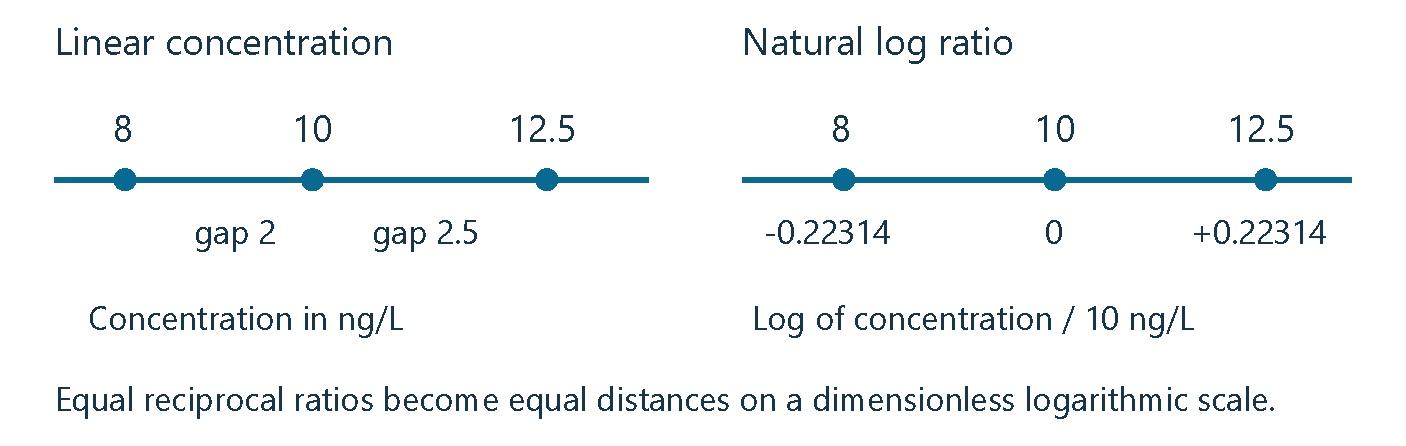
\includegraphics[width=\linewidth,height=.62\textheight,keepaspectratio]{asset-89c42be0226ffb07a0c3ee9b17e0d33b179a20ce89f254acc550eb8b076a9bca.pdf}\end{center}

\medskip

Model-based tail probabilities and quantiles follow from the same positive log-scale construction. The paired questions in \hyperref[material-6b1438bf4a5bab097962b855b890f1e9c111559ba30abad036b2f8bb19813542]{Fig.~\ref*{material-6b1438bf4a5bab097962b855b890f1e9c111559ba30abad036b2f8bb19813542}} distinguish finding a probability from finding a limit. The accompanying formulas retain the reference concentration and distinguish the two scales. Assessing the lognormal model brings together the measurement process, observed variation, possible mixtures and the treatment of nondetects.


\par\medskip
\Needspace{10cm}
\refstepcounter{figure}\label{material-6b1438bf4a5bab097962b855b890f1e9c111559ba30abad036b2f8bb19813542}
\noindent\textbf{Fig.~\ref*{material-6b1438bf4a5bab097962b855b890f1e9c111559ba30abad036b2f8bb19813542}.} The left panel shades the probability above 15 ng/L, about 8.826\%; the right finds the concentration for an upper-tail rate of 5\%, about 16.38 ng/L. Both use median 10 ng/L and dimensionless log SD 0.30.\par\nopagebreak
\begin{center}
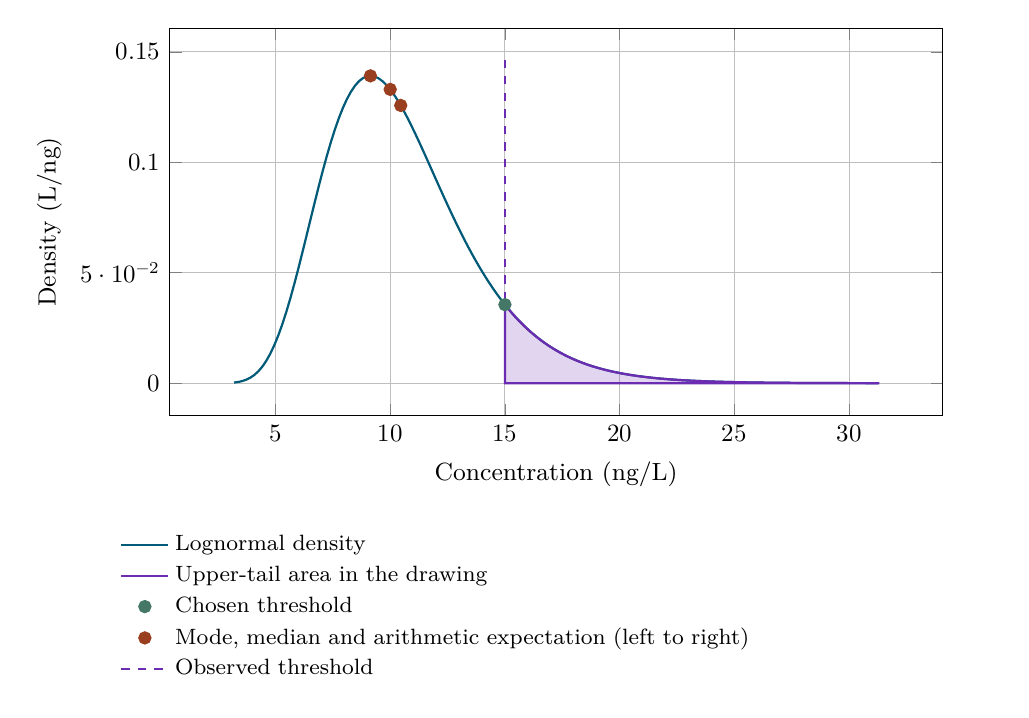
\begin{tikzpicture}
\begin{axis}[width=0.94\linewidth,
height=6.5cm,
scale only axis=false,
grid=major,
tick label style={font=\small},
label style={font=\small},
xlabel={Concentration (ng/L)},
ylabel={Density (L/ng)},
legend style={font=\footnotesize,draw=none,at={(0.5,-0.28)},anchor=north,legend columns=1,text width=0.85\linewidth,align=left},
unbounded coords=jump,
scaled ticks=false]
\addplot[color=pcd1,thick,mark=none] coordinates {(3.1981902181630395,0.00030428347062602933) (3.373624552123655,0.0005584396844081062) (3.549058886084271,0.0009650960446862831) (3.7244932200448866,0.0015819067154850509) (3.8999275540055023,0.0024742409296154067) (4.075361887966118,0.003711897658913977) (4.250796221926734,0.005364931149951211) (4.42623055588735,0.007498998112811781) (4.6016648898479655,0.010170687010424088) (4.777099223808581,0.013423271607800217) (4.952533557769197,0.017283257961947258) (5.127967891729813,0.021757985730677484) (5.303402225690428,0.026834421561310728) (5.478836559651043,0.03247916237763084) (5.65427089361166,0.038639562995001854) (5.8297052275722745,0.04524582375175397) (6.005139561532891,0.05221382291498116) (6.180573895493507,0.059448454712082724) (6.3560082294541225,0.06684723343175653) (6.531442563414738,0.07430394206555355) (6.706876897375354,0.0817121348287935) (6.882311231335969,0.08896834123412838) (7.057745565296585,0.09597486052656141) (7.233179899257202,0.1026420755204125) (7.408614233217817,0.10889025153335842) (7.584048567178433,0.11465081749207431) (7.759482901139048,0.11986715153103293) (7.934917235099665,0.12449491233400112) (8.11035156906028,0.12850197038285247) (8.285785903020896,0.13186800081472455) (8.46122023698151,0.13458380256761115) (8.636654570942127,0.1366504078124289) (8.812088904902742,0.13807804221410416) (8.987523238863359,0.13888499115742392) (9.162957572823974,0.13909642043701037) (9.33839190678459,0.1387431926491421) (9.513826240745205,0.13786071311925918) (9.68926057470582,0.13648783201995962) (9.864694908666436,0.13466582264247576) (10.040129242627053,0.13243744975207342) (10.21556357658767,0.12984613668184028) (10.390997910548284,0.12693523533790196) (10.5664322445089,0.12374739959507401) (10.741866578469516,0.12032405961569197) (10.91730091243013,0.11670499236438928) (11.092735246390747,0.11292798194338234) (11.268169580351364,0.1090285622556564) (11.443603914311979,0.10503983383566363) (11.619038248272595,0.10099234638993798) (11.79447258223321,0.09691403859000133) (11.969906916193827,0.0928302268907235) (12.145341250154441,0.08876363555040392) (12.320775584115056,0.08473446055387954) (12.496209918075673,0.08076046074450509) (12.67164425203629,0.07685707011996873) (12.847078585996904,0.07303752591251943) (13.02251291995752,0.0693130077343523) (13.197947253918136,0.06569278370699522) (13.373381587878752,0.062184360097520666) (13.548815921839367,0.05879363154603688) (13.724250255799982,0.05552502948309544) (13.899684589760598,0.052381666799823895) (14.075118923721215,0.04936547724715858) (14.250553257681831,0.046477348404435306) (14.425987591642446,0.04371724737383798) (14.601421925603061,0.04108433862861671) (14.776856259563678,0.038577093672907715) (14.952290593524292,0.03619339236303486) (15.127724927484909,0.0339306158980968) (15.303159261445524,0.03178573161517934) (15.47859359540614,0.029755369825306657) (15.654027929366757,0.027835893003709762) (15.829462263327372,0.026023457705368035) (16.004896597287985,0.024314069617040673) (16.1803309312486,0.022703632182848366) (16.355765265209218,0.02118798925431853) (16.531199599169835,0.019762962219825753) (16.706633933130448,0.018424382064444224) (16.882068267091064,0.01716811680103492) (17.05750260105168,0.015990094698347078) (17.232936935012297,0.01488632371324328) (17.408371268972914,0.013852907512897743) (17.583805602933527,0.012886058449831485) (17.759239936894144,0.011982107828657901) (17.934674270854757,0.0111375137790023) (18.110108604815377,0.01034886702470306) (18.28554293877599,0.00961289481547546) (18.460977272736606,0.008926463264007525) (18.636411606697223,0.008286578309183909) (18.811845940657836,0.00769038550494927) (18.987280274618456,0.007135168814339119) (19.16271460857907,0.006618348569484995) (19.338148942539686,0.006137478740974073) (19.5135832765003,0.005690243643816845) (19.689017610460915,0.005274454192427934) (19.864451944421532,0.004888043803426259) (20.03988627838215,0.004529064032658567) (20.21532061234276,0.0041956800215939664) (20.390754946303378,0.0038861658180605703) (20.566189280263995,0.003598899627135134) (20.74162361422461,0.003332359039782284) (20.917057948185228,0.003085116279505436) (21.09249228214584,0.002855833500746361) (21.267926616106458,0.0026432581669904196) (21.44336095006707,0.002446218531434607) (21.61879528402769,0.0022636192385954265) (21.794229617988304,0.002094437061315253) (21.96966395194892,0.0019377167842146983) (22.145098285909537,0.001792567241684643) (22.32053261987015,0.0016581575159666743) (22.495966953830766,0.001533713298692354) (22.671401287791383,0.001418513417399128) (22.846835621752,0.0013118865269772725) (23.022269955712613,0.0012132079646949732) (23.19770428967323,0.0011218967663662466) (23.373138623633846,0.0010374128403422517) (23.548572957594462,0.0009592542952949239) (23.72400729155508,0.0008869549172011693) (23.899441625515692,0.0008200817905054205) (24.07487595947631,0.0007582330581205744) (24.25031029343692,0.0007010358147062791) (24.425744627397542,0.0006481441275247465) (24.601178961358155,0.0005992371791055262) (24.77661329531877,0.0005540175259405318) (24.952047629279388,0.000512209467469752) (25.12748196324,0.00047355751969745336) (25.30291629720062,0.0004378249878912497) (25.478350631161234,0.00040479263295543634) (25.65378496512185,0.0003742574262298173) (25.829219299082464,0.00034603138764123287) (26.00465363304308,0.00031994050232261184) (26.180087967003697,0.00029582371101039673) (26.355522300964314,0.0002735319697322558) (26.53095663492493,0.00025292737450081985) (26.706390968885543,0.00023388234693337998) (26.88182530284616,0.0002162788769204086) (27.057259636806776,0.00020000781866587897) (27.232693970767393,0.00018496823661847756) (27.408128304728006,0.0001710667980039824) (27.583562638688623,0.0001582172088545348) (27.75899697264924,0.00014633969060972774) (27.934431306609856,0.00013536049453692094) (28.109865640570472,0.0001252114513836919) (28.285299974531085,0.00011582955383365712) (28.460734308491702,0.00010715656948796639) (28.636168642452315,0.00009913868223857081) (28.81160297641293,0.00009172616003593047) (28.987037310373548,0.00008487304718330219) (29.16247164433416,0.00007853687941223218) (29.33790597829478,0.00007267842010958786) (29.513340312255398,0.00006726141617560281) (29.68877464621601,0.00006225237209517887) (29.864208980176628,0.000057620340901367804) (30.03964331413724,0.000053336730800772964) (30.215077648097857,0.00004937512631582363) (30.390511982058477,0.000045711122878763666) (30.56594631601909,0.00004232217388699159) (30.741380649979707,0.000039187449299375634) (30.91681498394032,0.00003628770491859236) (31.092249317900936,0.00003360516156563033) (31.267683651861557,0.000031123393409633965)};
\addlegendentry{Lognormal density}
\addplot[color=pcd2,thick,mark=none,fill=pcd2,fill opacity=0.2] coordinates {(15,0.03556617908893096) (15.101673022824135,0.03425910588232987) (15.203346045648269,0.032991795597504744) (15.305019068472404,0.03176361304365788) (15.406692091296538,0.030573888570318983) (15.508365114120673,0.02942192248041713) (15.610038136944809,0.028306989167608588) (15.711711159768942,0.027228340986804427) (15.813384182593078,0.026185211867235055) (15.915057205417213,0.025176820677683925) (16.016730228241347,0.02420237435372715) (16.11840325106548,0.023261070796942625) (16.220076273889617,0.022352101556109012) (16.32174929671375,0.02147465430040803) (16.423422319537885,0.020627915094583425) (16.52509534236202,0.019811070485902433) (16.626768365186155,0.019023309412615978) (16.72844138801029,0.018263824943429076) (16.830114410834426,0.017531815857280135) (16.93178743365856,0.016826488072487312) (17.033460456482693,0.016147055934060732) (17.13513347930683,0.015492743367703777) (17.236806502130964,0.014862784908736604) (17.338479524955098,0.014256426613876475) (17.440152547779235,0.013672926863503923) (17.54182557060337,0.013111557061733592) (17.643498593427502,0.012571602241296182) (17.745171616251636,0.012052361579926812) (17.846844639075773,0.011553148834643806) (17.948517661899906,0.01107329269999562) (18.05019068472404,0.010612137096050384) (18.151863707548177,0.010169041391606518) (18.25353673037231,0.00974338056781185) (18.355209753196444,0.00933454532709613) (18.45688277602058,0.008941942152046963) (18.558555798844715,0.008564993318592905) (18.66022882166885,0.00820313686759964) (18.761901844492986,0.007855826538737698) (18.86357486731712,0.007522531670240889) (18.965247890141253,0.007202737067945459) (19.066920912965386,0.00689594284678097) (19.168593935789524,0.00660166424767335) (19.270266958613657,0.006319431432620647) (19.37193998143779,0.0060487892605108895) (19.473613004261928,0.005789297046069977) (19.57528602708606,0.005540528304155237) (19.676959049910195,0.005302070481446296) (19.778632072734332,0.005073524677430795) (19.880305095558466,0.004854505356435536) (19.9819781183826,0.004644640052315741) (20.083651141206737,0.00444356906728499) (20.18532416403087,0.004250945166245534) (20.286997186855004,0.004066433267863462) (20.38867020967914,0.0038897101335252254) (20.490343232503275,0.003720464055210192) (20.592016255327408,0.0035583945432191275) (20.693689278151545,0.0034032120146096074) (20.79536230097568,0.003254637483106318) (20.897035323799813,0.0031124022511769232) (20.99870834662395,0.0029762476048920783) (21.100381369448083,0.0028459245121211117) (21.202054392272217,0.0027211933245527005) (21.303727415096354,0.0026018234839721714) (21.405400437920488,0.0024875932331735752) (21.50707346074462,0.002378289331835207) (21.608746483568755,0.002273706777641833) (21.710419506392892,0.0021736485328945755) (21.812092529217026,0.002077925256811036) (21.91376555204116,0.0019863550436824136) (22.015438574865293,0.001898763167022152) (22.11711159768943,0.0018149818298106063) (22.218784620513564,0.0017348499209132466) (22.320457643337697,0.001658212777725004) (22.422130666161834,0.0015849219550710988) (22.523803688985968,0.0015148350003741156) (22.6254767118101,0.0014478152350788577) (22.72714973463424,0.001383731542309889) (22.828822757458372,0.0013224581607218211) (22.930495780282506,0.0012638744844891327) (23.032168803106643,0.001207864869370528) (23.133841825930777,0.0011543184447723488) (23.23551484875491,0.0011031289317263331) (23.337187871579047,0.0010541944666890418) (23.43886089440318,0.0010074174310632275) (23.540533917227314,0.00096270428633541) (23.64220694005145,0.0009199654147189042) (23.743879962875585,0.0008791149651871845) (23.84555298569972,0.0008400707047789549) (23.947226008523856,0.0008027538750535818) (24.04889903134799,0.0007670890535731721) (24.150572054172123,0.0007330040202861171) (24.25224507699626,0.0007004296286857171) (24.353918099820394,0.0006692996816169396) (24.455591122644528,0.0006395508116041022) (24.55726414546866,0.0006111223655725127) (24.6589371682928,0.0005839562938375823) (24.760610191116932,0.0005579970432357812) (24.862283213941065,0.0005331914542729047) (24.963956236765203,0.0005094886621664974) (25.065629259589336,0.00048684000166081525) (25.16730228241347,0.000465198915494489) (25.268975305237603,0.0004445208664029736) (25.37064832806174,0.0004247632525399138) (25.472321350885874,0.00040588532620377025) (25.573994373710008,0.0003878481157582973) (25.675667396534145,0.0003706143506378991) (25.77734041935828,0.0003541483893312608) (25.879013442182412,0.00033841615023922034) (25.98068646500655,0.00032338504530533043) (26.082359487830683,0.00030902391632018516) (26.184032510654816,0.0002953029738031309) (26.285705533478954,0.0002821937383676147) (26.387378556303087,0.00026966898447903283) (26.48905157912722,0.0002577026865165014) (26.590724601951358,0.00024626996705261195) (26.69239762477549,0.00023534704726775607) (26.794070647599625,0.00022491119941816918) (26.895743670423762,0.00021494070127935053) (26.997416693247896,0.00020541479248899162) (27.09908971607203,0.00019631363271598482) (27.200762738896167,0.00018761826158449624) (27.3024357617203,0.00017931056028442328) (27.404108784544434,0.0001713732148018834) (27.50578180736857,0.00016378968070563163) (27.607454830192705,0.00015654414942752626) (27.709127853016838,0.0001496215159773118) (27.810800875840975,0.0001430073480341065) (27.912473898665105,0.00013668785635903685) (28.014146921489242,0.00013064986647545106) (28.11581994431338,0.0001248807915651191) (28.21749296713751,0.00011936860653069223) (28.319165989961647,0.00011410182317655686) (28.420839012785784,0.00010906946646199849) (28.522512035609914,0.00010426105178232877) (28.62418505843405,0.00009966656323530139) (28.725858081258185,0.0000952764328317923) (28.82753110408232,0.00009108152061127362) (28.929204126906455,0.00008707309562415878) (29.03087714973059,0.00008324281774456443) (29.132550172554723,0.00007958272027846129) (29.23422319537886,0.00007608519333357853) (29.335896218202993,0.00007274296791874608) (29.437569241027127,0.00006954910074165363) (29.539242263851264,0.00006649695967525351) (29.640915286675398,0.00006358020986422006) (29.74258830949953,0.000060792800444045115) (29.84426133232367,0.000058128951846458975) (29.945934355147802,0.000055583143665942356) (30.047607377971936,0.000053150103063121904) (30.14928040079607,0.00005082479368184892) (30.250953423620206,0.00004860240505771017) (30.35262644644434,0.000046478342496644765) (30.454299469268474,0.000044448217403229945) (30.55597249209261,0.000042507838039050276) (30.657645514916744,0.00004065320069238584) (30.759318537740878,0.000038880481241242305) (30.860991560565015,0.00003718602709250595) (30.96266458338915,0.0000355663494807324) (31.064337606213282,0.00003401811611077809) (31.16601062903742,0.00003253814412915498) (31.267683651861553,0.000031123393409633965)} \closedcycle;
\addlegendentry{Upper-tail area in the drawing}
\addplot[color=pcd3,thick,only marks,mark=*] coordinates {(15,0.03556617908893096)};
\addlegendentry{Chosen threshold}
\addplot[color=pcd4,thick,only marks,mark=*] coordinates {(9.139311852712282,0.13910157993180464) (10,0.1329807601338109) (10.46027859908717,0.125707082327716)};
\addlegendentry{Mode, median and arithmetic expectation (left to right)}
\addplot[color=pcd2,dashed,thick] coordinates {(15,0) (15,0.14605665892839487)};
\addlegendentry{Observed threshold}
\end{axis}
\end{tikzpicture}
\end{center}

\begin{center}
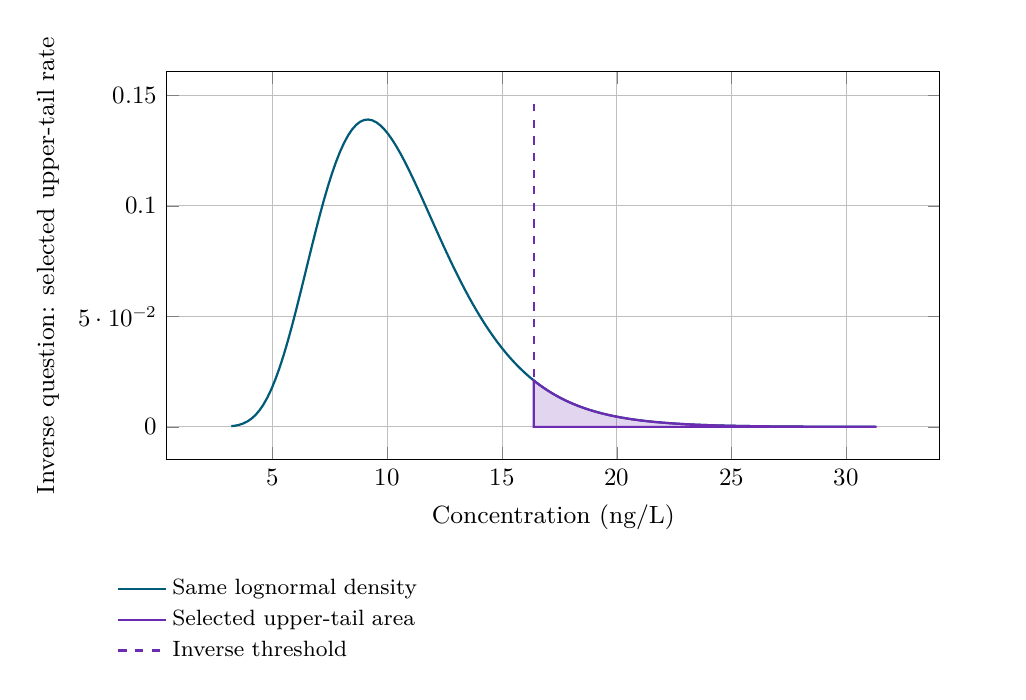
\begin{tikzpicture}
\begin{axis}[width=0.94\linewidth,
height=6.5cm,
scale only axis=false,
grid=major,
tick label style={font=\small},
label style={font=\small},
xlabel={Concentration (ng/L)},
ylabel={Inverse question: selected upper-tail rate},
legend style={font=\footnotesize,draw=none,at={(0.5,-0.28)},anchor=north,legend columns=1,text width=0.85\linewidth,align=left},
unbounded coords=jump,
scaled ticks=false]
\addplot[color=pcd1,thick,mark=none] coordinates {(3.1981902181630395,0.00030428347062602933) (3.373624552123655,0.0005584396844081062) (3.549058886084271,0.0009650960446862831) (3.7244932200448866,0.0015819067154850509) (3.8999275540055023,0.0024742409296154067) (4.075361887966118,0.003711897658913977) (4.250796221926734,0.005364931149951211) (4.42623055588735,0.007498998112811781) (4.6016648898479655,0.010170687010424088) (4.777099223808581,0.013423271607800217) (4.952533557769197,0.017283257961947258) (5.127967891729813,0.021757985730677484) (5.303402225690428,0.026834421561310728) (5.478836559651043,0.03247916237763084) (5.65427089361166,0.038639562995001854) (5.8297052275722745,0.04524582375175397) (6.005139561532891,0.05221382291498116) (6.180573895493507,0.059448454712082724) (6.3560082294541225,0.06684723343175653) (6.531442563414738,0.07430394206555355) (6.706876897375354,0.0817121348287935) (6.882311231335969,0.08896834123412838) (7.057745565296585,0.09597486052656141) (7.233179899257202,0.1026420755204125) (7.408614233217817,0.10889025153335842) (7.584048567178433,0.11465081749207431) (7.759482901139048,0.11986715153103293) (7.934917235099665,0.12449491233400112) (8.11035156906028,0.12850197038285247) (8.285785903020896,0.13186800081472455) (8.46122023698151,0.13458380256761115) (8.636654570942127,0.1366504078124289) (8.812088904902742,0.13807804221410416) (8.987523238863359,0.13888499115742392) (9.162957572823974,0.13909642043701037) (9.33839190678459,0.1387431926491421) (9.513826240745205,0.13786071311925918) (9.68926057470582,0.13648783201995962) (9.864694908666436,0.13466582264247576) (10.040129242627053,0.13243744975207342) (10.21556357658767,0.12984613668184028) (10.390997910548284,0.12693523533790196) (10.5664322445089,0.12374739959507401) (10.741866578469516,0.12032405961569197) (10.91730091243013,0.11670499236438928) (11.092735246390747,0.11292798194338234) (11.268169580351364,0.1090285622556564) (11.443603914311979,0.10503983383566363) (11.619038248272595,0.10099234638993798) (11.79447258223321,0.09691403859000133) (11.969906916193827,0.0928302268907235) (12.145341250154441,0.08876363555040392) (12.320775584115056,0.08473446055387954) (12.496209918075673,0.08076046074450509) (12.67164425203629,0.07685707011996873) (12.847078585996904,0.07303752591251943) (13.02251291995752,0.0693130077343523) (13.197947253918136,0.06569278370699522) (13.373381587878752,0.062184360097520666) (13.548815921839367,0.05879363154603688) (13.724250255799982,0.05552502948309544) (13.899684589760598,0.052381666799823895) (14.075118923721215,0.04936547724715858) (14.250553257681831,0.046477348404435306) (14.425987591642446,0.04371724737383798) (14.601421925603061,0.04108433862861671) (14.776856259563678,0.038577093672907715) (14.952290593524292,0.03619339236303486) (15.127724927484909,0.0339306158980968) (15.303159261445524,0.03178573161517934) (15.47859359540614,0.029755369825306657) (15.654027929366757,0.027835893003709762) (15.829462263327372,0.026023457705368035) (16.004896597287985,0.024314069617040673) (16.1803309312486,0.022703632182848366) (16.355765265209218,0.02118798925431853) (16.531199599169835,0.019762962219825753) (16.706633933130448,0.018424382064444224) (16.882068267091064,0.01716811680103492) (17.05750260105168,0.015990094698347078) (17.232936935012297,0.01488632371324328) (17.408371268972914,0.013852907512897743) (17.583805602933527,0.012886058449831485) (17.759239936894144,0.011982107828657901) (17.934674270854757,0.0111375137790023) (18.110108604815377,0.01034886702470306) (18.28554293877599,0.00961289481547546) (18.460977272736606,0.008926463264007525) (18.636411606697223,0.008286578309183909) (18.811845940657836,0.00769038550494927) (18.987280274618456,0.007135168814339119) (19.16271460857907,0.006618348569484995) (19.338148942539686,0.006137478740974073) (19.5135832765003,0.005690243643816845) (19.689017610460915,0.005274454192427934) (19.864451944421532,0.004888043803426259) (20.03988627838215,0.004529064032658567) (20.21532061234276,0.0041956800215939664) (20.390754946303378,0.0038861658180605703) (20.566189280263995,0.003598899627135134) (20.74162361422461,0.003332359039782284) (20.917057948185228,0.003085116279505436) (21.09249228214584,0.002855833500746361) (21.267926616106458,0.0026432581669904196) (21.44336095006707,0.002446218531434607) (21.61879528402769,0.0022636192385954265) (21.794229617988304,0.002094437061315253) (21.96966395194892,0.0019377167842146983) (22.145098285909537,0.001792567241684643) (22.32053261987015,0.0016581575159666743) (22.495966953830766,0.001533713298692354) (22.671401287791383,0.001418513417399128) (22.846835621752,0.0013118865269772725) (23.022269955712613,0.0012132079646949732) (23.19770428967323,0.0011218967663662466) (23.373138623633846,0.0010374128403422517) (23.548572957594462,0.0009592542952949239) (23.72400729155508,0.0008869549172011693) (23.899441625515692,0.0008200817905054205) (24.07487595947631,0.0007582330581205744) (24.25031029343692,0.0007010358147062791) (24.425744627397542,0.0006481441275247465) (24.601178961358155,0.0005992371791055262) (24.77661329531877,0.0005540175259405318) (24.952047629279388,0.000512209467469752) (25.12748196324,0.00047355751969745336) (25.30291629720062,0.0004378249878912497) (25.478350631161234,0.00040479263295543634) (25.65378496512185,0.0003742574262298173) (25.829219299082464,0.00034603138764123287) (26.00465363304308,0.00031994050232261184) (26.180087967003697,0.00029582371101039673) (26.355522300964314,0.0002735319697322558) (26.53095663492493,0.00025292737450081985) (26.706390968885543,0.00023388234693337998) (26.88182530284616,0.0002162788769204086) (27.057259636806776,0.00020000781866587897) (27.232693970767393,0.00018496823661847756) (27.408128304728006,0.0001710667980039824) (27.583562638688623,0.0001582172088545348) (27.75899697264924,0.00014633969060972774) (27.934431306609856,0.00013536049453692094) (28.109865640570472,0.0001252114513836919) (28.285299974531085,0.00011582955383365712) (28.460734308491702,0.00010715656948796639) (28.636168642452315,0.00009913868223857081) (28.81160297641293,0.00009172616003593047) (28.987037310373548,0.00008487304718330219) (29.16247164433416,0.00007853687941223218) (29.33790597829478,0.00007267842010958786) (29.513340312255398,0.00006726141617560281) (29.68877464621601,0.00006225237209517887) (29.864208980176628,0.000057620340901367804) (30.03964331413724,0.000053336730800772964) (30.215077648097857,0.00004937512631582363) (30.390511982058477,0.000045711122878763666) (30.56594631601909,0.00004232217388699159) (30.741380649979707,0.000039187449299375634) (30.91681498394032,0.00003628770491859236) (31.092249317900936,0.00003360516156563033) (31.267683651861557,0.000031123393409633965)};
\addlegendentry{Same lognormal density}
\addplot[color=pcd2,thick,mark=none,fill=pcd2,fill opacity=0.2] coordinates {(16.379674084724172,0.020988541416616123) (16.472724144518782,0.020228139307996763) (16.56577420431339,0.01949244627146558) (16.658824264108,0.018780841816734124) (16.751874323902605,0.018092708810589404) (16.844924383697215,0.01742743445571075) (16.937974443491825,0.01678441118263167) (17.03102450328643,0.016163037459538655) (17.12407456308104,0.015562718524461571) (17.21712462287565,0.014982867044267309) (17.310174682670258,0.014422903704720201) (17.403224742464868,0.013882257735722854) (17.496274802259475,0.01336036737569882) (17.589324862054085,0.012856680278923775) (17.682374921848695,0.012370653869459979) (17.7754249816433,0.011901755645193886) (17.86847504143791,0.011449463435326076) (17.961525101232517,0.011013265614511854) (18.054575161027127,0.01059266127670316) (18.147625220821737,0.010187160371597167) (18.240675280616344,0.00979628380645496) (18.333725340410954,0.009419563515914595) (18.426775400205564,0.009056542502288345) (18.51982546000017,0.008706774848701885) (18.61287551979478,0.008369825707306579) (18.705925579589387,0.00804527126467267) (18.798975639383997,0.0077326986863520955) (18.892025699178603,0.007431706042485583) (18.985075758973213,0.007141902216217788) (19.078125818767823,0.006862906796578971) (19.17117587856243,0.006594349957389556) (19.26422593835704,0.006335872323647026) (19.35727599815165,0.00608712482676145) (19.450326057946256,0.005847768549916923) (19.543376117740866,0.005617474564751659) (19.636426177535473,0.0053959237604688055) (19.729476237330083,0.005182806666412904) (19.822526297124693,0.004977823269074457) (19.9155763569193,0.004780682824415307) (20.00862641671391,0.004591103666342452) (20.101676476508516,0.004408813012095288) (20.194726536303126,0.004233546765252826) (20.287776596097736,0.004065049317011826) (20.380826655892342,0.003903073346334477) (20.473876715686952,0.0037473796195146734) (20.566926775481562,0.0035977367896659574) (20.65997683527617,0.0034539211965898663) (20.75302689507078,0.0033157166674429315) (20.84607695486539,0.0031829143185817697) (20.939127014659995,0.0030553123589296747) (21.0321770744546,0.0029327158951744023) (21.12522713424921,0.0028149367390751454) (21.21827719404382,0.0027017932171272945) (21.311327253838428,0.0025931099828060355) (21.404377313633038,0.0024887178315841645) (21.497427373427648,0.0023884535188956973) (21.590477433222254,0.002292159581194744) (21.683527493016864,0.0021996841602383794) (21.776577552811474,0.002110880830703543) (21.86962761260608,0.002025608431229942) (21.96267767240069,0.001943730898965062) (22.0557277321953,0.0018651171076721838) (22.148777791989907,0.0017896407094485439) (22.241827851784514,0.0017171799800880464) (22.334877911579124,0.0016476176681114963) (22.427927971373734,0.0015808408474763981) (22.52097803116834,0.00151674077396894) (22.61402809096295,0.001455212745271714) (22.70707815075756,0.0013961559646929256) (22.800128210552167,0.001339473408535361) (22.893178270346777,0.0012850716970769962) (22.986228330141387,0.0012328609691291755) (23.079278389935993,0.0011827547601330173) (23.172328449730603,0.0011346698837500237) (23.26537850952521,0.0010885263168986907) (23.35842856931982,0.0010442470881852927) (23.451478629114426,0.0010017581696737466) (23.544528688909036,0.0009609883719367332) (23.637578748703646,0.0009218692423278524) (23.730628808498253,0.000884334966412569) (23.823678868292863,0.0008483222724939659) (23.916728928087473,0.0008137703391681092) (24.00977898788208,0.000780620705842488) (24.10282904767669,0.0007488171861503884) (24.1958791074713,0.0007183057841933504) (24.288929167265906,0.0006890346135434815) (24.381979227060516,0.000660953818937274) (24.475029286855122,0.0006340155005925578) (24.568079346649732,0.0006081736410803273) (24.66112940644434,0.0005833840346836388) (24.75417946623895,0.0005596042191760468) (24.84722952603356,0.000536793409952797) (24.940279585828165,0.0005149124364485095) (25.033329645622775,0.0004939236807760021) (25.126379705417385,0.0004737910185216548) (25.21942976521199,0.00045447976163372726) (25.3124798250066,0.00043595660334098854) (25.40552988480121,0.0004181895650401163) (25.498579944595818,0.00040114794509140935) (25.591630004390428,0.00038480226946349677) (25.684680064185034,0.0003691242441689598) (25.777730123979644,0.0003540867094339107) (25.87078018377425,0.0003396635955459182) (25.96383024356886,0.0003258298803258076) (26.05688030336347,0.000312561548170243) (26.149930363158077,0.00029983555061317125) (26.242980422952687,0.0002876297683555782) (26.336030482747297,0.0002759229747142294) (26.429080542541904,0.0002646948004413724) (26.522130602336514,0.00025392569986864996) (26.61518066213112,0.0002435969183297495) (26.70823072192573,0.00023369046081754235) (26.80128078172034,0.00022418906183276066) (26.894330841514947,0.00021507615638243359) (26.987380901309557,0.00020633585208756894) (27.080430961104163,0.00019795290236074178) (27.173481020898773,0.00018991268061542435) (27.266531080693383,0.00018220115547007166) (27.35958114048799,0.000174804866911101) (27.4526312002826,0.00016771090338002387) (27.54568126007721,0.00016090687975109328) (27.638731319871816,0.0001543809161668864) (27.731781379666426,0.0001481216177002997) (27.824831439461033,0.0001421180548124743) (27.917881499255643,0.00013635974457713024) (28.01093155905025,0.00013083663264281797) (28.10398161884486,0.0001255390759055021) (28.19703167863947,0.0001204578258648549) (28.290081738434075,0.0001155840126385216) (28.383131798228685,0.0001109091296095092) (28.476181858023295,0.00010642501868270661) (28.569231917817902,0.00010212385612737655) (28.662281977612512,0.0000979981389832621) (28.755332037407122,0.00009404067200875482) (28.84838209720173,0.00009024455515031099) (28.94143215699634,0.00008660317151306141) (29.034482216790945,0.00008311017581327265) (29.127532276585555,0.00007975948329400961) (29.220582336380165,0.00007654525908602937) (29.31363239617477,0.00007346190799658923) (29.40668245596938,0.00007050406470948208) (29.499732515763988,0.00006766658438022687) (29.592782575558598,0.00006494453361093534) (29.685832635353204,0.00006233318178994657) (29.778882695147814,0.00005982799278187948) (29.871932754942424,0.00005742461695428624) (29.964982814737034,0.000055118883527610086) (30.05803287453164,0.00005290679323564665) (30.151082934326247,0.00005078451128420037) (30.244132994120857,0.00004874836059608374) (30.337183053915467,0.00004679481533106531) (30.430233113710077,0.000044920494669805494) (30.523283173504684,0.0000431221568512348) (30.616333233299294,0.00004139669345324119) (30.7093832930939,0.000039741123906917114) (30.80243335288851,0.000038152590234996624) (30.895483412683117,0.00003662835200547606) (30.988533472477727,0.00003516578149175735) (31.081583532272337,0.00003376235903099823) (31.174633592066947,0.00003241566857266868) (31.267683651861553,0.000031123393409633965)} \closedcycle;
\addlegendentry{Selected upper-tail area}
\addplot[color=pcd2,dashed,thick] coordinates {(16.379674084724172,0) (16.379674084724172,0.1460512414588609)};
\addlegendentry{Inverse threshold}
\end{axis}
\end{tikzpicture}
\end{center}

% Full-precision experiment details: {"blockId":"ex:p1-n28-v--block","parameters":[{"key":"reference","label":"Assumed median (ng/L)","value":10},{"key":"logSd","label":"Dimensionless log SD","value":0.3},{"key":"threshold","label":"Chosen threshold (ng/L)","value":15},{"key":"alpha","label":"Prespecified tail / error rate","value":0.05},{"key":"inverse","label":"Inverse mode: 0 threshold, 1 rate","value":0},{"key":"view","label":"Authored inverse / interval view","value":3}],"readouts":[{"label":"Threshold","value":15},{"label":"Standardized distance","value":1.351550360360548},{"label":"Standard-normal density at distance","value":0.16004780590018933},{"label":"Left probability","value":0.9117404003852039},{"label":"Upper probability","value":0.08825959961479607},{"label":"Median","value":10},{"label":"Arithmetic expectation","value":10.46027859908717},{"label":"Mode","value":9.139311852712282},{"label":"Inverse threshold for selected rate","value":16.379674084724172},{"label":"Selected upper-tail rate","value":0.05}],"note":"Probabilities are areas under the density over the full model domain. The displayed examples use explicitly specified model parameters. Left: a probability for the observed threshold. Right: a different threshold for a selected upper-tail rate under the same model.","markers":[[{"x":15,"label":"Observed threshold"}],[{"x":16.379674084724172,"label":"Inverse threshold"}]]}

\medskip

The construction in \hyperref[material-3c159d6152eab0069f9ae1420190e6aa4467fc3254fac2d97aa7e57998ec0bf0]{Eq.~\ref*{material-3c159d6152eab0069f9ae1420190e6aa4467fc3254fac2d97aa7e57998ec0bf0}} uses a dimensionless log ratio; \hyperref[material-07b6a99354255a7bdd43662da1d3b40fdcd6e3827b935fc60c101392bceebbac]{Eq.~\ref*{material-07b6a99354255a7bdd43662da1d3b40fdcd6e3827b935fc60c101392bceebbac}} gives the resulting concentration density and its mean and median. Tail probabilities and concentration limits follow from \hyperref[material-123577ac5b17ce3b2427e4af90077fb60dd4e898213a3c40ae408a61e9be7cae]{Eq.~\ref*{material-123577ac5b17ce3b2427e4af90077fb60dd4e898213a3c40ae408a61e9be7cae}}. The transformation changes symmetry and density units together (\hyperref[material-57efdda451ee1d29f0e43762281f02c40e60826dba67ec0641e5e912056559ef]{Fig.~\ref*{material-57efdda451ee1d29f0e43762281f02c40e60826dba67ec0641e5e912056559ef}}). Optional R examples compare additive and multiplicative models in \hyperref[material-1fbc867cd21f8d74f037b887e497972c934bbbeb61975e919bf02e7ef4f49015]{Listing~\ref*{material-1fbc867cd21f8d74f037b887e497972c934bbbeb61975e919bf02e7ef4f49015}}, reproduce the transformation in \hyperref[material-a3c0a19eed131dd98f7b1917b3ff7b1b39c28f74532c5cc146b4e23f462b13c2]{Listing~\ref*{material-a3c0a19eed131dd98f7b1917b3ff7b1b39c28f74532c5cc146b4e23f462b13c2}} and examine environmental summaries in \hyperref[material-03de4aed76a528b0f00429eb34dc2326983ae42478b69d85e8ab427a2306668f]{Listing~\ref*{material-03de4aed76a528b0f00429eb34dc2326983ae42478b69d85e8ab427a2306668f}}.


\par\medskip
\noindent\begin{minipage}{\linewidth}
\refstepcounter{equation}\label{material-3c159d6152eab0069f9ae1420190e6aa4467fc3254fac2d97aa7e57998ec0bf0}
\noindent\textbf{Eq.~\ref*{material-3c159d6152eab0069f9ae1420190e6aa4467fc3254fac2d97aa7e57998ec0bf0}.} A dimensionless Normal log ratio transformed to positive concentration.\par\nopagebreak
\begin{center}\begin{adjustbox}{max width=\linewidth}$\displaystyle \begin{gathered}\ln(8/10)\approx-0.22314\\\ln(10/10)=0\\\ln(12.5/10)\approx+0.22314\end{gathered}$\end{adjustbox}\end{center}

\par\noindent\textbf{Symbols}

\begin{itemize}\setlength{\itemsep}{1pt}\setlength{\parsep}{0pt}
\item \textbf{ln}: Natural logarithm of a dimensionless ratio.
\item \textbf{/}: Divide a concentration by the reference 10 ng/L; all concentrations use ng/L.
\item \textbf{\ensuremath{-}, +}: Direction below or above zero on the log-ratio scale.
\item \textbf{=, \ensuremath{\approx}}: Equality and approximate equality.
\end{itemize}

The concentrations are 8, 10 and 12.5 ng/L. Reciprocal ratios 0.8 and 1.25 give opposite log values. Equal multiplicative ratios become equal log-scale distances; a Normal log-scale law is a separate model condition.

\end{minipage}\par
\medskip

\par\medskip
\noindent\begin{minipage}{\linewidth}
\refstepcounter{equation}\label{material-07b6a99354255a7bdd43662da1d3b40fdcd6e3827b935fc60c101392bceebbac}
\noindent\textbf{Eq.~\ref*{material-07b6a99354255a7bdd43662da1d3b40fdcd6e3827b935fc60c101392bceebbac}.} Lognormal density, cumulative probability, expectation and median on the concentration scale.\par\nopagebreak
\begin{center}\begin{adjustbox}{max width=\linewidth}$\displaystyle \begin{gathered}Y=\ln(X/x_{\mathrm{ref}})\sim\mathcal N(\mu_L,\sigma_L^2)\\X=x_{\mathrm{ref}}e^Y\end{gathered}$\end{adjustbox}\end{center}

\par\noindent\textbf{Symbols}

\begin{itemize}\setlength{\itemsep}{1pt}\setlength{\parsep}{0pt}
\item \textbf{X}: Positive random concentration (ng/L).
\item \textbf{\(x_{ref}\)}: Fixed positive reference concentration, 10 ng/L; subscript ref means reference.
\item \textbf{\(Y\)}: Natural log ratio \(\ln(X / x_{ref})\), dimensionless.
\item \textbf{\(μ_L\)}: Mean of the log ratio, dimensionless; subscript L identifies the log scale.
\item \textbf{\(σ_L\)}: Positive SD of the log ratio, dimensionless.
\item \textbf{\(N, ∼\)}: Normal distribution; follows that distribution. Its second parameter is variance \(σ_L^2\).
\item \textbf{ln, e}: Natural logarithm and the base of the natural exponential.
\item \textbf{/, \ensuremath{{}^2}, =}: Division, squaring and equality defining the transforms.
\end{itemize}

Here \(μ_L = 0\) and \(σ_L = 0.30\), giving median 10 ng/L. Multiplying the exponentiated ratio by the reference restores concentration units.

\end{minipage}\par
\medskip

\par\medskip
\noindent\begin{minipage}{\linewidth}
\refstepcounter{equation}\label{material-123577ac5b17ce3b2427e4af90077fb60dd4e898213a3c40ae408a61e9be7cae}
\noindent\textbf{Eq.~\ref*{material-123577ac5b17ce3b2427e4af90077fb60dd4e898213a3c40ae408a61e9be7cae}.} Lognormal concentration quantiles and upper-tail probabilities.\par\nopagebreak
\begin{center}\begin{adjustbox}{max width=\linewidth}$\displaystyle \begin{gathered}z_{0.95}=\Phi^{-1}(0.95)\approx1.64485\\x_{0.95}=x_{\mathrm{ref}}\exp(\mu_L+\sigma_L z_{0.95})\\\approx16.38\;\mathrm{ng/L}\end{gathered}$\end{adjustbox}\end{center}

\par\noindent\textbf{Symbols}

\begin{itemize}\setlength{\itemsep}{1pt}\setlength{\parsep}{0pt}
\item \textbf{z\ensuremath{{}_0}.\ensuremath{{}_9}\ensuremath{{}_5}}: Standard-normal 95th percentile (dimensionless).
\item \textbf{x\ensuremath{{}_0}.\ensuremath{{}_9}\ensuremath{{}_5}}: Corresponding concentration percentile (ng/L); subscript 0.95 is the cumulative probability.
\item \textbf{\(x_{ref}\)}: Reference concentration, 10 ng/L.
\item \textbf{\(μ_L\)}: Log-ratio mean, 0; subscript L denotes the log scale.
\item \textbf{\(σ_L\)}: Log-ratio SD, 0.30 (dimensionless).
\item \textbf{\ensuremath{\Phi}\ensuremath{{}^-}\ensuremath{{}^1}}: Inverse standard-normal CDF, mapping cumulative probability to a z value.
\item \textbf{exp}: Natural exponential, applied to the dimensionless log-scale value.
\item \textbf{+, =, \ensuremath{\approx}}: Addition, equality and approximate equality; adjacent factors multiply.
\end{itemize}

The unrounded quantile is 16.3796740847 ng/L. This is a per-result model threshold; rounding, resolution and estimated parameters matter when constructing a real rule.

\end{minipage}\par
\medskip

\par\medskip
\Needspace{10cm}
\refstepcounter{figure}\label{material-57efdda451ee1d29f0e43762281f02c40e60826dba67ec0641e5e912056559ef}
\noindent\textbf{Fig.~\ref*{material-57efdda451ee1d29f0e43762281f02c40e60826dba67ec0641e5e912056559ef}.} The left panel shows the Normal density of the dimensionless log ratio with mean 0 and SD 0.30. The right panel shows its exponential concentration transform relative to 10 ng/L, giving a lognormal distribution with median 10 ng/L.\par\nopagebreak
\begin{center}
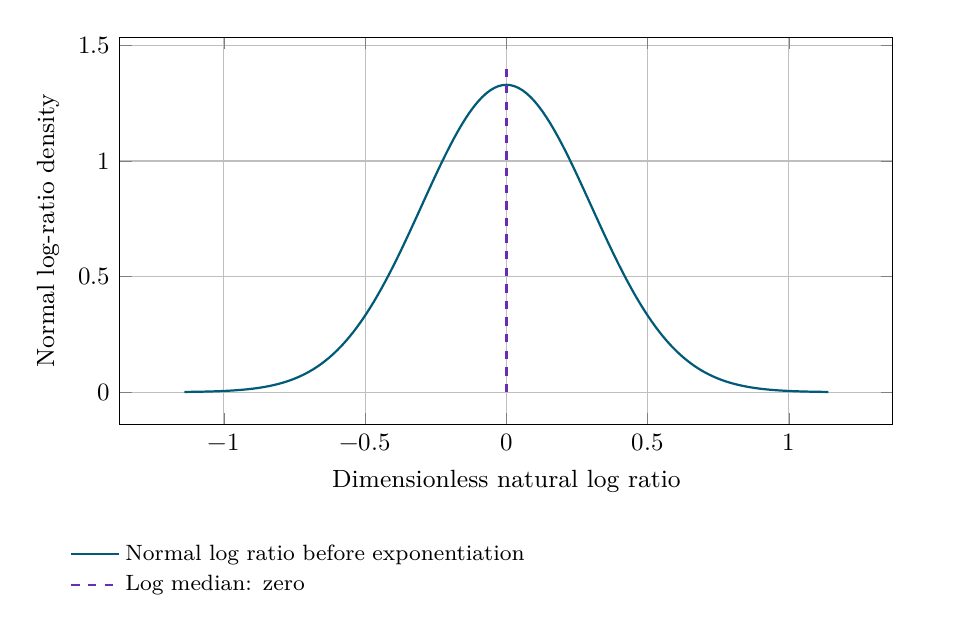
\begin{tikzpicture}
\begin{axis}[width=0.94\linewidth,
height=6.5cm,
scale only axis=false,
grid=major,
tick label style={font=\small},
label style={font=\small},
xlabel={Dimensionless natural log ratio},
ylabel={Normal log-ratio density},
legend style={font=\footnotesize,draw=none,at={(0.5,-0.28)},anchor=north,legend columns=1,text width=0.85\linewidth,align=left},
unbounded coords=jump,
scaled ticks=false]
\addplot[color=pcd1,thick,mark=none] coordinates {(-1.14,0.0009731564193048676) (-1.1257499999999998,0.001164348176287353) (-1.1115,0.0013899628916108555) (-1.0972499999999998,0.001655555207041624) (-1.083,0.0019674524830759522) (-1.0687499999999999,0.0023328400364898134) (-1.0545,0.0027598519862021796) (-1.04025,0.0032576674237967413) (-1.0259999999999998,0.003836611480594952) (-1.01175,0.004508260700335763) (-0.9974999999999999,0.005285551945498195) (-0.98325,0.006182893866791166) (-0.9689999999999999,0.00721627975057022) (-0.95475,0.008403400329777759) (-0.9404999999999999,0.009763754902976002) (-0.9262499999999999,0.01131875885640258) (-0.9119999999999999,0.013091845429749263) (-0.8977499999999999,0.015108559312338085) (-0.8835,0.01739663940813265) (-0.86925,0.01998608787191593) (-0.855,0.02290922230204657) (-0.8407499999999999,0.0262007077851725) (-0.8264999999999999,0.029897565333361274) (-0.8122499999999999,0.034039153142930004) (-0.7979999999999999,0.03866711704567524) (-0.78375,0.043825306526098666) (-0.7695,0.049559652751268786) (-0.75525,0.05591800521136518) (-0.7409999999999999,0.06294992380618729) (-0.72675,0.07070642354239376) (-0.7124999999999999,0.07923966943304603) (-0.6982499999999999,0.08860261971855268) (-0.6839999999999999,0.09884861615780427) (-0.66975,0.11003092086930384) (-0.6555,0.12220220003111756) (-0.6412499999999999,0.13541395566941125) (-0.6269999999999999,0.14971590776922367) (-0.6127499999999999,0.1651553300159874) (-0.5985,0.18177634360710793) (-0.5842499999999999,0.19961917474167687) (-0.57,0.21871938258225532) (-0.55575,0.2391070656622108) (-0.5415,0.26080605585958383) (-0.52725,0.2838331101464061) (-0.5129999999999999,0.3081971113219357) (-0.4987499999999999,0.33389828981993075) (-0.48449999999999993,0.3609274794143929) (-0.47024999999999995,0.3892654202064613) (-0.45599999999999996,0.41888212263029384) (-0.44175,0.4497363063431443) (-0.4275,0.4817749277431096) (-0.41325,0.5149328094698834) (-0.399,0.5491323845769228) (-0.3847499999999999,0.5842835671108646) (-0.37049999999999994,0.6202837595951243) (-0.35624999999999996,0.6570180063952911) (-0.34199999999999997,0.694359300157028) (-0.32775,0.7321690464726148) (-0.3135,0.7702976896769377) (-0.29925,0.8085855002313018) (-0.28500000000000003,0.8468635215639633) (-0.27075000000000005,0.8849546715453612) (-0.25649999999999995,0.9226749910342091) (-0.24224999999999997,0.9598350291921525) (-0.22799999999999998,0.9962413525865093) (-0.21375,1.0316981625409136) (-0.1995,1.066009002810549) (-0.18524999999999991,1.0989785375086318) (-0.17099999999999993,1.1304143773473074) (-0.15674999999999994,1.1601289307280813) (-0.14249999999999996,1.1879412550672777) (-0.12824999999999998,1.2136788830065874) (-0.11399999999999988,1.237179597864887) (-0.09975,1.258293132853382) (-0.08549999999999991,1.2768827692098128) (-0.07125000000000004,1.292826809506695) (-0.05700000000000016,1.3060199039404037) (-0.042750000000000066,1.3163742093888864) (-0.02849999999999997,1.3238203634023324) (-0.014250000000000096,1.3283082580202032) (0,1.329807601338109) (0.014249999999999874,1.3283082580202035) (0.02849999999999997,1.3238203634023324) (0.042750000000000066,1.3163742093888864) (0.05699999999999994,1.306019903940404) (0.07125000000000004,1.292826809506695) (0.08549999999999991,1.2768827692098128) (0.09975,1.258293132853382) (0.1140000000000001,1.2371795978648867) (0.12824999999999998,1.2136788830065874) (0.14250000000000007,1.1879412550672774) (0.15674999999999994,1.1601289307280813) (0.17100000000000004,1.1304143773473072) (0.18525000000000014,1.0989785375086312) (0.1995,1.066009002810549) (0.2137500000000001,1.0316981625409134) (0.22799999999999998,0.9962413525865093) (0.24224999999999985,0.9598350291921528) (0.25649999999999995,0.9226749910342091) (0.2707499999999998,0.8849546715453618) (0.2849999999999999,0.8468635215639636) (0.29925,0.8085855002313018) (0.3134999999999999,0.770297689676938) (0.32775,0.7321690464726148) (0.34199999999999986,0.6943593001570282) (0.35624999999999996,0.6570180063952911) (0.37050000000000005,0.6202837595951238) (0.3847499999999999,0.5842835671108646) (0.399,0.5491323845769228) (0.4132499999999999,0.5149328094698836) (0.4275,0.4817749277431096) (0.4417500000000001,0.44973630634314404) (0.45599999999999996,0.41888212263029384) (0.47025000000000006,0.389265420206461) (0.48449999999999993,0.3609274794143929) (0.49875,0.33389828981993064) (0.5129999999999999,0.3081971113219357) (0.52725,0.2838331101464061) (0.5414999999999999,0.26080605585958394) (0.55575,0.2391070656622108) (0.5699999999999998,0.2187193825822555) (0.5842500000000002,0.19961917474167656) (0.5984999999999998,0.18177634360710818) (0.6127500000000001,0.16515533001598717) (0.627,0.14971590776922356) (0.6412500000000001,0.13541395566941092) (0.6555,0.12220220003111756) (0.6697500000000001,0.11003092086930374) (0.6839999999999999,0.09884861615780427) (0.6982499999999998,0.08860261971855268) (0.7124999999999999,0.07923966943304603) (0.7267499999999998,0.0707064235423939) (0.7409999999999999,0.06294992380618729) (0.7552499999999998,0.05591800521136531) (0.7695000000000001,0.04955965275126874) (0.7837499999999997,0.04382530652609872) (0.798,0.03866711704567521) (0.8122499999999999,0.034039153142930004) (0.8265,0.02989756533336125) (0.8407499999999999,0.0262007077851725) (0.855,0.02290922230204657) (0.8692499999999999,0.019986087871915966) (0.8835,0.01739663940813265) (0.89775,0.015108559312338073) (0.9120000000000001,0.013091845429749241) (0.9262499999999998,0.01131875885640259) (0.9404999999999999,0.009763754902976002) (0.95475,0.008403400329777759) (0.9690000000000001,0.007216279750570195) (0.9832499999999997,0.006182893866791177) (0.9974999999999998,0.005285551945498195) (1.01175,0.004508260700335763) (1.0259999999999996,0.003836611480594965) (1.0402500000000001,0.003257667423796732) (1.0544999999999998,0.0027598519862021874) (1.0687499999999999,0.0023328400364898134) (1.083,0.0019674524830759522) (1.09725,0.0016555552070416212) (1.1114999999999997,0.0013899628916108605) (1.1257499999999998,0.001164348176287353) (1.14,0.0009731564193048676)};
\addlegendentry{Normal log ratio before exponentiation}
\addplot[color=pcd2,dashed,thick] coordinates {(0,0) (0,1.3962979814050145)};
\addlegendentry{Log median: zero}
\end{axis}
\end{tikzpicture}
\end{center}

\begin{center}
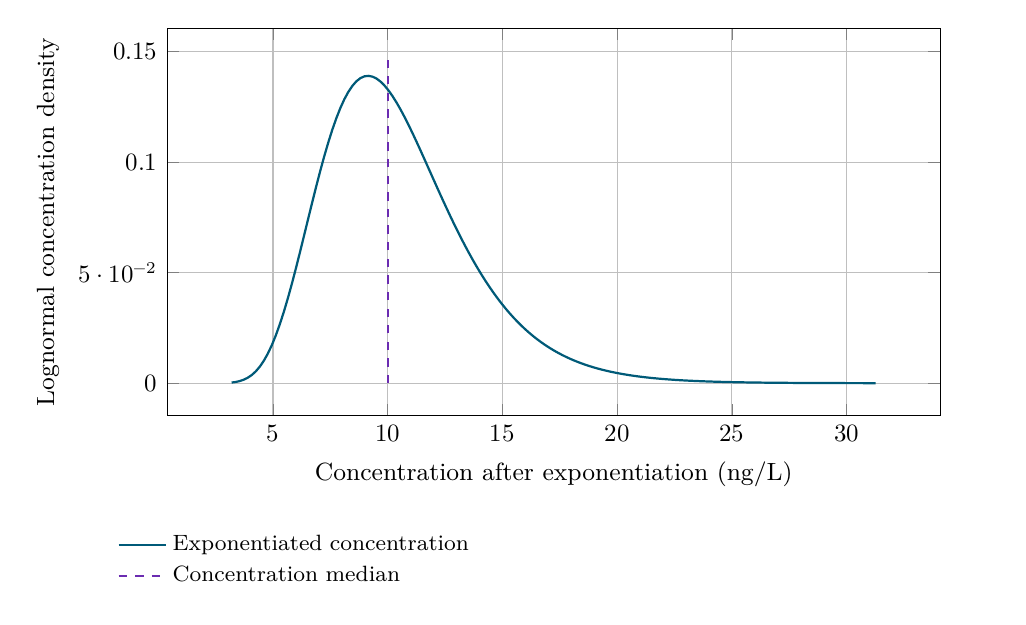
\begin{tikzpicture}
\begin{axis}[width=0.94\linewidth,
height=6.5cm,
scale only axis=false,
grid=major,
tick label style={font=\small},
label style={font=\small},
xlabel={Concentration after exponentiation (ng/L)},
ylabel={Lognormal concentration density},
legend style={font=\footnotesize,draw=none,at={(0.5,-0.28)},anchor=north,legend columns=1,text width=0.85\linewidth,align=left},
unbounded coords=jump,
scaled ticks=false]
\addplot[color=pcd1,thick,mark=none] coordinates {(3.1981902181630395,0.00030428347062602933) (3.373624552123655,0.0005584396844081062) (3.549058886084271,0.0009650960446862831) (3.7244932200448866,0.0015819067154850509) (3.8999275540055023,0.0024742409296154067) (4.075361887966118,0.003711897658913977) (4.250796221926734,0.005364931149951211) (4.42623055588735,0.007498998112811781) (4.6016648898479655,0.010170687010424088) (4.777099223808581,0.013423271607800217) (4.952533557769197,0.017283257961947258) (5.127967891729813,0.021757985730677484) (5.303402225690428,0.026834421561310728) (5.478836559651043,0.03247916237763084) (5.65427089361166,0.038639562995001854) (5.8297052275722745,0.04524582375175397) (6.005139561532891,0.05221382291498116) (6.180573895493507,0.059448454712082724) (6.3560082294541225,0.06684723343175653) (6.531442563414738,0.07430394206555355) (6.706876897375354,0.0817121348287935) (6.882311231335969,0.08896834123412838) (7.057745565296585,0.09597486052656141) (7.233179899257202,0.1026420755204125) (7.408614233217817,0.10889025153335842) (7.584048567178433,0.11465081749207431) (7.759482901139048,0.11986715153103293) (7.934917235099665,0.12449491233400112) (8.11035156906028,0.12850197038285247) (8.285785903020896,0.13186800081472455) (8.46122023698151,0.13458380256761115) (8.636654570942127,0.1366504078124289) (8.812088904902742,0.13807804221410416) (8.987523238863359,0.13888499115742392) (9.162957572823974,0.13909642043701037) (9.33839190678459,0.1387431926491421) (9.513826240745205,0.13786071311925918) (9.68926057470582,0.13648783201995962) (9.864694908666436,0.13466582264247576) (10.040129242627053,0.13243744975207342) (10.21556357658767,0.12984613668184028) (10.390997910548284,0.12693523533790196) (10.5664322445089,0.12374739959507401) (10.741866578469516,0.12032405961569197) (10.91730091243013,0.11670499236438928) (11.092735246390747,0.11292798194338234) (11.268169580351364,0.1090285622556564) (11.443603914311979,0.10503983383566363) (11.619038248272595,0.10099234638993798) (11.79447258223321,0.09691403859000133) (11.969906916193827,0.0928302268907235) (12.145341250154441,0.08876363555040392) (12.320775584115056,0.08473446055387954) (12.496209918075673,0.08076046074450509) (12.67164425203629,0.07685707011996873) (12.847078585996904,0.07303752591251943) (13.02251291995752,0.0693130077343523) (13.197947253918136,0.06569278370699522) (13.373381587878752,0.062184360097520666) (13.548815921839367,0.05879363154603688) (13.724250255799982,0.05552502948309544) (13.899684589760598,0.052381666799823895) (14.075118923721215,0.04936547724715858) (14.250553257681831,0.046477348404435306) (14.425987591642446,0.04371724737383798) (14.601421925603061,0.04108433862861671) (14.776856259563678,0.038577093672907715) (14.952290593524292,0.03619339236303486) (15.127724927484909,0.0339306158980968) (15.303159261445524,0.03178573161517934) (15.47859359540614,0.029755369825306657) (15.654027929366757,0.027835893003709762) (15.829462263327372,0.026023457705368035) (16.004896597287985,0.024314069617040673) (16.1803309312486,0.022703632182848366) (16.355765265209218,0.02118798925431853) (16.531199599169835,0.019762962219825753) (16.706633933130448,0.018424382064444224) (16.882068267091064,0.01716811680103492) (17.05750260105168,0.015990094698347078) (17.232936935012297,0.01488632371324328) (17.408371268972914,0.013852907512897743) (17.583805602933527,0.012886058449831485) (17.759239936894144,0.011982107828657901) (17.934674270854757,0.0111375137790023) (18.110108604815377,0.01034886702470306) (18.28554293877599,0.00961289481547546) (18.460977272736606,0.008926463264007525) (18.636411606697223,0.008286578309183909) (18.811845940657836,0.00769038550494927) (18.987280274618456,0.007135168814339119) (19.16271460857907,0.006618348569484995) (19.338148942539686,0.006137478740974073) (19.5135832765003,0.005690243643816845) (19.689017610460915,0.005274454192427934) (19.864451944421532,0.004888043803426259) (20.03988627838215,0.004529064032658567) (20.21532061234276,0.0041956800215939664) (20.390754946303378,0.0038861658180605703) (20.566189280263995,0.003598899627135134) (20.74162361422461,0.003332359039782284) (20.917057948185228,0.003085116279505436) (21.09249228214584,0.002855833500746361) (21.267926616106458,0.0026432581669904196) (21.44336095006707,0.002446218531434607) (21.61879528402769,0.0022636192385954265) (21.794229617988304,0.002094437061315253) (21.96966395194892,0.0019377167842146983) (22.145098285909537,0.001792567241684643) (22.32053261987015,0.0016581575159666743) (22.495966953830766,0.001533713298692354) (22.671401287791383,0.001418513417399128) (22.846835621752,0.0013118865269772725) (23.022269955712613,0.0012132079646949732) (23.19770428967323,0.0011218967663662466) (23.373138623633846,0.0010374128403422517) (23.548572957594462,0.0009592542952949239) (23.72400729155508,0.0008869549172011693) (23.899441625515692,0.0008200817905054205) (24.07487595947631,0.0007582330581205744) (24.25031029343692,0.0007010358147062791) (24.425744627397542,0.0006481441275247465) (24.601178961358155,0.0005992371791055262) (24.77661329531877,0.0005540175259405318) (24.952047629279388,0.000512209467469752) (25.12748196324,0.00047355751969745336) (25.30291629720062,0.0004378249878912497) (25.478350631161234,0.00040479263295543634) (25.65378496512185,0.0003742574262298173) (25.829219299082464,0.00034603138764123287) (26.00465363304308,0.00031994050232261184) (26.180087967003697,0.00029582371101039673) (26.355522300964314,0.0002735319697322558) (26.53095663492493,0.00025292737450081985) (26.706390968885543,0.00023388234693337998) (26.88182530284616,0.0002162788769204086) (27.057259636806776,0.00020000781866587897) (27.232693970767393,0.00018496823661847756) (27.408128304728006,0.0001710667980039824) (27.583562638688623,0.0001582172088545348) (27.75899697264924,0.00014633969060972774) (27.934431306609856,0.00013536049453692094) (28.109865640570472,0.0001252114513836919) (28.285299974531085,0.00011582955383365712) (28.460734308491702,0.00010715656948796639) (28.636168642452315,0.00009913868223857081) (28.81160297641293,0.00009172616003593047) (28.987037310373548,0.00008487304718330219) (29.16247164433416,0.00007853687941223218) (29.33790597829478,0.00007267842010958786) (29.513340312255398,0.00006726141617560281) (29.68877464621601,0.00006225237209517887) (29.864208980176628,0.000057620340901367804) (30.03964331413724,0.000053336730800772964) (30.215077648097857,0.00004937512631582363) (30.390511982058477,0.000045711122878763666) (30.56594631601909,0.00004232217388699159) (30.741380649979707,0.000039187449299375634) (30.91681498394032,0.00003628770491859236) (31.092249317900936,0.00003360516156563033) (31.267683651861557,0.000031123393409633965)};
\addlegendentry{Exponentiated concentration}
\addplot[color=pcd2,dashed,thick] coordinates {(10,0) (10,0.1460512414588609)};
\addlegendentry{Concentration median}
\end{axis}
\end{tikzpicture}
\end{center}

% Full-precision experiment details: {"blockId":"ex:rv-log-v--block","parameters":[{"key":"reference","label":"Assumed median (ng/L)","value":10},{"key":"logSd","label":"Dimensionless log SD","value":0.3},{"key":"threshold","label":"Chosen threshold (ng/L)","value":15},{"key":"alpha","label":"Prespecified tail / error rate","value":0.05},{"key":"inverse","label":"Inverse mode: 0 threshold, 1 rate","value":0},{"key":"view","label":"Authored comparison / transformation view","value":1}],"readouts":[{"label":"Median","value":10},{"label":"Dimensionless log SD","value":0.3}],"note":"Probabilities are areas under the density over the full model domain. The displayed examples use explicitly specified model parameters. Exponentiation maps dimensionless Normal log ratios to positive concentrations. The change-of-variable factor relates the density heights on the two scales.","markers":[[{"x":0,"label":"Log median: zero"}],[{"x":10,"label":"Concentration median"}]]}

\medskip

\par\medskip
\Needspace{8\baselineskip}
\refstepcounter{listing}\label{material-1fbc867cd21f8d74f037b887e497972c934bbbeb61975e919bf02e7ef4f49015}
\noindent\textbf{Listing~\ref*{material-1fbc867cd21f8d74f037b887e497972c934bbbeb61975e919bf02e7ef4f49015}.} R comparison of additive and multiplicative measurement models.\par\nopagebreak
\begin{Verbatim}[fontsize=\footnotesize,breaklines=true,breakanywhere=true]
# Separate fictional series, not paired validation measurements.
# Relative factors are NOT literal unbounded extraction recoveries.
M <- 1000; steps <- 3; factor_model <- 'normal'
x0 <- 10; sd_instrument <- 0.10; sigma_L <- 0.30; state <- 20261103
stopifnot(M>=10,M<=10000,steps>=1,steps<=200,
          factor_model %in% c('normal','binary'))
A <- numeric(M); B <- numeric(M); log_total <- numeric(M)
for(j in seq_len(M)) {
  state <- (16807*state) %% 2147483647
  A[j] <- x0+sd_instrument*qnorm(state/2147483647)
  contributions <- numeric(steps)
  for(i in seq_len(steps)) {
    state <- (16807*state) %% 2147483647
    u <- state/2147483647
    contributions[i] <- sigma_L/sqrt(steps) *
      if(factor_model=='normal') qnorm(u) else if(u<0.5) -1 else 1
  }
  log_total[j] <- sum(contributions)
  B[j] <- x0*prod(exp(contributions))
}
cat('Instrument mean and SD (ng/L):',mean(A),sd(A),'\n')
cat('Preparation mean (ng/L):',mean(B),'log SD:',sd(log_total),'\n')
cat('Preparation count above 15 ng/L:',sum(B>15),'of',M,'\n')
edges_B <- seq(0,max(36,ceiling(max(B)/2)*2),by=2)
hB <- hist(B,breaks=edges_B,right=FALSE,plot=FALSE)
cat('Preparation bin counts:',hB$counts,'\n')
cat('Normal log factors: exact lognormal. Binary log factors: finite discrete model.\n')
old <- par(mfrow=c(1,2),mar=c(5,4,3,1))
hist(A,breaks=seq(floor(min(A)/.05)*.05,ceiling(max(A)/.05)*.05,by=.05),
     right=FALSE,probability=TRUE,col='#8ecae6',main='A: instrument only',
     xlab='Result (ng/L)',ylab='Density (L/ng)')
plot(hB,freq=FALSE,col='#8ecae6',main='B: complete preparation',
     xlab='Result (ng/L)',ylab='Density (L/ng)')
par(old)
cat('Panel ranges differ; the concentration units are the same.\n')

\end{Verbatim}

\medskip

\par\medskip
\Needspace{8\baselineskip}
\refstepcounter{listing}\label{material-a3c0a19eed131dd98f7b1917b3ff7b1b39c28f74532c5cc146b4e23f462b13c2}
\noindent\textbf{Listing~\ref*{material-a3c0a19eed131dd98f7b1917b3ff7b1b39c28f74532c5cc146b4e23f462b13c2}.} R transformation between dimensionless log ratios and concentration.\par\nopagebreak
\begin{Verbatim}[fontsize=\footnotesize,breaklines=true,breakanywhere=true]
# Fixed median 10 ng/L; log SD changes, not the reference units.
M <- 10000; x_ref <- 10; mu_L <- 0; sigma_L <- 0.30; state <- 20261103
stopifnot(M>=100,M<=10000,x_ref>0,sigma_L>0,sigma_L<=1)
Y <- numeric(M)
for(i in seq_len(M)) {
  state <- (16807*state) %% 2147483647
  Y[i] <- mu_L+sigma_L*qnorm(state/2147483647)
}
X <- x_ref*exp(Y)
model_mode <- x_ref*exp(mu_L-sigma_L^2)
model_median <- x_ref*exp(mu_L)
model_mean <- x_ref*exp(mu_L+sigma_L^2/2)
cat('Population mode, median, mean (ng/L):',model_mode,model_median,model_mean,'\n')
cat('Sample geometric mean (ng/L):',x_ref*exp(mean(log(X/x_ref))),'\n')
cat('Upper probability above 15 ng/L:',pnorm((log(15/x_ref)-mu_L)/sigma_L,lower.tail=FALSE),'\n')
q95 <- x_ref*exp(mu_L+sigma_L*qnorm(.95))
cat('Population 95th percentile (ng/L):',format(q95,digits=12),'\n')
old <- par(mfrow=c(1,3),mar=c(5,4,3,1))
hist(Y,probability=TRUE,col='#8ecae6',main='Normal log ratios',
     xlab='Y: natural log ratio',ylab='Density per log-ratio unit')
curve(dnorm(x,mu_L,sigma_L),add=TRUE,col='#a63d21',lwd=2)
hist(X,probability=TRUE,col='#8ecae6',main='Exponentiated results',
     xlab='Concentration (ng/L)',ylab='Density (L/ng)')
curve(dlnorm(x/x_ref,meanlog=mu_L,sdlog=sigma_L)/x_ref,
      add=TRUE,col='#a63d21',lwd=2)
grid <- seq(.01,35,length.out=1000)
spreads <- c(.15,.30,.60); colors <- c('#176b90','#a63d21','#5c469c')
densities <- sapply(spreads,function(s) dlnorm(grid/x_ref,mu_L,s)/x_ref)
matplot(grid,densities,type='l',lty=1,col=colors,lwd=2,
        xlab='Concentration (ng/L)',ylab='Density (L/ng)',main='Same median, different log SD')
legend('topright',legend=spreads,col=colors,lty=1,bty='n',title='Log SD')
par(old)
cat('The comparison-density window ends at 35; tails and moments are not truncated.\n')

\end{Verbatim}

\medskip

\par\medskip
\Needspace{8\baselineskip}
\refstepcounter{listing}\label{material-03de4aed76a528b0f00429eb34dc2326983ae42478b69d85e8ab427a2306668f}
\noindent\textbf{Listing~\ref*{material-03de4aed76a528b0f00429eb34dc2326983ae42478b69d85e8ab427a2306668f}.} R illustration of lognormal environmental concentration summaries.\par\nopagebreak
\begin{Verbatim}[fontsize=\footnotesize,breaklines=true,breakanywhere=true]
# New population: between-site concentrations, NOT technical repeats.
M <- 100; mode <- 'candidate'; x_ref <- 10; sigma_site <- 0.60
loq <- 5; state <- 20261103
stopifnot(mode %in% c('candidate','mixture','censored'))
log_ratio <- numeric(M)
for(i in seq_len(M)) {
  state <- (16807*state) %% 2147483647
  log_ratio[i] <- sigma_site*qnorm(state/2147483647)
}
if(mode=='mixture') {
  for(i in seq_len(M)) {
    state <- (16807*state) %% 2147483647
    if(state/2147483647<.30) log_ratio[i] <- log_ratio[i]+1.2
  }
}
latent <- x_ref*exp(log_ratio)
observed <- latent
if(mode=='censored') observed[latent<loq] <- NA_real_
cat('Mode:',mode,'sites:',M,'censored:',sum(is.na(observed)),'\n')
if(mode=='censored') cat('Plots show detections only: selection-biased, NOT model validation.\n')
kept <- observed[!is.na(observed)]
stopifnot(all(kept>0))
logged <- log(kept/x_ref)
old <- par(mfrow=c(1,3),mar=c(5,4,3,1))
hist(kept,probability=TRUE,col='#8ecae6',main=paste(mode,'sites'),
     xlab='Concentration (ng/L)',ylab='Observed density (L/ng)')
hist(logged,probability=TRUE,col='#8ecae6',main='Same retained values, log ratios',
     xlab='Natural log ratio',ylab='Density per log-ratio unit')
qqnorm(logged,pch=16,cex=.6,col='#176b90',main='Normal Q-Q of log ratios')
qqline(logged,col='#a63d21',lwd=2)
par(old)
cat('A Q-Q plot does not establish independence. No zero substitution or log(0).\n')

\end{Verbatim}

\medskip

\clearpage
\section{Why a sample variance changes between repetitions}
A statistic calculated from a complete sample is itself a random quantity: a new sample produces a new mean, variance or ratio. To understand uncertainty in a variance estimate, we repeatedly collect an entire sample of measurements and calculate one estimate from each sample. The nitrate precision experiment in \hyperref[material-f065053efb93e225ea69ecdf39fc462ad02e140840728103d578ed1c63bef5a8]{Fig.~\ref*{material-f065053efb93e225ea69ecdf39fc462ad02e140840728103d578ed1c63bef5a8}} specifies the sample and its independently known reference.


\par\medskip
\Needspace{10cm}
\refstepcounter{figure}\label{material-f065053efb93e225ea69ecdf39fc462ad02e140840728103d578ed1c63bef5a8}
\noindent\textbf{Fig.~\ref*{material-f065053efb93e225ea69ecdf39fc462ad02e140840728103d578ed1c63bef5a8}.} The precision experiment repeats six independent nitrate measurements of one homogeneous sample. The reference repeatability SD, 0.10 mg/L, is known independently.\par\nopagebreak
\begin{center}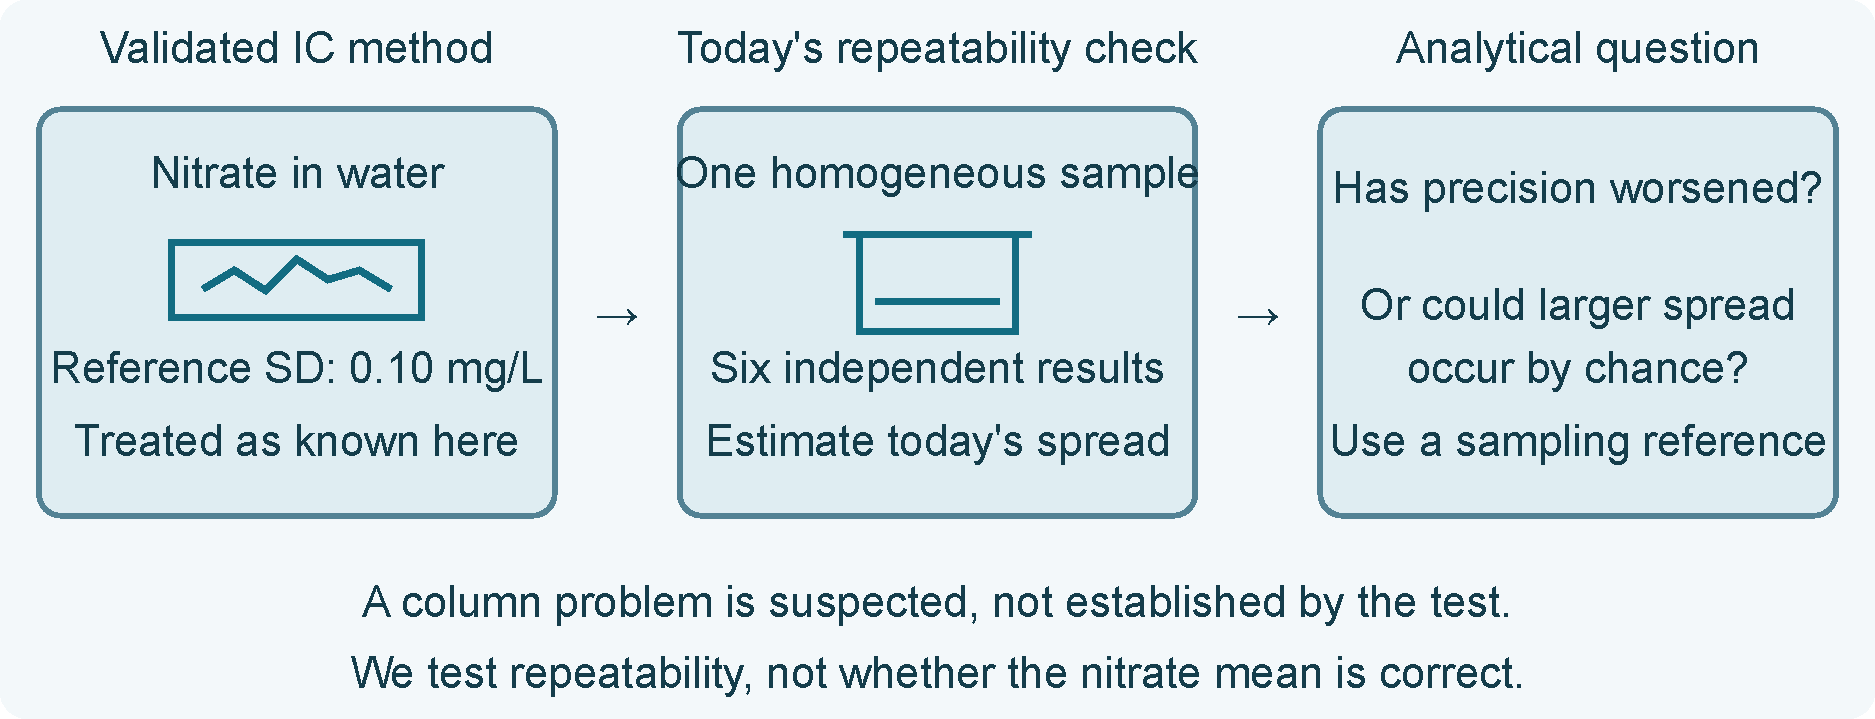
\includegraphics[width=\linewidth,height=.62\textheight,keepaspectratio]{asset-6f6de6c19202c5a754c1227645bc796bc292275ae559cf123671b566775753d2.pdf}\end{center}

\medskip

For a concrete sample, deviations are measured about its fitted sample mean. The six nitrate results in \hyperref[material-a2f73aea1d1bb06d9f7e14786c856e868da67fe8cda1a8bf9d5379cb6f83e00c]{Table~\ref*{material-a2f73aea1d1bb06d9f7e14786c856e868da67fe8cda1a8bf9d5379cb6f83e00c}} have squared deviations summing to 0.12 (mg/L) squared. Dividing by five gives sample variance 0.024 (mg/L) squared, and taking its square root gives sample SD about 0.155 mg/L, as calculated in \hyperref[material-2121e35dd5d78a43d603c22a8ed0c587d0cc000607f3690580a8677934b2fb79]{Eq.~\ref*{material-2121e35dd5d78a43d603c22a8ed0c587d0cc000607f3690580a8677934b2fb79}}. This SD is roughly 55\% above the known reference of 0.10 mg/L. The separate illustrative six-result series in \hyperref[material-bfa445cd83c0f496efbc09ea37a6d18bc6664d9c1883ffad316e6265059e3790]{Fig.~\ref*{material-bfa445cd83c0f496efbc09ea37a6d18bc6664d9c1883ffad316e6265059e3790}} share a mean and have different spreads, showing how sample variance captures variation around the centre. Their sample variances provide the A, B and C reference markers in the repeated-sampling experiment.


\par\medskip
\Needspace{8\baselineskip}
\refstepcounter{scripttable}\label{material-a2f73aea1d1bb06d9f7e14786c856e868da67fe8cda1a8bf9d5379cb6f83e00c}
\noindent\textbf{Table~\ref*{material-a2f73aea1d1bb06d9f7e14786c856e868da67fe8cda1a8bf9d5379cb6f83e00c}.} Six nitrate results, their deviations from the sample mean 10.05 mg/L and their squared deviations.\par\nopagebreak
\begin{longtable}{@{}p{\dimexpr0.333333\linewidth-2\tabcolsep\relax}p{\dimexpr0.333333\linewidth-2\tabcolsep\relax}p{\dimexpr0.333333\linewidth-2\tabcolsep\relax}@{}}
Measurement result (mg/L) & Deviation (mg/L) & Squared deviation ((mg/L)\ensuremath{{}^2}) \\ \hline
\endhead
1: 9.95 & -0.10 & 0.01 \\ \hline
2: 10.15 & +0.10 & 0.01 \\ \hline
3: 9.85 & -0.20 & 0.04 \\ \hline
4: 10.25 & +0.20 & 0.04 \\ \hline
5: 9.95 & -0.10 & 0.01 \\ \hline
6: 10.15 & +0.10 & 0.01 \\ \hline
Sum & 0 & 0.12 \\ \hline
\end{longtable}
\medskip

\par\medskip
\noindent\begin{minipage}{\linewidth}
\refstepcounter{equation}\label{material-2121e35dd5d78a43d603c22a8ed0c587d0cc000607f3690580a8677934b2fb79}
\noindent\textbf{Eq.~\ref*{material-2121e35dd5d78a43d603c22a8ed0c587d0cc000607f3690580a8677934b2fb79}.} Sample variance and standard deviation calculated from the six-result nitrate series.\par\nopagebreak
\begin{center}\begin{adjustbox}{max width=\linewidth}$\displaystyle \begin{gathered}s^2=\frac{\sum_{i=1}^{6}(x_i-\bar x)^2}{6-1}=0.024\;(\mathrm{mg/L})^2\\s\approx0.155\;\mathrm{mg/L},\quad\sigma_0=0.10\;\mathrm{mg/L}\end{gathered}$\end{adjustbox}\end{center}

\par\noindent\textbf{Symbols}

\begin{itemize}\setlength{\itemsep}{1pt}\setlength{\parsep}{0pt}
\item \textbf{i}: Measurement index, from 1 through 6.
\item \textbf{\ensuremath{\Sigma}}: Add all indexed squared deviations.
\item \textbf{\ensuremath{-}, \ensuremath{{}^2}, /}: Subtraction, squaring and division.
\item \textbf{\ensuremath{\sqrt{\vphantom{x}}}}: Positive square root.
\item \textbf{=, \ensuremath{\approx}}: Equality and approximate equality.
\end{itemize}

Estimating one sample mean leaves divisor 6 \ensuremath{-} 1 = 5.

\begin{itemize}\setlength{\itemsep}{1pt}\setlength{\parsep}{0pt}
\item \textbf{\ensuremath{\sigma}\ensuremath{{}_0}}: Reference SD, 0.10 mg/L, known independently.
\end{itemize}

Subscript 0 identifies the reference; the reference value comes from outside this sample.

\begin{itemize}\setlength{\itemsep}{1pt}\setlength{\parsep}{0pt}
\item \textbf{x\ensuremath{{}_i}}: Measurement i (mg/L).
\item \textbf{\ensuremath{\bar{x}}}: Sample mean, 10.05 mg/L; the bar denotes averaging.
\item \textbf{s\ensuremath{{}^2}}: Observed sample variance ((mg/L)\ensuremath{{}^2}).
\item \textbf{s}: Observed sample SD, the positive square root of s\ensuremath{{}^2} (mg/L).
\end{itemize}

\end{minipage}\par
\medskip

\par\medskip
\Needspace{10cm}
\refstepcounter{figure}\label{material-bfa445cd83c0f496efbc09ea37a6d18bc6664d9c1883ffad316e6265059e3790}
\noindent\textbf{Fig.~\ref*{material-bfa445cd83c0f496efbc09ea37a6d18bc6664d9c1883ffad316e6265059e3790}.} Three constructed six-result series share mean 10.000 mg/L. Their sample variances are A: 0.00316, B: 0.00748 and C: 0.01648 (mg/L) squared. Small horizontal offsets separate individual results within each group, including ties.\par\nopagebreak
\begin{center}
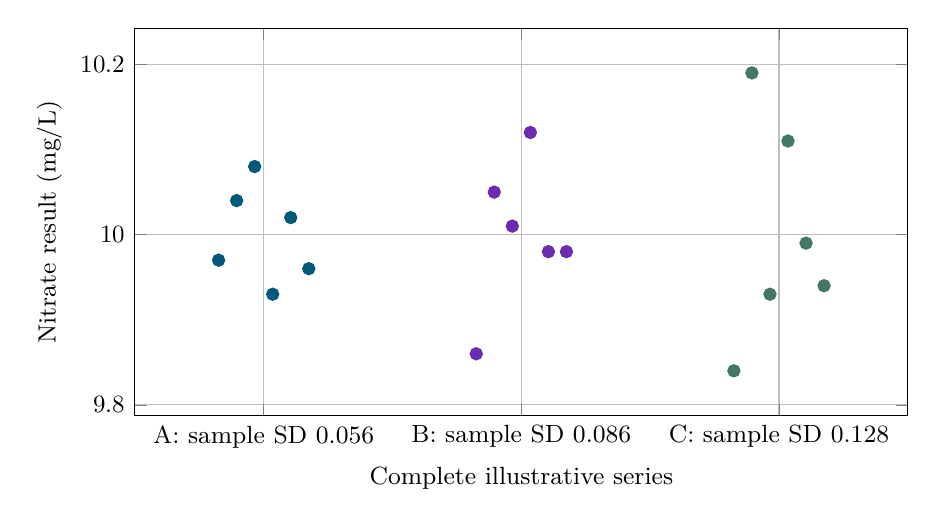
\begin{tikzpicture}
\begin{axis}[width=0.94\linewidth,
height=6.5cm,
scale only axis=false,
grid=major,
tick label style={font=\small},
label style={font=\small},
xlabel={Complete illustrative series},
ylabel={Nitrate result (mg/L)},
legend style={font=\footnotesize,draw=none,at={(0.5,-0.28)},anchor=north,legend columns=1,text width=0.85\linewidth,align=left},
unbounded coords=jump,
scaled ticks=false,
ymin=9.7875,
ymax=10.2425,
xmin=0.5,
xmax=3.5,
xtick={1,2,3},
xticklabels={{A: sample SD 0.056},{B: sample SD 0.086},{C: sample SD 0.128}}]
\addplot[color=pcd1,thick,only marks,mark=*] coordinates {(0.825,9.97) (0.895,10.04) (0.965,10.08) (1.035,9.93) (1.105,10.02) (1.175,9.96)};
\addplot[color=pcd2,thick,only marks,mark=*] coordinates {(1.825,9.86) (1.895,10.05) (1.965,10.01) (2.035,10.12) (2.105,9.98) (2.175,9.98)};
\addplot[color=pcd3,thick,only marks,mark=*] coordinates {(2.825,9.84) (2.895,10.19) (2.965,9.93) (3.035,10.11) (3.105,9.99) (3.175,9.94)};

\end{axis}
\end{tikzpicture}
\end{center}


\medskip

The repeated-sampling experiment holds the population model fixed while generating many complete samples. Each sample contributes one variance estimate to the histogram, which displays the estimator's sampling distribution. Its spread describes the variation among estimates obtained from the same method.


Increasing the number of measurements within each sample concentrates the variance estimates more closely around their target, as compared on the same scale in \hyperref[material-22a5bdb43af90fd3c6b4d2b340af1b6d2f72189ae74b6709a8840f90ffa74cd1]{Fig.~\ref*{material-22a5bdb43af90fd3c6b4d2b340af1b6d2f72189ae74b6709a8840f90ffa74cd1}}. Increasing the number of repeated simulated samples reveals the sampling distribution more clearly. Sample size controls the estimation uncertainty; the number of simulated repetitions controls how clearly that uncertainty is displayed.


\par\medskip
\Needspace{10cm}
\refstepcounter{figure}\label{material-22a5bdb43af90fd3c6b4d2b340af1b6d2f72189ae74b6709a8840f90ffa74cd1}
\noindent\textbf{Fig.~\ref*{material-22a5bdb43af90fd3c6b4d2b340af1b6d2f72189ae74b6709a8840f90ffa74cd1}.} The histograms compare variance estimates from 1,000 Normal series of 6 measurements with 1,000 series of 30 measurements on the same scale. Population SD remains 0.10 mg/L in both experiments. Increasing series size reduces the theoretical relative SD of the variance estimate from 63.25\% to 26.26\%; the simulated six-result series give 61.79\%.\par\nopagebreak
\begin{center}
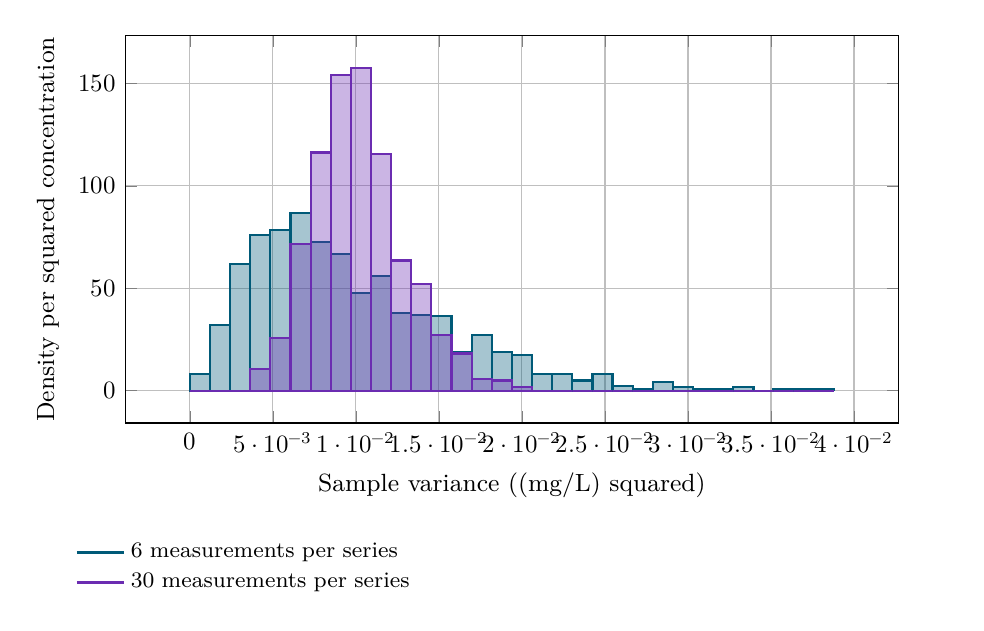
\begin{tikzpicture}
\begin{axis}[width=0.94\linewidth,
height=6.5cm,
scale only axis=false,
grid=major,
tick label style={font=\small},
label style={font=\small},
xlabel={Sample variance ((mg/L) squared)},
ylabel={Density per squared concentration},
legend style={font=\footnotesize,draw=none,at={(0.5,-0.28)},anchor=north,legend columns=1,text width=0.85\linewidth,align=left},
unbounded coords=jump,
scaled ticks=false]
\addplot[color=pcd1,thick,fill=pcd1,fill opacity=0.35,mark=none] coordinates {(0,0) (0,8.249239777400925) (0.0012122329171950297,8.249239777400925) (0.0012122329171950297,0)} \closedcycle;
\addplot[color=pcd1,thick,fill=pcd1,fill opacity=0.35,forget plot,mark=none] coordinates {(0.0012122329171950297,0) (0.0012122329171950297,32.1720351318636) (0.0024244658343900594,32.1720351318636) (0.0024244658343900594,0)} \closedcycle;
\addplot[color=pcd1,thick,fill=pcd1,fill opacity=0.35,forget plot,mark=none] coordinates {(0.0024244658343900594,0) (0.0024244658343900594,61.86929833050693) (0.003636698751585089,61.86929833050693) (0.003636698751585089,0)} \closedcycle;
\addplot[color=pcd1,thick,fill=pcd1,fill opacity=0.35,forget plot,mark=none] coordinates {(0.0036366987515850896,0) (0.0036366987515850896,75.8930059520885) (0.004848931668780119,75.8930059520885) (0.004848931668780119,0)} \closedcycle;
\addplot[color=pcd1,thick,fill=pcd1,fill opacity=0.35,forget plot,mark=none] coordinates {(0.004848931668780119,0) (0.004848931668780119,78.36777788530878) (0.006061164585975148,78.36777788530878) (0.006061164585975148,0)} \closedcycle;
\addplot[color=pcd1,thick,fill=pcd1,fill opacity=0.35,forget plot,mark=none] coordinates {(0.0060611645859751494,0) (0.0060611645859751494,86.6170176627097) (0.007273397503170178,86.6170176627097) (0.007273397503170178,0)} \closedcycle;
\addplot[color=pcd1,thick,fill=pcd1,fill opacity=0.35,forget plot,mark=none] coordinates {(0.007273397503170178,0) (0.007273397503170178,72.59331004112813) (0.008485630420365207,72.59331004112813) (0.008485630420365207,0)} \closedcycle;
\addplot[color=pcd1,thick,fill=pcd1,fill opacity=0.35,forget plot,mark=none] coordinates {(0.008485630420365209,0) (0.008485630420365209,66.81884219694749) (0.009697863337560238,66.81884219694749) (0.009697863337560238,0)} \closedcycle;
\addplot[color=pcd1,thick,fill=pcd1,fill opacity=0.35,forget plot,mark=none] coordinates {(0.009697863337560238,0) (0.009697863337560238,47.845590708925364) (0.010910096254755267,47.845590708925364) (0.010910096254755267,0)} \closedcycle;
\addplot[color=pcd1,thick,fill=pcd1,fill opacity=0.35,forget plot,mark=none] coordinates {(0.010910096254755268,0) (0.010910096254755268,56.09483048632629) (0.012122329171950297,56.09483048632629) (0.012122329171950297,0)} \closedcycle;
\addplot[color=pcd1,thick,fill=pcd1,fill opacity=0.35,forget plot,mark=none] coordinates {(0.012122329171950297,0) (0.012122329171950297,37.94650297604425) (0.013334562089145326,37.94650297604425) (0.013334562089145326,0)} \closedcycle;
\addplot[color=pcd1,thick,fill=pcd1,fill opacity=0.35,forget plot,mark=none] coordinates {(0.013334562089145328,0) (0.013334562089145328,37.12157899830416) (0.014546795006340357,37.12157899830416) (0.014546795006340357,0)} \closedcycle;
\addplot[color=pcd1,thick,fill=pcd1,fill opacity=0.35,forget plot,mark=none] coordinates {(0.014546795006340357,0) (0.014546795006340357,36.29665502056407) (0.015759027923535385,36.29665502056407) (0.015759027923535385,0)} \closedcycle;
\addplot[color=pcd1,thick,fill=pcd1,fill opacity=0.35,forget plot,mark=none] coordinates {(0.015759027923535385,0) (0.015759027923535385,18.973251488022125) (0.016971260840730414,18.973251488022125) (0.016971260840730414,0)} \closedcycle;
\addplot[color=pcd1,thick,fill=pcd1,fill opacity=0.35,forget plot,mark=none] coordinates {(0.016971260840730418,0) (0.016971260840730418,27.222491265423052) (0.018183493757925447,27.222491265423052) (0.018183493757925447,0)} \closedcycle;
\addplot[color=pcd1,thick,fill=pcd1,fill opacity=0.35,forget plot,mark=none] coordinates {(0.018183493757925447,0) (0.018183493757925447,18.973251488022125) (0.019395726675120475,18.973251488022125) (0.019395726675120475,0)} \closedcycle;
\addplot[color=pcd1,thick,fill=pcd1,fill opacity=0.35,forget plot,mark=none] coordinates {(0.019395726675120475,0) (0.019395726675120475,17.323403532541942) (0.020607959592315504,17.323403532541942) (0.020607959592315504,0)} \closedcycle;
\addplot[color=pcd1,thick,fill=pcd1,fill opacity=0.35,forget plot,mark=none] coordinates {(0.020607959592315504,0) (0.020607959592315504,8.249239777400925) (0.021820192509510533,8.249239777400925) (0.021820192509510533,0)} \closedcycle;
\addplot[color=pcd1,thick,fill=pcd1,fill opacity=0.35,forget plot,mark=none] coordinates {(0.021820192509510537,0) (0.021820192509510537,8.249239777400925) (0.023032425426705565,8.249239777400925) (0.023032425426705565,0)} \closedcycle;
\addplot[color=pcd1,thick,fill=pcd1,fill opacity=0.35,forget plot,mark=none] coordinates {(0.023032425426705565,0) (0.023032425426705565,4.949543866440555) (0.024244658343900594,4.949543866440555) (0.024244658343900594,0)} \closedcycle;
\addplot[color=pcd1,thick,fill=pcd1,fill opacity=0.35,forget plot,mark=none] coordinates {(0.024244658343900594,0) (0.024244658343900594,8.249239777400925) (0.025456891261095623,8.249239777400925) (0.025456891261095623,0)} \closedcycle;
\addplot[color=pcd1,thick,fill=pcd1,fill opacity=0.35,forget plot,mark=none] coordinates {(0.025456891261095623,0) (0.025456891261095623,2.4747719332202776) (0.026669124178290652,2.4747719332202776) (0.026669124178290652,0)} \closedcycle;
\addplot[color=pcd1,thick,fill=pcd1,fill opacity=0.35,forget plot,mark=none] coordinates {(0.026669124178290655,0) (0.026669124178290655,0.8249239777400924) (0.027881357095485684,0.8249239777400924) (0.027881357095485684,0)} \closedcycle;
\addplot[color=pcd1,thick,fill=pcd1,fill opacity=0.35,forget plot,mark=none] coordinates {(0.027881357095485684,0) (0.027881357095485684,4.124619888700463) (0.029093590012680713,4.124619888700463) (0.029093590012680713,0)} \closedcycle;
\addplot[color=pcd1,thick,fill=pcd1,fill opacity=0.35,forget plot,mark=none] coordinates {(0.029093590012680713,0) (0.029093590012680713,1.6498479554801848) (0.030305822929875742,1.6498479554801848) (0.030305822929875742,0)} \closedcycle;
\addplot[color=pcd1,thick,fill=pcd1,fill opacity=0.35,forget plot,mark=none] coordinates {(0.030305822929875742,0) (0.030305822929875742,0.8249239777400924) (0.03151805584707077,0.8249239777400924) (0.03151805584707077,0)} \closedcycle;
\addplot[color=pcd1,thick,fill=pcd1,fill opacity=0.35,forget plot,mark=none] coordinates {(0.03151805584707077,0) (0.03151805584707077,0.8249239777400924) (0.03273028876426581,0.8249239777400924) (0.03273028876426581,0)} \closedcycle;
\addplot[color=pcd1,thick,fill=pcd1,fill opacity=0.35,forget plot,mark=none] coordinates {(0.0327302887642658,0) (0.0327302887642658,1.6498479554801848) (0.033942521681460835,1.6498479554801848) (0.033942521681460835,0)} \closedcycle;
\addplot[color=pcd1,thick,fill=pcd1,fill opacity=0.35,forget plot,mark=none] coordinates {(0.03394252168146083,0) (0.03394252168146083,0) (0.035154754598655864,0) (0.035154754598655864,0)} \closedcycle;
\addplot[color=pcd1,thick,fill=pcd1,fill opacity=0.35,forget plot,mark=none] coordinates {(0.03515475459865586,0) (0.03515475459865586,0.8249239777400924) (0.03636698751585089,0.8249239777400924) (0.03636698751585089,0)} \closedcycle;
\addplot[color=pcd1,thick,fill=pcd1,fill opacity=0.35,forget plot,mark=none] coordinates {(0.036366987515850886,0) (0.036366987515850886,0.8249239777400924) (0.03757922043304592,0.8249239777400924) (0.03757922043304592,0)} \closedcycle;
\addplot[color=pcd1,thick,fill=pcd1,fill opacity=0.35,forget plot,mark=none] coordinates {(0.037579220433045915,0) (0.037579220433045915,0.8249239777400924) (0.03879145335024095,0.8249239777400924) (0.03879145335024095,0)} \closedcycle;
\addlegendentry{6 measurements per series}
\addplot[color=pcd2,thick,fill=pcd2,fill opacity=0.35,mark=none] coordinates {(0,0) (0,0) (0.0012122329171950297,0) (0.0012122329171950297,0)} \closedcycle;
\addplot[color=pcd2,thick,fill=pcd2,fill opacity=0.35,forget plot,mark=none] coordinates {(0.0012122329171950297,0) (0.0012122329171950297,0) (0.0024244658343900594,0) (0.0024244658343900594,0)} \closedcycle;
\addplot[color=pcd2,thick,fill=pcd2,fill opacity=0.35,forget plot,mark=none] coordinates {(0.0024244658343900594,0) (0.0024244658343900594,0) (0.003636698751585089,0) (0.003636698751585089,0)} \closedcycle;
\addplot[color=pcd2,thick,fill=pcd2,fill opacity=0.35,forget plot,mark=none] coordinates {(0.0036366987515850896,0) (0.0036366987515850896,10.724011710621202) (0.004848931668780119,10.724011710621202) (0.004848931668780119,0)} \closedcycle;
\addplot[color=pcd2,thick,fill=pcd2,fill opacity=0.35,forget plot,mark=none] coordinates {(0.004848931668780119,0) (0.004848931668780119,25.572643309942865) (0.006061164585975148,25.572643309942865) (0.006061164585975148,0)} \closedcycle;
\addplot[color=pcd2,thick,fill=pcd2,fill opacity=0.35,forget plot,mark=none] coordinates {(0.0060611645859751494,0) (0.0060611645859751494,71.76838606338804) (0.007273397503170178,71.76838606338804) (0.007273397503170178,0)} \closedcycle;
\addplot[color=pcd2,thick,fill=pcd2,fill opacity=0.35,forget plot,mark=none] coordinates {(0.007273397503170178,0) (0.007273397503170178,116.31428086135303) (0.008485630420365207,116.31428086135303) (0.008485630420365207,0)} \closedcycle;
\addplot[color=pcd2,thick,fill=pcd2,fill opacity=0.35,forget plot,mark=none] coordinates {(0.008485630420365209,0) (0.008485630420365209,154.26078383739727) (0.009697863337560238,154.26078383739727) (0.009697863337560238,0)} \closedcycle;
\addplot[color=pcd2,thick,fill=pcd2,fill opacity=0.35,forget plot,mark=none] coordinates {(0.009697863337560238,0) (0.009697863337560238,157.56047974835766) (0.010910096254755267,157.56047974835766) (0.010910096254755267,0)} \closedcycle;
\addplot[color=pcd2,thick,fill=pcd2,fill opacity=0.35,forget plot,mark=none] coordinates {(0.010910096254755268,0) (0.010910096254755268,115.48935688361296) (0.012122329171950297,115.48935688361296) (0.012122329171950297,0)} \closedcycle;
\addplot[color=pcd2,thick,fill=pcd2,fill opacity=0.35,forget plot,mark=none] coordinates {(0.012122329171950297,0) (0.012122329171950297,63.51914628598712) (0.013334562089145326,63.51914628598712) (0.013334562089145326,0)} \closedcycle;
\addplot[color=pcd2,thick,fill=pcd2,fill opacity=0.35,forget plot,mark=none] coordinates {(0.013334562089145328,0) (0.013334562089145328,51.97021059762582) (0.014546795006340357,51.97021059762582) (0.014546795006340357,0)} \closedcycle;
\addplot[color=pcd2,thick,fill=pcd2,fill opacity=0.35,forget plot,mark=none] coordinates {(0.014546795006340357,0) (0.014546795006340357,27.222491265423052) (0.015759027923535385,27.222491265423052) (0.015759027923535385,0)} \closedcycle;
\addplot[color=pcd2,thick,fill=pcd2,fill opacity=0.35,forget plot,mark=none] coordinates {(0.015759027923535385,0) (0.015759027923535385,18.148327510282034) (0.016971260840730414,18.148327510282034) (0.016971260840730414,0)} \closedcycle;
\addplot[color=pcd2,thick,fill=pcd2,fill opacity=0.35,forget plot,mark=none] coordinates {(0.016971260840730418,0) (0.016971260840730418,5.774467844180647) (0.018183493757925447,5.774467844180647) (0.018183493757925447,0)} \closedcycle;
\addplot[color=pcd2,thick,fill=pcd2,fill opacity=0.35,forget plot,mark=none] coordinates {(0.018183493757925447,0) (0.018183493757925447,4.949543866440555) (0.019395726675120475,4.949543866440555) (0.019395726675120475,0)} \closedcycle;
\addplot[color=pcd2,thick,fill=pcd2,fill opacity=0.35,forget plot,mark=none] coordinates {(0.019395726675120475,0) (0.019395726675120475,1.6498479554801848) (0.020607959592315504,1.6498479554801848) (0.020607959592315504,0)} \closedcycle;
\addplot[color=pcd2,thick,fill=pcd2,fill opacity=0.35,forget plot,mark=none] coordinates {(0.020607959592315504,0) (0.020607959592315504,0) (0.021820192509510533,0) (0.021820192509510533,0)} \closedcycle;
\addplot[color=pcd2,thick,fill=pcd2,fill opacity=0.35,forget plot,mark=none] coordinates {(0.021820192509510537,0) (0.021820192509510537,0) (0.023032425426705565,0) (0.023032425426705565,0)} \closedcycle;
\addplot[color=pcd2,thick,fill=pcd2,fill opacity=0.35,forget plot,mark=none] coordinates {(0.023032425426705565,0) (0.023032425426705565,0) (0.024244658343900594,0) (0.024244658343900594,0)} \closedcycle;
\addplot[color=pcd2,thick,fill=pcd2,fill opacity=0.35,forget plot,mark=none] coordinates {(0.024244658343900594,0) (0.024244658343900594,0) (0.025456891261095623,0) (0.025456891261095623,0)} \closedcycle;
\addplot[color=pcd2,thick,fill=pcd2,fill opacity=0.35,forget plot,mark=none] coordinates {(0.025456891261095623,0) (0.025456891261095623,0) (0.026669124178290652,0) (0.026669124178290652,0)} \closedcycle;
\addplot[color=pcd2,thick,fill=pcd2,fill opacity=0.35,forget plot,mark=none] coordinates {(0.026669124178290655,0) (0.026669124178290655,0) (0.027881357095485684,0) (0.027881357095485684,0)} \closedcycle;
\addplot[color=pcd2,thick,fill=pcd2,fill opacity=0.35,forget plot,mark=none] coordinates {(0.027881357095485684,0) (0.027881357095485684,0) (0.029093590012680713,0) (0.029093590012680713,0)} \closedcycle;
\addplot[color=pcd2,thick,fill=pcd2,fill opacity=0.35,forget plot,mark=none] coordinates {(0.029093590012680713,0) (0.029093590012680713,0) (0.030305822929875742,0) (0.030305822929875742,0)} \closedcycle;
\addplot[color=pcd2,thick,fill=pcd2,fill opacity=0.35,forget plot,mark=none] coordinates {(0.030305822929875742,0) (0.030305822929875742,0) (0.03151805584707077,0) (0.03151805584707077,0)} \closedcycle;
\addplot[color=pcd2,thick,fill=pcd2,fill opacity=0.35,forget plot,mark=none] coordinates {(0.03151805584707077,0) (0.03151805584707077,0) (0.03273028876426581,0) (0.03273028876426581,0)} \closedcycle;
\addplot[color=pcd2,thick,fill=pcd2,fill opacity=0.35,forget plot,mark=none] coordinates {(0.0327302887642658,0) (0.0327302887642658,0) (0.033942521681460835,0) (0.033942521681460835,0)} \closedcycle;
\addplot[color=pcd2,thick,fill=pcd2,fill opacity=0.35,forget plot,mark=none] coordinates {(0.03394252168146083,0) (0.03394252168146083,0) (0.035154754598655864,0) (0.035154754598655864,0)} \closedcycle;
\addplot[color=pcd2,thick,fill=pcd2,fill opacity=0.35,forget plot,mark=none] coordinates {(0.03515475459865586,0) (0.03515475459865586,0) (0.03636698751585089,0) (0.03636698751585089,0)} \closedcycle;
\addplot[color=pcd2,thick,fill=pcd2,fill opacity=0.35,forget plot,mark=none] coordinates {(0.036366987515850886,0) (0.036366987515850886,0) (0.03757922043304592,0) (0.03757922043304592,0)} \closedcycle;
\addplot[color=pcd2,thick,fill=pcd2,fill opacity=0.35,forget plot,mark=none] coordinates {(0.037579220433045915,0) (0.037579220433045915,0) (0.03879145335024095,0) (0.03879145335024095,0)} \closedcycle;
\addlegendentry{30 measurements per series}

\end{axis}
\end{tikzpicture}
\end{center}

% Full-precision experiment details: {"blockId":"ex:p1-n41-v--block","parameters":[{"key":"n","label":"Measurements per complete series","value":6},{"key":"sigma","label":"True method SD (mg/L), assumed","value":0.1},{"key":"M","label":"Simulated complete series","value":1000},{"key":"seed","label":"Replay seed (Park-Miller)","value":20261102},{"key":"observed","label":"Observed QC variance ((mg/L) squared)","value":0.024},{"key":"comparisonN","label":"Comparison measurements per series","value":30}],"readouts":[{"label":"Complete series","value":1000},{"label":"Measurements per series","value":6},{"label":"Mean estimated variance","value":0.009791547543033078},{"label":"Relative SD of variance estimates","value":0.6178852173778371},{"label":"Theoretical relative SD","value":0.6324555320336759},{"label":"Observed variance","value":0.024},{"label":"Simulated fraction at least observed","value":0.029},{"label":"Comparison measurements per series","value":30},{"label":"Comparison theoretical relative SD","value":0.2626128657194451}],"note":"The true method SD stays fixed. More simulated series reveal the sampling distribution more clearly; more measurements per series improve the variance estimate. The histogram includes the sample variance from every simulated series.","markers":[[]]}

\medskip

An unchanged population model therefore produces a distribution of variance estimates (\hyperref[material-03922b0485ba5e327df5b19a518a98d007e83690677077f5db1ae907b0e17142]{Fig.~\ref*{material-03922b0485ba5e327df5b19a518a98d007e83690677077f5db1ae907b0e17142}}). The relative uncertainty in \hyperref[material-db58b1a6fdbebf9a49b1cd134b0caccf7e12793f0759b34d27bd3d38161f990e]{Eq.~\ref*{material-db58b1a6fdbebf9a49b1cd134b0caccf7e12793f0759b34d27bd3d38161f990e}} quantifies the sample-size effect, and \hyperref[material-3076e5fcc52fc73d5ca5d8b5387f7bfaf559a150a4d0a9996d07cca4d30273b9]{Listing~\ref*{material-3076e5fcc52fc73d5ca5d8b5387f7bfaf559a150a4d0a9996d07cca4d30273b9}} reproduces the repeated-sampling calculation in R. Under independent Normal sampling, scaled sample variances have a chi-square distribution. This relationship provides a mathematical reference for evaluating precision and, later, for comparing two estimated variances. Its justification follows from the stated population model and the independence of the measurements.


\par\medskip
\noindent\begin{minipage}{\linewidth}
\refstepcounter{equation}\label{material-db58b1a6fdbebf9a49b1cd134b0caccf7e12793f0759b34d27bd3d38161f990e}
\noindent\textbf{Eq.~\ref*{material-db58b1a6fdbebf9a49b1cd134b0caccf7e12793f0759b34d27bd3d38161f990e}.} Relative sampling uncertainty of the variance estimate under independent Normal sampling.\par\nopagebreak
\begin{center}\begin{adjustbox}{max width=\linewidth}$\displaystyle \begin{gathered}E(Q)=n-1,\quad\operatorname{Var}(Q)=2(n-1)\\\operatorname{Var}(S^2)=\frac{2\sigma^4}{n-1},\quad\frac{\operatorname{SD}(S^2)}{E(S^2)}=\sqrt{\frac{2}{n-1}}\end{gathered}$\end{adjustbox}\end{center}

\par\noindent\textbf{Symbols}

\begin{itemize}\setlength{\itemsep}{1pt}\setlength{\parsep}{0pt}
\item \textbf{n}: Number of independent Normal measurement results, at least two.
\item \textbf{S\ensuremath{{}^2}}: Random sample variance ((mg/L)\ensuremath{{}^2}).
\item \textbf{\ensuremath{\sigma}}: True population SD (mg/L).
\item \textbf{Q}: Centred squared sum divided by true variance (dimensionless).
\item \textbf{E}: Expectation; E(S\ensuremath{{}^2}) has units (mg/L)\ensuremath{{}^2}.
\item \textbf{Var}: Variance; Var(S\ensuremath{{}^2}) has units (mg/L)\ensuremath{{}^4}.
\item \textbf{SD}: Positive square root of variance; SD(S\ensuremath{{}^2}) has units (mg/L)\ensuremath{{}^2}.
\item \textbf{n \ensuremath{-} 1}: Degrees of freedom after estimating one mean.
\item \textbf{Powers, \ensuremath{\sqrt{\vphantom{x}}}, /, =}: Exponentiation, positive square root, division and equality; adjacent factors multiply.
\end{itemize}

SD(S\ensuremath{{}^2}) / E(S\ensuremath{{}^2}) is a dimensionless relative SD, displayed as a percentage. The QC statistic has this reference law at \ensuremath{\sigma} = \ensuremath{\sigma}\ensuremath{{}_0}.

\end{minipage}\par
\medskip

\par\medskip
\Needspace{10cm}
\refstepcounter{figure}\label{material-03922b0485ba5e327df5b19a518a98d007e83690677077f5db1ae907b0e17142}
\noindent\textbf{Fig.~\ref*{material-03922b0485ba5e327df5b19a518a98d007e83690677077f5db1ae907b0e17142}.} Each histogram entry is the variance of one complete six-result Normal sample, calculated about that sample's fitted mean. All 1,000 repetitions use population SD 0.10 mg/L. The estimated variances average 0.009792 (mg/L) squared, with empirical relative SD 61.79\%, compared with the theoretical 63.25\%. In this simulation, 2.9\% of estimates reach or exceed the observed variance of 0.024 (mg/L) squared.\par\nopagebreak
\begin{center}
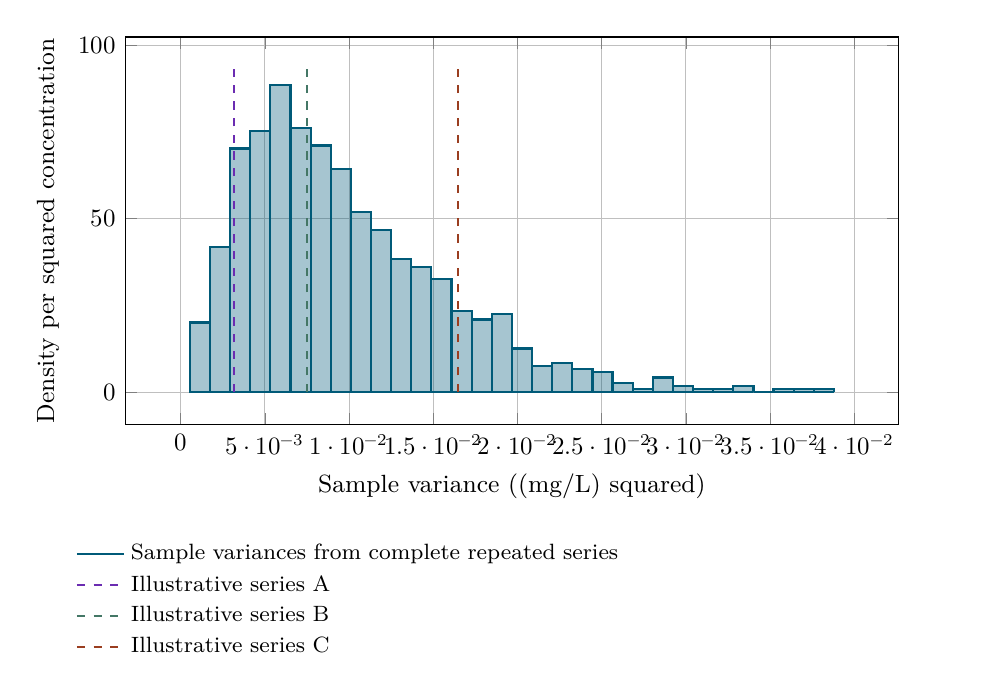
\begin{tikzpicture}
\begin{axis}[width=0.94\linewidth,
height=6.5cm,
scale only axis=false,
grid=major,
tick label style={font=\small},
label style={font=\small},
xlabel={Sample variance ((mg/L) squared)},
ylabel={Density per squared concentration},
legend style={font=\footnotesize,draw=none,at={(0.5,-0.28)},anchor=north,legend columns=1,text width=0.85\linewidth,align=left},
unbounded coords=jump,
scaled ticks=false]
\addplot[color=pcd1,thick,fill=pcd1,fill opacity=0.35,mark=none] coordinates {(0.0005434685114807966,0) (0.0005434685114807966,20.07948923943611) (0.0017387180376920515,20.07948923943611) (0.0017387180376920515,0)} \closedcycle;
\addplot[color=pcd1,thick,fill=pcd1,fill opacity=0.35,forget plot,mark=none] coordinates {(0.0017387180376920515,0) (0.0017387180376920515,41.83226924882523) (0.0029339675639033064,41.83226924882523) (0.0029339675639033064,0)} \closedcycle;
\addplot[color=pcd1,thick,fill=pcd1,fill opacity=0.35,forget plot,mark=none] coordinates {(0.0029339675639033064,0) (0.0029339675639033064,70.27821233802638) (0.004129217090114561,70.27821233802638) (0.004129217090114561,0)} \closedcycle;
\addplot[color=pcd1,thick,fill=pcd1,fill opacity=0.35,forget plot,mark=none] coordinates {(0.004129217090114563,0) (0.004129217090114563,75.2980846478854) (0.005324466616325817,75.2980846478854) (0.005324466616325817,0)} \closedcycle;
\addplot[color=pcd1,thick,fill=pcd1,fill opacity=0.35,forget plot,mark=none] coordinates {(0.005324466616325817,0) (0.005324466616325817,88.68441080750948) (0.006519716142537071,88.68441080750948) (0.006519716142537071,0)} \closedcycle;
\addplot[color=pcd1,thick,fill=pcd1,fill opacity=0.35,forget plot,mark=none] coordinates {(0.0065197161425370725,0) (0.0065197161425370725,76.13473003286191) (0.0077149656687483265,76.13473003286191) (0.0077149656687483265,0)} \closedcycle;
\addplot[color=pcd1,thick,fill=pcd1,fill opacity=0.35,forget plot,mark=none] coordinates {(0.0077149656687483265,0) (0.0077149656687483265,71.11485772300288) (0.00891021519495958,71.11485772300288) (0.00891021519495958,0)} \closedcycle;
\addplot[color=pcd1,thick,fill=pcd1,fill opacity=0.35,forget plot,mark=none] coordinates {(0.008910215194959582,0) (0.008910215194959582,64.42169464319085) (0.010105464721170836,64.42169464319085) (0.010105464721170836,0)} \closedcycle;
\addplot[color=pcd1,thick,fill=pcd1,fill opacity=0.35,forget plot,mark=none] coordinates {(0.010105464721170836,0) (0.010105464721170836,51.87201386854328) (0.01130071424738209,51.87201386854328) (0.01130071424738209,0)} \closedcycle;
\addplot[color=pcd1,thick,fill=pcd1,fill opacity=0.35,forget plot,mark=none] coordinates {(0.011300714247382092,0) (0.011300714247382092,46.85214155868425) (0.012495963773593346,46.85214155868425) (0.012495963773593346,0)} \closedcycle;
\addplot[color=pcd1,thick,fill=pcd1,fill opacity=0.35,forget plot,mark=none] coordinates {(0.012495963773593346,0) (0.012495963773593346,38.48568770891921) (0.0136912132998046,38.48568770891921) (0.0136912132998046,0)} \closedcycle;
\addplot[color=pcd1,thick,fill=pcd1,fill opacity=0.35,forget plot,mark=none] coordinates {(0.013691213299804602,0) (0.013691213299804602,35.97575155398969) (0.014886462826015856,35.97575155398969) (0.014886462826015856,0)} \closedcycle;
\addplot[color=pcd1,thick,fill=pcd1,fill opacity=0.35,forget plot,mark=none] coordinates {(0.014886462826015856,0) (0.014886462826015856,32.62917001408368) (0.01608171235222711,32.62917001408368) (0.01608171235222711,0)} \closedcycle;
\addplot[color=pcd1,thick,fill=pcd1,fill opacity=0.35,forget plot,mark=none] coordinates {(0.01608171235222711,0) (0.01608171235222711,23.426070779342126) (0.017276961878438368,23.426070779342126) (0.017276961878438368,0)} \closedcycle;
\addplot[color=pcd1,thick,fill=pcd1,fill opacity=0.35,forget plot,mark=none] coordinates {(0.017276961878438364,0) (0.017276961878438364,20.916134624412614) (0.01847221140464962,20.916134624412614) (0.01847221140464962,0)} \closedcycle;
\addplot[color=pcd1,thick,fill=pcd1,fill opacity=0.35,forget plot,mark=none] coordinates {(0.018472211404649618,0) (0.018472211404649618,22.589425394365623) (0.019667460930860876,22.589425394365623) (0.019667460930860876,0)} \closedcycle;
\addplot[color=pcd1,thick,fill=pcd1,fill opacity=0.35,forget plot,mark=none] coordinates {(0.019667460930860876,0) (0.019667460930860876,12.549680774647568) (0.020862710457072133,12.549680774647568) (0.020862710457072133,0)} \closedcycle;
\addplot[color=pcd1,thick,fill=pcd1,fill opacity=0.35,forget plot,mark=none] coordinates {(0.02086271045707213,0) (0.02086271045707213,7.52980846478854) (0.022057959983283387,7.52980846478854) (0.022057959983283387,0)} \closedcycle;
\addplot[color=pcd1,thick,fill=pcd1,fill opacity=0.35,forget plot,mark=none] coordinates {(0.022057959983283384,0) (0.022057959983283384,8.366453849765046) (0.02325320950949464,8.366453849765046) (0.02325320950949464,0)} \closedcycle;
\addplot[color=pcd1,thick,fill=pcd1,fill opacity=0.35,forget plot,mark=none] coordinates {(0.023253209509494638,0) (0.023253209509494638,6.693163079812036) (0.024448459035705895,6.693163079812036) (0.024448459035705895,0)} \closedcycle;
\addplot[color=pcd1,thick,fill=pcd1,fill opacity=0.35,forget plot,mark=none] coordinates {(0.024448459035705895,0) (0.024448459035705895,5.8565176948355315) (0.025643708561917153,5.8565176948355315) (0.025643708561917153,0)} \closedcycle;
\addplot[color=pcd1,thick,fill=pcd1,fill opacity=0.35,forget plot,mark=none] coordinates {(0.02564370856191715,0) (0.02564370856191715,2.509936154929514) (0.026838958088128407,2.509936154929514) (0.026838958088128407,0)} \closedcycle;
\addplot[color=pcd1,thick,fill=pcd1,fill opacity=0.35,forget plot,mark=none] coordinates {(0.026838958088128403,0) (0.026838958088128403,0.8366453849765045) (0.02803420761433966,0.8366453849765045) (0.02803420761433966,0)} \closedcycle;
\addplot[color=pcd1,thick,fill=pcd1,fill opacity=0.35,forget plot,mark=none] coordinates {(0.028034207614339657,0) (0.028034207614339657,4.183226924882523) (0.029229457140550915,4.183226924882523) (0.029229457140550915,0)} \closedcycle;
\addplot[color=pcd1,thick,fill=pcd1,fill opacity=0.35,forget plot,mark=none] coordinates {(0.029229457140550915,0) (0.029229457140550915,1.673290769953009) (0.030424706666762173,1.673290769953009) (0.030424706666762173,0)} \closedcycle;
\addplot[color=pcd1,thick,fill=pcd1,fill opacity=0.35,forget plot,mark=none] coordinates {(0.03042470666676217,0) (0.03042470666676217,0.8366453849765045) (0.03161995619297343,0.8366453849765045) (0.03161995619297343,0)} \closedcycle;
\addplot[color=pcd1,thick,fill=pcd1,fill opacity=0.35,forget plot,mark=none] coordinates {(0.03161995619297343,0) (0.03161995619297343,0.8366453849765045) (0.03281520571918468,0.8366453849765045) (0.03281520571918468,0)} \closedcycle;
\addplot[color=pcd1,thick,fill=pcd1,fill opacity=0.35,forget plot,mark=none] coordinates {(0.03281520571918468,0) (0.03281520571918468,1.673290769953009) (0.03401045524539593,1.673290769953009) (0.03401045524539593,0)} \closedcycle;
\addplot[color=pcd1,thick,fill=pcd1,fill opacity=0.35,forget plot,mark=none] coordinates {(0.034010455245395935,0) (0.034010455245395935,0) (0.035205704771607185,0) (0.035205704771607185,0)} \closedcycle;
\addplot[color=pcd1,thick,fill=pcd1,fill opacity=0.35,forget plot,mark=none] coordinates {(0.035205704771607185,0) (0.035205704771607185,0.8366453849765045) (0.036400954297818436,0.8366453849765045) (0.036400954297818436,0)} \closedcycle;
\addplot[color=pcd1,thick,fill=pcd1,fill opacity=0.35,forget plot,mark=none] coordinates {(0.03640095429781844,0) (0.03640095429781844,0.8366453849765045) (0.03759620382402969,0.8366453849765045) (0.03759620382402969,0)} \closedcycle;
\addplot[color=pcd1,thick,fill=pcd1,fill opacity=0.35,forget plot,mark=none] coordinates {(0.0375962038240297,0) (0.0375962038240297,0.8366453849765045) (0.03879145335024095,0.8366453849765045) (0.03879145335024095,0)} \closedcycle;
\addlegendentry{Sample variances from complete repeated series}
\addplot[color=pcd2,dashed,thick] coordinates {(0.00316,0) (0.00316,93.11863134788496)};
\addlegendentry{Illustrative series A}
\addplot[color=pcd3,dashed,thick] coordinates {(0.00748,0) (0.00748,93.11863134788496)};
\addlegendentry{Illustrative series B}
\addplot[color=pcd4,dashed,thick] coordinates {(0.01648,0) (0.01648,93.11863134788496)};
\addlegendentry{Illustrative series C}
\end{axis}
\end{tikzpicture}
\end{center}

% Full-precision experiment details: {"blockId":"ex:rv-variance-v--block","parameters":[{"key":"n","label":"Measurements per complete series","value":6},{"key":"sigma","label":"True method SD (mg/L), assumed","value":0.1},{"key":"M","label":"Simulated complete series","value":1000},{"key":"seed","label":"Replay seed (Park-Miller)","value":20261102},{"key":"observed","label":"Observed QC variance ((mg/L) squared)","value":0.024}],"readouts":[{"label":"Complete series","value":1000},{"label":"Measurements per series","value":6},{"label":"Mean estimated variance","value":0.009791547543033078},{"label":"Relative SD of variance estimates","value":0.6178852173778371},{"label":"Theoretical relative SD","value":0.6324555320336759},{"label":"Observed variance","value":0.024},{"label":"Simulated fraction at least observed","value":0.029}],"note":"The true method SD stays fixed. More simulated series reveal the sampling distribution more clearly; more measurements per series improve the variance estimate. The histogram includes the sample variance from every simulated series.","markers":[[{"x":0.00316,"label":"Illustrative series A"},{"x":0.00748,"label":"Illustrative series B"},{"x":0.01648,"label":"Illustrative series C"}]]}

\medskip

\par\medskip
\Needspace{8\baselineskip}
\refstepcounter{listing}\label{material-3076e5fcc52fc73d5ca5d8b5387f7bfaf559a150a4d0a9996d07cca4d30273b9}
\noindent\textbf{Listing~\ref*{material-3076e5fcc52fc73d5ca5d8b5387f7bfaf559a150a4d0a9996d07cca4d30273b9}.} R reproduction of repeated complete samples and their variance estimates.\par\nopagebreak
\begin{Verbatim}[fontsize=\footnotesize,breaklines=true,breakanywhere=true]
# Hypothetical stable method. No field or validation data.
# First change M: 100, 1000, 10000. Later change n: 6, 30.
M <- 100; n <- 6; sigma <- 0.10; mu <- 10
stopifnot(M %in% c(100, 1000, 10000), n >= 2, n <= 100,
          n == as.integer(n), sigma > 0)
state <- 20261101
S2 <- numeric(M)
first <- numeric(n)
for (j in seq_len(M)) {
  x <- numeric(n)
  for (i in seq_len(n)) {
    state <- (16807 * state) %% 2147483647
    x[i] <- mu + sigma * qnorm(state / 2147483647)
  }
  if (j == 1) first <- x
  S2[j] <- sum((x - mean(x))^2) / (n - 1)
}
cat('First series (mg/L):', format(first, digits=8), '\n')
cat('M:', M, 'n:', n, 'df:', n-1, '\n')
cat('Mean sample variance:', mean(S2), '(mg/L)^2\n')
cat('Relative SD, empirical:', sd(S2)/mean(S2),
    'theoretical:', sqrt(2/(n-1)), '\n')
cat('Count at least observed variance 0.024:', sum(S2 >= 0.024), '\n')
old <- par(mfrow=c(1,2), mar=c(5,4,3,1))
plot(seq_len(M), S2, pch=16, cex=0.35, col='#176b90',
     xlab='Independent series number', ylab='Sample variance ((mg/L)^2)',
     main=paste(M, 'complete series'), ylim=c(0,max(0.064,S2)))
abline(h=sigma^2, col='#a63d21', lty=2)
breaks <- seq(0, max(0.064, ceiling(max(S2)/0.002)*0.002), by=0.002)
hist(S2, breaks=breaks, right=FALSE, probability=TRUE, col='#8ecae6',
     xlab='Sample variance ((mg/L)^2)', ylab='Density per (mg/L)^2',
     main=paste('n =', n), xlim=c(0,max(breaks)))
abline(v=0.024, col='#a63d21', lwd=2)
par(old)

\end{Verbatim}

\medskip

\clearpage
\section{Squared Normal components and the chi-square reference}
Squaring a standard-Normal value turns positive and negative deviations into nonnegative squared distances (\hyperref[material-148addcd765d7d358808157643aea1b444b8b44ba741df6ae255133980c0c87f]{Fig.~\ref*{material-148addcd765d7d358808157643aea1b444b8b44ba741df6ae255133980c0c87f}}). This produces a chi-square variable with one degree of freedom. Large original deviations become especially large squares, producing a long right tail.


\par\medskip
\Needspace{10cm}
\refstepcounter{figure}\label{material-148addcd765d7d358808157643aea1b444b8b44ba741df6ae255133980c0c87f}
\noindent\textbf{Fig.~\ref*{material-148addcd765d7d358808157643aea1b444b8b44ba741df6ae255133980c0c87f}.} Squaring maps both signs of a standard-Normal value to the same nonnegative squared distance. The symmetric Normal density becomes a one-degree-of-freedom chi-square density.\par\nopagebreak
\begin{center}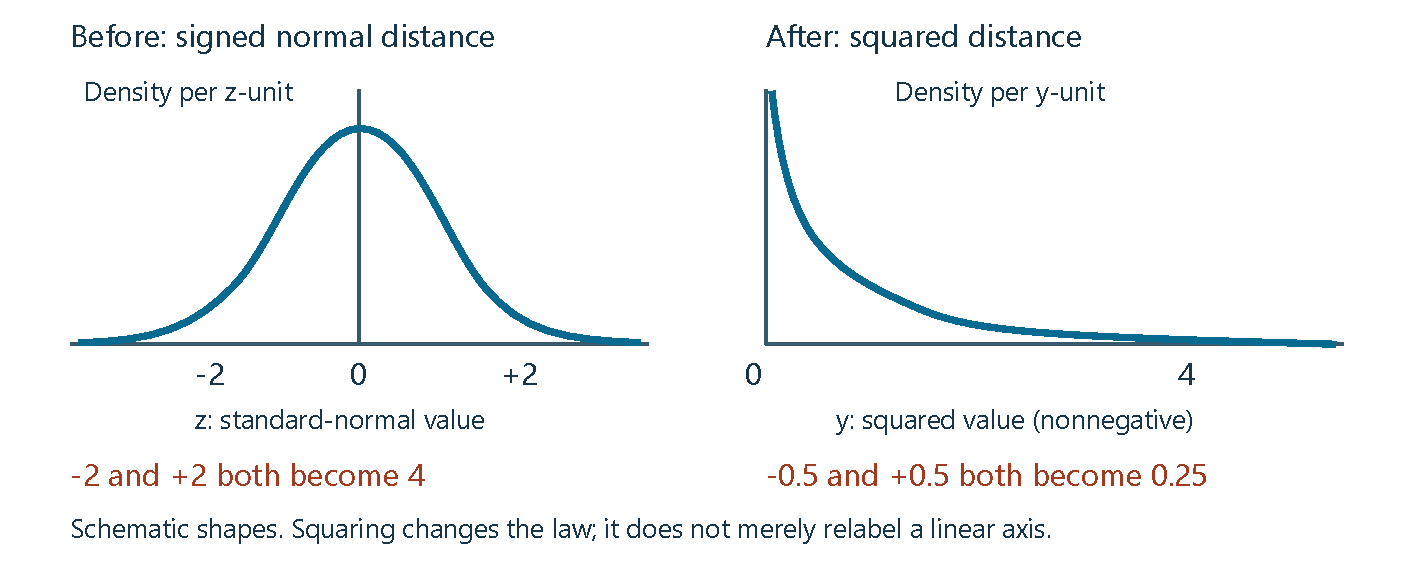
\includegraphics[width=\linewidth,height=.62\textheight,keepaspectratio]{asset-43c44d9700c380f0f903e025a65428d8a5d4e4500a5d7ac019cfae07076d7799.pdf}\end{center}

\medskip

Adding independent squared standard-Normal components gives a chi-square variable whose degrees of freedom count those independent components. The displayed density and gamma-function definition express this family mathematically. The construction matters because it explains the model's nonnegative range and its changing shape as the number of components increases.


Sample variance has a closely related structure. Centring the observations about a fitted mean imposes a zero-sum constraint on their residuals and removes one degree of freedom. The six-residual calculation in \hyperref[material-ab96dad68bbbb1e43e0e6b8543370bb77e63949d2c4e917575d9ed434971bb91]{Fig.~\ref*{material-ab96dad68bbbb1e43e0e6b8543370bb77e63949d2c4e917575d9ed434971bb91}} connects the nitrate sample to this construction. Under independent Normal sampling, an orthogonal representation supplies the remaining independent components that justify the chi-square reference for the scaled residual sum of squares.


\par\medskip
\Needspace{10cm}
\refstepcounter{figure}\label{material-ab96dad68bbbb1e43e0e6b8543370bb77e63949d2c4e917575d9ed434971bb91}
\noindent\textbf{Fig.~\ref*{material-ab96dad68bbbb1e43e0e6b8543370bb77e63949d2c4e917575d9ed434971bb91}.} The six nitrate residuals are divided by the independently known reference SD, squared and added. Their squared standardized values sum to 12; estimating the mean leaves five degrees of freedom.\par\nopagebreak
\begin{center}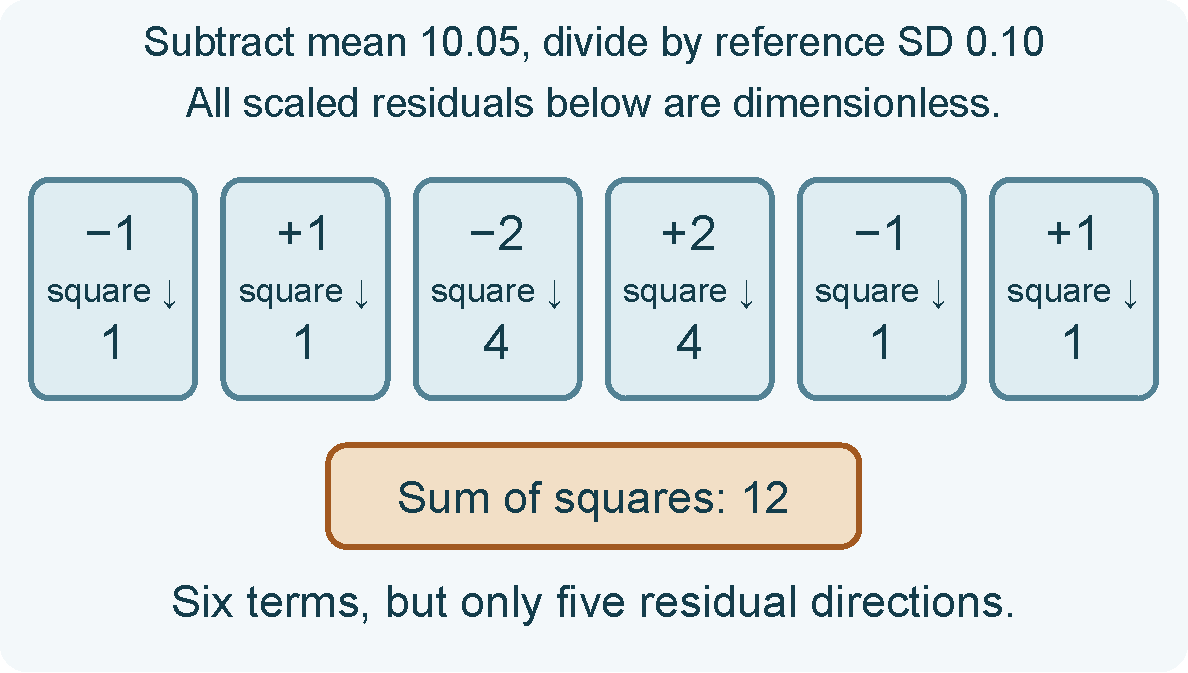
\includegraphics[width=\linewidth,height=.62\textheight,keepaspectratio]{asset-7c9ea0627c16f08ca64ad3732617c9f81589739cd127befcaa2a2543faa4abad.pdf}\end{center}

\medskip

This connection turns repeated-sampling variation into a precision question. A sample variance is compared with a fixed reference variance through the displayed scaled statistic. An upper-tail decision asks whether the observed spread is unusually large under that reference model (\hyperref[material-5bda1ade42df9737c1227c9420d578336e4d448b6e98eb516fca98196807bf3a]{Fig.~\ref*{material-5bda1ade42df9737c1227c9420d578336e4d448b6e98eb516fca98196807bf3a}}). The sample degrees of freedom and the chosen tail probability determine the cutoff.


\par\medskip
\Needspace{10cm}
\refstepcounter{figure}\label{material-5bda1ade42df9737c1227c9420d578336e4d448b6e98eb516fca98196807bf3a}
\noindent\textbf{Fig.~\ref*{material-5bda1ade42df9737c1227c9420d578336e4d448b6e98eb516fca98196807bf3a}.} The five-degree-of-freedom chi-square curve marks the upper 5\% cutoff at 11.07 and the observed statistic at 12. The shaded upper probability beyond 12 is about 3.48\%.\par\nopagebreak
\begin{center}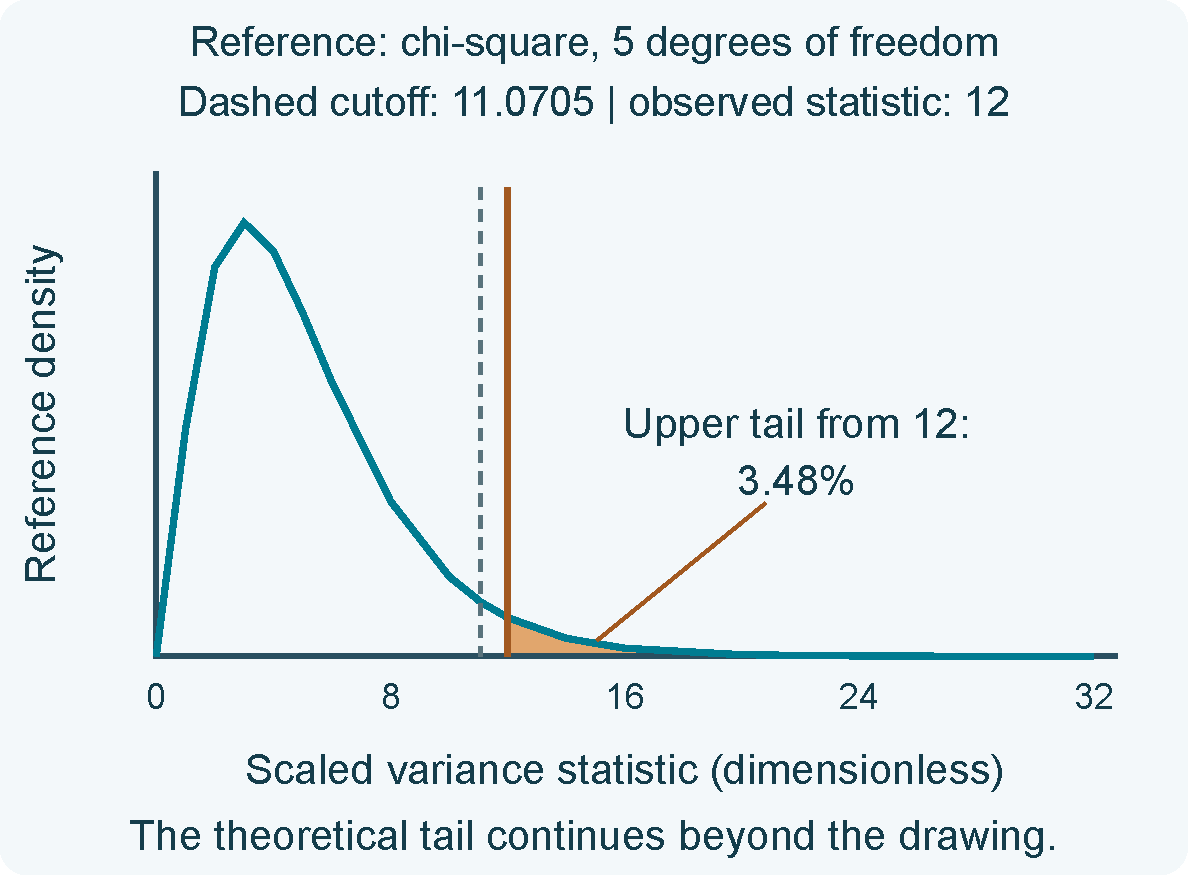
\includegraphics[width=\linewidth,height=.62\textheight,keepaspectratio]{asset-4d142e138ab9064cf02c870f20d8b938dd10d2a14aad360a2812e8e11fc4b00a.pdf}\end{center}

\medskip

The squared component in \hyperref[material-df8521cca903a7c6511ea2d5d10e8efe3e5efdbfc530494124be767014697f8a]{Eq.~\ref*{material-df8521cca903a7c6511ea2d5d10e8efe3e5efdbfc530494124be767014697f8a}} and the independent-component sum in \hyperref[material-c2bd9408dc2ec5e8c248ad1151d53e39092abf7c5e523ec67bf7c55f511d53f8]{Eq.~\ref*{material-c2bd9408dc2ec5e8c248ad1151d53e39092abf7c5e523ec67bf7c55f511d53f8}} explain the chi-square construction; the repeated sums in \hyperref[material-a6448e127e2412364da57f6efddc6edd0edbc8041cf04cbc543f5058a231a540]{Fig.~\ref*{material-a6448e127e2412364da57f6efddc6edd0edbc8041cf04cbc543f5058a231a540}} show its shape. For the precision check, \hyperref[material-e8b121575764015b30363f613297591e7f5ccd438665ce632e78f008174fc250]{Eq.~\ref*{material-e8b121575764015b30363f613297591e7f5ccd438665ce632e78f008174fc250}} scales the observed sample spread, and \hyperref[material-aca2b3146a57bf8d0dacdc7ecf148adfa52d7ace1b716b17d716afba0f642ecb]{Eq.~\ref*{material-aca2b3146a57bf8d0dacdc7ecf148adfa52d7ace1b716b17d716afba0f642ecb}} compares it with the upper-tail cutoff. The calculation quantifies compatibility with the stated reference variance under the sampling assumptions. An unusually large value provides a reason to investigate the method's precision using the measurement conditions and analytical records.


\par\medskip
\noindent\begin{minipage}{\linewidth}
\refstepcounter{equation}\label{material-df8521cca903a7c6511ea2d5d10e8efe3e5efdbfc530494124be767014697f8a}
\noindent\textbf{Eq.~\ref*{material-df8521cca903a7c6511ea2d5d10e8efe3e5efdbfc530494124be767014697f8a}.} A squared standard-Normal component follows a one-degree-of-freedom chi-square distribution.\par\nopagebreak
\begin{center}\begin{adjustbox}{max width=\linewidth}$\displaystyle \begin{gathered}Z\sim\mathcal N(0,1),\quad Y=Z^2\sim\chi^2_1\\(-2)^2=(+2)^2=4\\(-0.5)^2=(+0.5)^2=0.25\end{gathered}$\end{adjustbox}\end{center}

\par\noindent\textbf{Symbols}

\begin{itemize}\setlength{\itemsep}{1pt}\setlength{\parsep}{0pt}
\item \textbf{Z}: Standard-normal random variable; mean zero and variance one.
\item \textbf{Y}: Square of Z; a nonnegative random variable.
\item \textbf{N(0, 1)}: Normal distribution with mean zero and variance one.
\item \textbf{\ensuremath{\chi}\ensuremath{{}^2}\ensuremath{{}_1}}: Chi-square distribution with one degree of freedom.
\item \textbf{\ensuremath{\sim}}: Follows the named distribution.
\item \textbf{\ensuremath{{}^2}, =}: Squaring; equality evaluating or defining a value.
\item \textbf{+, \ensuremath{-}}: Signs indicating direction before squaring.
\end{itemize}

All quantities are dimensionless. Parentheses group signed values; squaring folds both tails onto the nonnegative axis.

\end{minipage}\par
\medskip

\par\medskip
\noindent\begin{minipage}{\linewidth}
\refstepcounter{equation}\label{material-c2bd9408dc2ec5e8c248ad1151d53e39092abf7c5e523ec67bf7c55f511d53f8}
\noindent\textbf{Eq.~\ref*{material-c2bd9408dc2ec5e8c248ad1151d53e39092abf7c5e523ec67bf7c55f511d53f8}.} Independent squared Normal components, chi-square density and gamma-function normalization.\par\nopagebreak
\begin{center}\begin{adjustbox}{max width=\linewidth}$\displaystyle \begin{gathered}X=\sum_{i=1}^{k}Z_i^2\sim\chi^2_k\\f_k(x)=\frac{x^{k/2-1}e^{-x/2}}{2^{k/2}\Gamma(k/2)},\quad x>0,\;k>0\\\Gamma(a)=\int_0^\infty t^{a-1}e^{-t}\,dt,\quad a>0\end{gathered}$\end{adjustbox}\end{center}

\par\noindent\textbf{Symbols}

\begin{itemize}\setlength{\itemsep}{1pt}\setlength{\parsep}{0pt}
\item \textbf{\ensuremath{\Gamma}(a)}: Gamma function at positive real argument a.
\item \textbf{a}: Dimensionless argument; here k/2.
\item \textbf{t}: Dimensionless integration variable.
\item \textbf{\ensuremath{\int}\ensuremath{{}_0}\ensuremath{\infty}}: Integral over t from zero to positive infinity.
\item \textbf{dt}: Infinitesimal increment of t.
\item \textbf{t\ensuremath{{}^a}\ensuremath{{}^-}\ensuremath{{}^1}, e\ensuremath{{}^-}\ensuremath{{}^t}}: A power of t and the natural exponential with exponent \ensuremath{-}t.
\end{itemize}

All quantities are dimensionless. For a positive integer m, \ensuremath{\Gamma}(m) = (m \ensuremath{-} 1) factorial.

\begin{itemize}\setlength{\itemsep}{1pt}\setlength{\parsep}{0pt}
\item \textbf{X}: Random chi-square variable (dimensionless).
\item \textbf{x}: Concrete value of X (dimensionless).
\item \textbf{f\ensuremath{{}_k}(x)}: Probability density at x for k degrees of freedom.
\item \textbf{k}: Degrees of freedom; a positive real parameter of the density family.
\item \textbf{e}: Base of the natural exponential.
\item \textbf{\ensuremath{\Gamma}(k/2)}: Gamma function evaluated at k/2; part of the density normalization.
\item \textbf{Powers}: Superscripts raise their bases to the stated exponents.
\item \textbf{Multiplication, /, \ensuremath{-}}: Adjacent factors multiply; fractions divide; minus subtracts or negates.
\item \textbf{>, =}: Greater than; equality defining the density.
\end{itemize}

Domain: x > 0. Density is zero for x < 0, and the probability of exactly zero is zero. The independent-square construction uses integer k. Parentheses group function arguments; total density area is one.

\begin{itemize}\setlength{\itemsep}{1pt}\setlength{\parsep}{0pt}
\item \textbf{Z\ensuremath{{}_i}}: Standard-normal component i, with mean zero and variance one.
\item \textbf{i}: Component index, from 1 through k.
\item \textbf{k}: Positive integer number of independent components.
\item \textbf{\ensuremath{\Sigma}, +}: Add the squared components.
\item \textbf{\ensuremath{{}^2}}: Square each component.
\item \textbf{\ensuremath{\chi}\ensuremath{{}^2}\ensuremath{{}_k}}: Chi-square distribution with k degrees of freedom.
\item \textbf{\ensuremath{\sim}}: Follows the stated distribution.
\end{itemize}

Condition: the Z\ensuremath{{}_i} are independent. All variables and their squared sum are dimensionless.

\end{minipage}\par
\medskip

\par\medskip
\noindent\begin{minipage}{\linewidth}
\refstepcounter{equation}\label{material-e8b121575764015b30363f613297591e7f5ccd438665ce632e78f008174fc250}
\noindent\textbf{Eq.~\ref*{material-e8b121575764015b30363f613297591e7f5ccd438665ce632e78f008174fc250}.} The sample residual sum of squares scaled by an independently known reference variance.\par\nopagebreak
\begin{center}\begin{adjustbox}{max width=\linewidth}$\displaystyle q=\sum_{i=1}^{6}\left(\frac{x_i-\bar x}{\sigma_0}\right)^2=\frac{0.12}{0.10^2}=12$\end{adjustbox}\end{center}

\par\noindent\textbf{Symbols}

\begin{itemize}\setlength{\itemsep}{1pt}\setlength{\parsep}{0pt}
\item \textbf{q}: Observed statistic for this series (dimensionless).
\item \textbf{x\ensuremath{{}_i}}: IC measurement result i (mg/L).
\item \textbf{\ensuremath{\bar{x}}}: Sample mean, 10.05 mg/L; the bar denotes averaging.
\item \textbf{\ensuremath{\sigma}\ensuremath{{}_0}}: Independently known reference SD, 0.10 mg/L; subscript 0 labels the reference.
\end{itemize}

\begin{itemize}\setlength{\itemsep}{1pt}\setlength{\parsep}{0pt}
\item \textbf{\ensuremath{\Sigma}}: Add all six indexed terms.
\item \textbf{i}: Measurement index, from 1 through 6.
\item \textbf{\ensuremath{-}}: Subtract the sample mean from a measurement.
\item \textbf{/, \ensuremath{{}^2}}: Divide by the reference SD, then square the ratio.
\item \textbf{=}: Rewrites the same calculation; parentheses group each ratio.
\end{itemize}

The squared-deviation sum is 0.12 (mg/L)\ensuremath{{}^2}. Dividing by (0.10 mg/L)\ensuremath{{}^2} cancels the units and gives q = 12.

\end{minipage}\par
\medskip

\par\medskip
\noindent\begin{minipage}{\linewidth}
\refstepcounter{equation}\label{material-aca2b3146a57bf8d0dacdc7ecf148adfa52d7ace1b716b17d716afba0f642ecb}
\noindent\textbf{Eq.~\ref*{material-aca2b3146a57bf8d0dacdc7ecf148adfa52d7ace1b716b17d716afba0f642ecb}.} An upper-tail chi-square precision decision with five degrees of freedom.\par\nopagebreak
\begin{center}\begin{adjustbox}{max width=\linewidth}$\displaystyle \begin{gathered}H_0:\sigma\le\sigma_0,\quad H_1:\sigma>\sigma_0\\q=12>\chi^2_{5;0.95}\approx11.07\\p=P_{\sigma=\sigma_0}(Q\ge12)\approx0.03479\end{gathered}$\end{adjustbox}\end{center}

\par\noindent\textbf{Symbols}

\begin{itemize}\setlength{\itemsep}{1pt}\setlength{\parsep}{0pt}
\item \textbf{:}: Introduces the statement of a hypothesis.
\item \textbf{\ensuremath{\le}, >, \ensuremath{\ge}}: At most, greater than and at least.
\item \textbf{=, \ensuremath{\approx}}: Equality and approximate equality.
\item \textbf{\ensuremath{\alpha}}: Prespecified significance level, 0.05.
\end{itemize}

For \ensuremath{\sigma} below \ensuremath{\sigma}\ensuremath{{}_0}, the upper-tail rejection probability is smaller. Calibration at \ensuremath{\sigma} = \ensuremath{\sigma}\ensuremath{{}_0} therefore controls the composite null.

\begin{itemize}\setlength{\itemsep}{1pt}\setlength{\parsep}{0pt}
\item \textbf{H\ensuremath{{}_0}}: True repeatability SD is at most the reference SD.
\item \textbf{H\ensuremath{{}_1}}: True repeatability SD exceeds the reference SD.
\item \textbf{\ensuremath{\sigma}}: True repeatability SD (mg/L).
\item \textbf{\ensuremath{\sigma}\ensuremath{{}_0}}: Known reference SD, 0.10 mg/L; subscript 0 identifies the reference.
\end{itemize}

The comparison concerns repeatability spread.

\begin{itemize}\setlength{\itemsep}{1pt}\setlength{\parsep}{0pt}
\item \textbf{q}: Observed QC statistic, 12.
\item \textbf{Q}: Random statistic under the boundary model.
\item \textbf{\ensuremath{\chi}\ensuremath{{}^2}\ensuremath{{}_5};\ensuremath{{}_0}.\ensuremath{{}_9}\ensuremath{{}_5}}: 95th percentile of chi-square with five degrees of freedom.
\item \textbf{P}: Probability under the null boundary \ensuremath{\sigma} = \ensuremath{\sigma}\ensuremath{{}_0}.
\item \textbf{p}: Upper-tail probability P(Q \ensuremath{\ge} q) under that boundary.
\end{itemize}

All these quantities are dimensionless. The p-value is a probability about the statistic under the stated model.

\end{minipage}\par
\medskip

\par\medskip
\Needspace{10cm}
\refstepcounter{figure}\label{material-a6448e127e2412364da57f6efddc6edd0edbc8041cf04cbc543f5058a231a540}
\noindent\textbf{Fig.~\ref*{material-a6448e127e2412364da57f6efddc6edd0edbc8041cf04cbc543f5058a231a540}.} The histogram contains 1,000 repeated sums of two independent squared standard-Normal components. Their simulated mean is 1.993, close to the theoretical mean of 2. The overlaid chi-square density has two degrees of freedom, matching the component count.\par\nopagebreak
\begin{center}
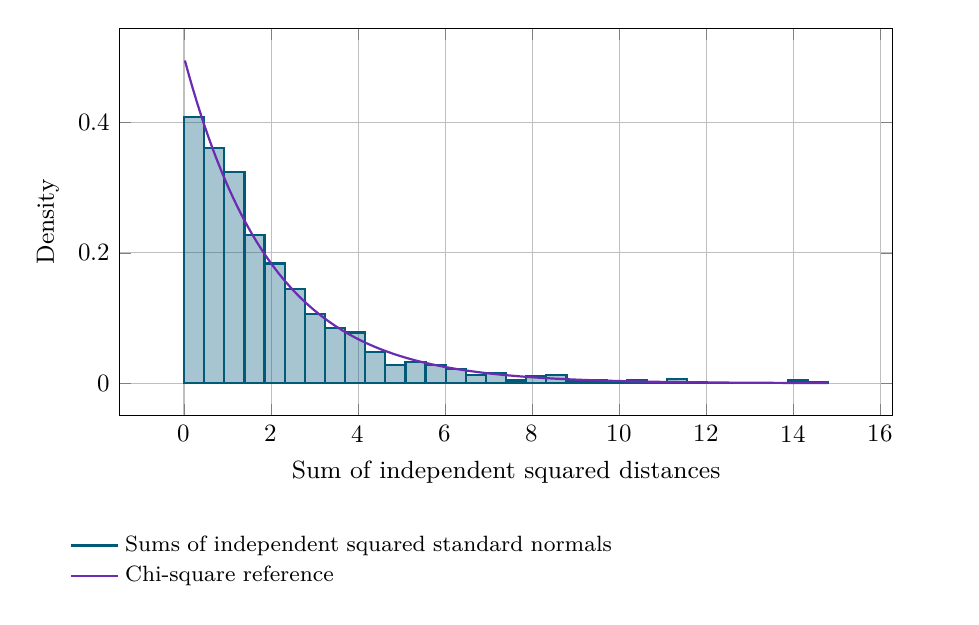
\begin{tikzpicture}
\begin{axis}[width=0.94\linewidth,
height=6.5cm,
scale only axis=false,
grid=major,
tick label style={font=\small},
label style={font=\small},
xlabel={Sum of independent squared distances},
ylabel={Density},
legend style={font=\footnotesize,draw=none,at={(0.5,-0.28)},anchor=north,legend columns=1,text width=0.85\linewidth,align=left},
unbounded coords=jump,
scaled ticks=false]
\addplot[color=pcd1,thick,fill=pcd1,fill opacity=0.35,mark=none] coordinates {(0.0004987396513015108,0) (0.0004987396513015108,0.40865501120384534) (0.4629915387564201,0.40865501120384534) (0.4629915387564201,0)} \closedcycle;
\addplot[color=pcd1,thick,fill=pcd1,fill opacity=0.35,forget plot,mark=none] coordinates {(0.46299153875642,0) (0.46299153875642,0.3610867030213872) (0.9254843378615385,0.3610867030213872) (0.9254843378615385,0)} \closedcycle;
\addplot[color=pcd1,thick,fill=pcd1,fill opacity=0.35,forget plot,mark=none] coordinates {(0.9254843378615385,0) (0.9254843378615385,0.3243293739713058) (1.3879771369666571,0.3243293739713058) (1.3879771369666571,0)} \closedcycle;
\addplot[color=pcd1,thick,fill=pcd1,fill opacity=0.35,forget plot,mark=none] coordinates {(1.387977136966657,0) (1.387977136966657,0.22703056177991407) (1.8504699360717756,0.22703056177991407) (1.8504699360717756,0)} \closedcycle;
\addplot[color=pcd1,thick,fill=pcd1,fill opacity=0.35,forget plot,mark=none] coordinates {(1.8504699360717753,0) (1.8504699360717753,0.18378664525040664) (2.3129627351768938,0.18378664525040664) (2.3129627351768938,0)} \closedcycle;
\addplot[color=pcd1,thick,fill=pcd1,fill opacity=0.35,forget plot,mark=none] coordinates {(2.312962735176894,0) (2.312962735176894,0.14486712037384994) (2.7754555342820124,0.14486712037384994) (2.7754555342820124,0)} \closedcycle;
\addplot[color=pcd1,thick,fill=pcd1,fill opacity=0.35,forget plot,mark=none] coordinates {(2.775455534282013,0) (2.775455534282013,0.10594759549729324) (3.237948333387131,0.10594759549729324) (3.237948333387131,0)} \closedcycle;
\addplot[color=pcd1,thick,fill=pcd1,fill opacity=0.35,forget plot,mark=none] coordinates {(3.2379483333871315,0) (3.2379483333871315,0.08432563723253951) (3.7004411324922497,0.08432563723253951) (3.7004411324922497,0)} \closedcycle;
\addplot[color=pcd1,thick,fill=pcd1,fill opacity=0.35,forget plot,mark=none] coordinates {(3.7004411324922497,0) (3.7004411324922497,0.07783904975311338) (4.162933931597368,0.07783904975311338) (4.162933931597368,0)} \closedcycle;
\addplot[color=pcd1,thick,fill=pcd1,fill opacity=0.35,forget plot,mark=none] coordinates {(4.162933931597368,0) (4.162933931597368,0.047568308182458184) (4.625426730702487,0.047568308182458184) (4.625426730702487,0)} \closedcycle;
\addplot[color=pcd1,thick,fill=pcd1,fill opacity=0.35,forget plot,mark=none] coordinates {(4.625426730702486,0) (4.625426730702486,0.028108545744179834) (5.087919529807605,0.028108545744179834) (5.087919529807605,0)} \closedcycle;
\addplot[color=pcd1,thick,fill=pcd1,fill opacity=0.35,forget plot,mark=none] coordinates {(5.087919529807605,0) (5.087919529807605,0.03243293739713058) (5.550412328912724,0.03243293739713058) (5.550412328912724,0)} \closedcycle;
\addplot[color=pcd1,thick,fill=pcd1,fill opacity=0.35,forget plot,mark=none] coordinates {(5.550412328912723,0) (5.550412328912723,0.028108545744179834) (6.0129051280178425,0.028108545744179834) (6.0129051280178425,0)} \closedcycle;
\addplot[color=pcd1,thick,fill=pcd1,fill opacity=0.35,forget plot,mark=none] coordinates {(6.0129051280178425,0) (6.0129051280178425,0.021621958264753723) (6.475397927122962,0.021621958264753723) (6.475397927122962,0)} \closedcycle;
\addplot[color=pcd1,thick,fill=pcd1,fill opacity=0.35,forget plot,mark=none] coordinates {(6.475397927122961,0) (6.475397927122961,0.012973174958852232) (6.93789072622808,0.012973174958852232) (6.93789072622808,0)} \closedcycle;
\addplot[color=pcd1,thick,fill=pcd1,fill opacity=0.35,forget plot,mark=none] coordinates {(6.937890726228079,0) (6.937890726228079,0.015135370785327605) (7.400383525333198,0.015135370785327605) (7.400383525333198,0)} \closedcycle;
\addplot[color=pcd1,thick,fill=pcd1,fill opacity=0.35,forget plot,mark=none] coordinates {(7.400383525333198,0) (7.400383525333198,0.004324391652950744) (7.862876324438317,0.004324391652950744) (7.862876324438317,0)} \closedcycle;
\addplot[color=pcd1,thick,fill=pcd1,fill opacity=0.35,forget plot,mark=none] coordinates {(7.862876324438317,0) (7.862876324438317,0.010810979132376861) (8.325369123543435,0.010810979132376861) (8.325369123543435,0)} \closedcycle;
\addplot[color=pcd1,thick,fill=pcd1,fill opacity=0.35,forget plot,mark=none] coordinates {(8.325369123543437,0) (8.325369123543437,0.012973174958852232) (8.787861922648554,0.012973174958852232) (8.787861922648554,0)} \closedcycle;
\addplot[color=pcd1,thick,fill=pcd1,fill opacity=0.35,forget plot,mark=none] coordinates {(8.787861922648554,0) (8.787861922648554,0.004324391652950744) (9.250354721753672,0.004324391652950744) (9.250354721753672,0)} \closedcycle;
\addplot[color=pcd1,thick,fill=pcd1,fill opacity=0.35,forget plot,mark=none] coordinates {(9.250354721753673,0) (9.250354721753673,0.004324391652950744) (9.71284752085879,0.004324391652950744) (9.71284752085879,0)} \closedcycle;
\addplot[color=pcd1,thick,fill=pcd1,fill opacity=0.35,forget plot,mark=none] coordinates {(9.712847520858793,0) (9.712847520858793,0.002162195826475372) (10.17534031996391,0.002162195826475372) (10.17534031996391,0)} \closedcycle;
\addplot[color=pcd1,thick,fill=pcd1,fill opacity=0.35,forget plot,mark=none] coordinates {(10.17534031996391,0) (10.17534031996391,0.004324391652950744) (10.637833119069027,0.004324391652950744) (10.637833119069027,0)} \closedcycle;
\addplot[color=pcd1,thick,fill=pcd1,fill opacity=0.35,forget plot,mark=none] coordinates {(10.637833119069029,0) (10.637833119069029,0) (11.100325918174146,0) (11.100325918174146,0)} \closedcycle;
\addplot[color=pcd1,thick,fill=pcd1,fill opacity=0.35,forget plot,mark=none] coordinates {(11.100325918174148,0) (11.100325918174148,0.006486587479426116) (11.562818717279265,0.006486587479426116) (11.562818717279265,0)} \closedcycle;
\addplot[color=pcd1,thick,fill=pcd1,fill opacity=0.35,forget plot,mark=none] coordinates {(11.562818717279267,0) (11.562818717279267,0.002162195826475372) (12.025311516384384,0.002162195826475372) (12.025311516384384,0)} \closedcycle;
\addplot[color=pcd1,thick,fill=pcd1,fill opacity=0.35,forget plot,mark=none] coordinates {(12.025311516384384,0) (12.025311516384384,0) (12.487804315489502,0) (12.487804315489502,0)} \closedcycle;
\addplot[color=pcd1,thick,fill=pcd1,fill opacity=0.35,forget plot,mark=none] coordinates {(12.487804315489504,0) (12.487804315489504,0) (12.95029711459462,0) (12.95029711459462,0)} \closedcycle;
\addplot[color=pcd1,thick,fill=pcd1,fill opacity=0.35,forget plot,mark=none] coordinates {(12.950297114594623,0) (12.950297114594623,0) (13.41278991369974,0) (13.41278991369974,0)} \closedcycle;
\addplot[color=pcd1,thick,fill=pcd1,fill opacity=0.35,forget plot,mark=none] coordinates {(13.41278991369974,0) (13.41278991369974,0) (13.875282712804857,0) (13.875282712804857,0)} \closedcycle;
\addplot[color=pcd1,thick,fill=pcd1,fill opacity=0.35,forget plot,mark=none] coordinates {(13.875282712804859,0) (13.875282712804859,0.004324391652950744) (14.337775511909976,0.004324391652950744) (14.337775511909976,0)} \closedcycle;
\addplot[color=pcd1,thick,fill=pcd1,fill opacity=0.35,forget plot,mark=none] coordinates {(14.337775511909978,0) (14.337775511909978,0.002162195826475372) (14.800268311015095,0.002162195826475372) (14.800268311015095,0)} \closedcycle;
\addlegendentry{Sums of independent squared standard normals}
\addplot[color=pcd2,thick,mark=none] coordinates {(0.02,0.4950249168745845) (0.11237667694384436,0.4726805356315686) (0.2047533538876887,0.45134473265625985) (0.2971300308315331,0.43097198285172095) (0.38950670777537744,0.4115188160279243) (0.48188338471922176,0.39294372414758555) (0.5742600616630662,0.3752070727587251) (0.6666367386069105,0.35827101642497694) (0.7590134155507549,0.3420994179731951) (0.8513900924945992,0.3266577713860526) (0.9437667694384435,0.31191312817510675) (1.0361434463822878,0.29783402707722806) (1.1285201233261324,0.2843904269243849) (1.2208968002699765,0.2715536425435445) (1.313273477213821,0.2592962835499165) (1.4056501541576651,0.2475921959029419) (1.4980268311015097,0.23641640610031978) (1.590403508045354,0.22574506789099982) (1.6827801849891983,0.21555541139343615) (1.7751568619330425,0.2058256945105377) (1.867533538876887,0.19653515653764375) (1.9599102158207313,0.1876639738645391) (2.0522868927645757,0.17919321767698537) (2.14466356970842,0.1711048135675177) (2.2370402466522648,0.16338150296932327) (2.3294169235961086,0.1560068063309147) (2.421793600539953,0.14896498795301988) (2.5141702774837973,0.1422410224126614) (2.606546954427642,0.13582056250278152) (2.6989236313714864,0.12968990861900556) (2.7913003083153303,0.12383597952822181) (2.8836769852591746,0.11824628445660601) (2.9760536622030194,0.11290889643753402) (3.0684303391468637,0.10781242686251331) (3.160807016090708,0.10294600118083176) (3.2531836930345523,0.09829923569607282) (3.3455603699783967,0.09386221540998774) (3.4379370469222414,0.08962547286644784) (3.530313723866085,0.08557996795033702) (3.622690400809929,0.08171706859827901) (3.715067077753774,0.07802853238004206) (3.8074437546976183,0.07450648891132028) (3.8998204316414626,0.07114342306036464) (3.992197108585307,0.06793215891263144) (4.084573785529151,0.06486584445923285) (4.176950462472996,0.06193793697651824) (4.2693271394168395,0.05914218906559068) (4.361703816360684,0.056472635321969944) (4.454080493304529,0.05392357960695914) (4.546457170248372,0.051489582893554806) (4.638833847192217,0.04916545166096688) (4.731210524136062,0.04694622681298606) (4.8235872010799055,0.044827173096552195) (4.91596387802375,0.0428037689979464) (5.008340554967594,0.04087169709504781) (5.100717231911439,0.039026834845069) (5.193093908855284,0.037265245788113764) (5.2854705857991275,0.03558317114778761) (5.377847262742972,0.033977021810939) (5.470223939686816,0.032443370669418325) (5.56260061663066,0.03097894530751352) (5.654977293574505,0.02958062101945956) (5.747353970518349,0.028245414142122865) (5.8397306474621935,0.026970475688634137) (5.932107324406038,0.025753085269385776) (6.024484001349882,0.024590645287422528) (6.116860678293727,0.02348067539583998) (6.209237355237571,0.022420807205364483) (6.301614032181416,0.021408779230821642) (6.39399070912526,0.020442432065710683) (6.486367386069104,0.019519703774588292) (6.578744063012949,0.018638625493430497) (6.671120739956793,0.017797317228585078) (6.763497416900638,0.016993983845350245) (6.855874093844482,0.016226911237620555) (6.948250770788325,0.01549446267042686) (7.040627447732169,0.014795075287566281) (7.133004124676014,0.014127256776870465) (7.225380801619858,0.01348958218599659) (7.317757478563703,0.012880690881946799) (7.4101341555075475,0.012299283647828568) (7.502510832451391,0.011744119910661183) (7.594887509395236,0.011214015094313136) (7.68726418633908,0.010707838091922463) (7.779640863282925,0.010224508852406585) (7.87201754022677,0.009762996075912052) (7.9643942171706135,0.00932231501328685) (8.056770894114457,0.008901525364879826) (8.149147571058302,0.008499729274183965) (8.241524248002147,0.008116069412042303) (8.333900924945992,0.00774972714732879) (8.426277601889836,0.00739992080020074) (8.51865427883368,0.007065903974195803) (8.611030955777524,0.006746963963614532) (8.703407632721369,0.006442420232790397) (8.795784309665214,0.00615162296400229) (8.888160986609059,0.005873951670931232) (8.980537663552902,0.005608813874702708) (9.072914340496745,0.005355643839689653) (9.16529101744059,0.00511390136637865) (9.257667694384434,0.004883070638723593) (9.350044371328279,0.004662659123527357) (9.442421048272124,0.004452196519503089) (9.534797725215967,0.004251233753772636) (9.627174402159811,0.0040593420236609175) (9.719551079103656,0.003876111881741707) (9.811927756047501,0.003701152362182485) (9.904304432991346,0.0035340901465242642) (9.996681109935189,0.003374568767116348) (10.089057786879033,0.0032222478465063547) (10.181434463822878,0.0030768023711626024) (10.273811140766723,0.0029379219979791035) (10.366187817710568,0.002805310392083476) (10.45856449465441,0.002678684594534809) (10.550941171598256,0.0025577744185623064) (10.6433178485421,0.002442321873056462) (10.735694525485945,0.00233208061208261) (10.82807120242979,0.0022268154092422816) (10.920447879373633,0.002126301655760783) (11.012824556317476,0.002030324881230035) (11.10520123326132,0.0019386802959840794) (11.197577910205165,0.0018511723541307884) (11.28995458714901,0.0017676143363073962) (11.382331264092855,0.0016878279512695707) (11.474707941036698,0.0016116429554639152) (11.567084617980543,0.0015388967897721581) (11.659461294924387,0.0014694342326519593) (11.751837971868232,0.0014031070689341932) (11.844214648812077,0.0013397737735700343) (11.93659132575592,0.0012792992096530287) (12.028968002699765,0.0012215543400718103) (12.12134467964361,0.0011664159521782155) (12.213721356587454,0.0011137663948832873) (12.306098033531299,0.0010634933276202172) (12.398474710475142,0.0010154894806385715) (12.490851387418987,0.0009696524261183255) (12.583228064362832,0.0009258843596153368) (12.675604741306676,0.0008840918913719005) (12.767981418250521,0.0008441858470471101) (12.860358095194364,0.0008060810774418307) (12.952734772138209,0.0007696962768122806) (13.045111449082052,0.0007349538093845642) (13.137488126025898,0.0007017795436999614) (13.229864802969741,0.0006701026944375348) (13.322241479913586,0.0006398556713765158) (13.41461815685743,0.0006109739351762252) (13.506994833801276,0.0005833958596657711) (13.599371510745119,0.0005570626003497124) (13.691748187688965,0.0005319179688490852) (13.784124864632808,0.0005079083130099113) (13.876501541576651,0.00048498240242334255) (13.968878218520496,0.0004630913191131939) (14.061254895464339,0.0004421883531576079) (14.153631572408186,0.00042222890302213447) (14.246008249352029,0.0004031703803915715) (14.338384926295873,0.0003849721192974872) (14.430761603239716,0.0003675952893475434) (14.523138280183563,0.00035100281287145645) (14.615514957127406,0.00033515928580682213) (14.707891634071252,0.000320030902155981) (14.800268311015095,0.00030558538185274515)};
\addlegendentry{Chi-square reference}

\end{axis}
\end{tikzpicture}
\end{center}

% Full-precision experiment details: {"blockId":"ex:rv-n36-v--block","parameters":[{"key":"df","label":"Independent squared components","value":2},{"key":"M","label":"Simulated complete series","value":1000},{"key":"seed","label":"Replay seed (Park-Miller)","value":20261102}],"readouts":[{"label":"Independent squared components","value":2},{"label":"Mean simulated sum","value":1.9929399091349982},{"label":"Theoretical mean","value":2}],"note":"Squaring produces nonnegative distances. Adding independent standard-Normal squares gives a chi-square variable. Its degrees of freedom count those components. The one-component density increases without bound towards zero.","markers":[[]]}

\medskip

\clearpage
\section{Estimating the standard error leads to Student's t}
A standardized mean would use the population standard deviation if that quantity were known. In practice, spread is often estimated from the same sample as the mean. The repeated experiment in \hyperref[material-0097b7b53e50628f182c206ec8c10194447bb7ab4ec1163b9c4512ff90ab65f7]{Fig.~\ref*{material-0097b7b53e50628f182c206ec8c10194447bb7ab4ec1163b9c4512ff90ab65f7}} shows what is estimated from each complete sample. The denominator then varies between complete repetitions as well as the numerator, so replacing a known standard deviation by a sample estimate changes the reference distribution.


\par\medskip
\Needspace{10cm}
\refstepcounter{figure}\label{material-0097b7b53e50628f182c206ec8c10194447bb7ab4ec1163b9c4512ff90ab65f7}
\noindent\textbf{Fig.~\ref*{material-0097b7b53e50628f182c206ec8c10194447bb7ab4ec1163b9c4512ff90ab65f7}.} One complete Normal sample supplies both its mean and estimated standard error. The process contributes one studentized value per repetition.\par\nopagebreak
\par\medskip\noindent\textcolor{pcd1}{\textbf{1. Take six measurements}}\par
Independent normally distributed results from one fixed population.

\par\noindent $\longrightarrow$ 2. estimate
\par\medskip\noindent\textcolor{pcd2}{\textbf{2. Estimate mean and SD}}\par
Both estimates change from sample to sample.

\par\noindent $\longrightarrow$ 3. center and scale
\par\medskip\noindent\textcolor{pcd3}{\textbf{3. Standardize the mean}}\par
Center at the true mean; divide by the estimated standard error.

\par\noindent $\longrightarrow$ 4. one value
\par\medskip\noindent\textcolor{pcd4}{\textbf{4. Collect, repeat, plot}}\par
One standardized value per complete sample. What distribution appears?


\medskip

Under independent, identically distributed Normal sampling, the mean is independent of the sample variance. Dividing the centred sample mean by its estimated standard error produces Student's t statistic with sample count minus one degrees of freedom. Each complete sample contributes one standardized mean to the resulting distribution.


The t distribution is symmetric and has heavier tails than the standard Normal for finite degrees of freedom. The additional tail probability reflects uncertainty introduced by estimating spread. The repeated-sample histogram in \hyperref[material-881d2574e16a98f164c772b71973a44d65531a24a45a629aa9a0ff07479f8360]{Fig.~\ref*{material-881d2574e16a98f164c772b71973a44d65531a24a45a629aa9a0ff07479f8360}} illustrates this distribution of standardized means.


\par\medskip
\Needspace{10cm}
\refstepcounter{figure}\label{material-881d2574e16a98f164c772b71973a44d65531a24a45a629aa9a0ff07479f8360}
\noindent\textbf{Fig.~\ref*{material-881d2574e16a98f164c772b71973a44d65531a24a45a629aa9a0ff07479f8360}.} Studentized means from 1,000 repeated two-result Normal samples form the histogram. The Student reference has one degree of freedom; the standard-Normal curve gives a known-spread comparison.\par\nopagebreak
\begin{center}
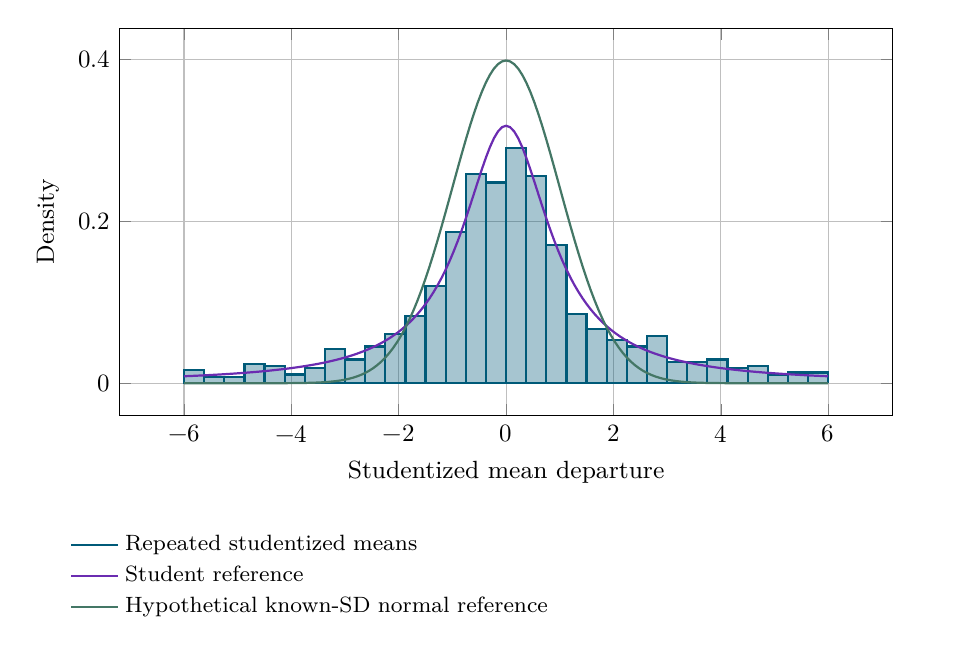
\begin{tikzpicture}
\begin{axis}[width=0.94\linewidth,
height=6.5cm,
scale only axis=false,
grid=major,
tick label style={font=\small},
label style={font=\small},
xlabel={Studentized mean departure},
ylabel={Density},
legend style={font=\footnotesize,draw=none,at={(0.5,-0.28)},anchor=north,legend columns=1,text width=0.85\linewidth,align=left},
unbounded coords=jump,
scaled ticks=false]
\addplot[color=pcd1,thick,fill=pcd1,fill opacity=0.35,mark=none] coordinates {(-6,0) (-6,0.016) (-5.625,0.016) (-5.625,0)} \closedcycle;
\addplot[color=pcd1,thick,fill=pcd1,fill opacity=0.35,forget plot,mark=none] coordinates {(-5.625,0) (-5.625,0.008) (-5.25,0.008) (-5.25,0)} \closedcycle;
\addplot[color=pcd1,thick,fill=pcd1,fill opacity=0.35,forget plot,mark=none] coordinates {(-5.25,0) (-5.25,0.008) (-4.875,0.008) (-4.875,0)} \closedcycle;
\addplot[color=pcd1,thick,fill=pcd1,fill opacity=0.35,forget plot,mark=none] coordinates {(-4.875,0) (-4.875,0.023999999999999997) (-4.5,0.023999999999999997) (-4.5,0)} \closedcycle;
\addplot[color=pcd1,thick,fill=pcd1,fill opacity=0.35,forget plot,mark=none] coordinates {(-4.5,0) (-4.5,0.021333333333333333) (-4.125,0.021333333333333333) (-4.125,0)} \closedcycle;
\addplot[color=pcd1,thick,fill=pcd1,fill opacity=0.35,forget plot,mark=none] coordinates {(-4.125,0) (-4.125,0.010666666666666666) (-3.75,0.010666666666666666) (-3.75,0)} \closedcycle;
\addplot[color=pcd1,thick,fill=pcd1,fill opacity=0.35,forget plot,mark=none] coordinates {(-3.75,0) (-3.75,0.018666666666666668) (-3.375,0.018666666666666668) (-3.375,0)} \closedcycle;
\addplot[color=pcd1,thick,fill=pcd1,fill opacity=0.35,forget plot,mark=none] coordinates {(-3.375,0) (-3.375,0.042666666666666665) (-3,0.042666666666666665) (-3,0)} \closedcycle;
\addplot[color=pcd1,thick,fill=pcd1,fill opacity=0.35,forget plot,mark=none] coordinates {(-3,0) (-3,0.029333333333333333) (-2.625,0.029333333333333333) (-2.625,0)} \closedcycle;
\addplot[color=pcd1,thick,fill=pcd1,fill opacity=0.35,forget plot,mark=none] coordinates {(-2.625,0) (-2.625,0.04533333333333334) (-2.25,0.04533333333333334) (-2.25,0)} \closedcycle;
\addplot[color=pcd1,thick,fill=pcd1,fill opacity=0.35,forget plot,mark=none] coordinates {(-2.25,0) (-2.25,0.06133333333333333) (-1.875,0.06133333333333333) (-1.875,0)} \closedcycle;
\addplot[color=pcd1,thick,fill=pcd1,fill opacity=0.35,forget plot,mark=none] coordinates {(-1.875,0) (-1.875,0.08266666666666667) (-1.5,0.08266666666666667) (-1.5,0)} \closedcycle;
\addplot[color=pcd1,thick,fill=pcd1,fill opacity=0.35,forget plot,mark=none] coordinates {(-1.5,0) (-1.5,0.12) (-1.125,0.12) (-1.125,0)} \closedcycle;
\addplot[color=pcd1,thick,fill=pcd1,fill opacity=0.35,forget plot,mark=none] coordinates {(-1.125,0) (-1.125,0.18666666666666668) (-0.75,0.18666666666666668) (-0.75,0)} \closedcycle;
\addplot[color=pcd1,thick,fill=pcd1,fill opacity=0.35,forget plot,mark=none] coordinates {(-0.75,0) (-0.75,0.25866666666666666) (-0.375,0.25866666666666666) (-0.375,0)} \closedcycle;
\addplot[color=pcd1,thick,fill=pcd1,fill opacity=0.35,forget plot,mark=none] coordinates {(-0.375,0) (-0.375,0.248) (0,0.248) (0,0)} \closedcycle;
\addplot[color=pcd1,thick,fill=pcd1,fill opacity=0.35,forget plot,mark=none] coordinates {(0,0) (0,0.2906666666666667) (0.375,0.2906666666666667) (0.375,0)} \closedcycle;
\addplot[color=pcd1,thick,fill=pcd1,fill opacity=0.35,forget plot,mark=none] coordinates {(0.375,0) (0.375,0.256) (0.75,0.256) (0.75,0)} \closedcycle;
\addplot[color=pcd1,thick,fill=pcd1,fill opacity=0.35,forget plot,mark=none] coordinates {(0.75,0) (0.75,0.17066666666666666) (1.125,0.17066666666666666) (1.125,0)} \closedcycle;
\addplot[color=pcd1,thick,fill=pcd1,fill opacity=0.35,forget plot,mark=none] coordinates {(1.125,0) (1.125,0.08533333333333333) (1.5,0.08533333333333333) (1.5,0)} \closedcycle;
\addplot[color=pcd1,thick,fill=pcd1,fill opacity=0.35,forget plot,mark=none] coordinates {(1.5,0) (1.5,0.06666666666666667) (1.875,0.06666666666666667) (1.875,0)} \closedcycle;
\addplot[color=pcd1,thick,fill=pcd1,fill opacity=0.35,forget plot,mark=none] coordinates {(1.875,0) (1.875,0.05333333333333334) (2.25,0.05333333333333334) (2.25,0)} \closedcycle;
\addplot[color=pcd1,thick,fill=pcd1,fill opacity=0.35,forget plot,mark=none] coordinates {(2.25,0) (2.25,0.04533333333333334) (2.625,0.04533333333333334) (2.625,0)} \closedcycle;
\addplot[color=pcd1,thick,fill=pcd1,fill opacity=0.35,forget plot,mark=none] coordinates {(2.625,0) (2.625,0.058666666666666666) (3,0.058666666666666666) (3,0)} \closedcycle;
\addplot[color=pcd1,thick,fill=pcd1,fill opacity=0.35,forget plot,mark=none] coordinates {(3,0) (3,0.02666666666666667) (3.375,0.02666666666666667) (3.375,0)} \closedcycle;
\addplot[color=pcd1,thick,fill=pcd1,fill opacity=0.35,forget plot,mark=none] coordinates {(3.375,0) (3.375,0.02666666666666667) (3.75,0.02666666666666667) (3.75,0)} \closedcycle;
\addplot[color=pcd1,thick,fill=pcd1,fill opacity=0.35,forget plot,mark=none] coordinates {(3.75,0) (3.75,0.029333333333333333) (4.125,0.029333333333333333) (4.125,0)} \closedcycle;
\addplot[color=pcd1,thick,fill=pcd1,fill opacity=0.35,forget plot,mark=none] coordinates {(4.125,0) (4.125,0.018666666666666668) (4.5,0.018666666666666668) (4.5,0)} \closedcycle;
\addplot[color=pcd1,thick,fill=pcd1,fill opacity=0.35,forget plot,mark=none] coordinates {(4.5,0) (4.5,0.021333333333333333) (4.875,0.021333333333333333) (4.875,0)} \closedcycle;
\addplot[color=pcd1,thick,fill=pcd1,fill opacity=0.35,forget plot,mark=none] coordinates {(4.875,0) (4.875,0.010666666666666666) (5.25,0.010666666666666666) (5.25,0)} \closedcycle;
\addplot[color=pcd1,thick,fill=pcd1,fill opacity=0.35,forget plot,mark=none] coordinates {(5.25,0) (5.25,0.013333333333333334) (5.625,0.013333333333333334) (5.625,0)} \closedcycle;
\addplot[color=pcd1,thick,fill=pcd1,fill opacity=0.35,forget plot,mark=none] coordinates {(5.625,0) (5.625,0.013333333333333334) (6,0.013333333333333334) (6,0)} \closedcycle;
\addlegendentry{Repeated studentized means}
\addplot[color=pcd2,thick,mark=none] coordinates {(-6,0.008602969896859207) (-5.925,0.008816074674895969) (-5.85,0.009037117927000942) (-5.775,0.009266494748895848) (-5.7,0.009504624848724712) (-5.625,0.00975195438763169) (-5.55,0.01000895798078109) (-5.475,0.010276140874761707) (-5.4,0.010554041319091196) (-5.325,0.010843233151526854) (-5.25,0.011144328619126141) (-5.175,0.011457981459516865) (-5.1,0.011784890269670154) (-5.025,0.012125802192663633) (-4.95,0.012481516956525458) (-4.875,0.012852891303320244) (-4.8,0.013240843851239208) (-4.725,0.013646360437664188) (-4.65,0.01407049999707329) (-4.575,0.014514401034343096) (-4.5,0.014979288761590139) (-4.425,0.0154664829753125) (-4.35,0.01597740676038603) (-4.275,0.016513596118610446) (-4.2,0.01707671063217761) (-4.125,0.017668545286871295) (-4.05,0.018291043596252863) (-3.975,0.018946312186825822) (-3.9,0.01963663702552687) (-3.825,0.02036450149522432) (-3.75,0.021132606551620955) (-3.675,0.02194389322650976) (-3.6,0.022801567778208496) (-3.525,0.023709129830737162) (-3.45,0.02467040388946255) (-3.375,0.02568957467309281) (-3.3,0.026771226760621585) (-3.225,0.027920389117595795) (-3.15,0.029142585139280447) (-3.075,0.03044388892904925) (-3,0.031830988618379054) (-2.925,0.033311257629280194) (-2.85,0.03489283487901239) (-2.775,0.03658471502722972) (-2.7,0.03839684996185652) (-2.625,0.040340262803490304) (-2.55,0.04242717576591677) (-2.475,0.04467115322288088) (-2.4,0.0470872612697915) (-2.325,0.04969224489160552) (-2.25,0.0525047234942335) (-2.175,0.055545404939913307) (-2.1,0.05883731722436055) (-2.025,0.0624060553723888) (-1.9500000000000002,0.06628003876809799) (-1.875,0.07049077064277715) (-1.7999999999999998,0.07507308636410157) (-1.7249999999999996,0.08006536989373764) (-1.6500000000000004,0.08550970750404044) (-1.5750000000000002,0.09145193354176064) (-1.5,0.09794150344116635) (-1.4249999999999998,0.10503110288596931) (-1.3499999999999996,0.11277586755847324) (-1.2750000000000004,0.12123204424995589) (-1.2000000000000002,0.1304548713867994) (-1.125,0.14049539803974206) (-1.0499999999999998,0.1513959030600669) (-0.9749999999999996,0.16318353665301671) (-0.9000000000000004,0.17586181557115496) (-0.8250000000000002,0.1893997091461751) (-0.75,0.203718327157626) (-0.6749999999999998,0.21867574834438172) (-0.5999999999999996,0.23405138689984611) (-0.5250000000000004,0.24953249284373585) (-0.4500000000000002,0.2647067660572063) (-0.375,0.27906620158578904) (-0.2999999999999998,0.29202741851723907) (-0.22499999999999964,0.30297193212020523) (-0.15000000000000036,0.3113055121601864) (-0.07500000000000018,0.31652940826231507) (0,0.31830988618379064) (0.07500000000000018,0.31652940826231507) (0.15000000000000036,0.3113055121601864) (0.22499999999999964,0.30297193212020523) (0.2999999999999998,0.29202741851723907) (0.375,0.27906620158578904) (0.4500000000000002,0.2647067660572063) (0.5250000000000004,0.24953249284373585) (0.5999999999999996,0.23405138689984611) (0.6749999999999998,0.21867574834438172) (0.75,0.203718327157626) (0.8250000000000002,0.1893997091461751) (0.9000000000000004,0.17586181557115496) (0.9749999999999996,0.16318353665301671) (1.0499999999999998,0.1513959030600669) (1.125,0.14049539803974206) (1.2000000000000002,0.1304548713867994) (1.2750000000000004,0.12123204424995589) (1.3499999999999996,0.11277586755847324) (1.4249999999999998,0.10503110288596931) (1.5,0.09794150344116635) (1.5750000000000002,0.09145193354176064) (1.6500000000000004,0.08550970750404044) (1.7249999999999996,0.08006536989373764) (1.7999999999999998,0.07507308636410157) (1.875,0.07049077064277715) (1.9500000000000002,0.06628003876809799) (2.0250000000000004,0.062406055372388775) (2.0999999999999996,0.05883731722436058) (2.1750000000000007,0.05554540493991326) (2.25,0.0525047234942335) (2.3249999999999993,0.049692244891605536) (2.4000000000000004,0.0470872612697915) (2.4749999999999996,0.04467115322288088) (2.5500000000000007,0.04242717576591675) (2.625,0.040340262803490304) (2.6999999999999993,0.038396849961856536) (2.7750000000000004,0.03658471502722971) (2.8499999999999996,0.03489283487901241) (2.9250000000000007,0.03331125762928018) (3,0.031830988618379054) (3.0749999999999993,0.030443888929049263) (3.1500000000000004,0.029142585139280433) (3.2249999999999996,0.027920389117595805) (3.3000000000000007,0.026771226760621575) (3.375,0.02568957467309281) (3.4499999999999993,0.02467040388946256) (3.5250000000000004,0.023709129830737155) (3.5999999999999996,0.022801567778208506) (3.6750000000000007,0.02194389322650975) (3.75,0.021132606551620955) (3.8249999999999993,0.020364501495224327) (3.9000000000000004,0.01963663702552687) (3.9749999999999996,0.018946312186825832) (4.050000000000001,0.018291043596252863) (4.125,0.017668545286871295) (4.199999999999999,0.017076710632177625) (4.275,0.016513596118610446) (4.35,0.01597740676038603) (4.425000000000001,0.015466482975312485) (4.5,0.014979288761590139) (4.574999999999999,0.014514401034343096) (4.65,0.01407049999707329) (4.725,0.013646360437664188) (4.800000000000001,0.013240843851239208) (4.875,0.012852891303320244) (4.949999999999999,0.012481516956525458) (5.025,0.012125802192663633) (5.1,0.011784890269670154) (5.175000000000001,0.011457981459516854) (5.25,0.011144328619126141) (5.324999999999999,0.010843233151526854) (5.4,0.010554041319091196) (5.475,0.010276140874761707) (5.550000000000001,0.010008957980781082) (5.625,0.00975195438763169) (5.699999999999999,0.009504624848724712) (5.775,0.009266494748895848) (5.85,0.009037117927000942) (5.925000000000001,0.008816074674895962) (6,0.008602969896859207)};
\addlegendentry{Student reference}
\addplot[color=pcd3,thick,mark=none] coordinates {(-6,6.075882849823286e-9) (-5.925,9.50211878502602e-9) (-5.85,1.4777079586480055e-8) (-5.775,2.2851455280615133e-8) (-5.7,3.513955094820434e-8) (-5.625,5.37323265056915e-8) (-5.55,8.17019037854322e-8) (-5.475,1.2353380011215305e-7) (-5.4,1.8573618445552897e-7) (-5.325,2.776926158966028e-7) (-5.25,4.1284709886299984e-7) (-5.175,6.103391606622874e-7) (-5.1,8.972435162383338e-7) (-5.025,0.0000013116154228950403) (-4.95,0.000001906600903122811) (-4.875,0.000002755942597549972) (-4.8,0.000003961299091032075) (-4.725,0.000005661899999034858) (-4.65,0.000008047182456492294) (-4.575,0.000011373197886886657) (-4.5,0.000015983741106905478) (-4.425,0.000022337335692076035) (-4.35,0.000031041407057850266) (-4.275,0.000042895182550127204) (-4.2,0.000058943067756539855) (-4.125,0.00008054044855559414) (-4.05,0.00010943404343980055) (-3.975,0.0001478590602980736) (-3.9,0.00019865547139277272) (-3.825,0.0002654056803802283) (-3.75,0.00035259568236744546) (-3.675,0.00046580147533503707) (-3.6,0.0006119019301137719) (-3.525,0.000799318528090754) (-3.45,0.0010382812956614103) (-3.375,0.0013411188734903778) (-3.3,0.0017225689390536812) (-3.225,0.0022001031503271315) (-3.15,0.002794258414879447) (-3.075,0.003528963655313759) (-3,0.0044318484119380075) (-2.925,0.005534516702780502) (-2.85,0.006872766690613971) (-2.775,0.00848673406223872) (-2.7,0.010420934814422592) (-2.625,0.012724181596831433) (-2.55,0.015449347134395174) (-2.475,0.018652948792269905) (-2.4,0.0223945302948429) (-2.325,0.026735820172248227) (-2.25,0.03173965183566742) (-2.175,0.03746863735223381) (-2.1,0.0439835959804272) (-2.025,0.051341749200769456) (-1.9500000000000002,0.059594706068816054) (-1.875,0.0687862758266919) (-1.7999999999999998,0.07895015830089419) (-1.7249999999999996,0.09010757603129817) (-1.6500000000000004,0.10226492456397797) (-1.5750000000000002,0.11541152807834995) (-1.5,0.12951759566589174) (-1.4249999999999998,0.1445324783229329) (-1.3499999999999996,0.16038332734191968) (-1.2750000000000004,0.17697425071017964) (-1.2000000000000002,0.19418605498321292) (-1.125,0.21187664577569948) (-1.0499999999999998,0.2298821406842331) (-0.9749999999999996,0.24801872461073723) (-0.9000000000000004,0.26608524989875476) (-0.8250000000000002,0.28386655352488727) (-0.75,0.30113743215480443) (-0.6749999999999998,0.31766718471514827) (-0.5999999999999996,0.3332246028917997) (-0.5250000000000004,0.34758326429234804) (-0.4500000000000002,0.36052696246164795) (-0.375,0.37185509386976895) (-0.2999999999999998,0.38138781546052414) (-0.22499999999999964,0.3889707880367495) (-0.15000000000000036,0.3944793309078889) (-0.07500000000000018,0.3978218316074972) (0,0.3989422804014327) (0.07500000000000018,0.3978218316074972) (0.15000000000000036,0.3944793309078889) (0.22499999999999964,0.3889707880367495) (0.2999999999999998,0.38138781546052414) (0.375,0.37185509386976895) (0.4500000000000002,0.36052696246164795) (0.5250000000000004,0.34758326429234804) (0.5999999999999996,0.3332246028917997) (0.6749999999999998,0.31766718471514827) (0.75,0.30113743215480443) (0.8250000000000002,0.28386655352488727) (0.9000000000000004,0.26608524989875476) (0.9749999999999996,0.24801872461073723) (1.0499999999999998,0.2298821406842331) (1.125,0.21187664577569948) (1.2000000000000002,0.19418605498321292) (1.2750000000000004,0.17697425071017964) (1.3499999999999996,0.16038332734191968) (1.4249999999999998,0.1445324783229329) (1.5,0.12951759566589174) (1.5750000000000002,0.11541152807834995) (1.6500000000000004,0.10226492456397797) (1.7249999999999996,0.09010757603129817) (1.7999999999999998,0.07895015830089419) (1.875,0.0687862758266919) (1.9500000000000002,0.059594706068816054) (2.0250000000000004,0.05134174920076941) (2.0999999999999996,0.04398359598042723) (2.1750000000000007,0.03746863735223372) (2.25,0.03173965183566742) (2.3249999999999993,0.026735820172248275) (2.4000000000000004,0.022394530294842882) (2.4749999999999996,0.018652948792269922) (2.5500000000000007,0.015449347134395141) (2.625,0.012724181596831433) (2.6999999999999993,0.010420934814422614) (2.7750000000000004,0.00848673406223871) (2.8499999999999996,0.006872766690613978) (2.9250000000000007,0.005534516702780487) (3,0.0044318484119380075) (3.0749999999999993,0.003528963655313768) (3.1500000000000004,0.0027942584148794424) (3.2249999999999996,0.0022001031503271332) (3.3000000000000007,0.0017225689390536767) (3.375,0.0013411188734903778) (3.4499999999999993,0.001038281295661414) (3.5250000000000004,0.0007993185280907532) (3.5999999999999996,0.0006119019301137731) (3.6750000000000007,0.0004658014753350354) (3.75,0.00035259568236744546) (3.8249999999999993,0.00026540568038022923) (3.9000000000000004,0.00019865547139277237) (3.9749999999999996,0.00014785906029807385) (4.050000000000001,0.00010943404343980016) (4.125,0.00008054044855559414) (4.199999999999999,0.00005894306775654006) (4.275,0.000042895182550127204) (4.35,0.000031041407057850266) (4.425000000000001,0.000022337335692075953) (4.5,0.000015983741106905478) (4.574999999999999,0.000011373197886886718) (4.65,0.000008047182456492294) (4.725,0.000005661899999034858) (4.800000000000001,0.000003961299091032062) (4.875,0.000002755942597549972) (4.949999999999999,0.000001906600903122818) (5.025,0.0000013116154228950403) (5.1,8.972435162383338e-7) (5.175000000000001,6.103391606622841e-7) (5.25,4.1284709886299984e-7) (5.324999999999999,2.7769261589660423e-7) (5.4,1.8573618445552897e-7) (5.475,1.2353380011215305e-7) (5.550000000000001,8.170190378543175e-8) (5.625,5.37323265056915e-8) (5.699999999999999,3.5139550948204466e-8) (5.775,2.2851455280615133e-8) (5.85,1.4777079586480055e-8) (5.925000000000001,9.502118785025951e-9) (6,6.075882849823286e-9)};
\addlegendentry{Hypothetical known-SD normal reference}

\end{axis}
\end{tikzpicture}
\end{center}

% Full-precision experiment details: {"blockId":"ex:rv-student-v--block","parameters":[{"key":"n","label":"Measurements per complete series","value":2},{"key":"sigma","label":"True method SD (mg/L), assumed","value":0.1},{"key":"M","label":"Simulated complete series","value":1000},{"key":"seed","label":"Replay seed (Park-Miller)","value":20261102},{"key":"view","label":"Distribution construction and shape","value":4}],"readouts":[{"label":"Measurements per simulated series","value":2},{"label":"Degrees of freedom","value":1}],"note":"Independent identically distributed Normal results make the sample mean and sample variance independent. Dividing a standardized mean by its estimated SD factor produces the Student distribution. The true SD stays fixed; small estimated denominators produce heavier tails. Increasing degrees of freedom brings the reference closer to the standard Normal.","markers":[[]]}

\medskip

As the degrees of freedom increase, the estimated denominator becomes more stable and the t reference approaches the standard Normal (\hyperref[material-fe8c268438bf8e0b3b4bc09a2ca01bc662d92f4e1e5071c3572eef3c2c97ca2d]{Fig.~\ref*{material-fe8c268438bf8e0b3b4bc09a2ca01bc662d92f4e1e5071c3572eef3c2c97ca2d}}). The construction in \hyperref[material-2c571729775eaad95cb8bb539621182b1c9f5d764c10bfc3db061d1b663465ea]{Eq.~\ref*{material-2c571729775eaad95cb8bb539621182b1c9f5d764c10bfc3db061d1b663465ea}} identifies how the sample mean and estimated standard error enter the statistic. The sampling assumptions justify this reference.


\par\medskip
\noindent\begin{minipage}{\linewidth}
\refstepcounter{equation}\label{material-2c571729775eaad95cb8bb539621182b1c9f5d764c10bfc3db061d1b663465ea}
\noindent\textbf{Eq.~\ref*{material-2c571729775eaad95cb8bb539621182b1c9f5d764c10bfc3db061d1b663465ea}.} Studentizing a Normal sample mean using its estimated standard error.\par\nopagebreak
\begin{center}\begin{adjustbox}{max width=\linewidth}$\displaystyle T=\frac{\bar X-\mu}{S/\sqrt n},\qquad n=6$\end{adjustbox}\end{center}

\par\noindent\textbf{Symbols}

\begin{itemize}\setlength{\itemsep}{1pt}\setlength{\parsep}{0pt}
\item \textbf{T}: Random standardized sample mean (dimensionless).
\item \textbf{\ensuremath{\bar{X}}}: Random sample mean (mg/L); the bar denotes averaging.
\item \textbf{\ensuremath{\mu}}: Fixed true population mean (mg/L).
\item \textbf{S}: Positive random sample SD estimated from the same sample (mg/L).
\item \textbf{n}: Dimensionless sample count, six here.
\item \textbf{S / \ensuremath{\sqrt{\vphantom{x}}}n}: Estimated standard error of the mean (mg/L); the square root is positive.
\item \textbf{\ensuremath{-}, /, =}: Centre the mean, divide by its estimated standard error, and define T.
\item \textbf{Comma}: Separates the definition from the stated sample count.
\end{itemize}

Condition: independent, identically distributed Normal measurement results. Sample variance uses divisor n \ensuremath{-} 1. Across complete samples, both estimated mean and SD vary while the population stays fixed.

\end{minipage}\par
\medskip

\par\medskip
\Needspace{10cm}
\refstepcounter{figure}\label{material-fe8c268438bf8e0b3b4bc09a2ca01bc662d92f4e1e5071c3572eef3c2c97ca2d}
\noindent\textbf{Fig.~\ref*{material-fe8c268438bf8e0b3b4bc09a2ca01bc662d92f4e1e5071c3572eef3c2c97ca2d}.} Student densities for samples of 4 and 30 measurements, corresponding to 3 and 29 degrees of freedom, share a standardized axis with the standard-Normal reference. The 29-degree-of-freedom curve lies closer to the Normal curve.\par\nopagebreak
\begin{center}
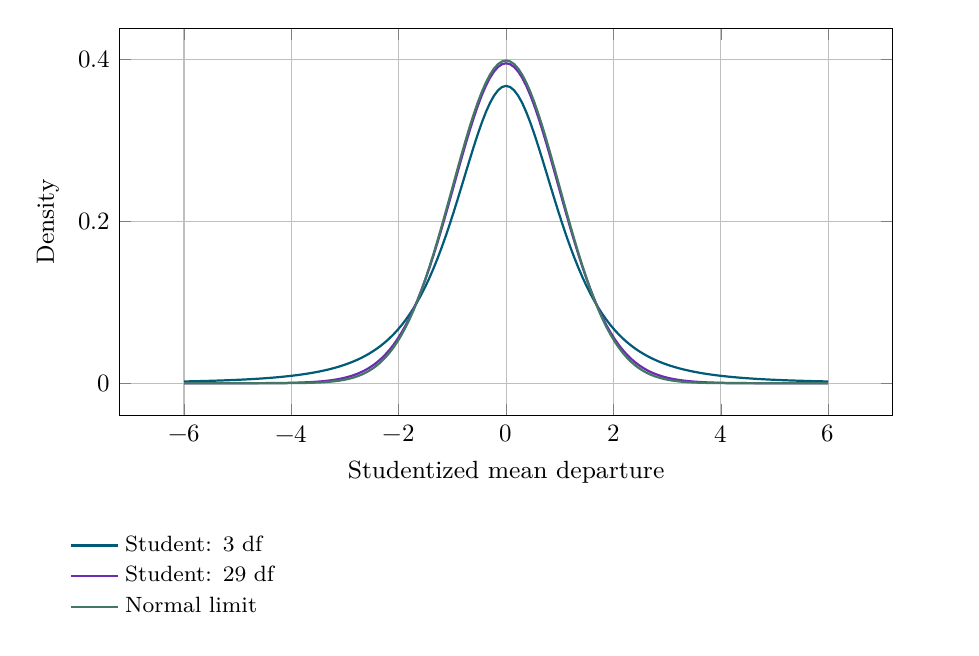
\begin{tikzpicture}
\begin{axis}[width=0.94\linewidth,
height=6.5cm,
scale only axis=false,
grid=major,
tick label style={font=\small},
label style={font=\small},
xlabel={Studentized mean departure},
ylabel={Density},
legend style={font=\footnotesize,draw=none,at={(0.5,-0.28)},anchor=north,legend columns=1,text width=0.85\linewidth,align=left},
unbounded coords=jump,
scaled ticks=false]
\addplot[color=pcd1,thick,mark=none] coordinates {(-6,0.0021748674375613093) (-5.925,0.0022781579246546626) (-5.85,0.002387541492787421) (-5.775,0.002503446071055316) (-5.7,0.002626334304505867) (-5.625,0.002756706731838621) (-5.55,0.002895105284866779) (-5.475,0.0030421171451263463) (-5.4,0.0031983789971654778) (-5.325,0.0033645817226986125) (-5.25,0.0035414755850296385) (-5.175,0.0037298759590040373) (-5.1,0.003930669668318859) (-5.025,0.004144821999385796) (-4.95,0.0043733844692001094) (-4.875,0.004617503433919167) (-4.8,0.004878429635210205) (-4.725,0.00515752879300815) (-4.65,0.005456293366259805) (-4.575,0.005776355617655806) (-4.5,0.006119502134407682) (-4.425,0.006487689974955604) (-4.35,0.006883064631232051) (-4.275,0.0073079800178844755) (-4.2,0.007765020723783577) (-4.125,0.008257026787282545) (-4.05,0.008787121285063745) (-3.975,0.009358741054946246) (-3.9,0.009975670905548968) (-3.825,0.010642081699863257) (-3.75,0.011362572735014191) (-3.675,0.012142218875902732) (-3.6,0.012986622934728544) (-3.525,0.013901973819753466) (-3.45,0.014895111002507185) (-3.375,0.015973595869435638) (-3.3,0.01714579052698204) (-3.225,0.018420944611900317) (-3.15,0.0198092906128036) (-3.075,0.021322148123501944) (-3,0.02297203730924133) (-2.925,0.024772801655057217) (-2.85,0.026739739757557012) (-2.775,0.02888974548781374) (-2.7,0.031241455256556472) (-2.625,0.0338154003076849) (-2.55,0.036634160896672055) (-2.475,0.03972251781026528) (-2.4,0.04310759487566397) (-2.325,0.046818983803563) (-2.25,0.05088883981538803) (-2.175,0.05535193292471191) (-2.1,0.060245635389509944) (-2.025,0.06560982066541379) (-1.9500000000000002,0.07148664316331484) (-1.875,0.07792016133214841) (-1.7999999999999998,0.08495575927973865) (-1.7249999999999996,0.09263931475881491) (-1.6500000000000004,0.10101605463646773) (-1.5750000000000002,0.11012903409971277) (-1.5,0.12001717451358736) (-1.4249999999999998,0.13071279933698934) (-1.3499999999999996,0.14223862075288085) (-1.2750000000000004,0.15460415517855958) (-1.2000000000000002,0.1678015873574969) (-1.125,0.18180116376022698) (-1.0499999999999998,0.19654627872710315) (-0.9749999999999996,0.21194852068050002) (-0.9000000000000004,0.22788306587380566) (-0.8250000000000002,0.24418493224669754) (-0.75,0.26064671694917585) (-0.6749999999999998,0.2770185109460898) (-0.5999999999999996,0.29301067996481295) (-0.5250000000000004,0.30830008960868877) (-0.4500000000000002,0.3225401088782245) (-0.375,0.3353743455331788) (-0.2999999999999998,0.3464535742745417) (-0.22499999999999964,0.35545477692493455) (-0.15000000000000036,0.3621007180122887) (-0.07500000000000018,0.3661781415719375) (0,0.36755259694786124) (0.07500000000000018,0.3661781415719375) (0.15000000000000036,0.3621007180122887) (0.22499999999999964,0.35545477692493455) (0.2999999999999998,0.3464535742745417) (0.375,0.3353743455331788) (0.4500000000000002,0.3225401088782245) (0.5250000000000004,0.30830008960868877) (0.5999999999999996,0.29301067996481295) (0.6749999999999998,0.2770185109460898) (0.75,0.26064671694917585) (0.8250000000000002,0.24418493224669754) (0.9000000000000004,0.22788306587380566) (0.9749999999999996,0.21194852068050002) (1.0499999999999998,0.19654627872710315) (1.125,0.18180116376022698) (1.2000000000000002,0.1678015873574969) (1.2750000000000004,0.15460415517855958) (1.3499999999999996,0.14223862075288085) (1.4249999999999998,0.13071279933698934) (1.5,0.12001717451358736) (1.5750000000000002,0.11012903409971277) (1.6500000000000004,0.10101605463646773) (1.7249999999999996,0.09263931475881491) (1.7999999999999998,0.08495575927973865) (1.875,0.07792016133214841) (1.9500000000000002,0.07148664316331484) (2.0250000000000004,0.06560982066541377) (2.0999999999999996,0.06024563538950997) (2.1750000000000007,0.05535193292471184) (2.25,0.05088883981538803) (2.3249999999999993,0.04681898380356303) (2.4000000000000004,0.04310759487566395) (2.4749999999999996,0.03972251781026529) (2.5500000000000007,0.03663416089667204) (2.625,0.0338154003076849) (2.6999999999999993,0.0312414552565565) (2.7750000000000004,0.028889745487813725) (2.8499999999999996,0.026739739757557012) (2.9250000000000007,0.024772801655057197) (3,0.02297203730924133) (3.0749999999999993,0.02132214812350196) (3.1500000000000004,0.019809290612803582) (3.2249999999999996,0.018420944611900317) (3.3000000000000007,0.01714579052698204) (3.375,0.015973595869435638) (3.4499999999999993,0.014895111002507198) (3.5250000000000004,0.013901973819753466) (3.5999999999999996,0.012986622934728544) (3.6750000000000007,0.012142218875902722) (3.75,0.011362572735014191) (3.8249999999999993,0.010642081699863257) (3.9000000000000004,0.009975670905548968) (3.9749999999999996,0.009358741054946254) (4.050000000000001,0.008787121285063745) (4.125,0.008257026787282545) (4.199999999999999,0.007765020723783577) (4.275,0.0073079800178844755) (4.35,0.006883064631232051) (4.425000000000001,0.006487689974955604) (4.5,0.006119502134407682) (4.574999999999999,0.005776355617655811) (4.65,0.005456293366259805) (4.725,0.00515752879300815) (4.800000000000001,0.0048784296352102005) (4.875,0.004617503433919167) (4.949999999999999,0.004373384469200113) (5.025,0.004144821999385796) (5.1,0.003930669668318859) (5.175000000000001,0.003729875959004034) (5.25,0.0035414755850296385) (5.324999999999999,0.0033645817226986155) (5.4,0.0031983789971654778) (5.475,0.0030421171451263463) (5.550000000000001,0.0028951052848667762) (5.625,0.002756706731838621) (5.699999999999999,0.0026263343045058694) (5.775,0.002503446071055316) (5.85,0.002387541492787421) (5.925000000000001,0.0022781579246546626) (6,0.0021748674375613093)};
\addlegendentry{Student: 3 df}
\addplot[color=pcd2,thick,mark=none] coordinates {(-6,0.0000021849248676871433) (-5.925,0.000002689643850038753) (-5.85,0.0000033117830630451967) (-5.775,0.000004078727485217324) (-5.7,0.000005024229412363959) (-5.625,0.000006189874245596557) (-5.55,0.000007626877329606368) (-5.475,0.000009398284256068167) (-5.4,0.000011581662085144383) (-5.325,0.000014272386837479284) (-5.25,0.000017587653830627192) (-5.175,0.00002167136248563757) (-5.1,0.00002670005666216833) (-5.025,0.00003289013597803565) (-4.95,0.0000405065935336168) (-4.875,0.00004987358158986161) (-4.8,0.0000613871595988529) (-4.725,0.00007553063903047828) (-4.65,0.0000928930070024059) (-4.575,0.00011419098589774699) (-4.5,0.00014029536870513698) (-4.425,0.00017226235903287901) (-4.35,0.0002113707392982254) (-4.275,0.000259165788320479) (-4.2,0.0003175109672511541) (-4.125,0.0003886484859494762) (-4.05,0.0004752699444590352) (-3.975,0.0005805983081661459) (-3.9,0.00070848251031951) (-3.825,0.0008635059691600608) (-3.75,0.0010511102434982663) (-3.675,0.0012777349118288143) (-3.6,0.0015509745247163497) (-3.525,0.0018797531242214934) (-3.45,0.002274516321316861) (-3.375,0.002747440244921732) (-3.3,0.003312655796629812) (-3.225,0.003986485537470492) (-3.15,0.004787689175474508) (-3.075,0.0057377120012457785) (-3,0.00686092873040413) (-2.925,0.008184873069846393) (-2.85,0.009740440963501181) (-2.775,0.011562052953232566) (-2.7,0.013687758504011688) (-2.625,0.01615926261786909) (-2.55,0.01902185276639495) (-2.475,0.022324202315203726) (-2.4,0.026118025442987976) (-2.325,0.03045755835233374) (-2.25,0.03539884263076079) (-2.175,0.040998789254823614) (-2.1,0.047314006226083304) (-2.025,0.05439937942734374) (-1.9500000000000002,0.062306405152476756) (-1.875,0.07108128393781118) (-1.7999999999999998,0.08076279869663723) (-1.7249999999999996,0.09138001543014074) (-1.6500000000000004,0.10294986144000907) (-1.5750000000000002,0.11547465324991965) (-1.5,0.12893966337578505) (-1.4249999999999998,0.1433108304846223) (-1.3499999999999996,0.1585327300127079) (-1.2750000000000004,0.17452693056359975) (-1.2000000000000002,0.1911908639922991) (-1.125,0.20839733277253827) (-1.0499999999999998,0.22599476609837071) (-0.9749999999999996,0.24380831567344846) (-0.9000000000000004,0.26164185332518136) (-0.8250000000000002,0.2792808961215668) (-0.75,0.2964964419296854) (-0.6749999999999998,0.31304965137715957) (-0.5999999999999996,0.3286972635990131) (-0.5250000000000004,0.343197586058745) (-0.4500000000000002,0.35631685644699007) (-0.375,0.3678357404824756) (-0.2999999999999998,0.3775557063545186) (-0.22499999999999964,0.38530500694142045) (-0.15000000000000036,0.3909440063483237) (-0.07500000000000018,0.3943696082179238) (0,0.3955185790117269) (0.07500000000000018,0.3943696082179238) (0.15000000000000036,0.3909440063483237) (0.22499999999999964,0.38530500694142045) (0.2999999999999998,0.3775557063545186) (0.375,0.3678357404824756) (0.4500000000000002,0.35631685644699007) (0.5250000000000004,0.343197586058745) (0.5999999999999996,0.3286972635990131) (0.6749999999999998,0.31304965137715957) (0.75,0.2964964419296854) (0.8250000000000002,0.2792808961215668) (0.9000000000000004,0.26164185332518136) (0.9749999999999996,0.24380831567344846) (1.0499999999999998,0.22599476609837071) (1.125,0.20839733277253827) (1.2000000000000002,0.1911908639922991) (1.2750000000000004,0.17452693056359975) (1.3499999999999996,0.1585327300127079) (1.4249999999999998,0.1433108304846223) (1.5,0.12893966337578505) (1.5750000000000002,0.11547465324991965) (1.6500000000000004,0.10294986144000907) (1.7249999999999996,0.09138001543014074) (1.7999999999999998,0.08076279869663723) (1.875,0.07108128393781118) (1.9500000000000002,0.062306405152476756) (2.0250000000000004,0.05439937942734374) (2.0999999999999996,0.047314006226083324) (2.1750000000000007,0.04099878925482352) (2.25,0.03539884263076079) (2.3249999999999993,0.03045755835233377) (2.4000000000000004,0.02611802544298795) (2.4749999999999996,0.022324202315203732) (2.5500000000000007,0.019021852766394915) (2.625,0.01615926261786909) (2.6999999999999993,0.013687758504011712) (2.7750000000000004,0.011562052953232545) (2.8499999999999996,0.009740440963501188) (2.9250000000000007,0.00818487306984637) (3,0.00686092873040413) (3.0749999999999993,0.005737712001245789) (3.1500000000000004,0.004787689175474499) (3.2249999999999996,0.003986485537470499) (3.3000000000000007,0.003312655796629806) (3.375,0.002747440244921732) (3.4499999999999993,0.002274516321316869) (3.5250000000000004,0.0018797531242214934) (3.5999999999999996,0.0015509745247163525) (3.6750000000000007,0.0012777349118288119) (3.75,0.0010511102434982663) (3.8249999999999993,0.0008635059691600623) (3.9000000000000004,0.0007084825103195088) (3.9749999999999996,0.0005805983081661459) (4.050000000000001,0.0004752699444590343) (4.125,0.0003886484859494762) (4.199999999999999,0.0003175109672511546) (4.275,0.000259165788320479) (4.35,0.0002113707392982254) (4.425000000000001,0.00017226235903287872) (4.5,0.00014029536870513698) (4.574999999999999,0.00011419098589774719) (4.65,0.0000928930070024059) (4.725,0.00007553063903047828) (4.800000000000001,0.0000613871595988528) (4.875,0.00004987358158986161) (4.949999999999999,0.000040506593533616876) (5.025,0.00003289013597803565) (5.1,0.00002670005666216833) (5.175000000000001,0.00002167136248563749) (5.25,0.000017587653830627192) (5.324999999999999,0.000014272386837479335) (5.4,0.000011581662085144383) (5.475,0.000009398284256068167) (5.550000000000001,0.000007626877329606341) (5.625,0.000006189874245596557) (5.699999999999999,0.000005024229412363968) (5.775,0.000004078727485217324) (5.85,0.0000033117830630451967) (5.925000000000001,0.0000026896438500387434) (6,0.0000021849248676871433)};
\addlegendentry{Student: 29 df}
\addplot[color=pcd3,thick,mark=none] coordinates {(-6,6.075882849823286e-9) (-5.925,9.50211878502602e-9) (-5.85,1.4777079586480055e-8) (-5.775,2.2851455280615133e-8) (-5.7,3.513955094820434e-8) (-5.625,5.37323265056915e-8) (-5.55,8.17019037854322e-8) (-5.475,1.2353380011215305e-7) (-5.4,1.8573618445552897e-7) (-5.325,2.776926158966028e-7) (-5.25,4.1284709886299984e-7) (-5.175,6.103391606622874e-7) (-5.1,8.972435162383338e-7) (-5.025,0.0000013116154228950403) (-4.95,0.000001906600903122811) (-4.875,0.000002755942597549972) (-4.8,0.000003961299091032075) (-4.725,0.000005661899999034858) (-4.65,0.000008047182456492294) (-4.575,0.000011373197886886657) (-4.5,0.000015983741106905478) (-4.425,0.000022337335692076035) (-4.35,0.000031041407057850266) (-4.275,0.000042895182550127204) (-4.2,0.000058943067756539855) (-4.125,0.00008054044855559414) (-4.05,0.00010943404343980055) (-3.975,0.0001478590602980736) (-3.9,0.00019865547139277272) (-3.825,0.0002654056803802283) (-3.75,0.00035259568236744546) (-3.675,0.00046580147533503707) (-3.6,0.0006119019301137719) (-3.525,0.000799318528090754) (-3.45,0.0010382812956614103) (-3.375,0.0013411188734903778) (-3.3,0.0017225689390536812) (-3.225,0.0022001031503271315) (-3.15,0.002794258414879447) (-3.075,0.003528963655313759) (-3,0.0044318484119380075) (-2.925,0.005534516702780502) (-2.85,0.006872766690613971) (-2.775,0.00848673406223872) (-2.7,0.010420934814422592) (-2.625,0.012724181596831433) (-2.55,0.015449347134395174) (-2.475,0.018652948792269905) (-2.4,0.0223945302948429) (-2.325,0.026735820172248227) (-2.25,0.03173965183566742) (-2.175,0.03746863735223381) (-2.1,0.0439835959804272) (-2.025,0.051341749200769456) (-1.9500000000000002,0.059594706068816054) (-1.875,0.0687862758266919) (-1.7999999999999998,0.07895015830089419) (-1.7249999999999996,0.09010757603129817) (-1.6500000000000004,0.10226492456397797) (-1.5750000000000002,0.11541152807834995) (-1.5,0.12951759566589174) (-1.4249999999999998,0.1445324783229329) (-1.3499999999999996,0.16038332734191968) (-1.2750000000000004,0.17697425071017964) (-1.2000000000000002,0.19418605498321292) (-1.125,0.21187664577569948) (-1.0499999999999998,0.2298821406842331) (-0.9749999999999996,0.24801872461073723) (-0.9000000000000004,0.26608524989875476) (-0.8250000000000002,0.28386655352488727) (-0.75,0.30113743215480443) (-0.6749999999999998,0.31766718471514827) (-0.5999999999999996,0.3332246028917997) (-0.5250000000000004,0.34758326429234804) (-0.4500000000000002,0.36052696246164795) (-0.375,0.37185509386976895) (-0.2999999999999998,0.38138781546052414) (-0.22499999999999964,0.3889707880367495) (-0.15000000000000036,0.3944793309078889) (-0.07500000000000018,0.3978218316074972) (0,0.3989422804014327) (0.07500000000000018,0.3978218316074972) (0.15000000000000036,0.3944793309078889) (0.22499999999999964,0.3889707880367495) (0.2999999999999998,0.38138781546052414) (0.375,0.37185509386976895) (0.4500000000000002,0.36052696246164795) (0.5250000000000004,0.34758326429234804) (0.5999999999999996,0.3332246028917997) (0.6749999999999998,0.31766718471514827) (0.75,0.30113743215480443) (0.8250000000000002,0.28386655352488727) (0.9000000000000004,0.26608524989875476) (0.9749999999999996,0.24801872461073723) (1.0499999999999998,0.2298821406842331) (1.125,0.21187664577569948) (1.2000000000000002,0.19418605498321292) (1.2750000000000004,0.17697425071017964) (1.3499999999999996,0.16038332734191968) (1.4249999999999998,0.1445324783229329) (1.5,0.12951759566589174) (1.5750000000000002,0.11541152807834995) (1.6500000000000004,0.10226492456397797) (1.7249999999999996,0.09010757603129817) (1.7999999999999998,0.07895015830089419) (1.875,0.0687862758266919) (1.9500000000000002,0.059594706068816054) (2.0250000000000004,0.05134174920076941) (2.0999999999999996,0.04398359598042723) (2.1750000000000007,0.03746863735223372) (2.25,0.03173965183566742) (2.3249999999999993,0.026735820172248275) (2.4000000000000004,0.022394530294842882) (2.4749999999999996,0.018652948792269922) (2.5500000000000007,0.015449347134395141) (2.625,0.012724181596831433) (2.6999999999999993,0.010420934814422614) (2.7750000000000004,0.00848673406223871) (2.8499999999999996,0.006872766690613978) (2.9250000000000007,0.005534516702780487) (3,0.0044318484119380075) (3.0749999999999993,0.003528963655313768) (3.1500000000000004,0.0027942584148794424) (3.2249999999999996,0.0022001031503271332) (3.3000000000000007,0.0017225689390536767) (3.375,0.0013411188734903778) (3.4499999999999993,0.001038281295661414) (3.5250000000000004,0.0007993185280907532) (3.5999999999999996,0.0006119019301137731) (3.6750000000000007,0.0004658014753350354) (3.75,0.00035259568236744546) (3.8249999999999993,0.00026540568038022923) (3.9000000000000004,0.00019865547139277237) (3.9749999999999996,0.00014785906029807385) (4.050000000000001,0.00010943404343980016) (4.125,0.00008054044855559414) (4.199999999999999,0.00005894306775654006) (4.275,0.000042895182550127204) (4.35,0.000031041407057850266) (4.425000000000001,0.000022337335692075953) (4.5,0.000015983741106905478) (4.574999999999999,0.000011373197886886718) (4.65,0.000008047182456492294) (4.725,0.000005661899999034858) (4.800000000000001,0.000003961299091032062) (4.875,0.000002755942597549972) (4.949999999999999,0.000001906600903122818) (5.025,0.0000013116154228950403) (5.1,8.972435162383338e-7) (5.175000000000001,6.103391606622841e-7) (5.25,4.1284709886299984e-7) (5.324999999999999,2.7769261589660423e-7) (5.4,1.8573618445552897e-7) (5.475,1.2353380011215305e-7) (5.550000000000001,8.170190378543175e-8) (5.625,5.37323265056915e-8) (5.699999999999999,3.5139550948204466e-8) (5.775,2.2851455280615133e-8) (5.85,1.4777079586480055e-8) (5.925000000000001,9.502118785025951e-9) (6,6.075882849823286e-9)};
\addlegendentry{Normal limit}

\end{axis}
\end{tikzpicture}
\end{center}

% Full-precision experiment details: {"blockId":"ex:p1-n46-v--block","parameters":[{"key":"n","label":"Measurements in the first hypothetical design","value":4},{"key":"sigma","label":"True method SD (mg/L), assumed","value":0.1},{"key":"M","label":"Fixed reference replay count","value":1000},{"key":"seed","label":"Fixed reference replay seed","value":20261102},{"key":"comparisonN","label":"Comparison measurements per series","value":30},{"key":"view","label":"Distribution construction and shape","value":4}],"readouts":[{"label":"Measurements per simulated series","value":4},{"label":"Degrees of freedom","value":3},{"label":"Comparison degrees of freedom","value":29}],"note":"Independent identically distributed Normal results make the sample mean and sample variance independent. Dividing a standardized mean by its estimated SD factor produces the Student distribution. The true SD stays fixed; small estimated denominators produce heavier tails. Increasing degrees of freedom brings the reference closer to the standard Normal.","markers":[[]]}

\medskip

\clearpage
\section{Comparing independent variance estimates with an F ratio}
Comparing the spreads of two groups brings together two estimated variances. The two measurement groups in \hyperref[material-44e8d6614ea5243d9ecf6e24d2ee455f8f31879a96dcccce4cc520bf7311f0fb]{Fig.~\ref*{material-44e8d6614ea5243d9ecf6e24d2ee455f8f31879a96dcccce4cc520bf7311f0fb}} make that comparison concrete. If the groups are independent and each follows the stated Normal model, their appropriately scaled sample variances provide independent chi-square quantities. Dividing each by its degrees of freedom and taking their ratio gives the F construction; \hyperref[material-a7e0e11b99cdbd714ba7c8d72e79193b7e9a39ee216598c7bf8f99f6f17858e1]{Fig.~\ref*{material-a7e0e11b99cdbd714ba7c8d72e79193b7e9a39ee216598c7bf8f99f6f17858e1}} follows one complete pair of samples through those operations.


\par\medskip
\Needspace{10cm}
\refstepcounter{figure}\label{material-a7e0e11b99cdbd714ba7c8d72e79193b7e9a39ee216598c7bf8f99f6f17858e1}
\noindent\textbf{Fig.~\ref*{material-a7e0e11b99cdbd714ba7c8d72e79193b7e9a39ee216598c7bf8f99f6f17858e1}.} Two independent Normal samples supply two estimated variances. Normalizing by the true variances and taking B/A contributes one F variable per sample pair.\par\nopagebreak
\par\medskip\noindent\textcolor{pcd1}{\textbf{1. Draw two independent samples}}\par
Six normally distributed measurement results per group. Population means may differ.

\par\noindent $\longrightarrow$ 2. estimate
\par\medskip\noindent\textcolor{pcd2}{\textbf{2. Estimate both variances}}\par
Use each sample's own estimated mean.

\par\noindent $\longrightarrow$ 3. normalize
\par\medskip\noindent\textcolor{pcd3}{\textbf{3. Normalize and divide}}\par
Normalize each estimate by its true variance; take B over A.

\par\noindent $\longrightarrow$ 4. one ratio
\par\medskip\noindent\textcolor{pcd4}{\textbf{4. Collect, repeat, plot}}\par
One ratio per independent sample pair. Equal true variances cancel.


\medskip

\par\medskip
\Needspace{10cm}
\refstepcounter{figure}\label{material-44e8d6614ea5243d9ecf6e24d2ee455f8f31879a96dcccce4cc520bf7311f0fb}
\noindent\textbf{Fig.~\ref*{material-44e8d6614ea5243d9ecf6e24d2ee455f8f31879a96dcccce4cc520bf7311f0fb}.} Two independent constructed groups each contain six nitrate results. Sample SDs of 0.10 mg/L for A and 0.30 mg/L for B give the ordered sample-variance ratio B/A = 9. Small horizontal offsets separate individual results, including ties.\par\nopagebreak
\begin{center}
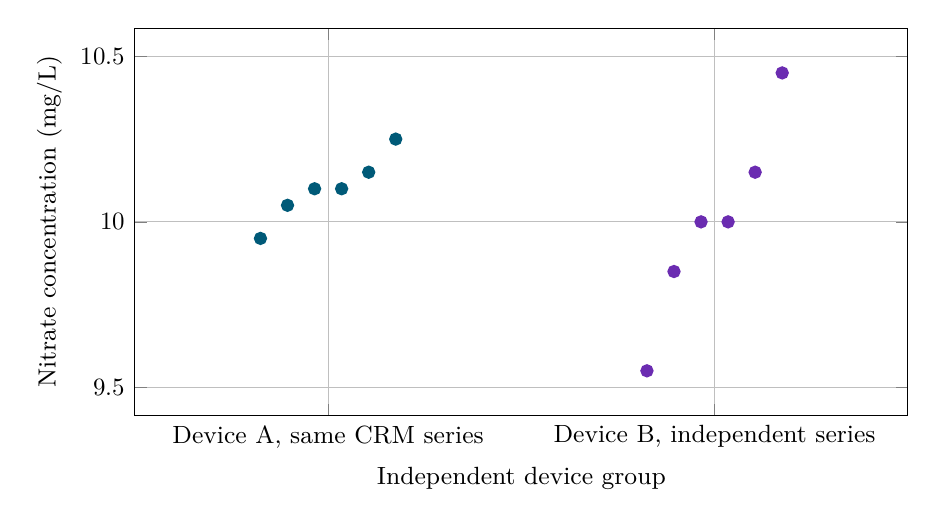
\begin{tikzpicture}
\begin{axis}[width=0.94\linewidth,
height=6.5cm,
scale only axis=false,
grid=major,
tick label style={font=\small},
label style={font=\small},
xlabel={Independent device group},
ylabel={Nitrate concentration (mg/L)},
legend style={font=\footnotesize,draw=none,at={(0.5,-0.28)},anchor=north,legend columns=1,text width=0.85\linewidth,align=left},
unbounded coords=jump,
scaled ticks=false,
ymin=9.415000000000001,
ymax=10.584999999999999,
xmin=0.5,
xmax=2.5,
xtick={1,2},
xticklabels={{Device A, same CRM series},{Device B, independent series}}]
\addplot[color=pcd1,thick,only marks,mark=*] coordinates {(0.825,9.95) (0.895,10.05) (0.965,10.1) (1.035,10.1) (1.105,10.15) (1.175,10.25)};
\addplot[color=pcd2,thick,only marks,mark=*] coordinates {(1.825,9.55) (1.895,9.85) (1.965,10) (2.035,10) (2.105,10.15) (2.175,10.45)};

\end{axis}
\end{tikzpicture}
\end{center}


\medskip

The numerator and denominator play different roles. Reversing their order reciprocates the ratio and exchanges the associated degrees of freedom. A pre-specified right-tail comparison therefore names the numerator group and the direction of the question before interpreting the observed variances.


When the true population variances are equal, they cancel in the normalized construction, leaving the corresponding sample-variance ratio as an F reference statistic. With unequal true variances, their true variance ratio scales the sample ratio. The displayed normalization makes this dependence explicit.


The normalized construction in \hyperref[material-069573de86e2978030e9cec76a253534ca1bd49fa6f892f3c4ee96c865021397]{Eq.~\ref*{material-069573de86e2978030e9cec76a253534ca1bd49fa6f892f3c4ee96c865021397}} leads to the concrete ordered ratio in \hyperref[material-e905ae6fc3128ed247268906a77342417dc4501089cc4016db512e589f2325d8]{Eq.~\ref*{material-e905ae6fc3128ed247268906a77342417dc4501089cc4016db512e589f2325d8}}. The relation in \hyperref[material-08a9ac12ea7fb14b07e9557de8a815133ecb6d81c265ba155e656d924fed69d4]{Eq.~\ref*{material-08a9ac12ea7fb14b07e9557de8a815133ecb6d81c265ba155e656d924fed69d4}} identifies the role of the true variance ratio, while \hyperref[material-d512e279368eaad47f7be8d444067461eb0aef51e8da53fc030a2f206e8ef865]{Fig.~\ref*{material-d512e279368eaad47f7be8d444067461eb0aef51e8da53fc030a2f206e8ef865}} shows repeated sample-variance ratios under equal true variances. Changing the sample sizes changes the two degrees-of-freedom parameters. Under the population and independence assumptions, the reference distribution describes variation in estimated spreads. Understanding this construction connects the F curve directly to the analytical comparison.


\par\medskip
\noindent\begin{minipage}{\linewidth}
\refstepcounter{equation}\label{material-069573de86e2978030e9cec76a253534ca1bd49fa6f892f3c4ee96c865021397}
\noindent\textbf{Eq.~\ref*{material-069573de86e2978030e9cec76a253534ca1bd49fa6f892f3c4ee96c865021397}.} An F variable constructed from two independent Normal-sample variance estimates.\par\nopagebreak
\begin{center}\begin{adjustbox}{max width=\linewidth}$\displaystyle F=\frac{S_B^2/\sigma_B^2}{S_A^2/\sigma_A^2}$\end{adjustbox}\end{center}

\par\noindent\textbf{Symbols}

\begin{itemize}\setlength{\itemsep}{1pt}\setlength{\parsep}{0pt}
\item \textbf{F}: Random normalized variance ratio (dimensionless).
\item \textbf{A, B}: Independent groups; B is the numerator and A the denominator.
\item \textbf{\(S_B^2, S_A^2\)}: Random sample variances about each group's estimated mean (\(\mathrm{(mg/L)^2}\)).
\item \textbf{\(σ_B^2, σ_A^2\)}: Corresponding fixed positive population variances (\(\mathrm{(mg/L)^2}\)).
\item \textbf{\ensuremath{{}^2}}: Square an SD to obtain variance.
\item \textbf{/}: Inner divisions normalize each sample variance; the outer fraction forms B/A.
\item \textbf{=}: Equality defining F.
\end{itemize}

Conditions: measurements are independent and identically Normal within each group, and the groups are independent. Group means may differ. Each variance uses divisor sample count minus one; six measurements per group give five degrees of freedom each. Equal true variances cancel, leaving the sample-variance ratio.

\end{minipage}\par
\medskip

\par\medskip
\noindent\begin{minipage}{\linewidth}
\refstepcounter{equation}\label{material-e905ae6fc3128ed247268906a77342417dc4501089cc4016db512e589f2325d8}
\noindent\textbf{Eq.~\ref*{material-e905ae6fc3128ed247268906a77342417dc4501089cc4016db512e589f2325d8}.} The observed ordered sample-variance ratio for the two measurement groups.\par\nopagebreak
\begin{center}\begin{adjustbox}{max width=\linewidth}$\displaystyle f=\frac{s_B^2}{s_A^2}=\frac{0.090}{0.010}=9$\end{adjustbox}\end{center}

\par\noindent\textbf{Symbols}

\begin{itemize}\setlength{\itemsep}{1pt}\setlength{\parsep}{0pt}
\item \textbf{f}: Observed sample-variance ratio (dimensionless).
\item \textbf{\(s_B^2\)}: Observed variance in group B, \(0.090\,\mathrm{(mg/L)^2}\).
\item \textbf{\(s_A^2\)}: Observed variance in group A, \(0.010\,\mathrm{(mg/L)^2}\).
\item \textbf{B, A}: Group subscripts specifying the prespecified numerator and denominator.
\item \textbf{\ensuremath{{}^2}, /, =}: Squaring an SD to obtain variance, division and equality.
\end{itemize}

Each group contains six independent results, with independent groups. Each variance uses that group's fitted mean and divisor five. Concentration units cancel in B/A; the group order is fixed before inspecting the data.

\end{minipage}\par
\medskip

\par\medskip
\noindent\begin{minipage}{\linewidth}
\refstepcounter{equation}\label{material-08a9ac12ea7fb14b07e9557de8a815133ecb6d81c265ba155e656d924fed69d4}
\noindent\textbf{Eq.~\ref*{material-08a9ac12ea7fb14b07e9557de8a815133ecb6d81c265ba155e656d924fed69d4}.} Normalization by the true variance ratio and the resulting ordered F reference.\par\nopagebreak
\begin{center}\begin{adjustbox}{max width=\linewidth}$\displaystyle Q_j=\frac{\nu_j S_j^2}{\sigma_j^2}\sim\chi^2_{\nu_j},\qquad F=\frac{Q_B/\nu_B}{Q_A/\nu_A}\sim F_{\nu_B,\nu_A}$\end{adjustbox}\end{center}

\par\noindent\textbf{Symbols}

\begin{itemize}\setlength{\itemsep}{1pt}\setlength{\parsep}{0pt}
\item \textbf{\(j\)}: Group index \(A\) or \(B\).
\item \textbf{\(ν_j\)}: Group \(j\)'s sample count minus one, giving its degrees of freedom.
\item \textbf{\(S_j^2\)}: Random sample variance about group \(j\)'s fitted mean (\(\mathrm{(mg/L)^2}\)).
\item \textbf{\(σ_j^2\)}: Positive true variance of group \(j\) (\(\mathrm{(mg/L)^2}\)).
\item \textbf{\(Q_j\)}: Scaled sample variance, \(\frac{ν_j S_j^2}{σ_j^2}\) (dimensionless).
\item \textbf{\(F\)}: Resulting dimensionless random ratio; also the name of its reference distribution.
\item \textbf{\(()^2, /, =, ∼\)}: Variance from squaring an SD; division; equality; follows the named distribution.
\item \textbf{Comma}: Orders distribution parameters: numerator B degrees of freedom, then denominator A.
\end{itemize}

The Normal samples and groups are independent, making \(Q_A\) and \(Q_B\) independent chi-square variables. Both degrees of freedom are five here. Equal true variances cancel; otherwise normalize the sample-variance ratio by the true \(B/A\) variance ratio.

\end{minipage}\par
\medskip

\par\medskip
\Needspace{10cm}
\refstepcounter{figure}\label{material-d512e279368eaad47f7be8d444067461eb0aef51e8da53fc030a2f206e8ef865}
\noindent\textbf{Fig.~\ref*{material-d512e279368eaad47f7be8d444067461eb0aef51e8da53fc030a2f206e8ef865}.} The histogram contains variance ratios B/A from 1,000 independent Normal sample pairs, with six measurements per group and equal true variances. The overlaid F density uses five numerator and five denominator degrees of freedom.\par\nopagebreak
\begin{center}
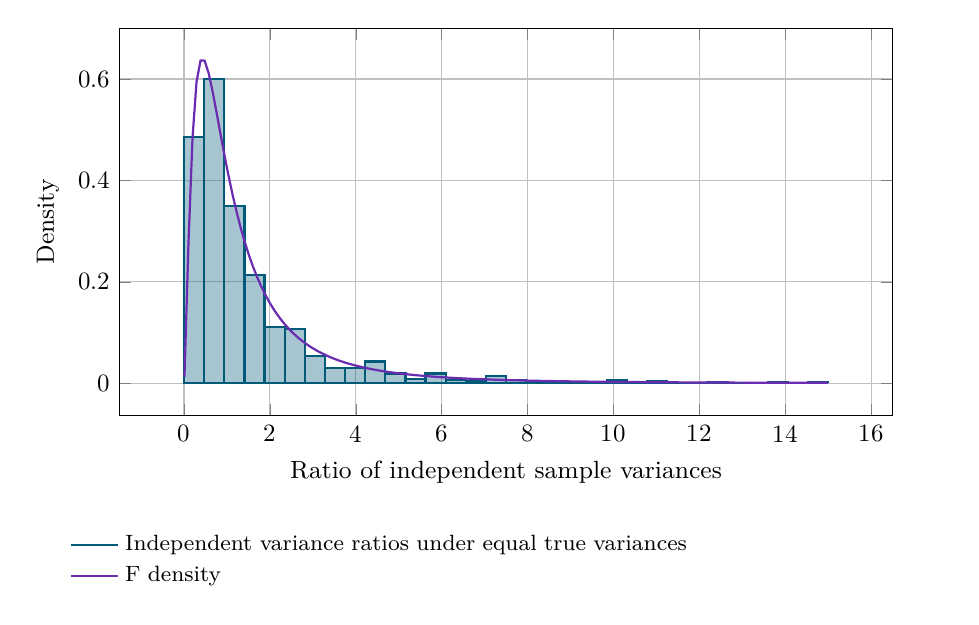
\begin{tikzpicture}
\begin{axis}[width=0.94\linewidth,
height=6.5cm,
scale only axis=false,
grid=major,
tick label style={font=\small},
label style={font=\small},
xlabel={Ratio of independent sample variances},
ylabel={Density},
legend style={font=\footnotesize,draw=none,at={(0.5,-0.28)},anchor=north,legend columns=1,text width=0.85\linewidth,align=left},
unbounded coords=jump,
scaled ticks=false]
\addplot[color=pcd1,thick,fill=pcd1,fill opacity=0.35,mark=none] coordinates {(0,0) (0,0.4864) (0.46875,0.4864) (0.46875,0)} \closedcycle;
\addplot[color=pcd1,thick,fill=pcd1,fill opacity=0.35,forget plot,mark=none] coordinates {(0.46875,0) (0.46875,0.5994666666666667) (0.9375,0.5994666666666667) (0.9375,0)} \closedcycle;
\addplot[color=pcd1,thick,fill=pcd1,fill opacity=0.35,forget plot,mark=none] coordinates {(0.9375,0) (0.9375,0.34986666666666666) (1.40625,0.34986666666666666) (1.40625,0)} \closedcycle;
\addplot[color=pcd1,thick,fill=pcd1,fill opacity=0.35,forget plot,mark=none] coordinates {(1.40625,0) (1.40625,0.21333333333333335) (1.875,0.21333333333333335) (1.875,0)} \closedcycle;
\addplot[color=pcd1,thick,fill=pcd1,fill opacity=0.35,forget plot,mark=none] coordinates {(1.875,0) (1.875,0.11093333333333333) (2.34375,0.11093333333333333) (2.34375,0)} \closedcycle;
\addplot[color=pcd1,thick,fill=pcd1,fill opacity=0.35,forget plot,mark=none] coordinates {(2.34375,0) (2.34375,0.10666666666666667) (2.8125,0.10666666666666667) (2.8125,0)} \closedcycle;
\addplot[color=pcd1,thick,fill=pcd1,fill opacity=0.35,forget plot,mark=none] coordinates {(2.8125,0) (2.8125,0.05333333333333334) (3.28125,0.05333333333333334) (3.28125,0)} \closedcycle;
\addplot[color=pcd1,thick,fill=pcd1,fill opacity=0.35,forget plot,mark=none] coordinates {(3.28125,0) (3.28125,0.029866666666666666) (3.75,0.029866666666666666) (3.75,0)} \closedcycle;
\addplot[color=pcd1,thick,fill=pcd1,fill opacity=0.35,forget plot,mark=none] coordinates {(3.75,0) (3.75,0.029866666666666666) (4.21875,0.029866666666666666) (4.21875,0)} \closedcycle;
\addplot[color=pcd1,thick,fill=pcd1,fill opacity=0.35,forget plot,mark=none] coordinates {(4.21875,0) (4.21875,0.042666666666666665) (4.6875,0.042666666666666665) (4.6875,0)} \closedcycle;
\addplot[color=pcd1,thick,fill=pcd1,fill opacity=0.35,forget plot,mark=none] coordinates {(4.6875,0) (4.6875,0.0192) (5.15625,0.0192) (5.15625,0)} \closedcycle;
\addplot[color=pcd1,thick,fill=pcd1,fill opacity=0.35,forget plot,mark=none] coordinates {(5.15625,0) (5.15625,0.008533333333333334) (5.625,0.008533333333333334) (5.625,0)} \closedcycle;
\addplot[color=pcd1,thick,fill=pcd1,fill opacity=0.35,forget plot,mark=none] coordinates {(5.625,0) (5.625,0.0192) (6.09375,0.0192) (6.09375,0)} \closedcycle;
\addplot[color=pcd1,thick,fill=pcd1,fill opacity=0.35,forget plot,mark=none] coordinates {(6.09375,0) (6.09375,0.0064) (6.5625,0.0064) (6.5625,0)} \closedcycle;
\addplot[color=pcd1,thick,fill=pcd1,fill opacity=0.35,forget plot,mark=none] coordinates {(6.5625,0) (6.5625,0.004266666666666667) (7.03125,0.004266666666666667) (7.03125,0)} \closedcycle;
\addplot[color=pcd1,thick,fill=pcd1,fill opacity=0.35,forget plot,mark=none] coordinates {(7.03125,0) (7.03125,0.014933333333333333) (7.5,0.014933333333333333) (7.5,0)} \closedcycle;
\addplot[color=pcd1,thick,fill=pcd1,fill opacity=0.35,forget plot,mark=none] coordinates {(7.5,0) (7.5,0.0064) (7.96875,0.0064) (7.96875,0)} \closedcycle;
\addplot[color=pcd1,thick,fill=pcd1,fill opacity=0.35,forget plot,mark=none] coordinates {(7.96875,0) (7.96875,0.004266666666666667) (8.4375,0.004266666666666667) (8.4375,0)} \closedcycle;
\addplot[color=pcd1,thick,fill=pcd1,fill opacity=0.35,forget plot,mark=none] coordinates {(8.4375,0) (8.4375,0) (8.90625,0) (8.90625,0)} \closedcycle;
\addplot[color=pcd1,thick,fill=pcd1,fill opacity=0.35,forget plot,mark=none] coordinates {(8.90625,0) (8.90625,0.0021333333333333334) (9.375,0.0021333333333333334) (9.375,0)} \closedcycle;
\addplot[color=pcd1,thick,fill=pcd1,fill opacity=0.35,forget plot,mark=none] coordinates {(9.375,0) (9.375,0) (9.84375,0) (9.84375,0)} \closedcycle;
\addplot[color=pcd1,thick,fill=pcd1,fill opacity=0.35,forget plot,mark=none] coordinates {(9.84375,0) (9.84375,0.0064) (10.3125,0.0064) (10.3125,0)} \closedcycle;
\addplot[color=pcd1,thick,fill=pcd1,fill opacity=0.35,forget plot,mark=none] coordinates {(10.3125,0) (10.3125,0.0021333333333333334) (10.78125,0.0021333333333333334) (10.78125,0)} \closedcycle;
\addplot[color=pcd1,thick,fill=pcd1,fill opacity=0.35,forget plot,mark=none] coordinates {(10.78125,0) (10.78125,0.004266666666666667) (11.25,0.004266666666666667) (11.25,0)} \closedcycle;
\addplot[color=pcd1,thick,fill=pcd1,fill opacity=0.35,forget plot,mark=none] coordinates {(11.25,0) (11.25,0) (11.71875,0) (11.71875,0)} \closedcycle;
\addplot[color=pcd1,thick,fill=pcd1,fill opacity=0.35,forget plot,mark=none] coordinates {(11.71875,0) (11.71875,0) (12.1875,0) (12.1875,0)} \closedcycle;
\addplot[color=pcd1,thick,fill=pcd1,fill opacity=0.35,forget plot,mark=none] coordinates {(12.1875,0) (12.1875,0.0021333333333333334) (12.65625,0.0021333333333333334) (12.65625,0)} \closedcycle;
\addplot[color=pcd1,thick,fill=pcd1,fill opacity=0.35,forget plot,mark=none] coordinates {(12.65625,0) (12.65625,0) (13.125,0) (13.125,0)} \closedcycle;
\addplot[color=pcd1,thick,fill=pcd1,fill opacity=0.35,forget plot,mark=none] coordinates {(13.125,0) (13.125,0) (13.59375,0) (13.59375,0)} \closedcycle;
\addplot[color=pcd1,thick,fill=pcd1,fill opacity=0.35,forget plot,mark=none] coordinates {(13.59375,0) (13.59375,0.0021333333333333334) (14.0625,0.0021333333333333334) (14.0625,0)} \closedcycle;
\addplot[color=pcd1,thick,fill=pcd1,fill opacity=0.35,forget plot,mark=none] coordinates {(14.0625,0) (14.0625,0) (14.53125,0) (14.53125,0)} \closedcycle;
\addplot[color=pcd1,thick,fill=pcd1,fill opacity=0.35,forget plot,mark=none] coordinates {(14.53125,0) (14.53125,0.0021333333333333334) (15,0.0021333333333333334) (15,0)} \closedcycle;
\addlegendentry{Independent variance ratios under equal true variances}
\addplot[color=pcd2,thick,mark=none] coordinates {(0.01,0.012922066548475093) (0.1036875,0.27688397922444) (0.19737500000000002,0.4838671352914428) (0.2910625,0.5945411116983244) (0.38475000000000004,0.6365754942275629) (0.4784375,0.6362998372558862) (0.572125,0.611983708124159) (0.6658125,0.5752229110153441) (0.7595000000000001,0.5330698914894374) (0.8531875,0.4896759306648766) (0.946875,0.44739123951648396) (1.0405625,0.40746620273077416) (1.13425,0.3704892180324667) (1.2279375000000001,0.33665744151322763) (1.321625,0.3059432327529256) (1.4153125,0.2781958908639561) (1.5090000000000001,0.2532033196943902) (1.6026875,0.23072889457826512) (1.696375,0.21053299966694708) (1.7900625000000001,0.19238511809670067) (1.88375,0.17607013716819797) (1.9774375000000002,0.16139115199273327) (2.071125,0.14817019145105043) (2.1648124999999996,0.13624775231592448) (2.2584999999999997,0.12548168963459141) (2.3521875,0.11574579901563094) (2.445875,0.10692829279648937) (2.5395624999999997,0.09893028813523427) (2.63325,0.09166437263316546) (2.7269374999999996,0.08505328063923849) (2.8206249999999997,0.07902869361026546) (2.9143125,0.07353016615333959) (3.008,0.06850417269050726) (3.1016874999999997,0.06390326616225009) (3.195375,0.05968533861194637) (3.2890624999999996,0.05581297309342989) (3.3827499999999997,0.05225287662573466) (3.4764375,0.04897538457276251) (3.570125,0.045954027657735444) (3.6638124999999997,0.04316515371504899) (3.7575,0.04058759716585776) (3.8511875,0.03820239003939153) (3.944875,0.0359925091298528) (4.0385625,0.033942654570865975) (4.13225,0.03203905572508104) (4.2259375,0.030269300828963144) (4.319624999999999,0.0286221873075035) (4.4133125,0.027087590086977763) (4.507,0.02565634559260966) (4.600687499999999,0.024320149428515424) (4.694375,0.02307146600563905) (4.7880625,0.0219034486150042) (4.88175,0.02080986864341696) (4.9754375,0.019785052801074503) (5.069125,0.01882382737916277) (5.1628125,0.017921468683752977) (5.2565,0.017073658902994407) (5.3501875000000005,0.016276446760201208) (5.443874999999999,0.015526212388076574) (5.5375625,0.014819635930813303) (5.63125,0.014153669442733191) (5.724937499999999,0.013525511705803605) (5.818625,0.012932585634954565) (5.9123125,0.012372517980592773) (6.006,0.011843121072911938) (6.0996875,0.011342376383256317) (6.193375,0.010868419704522334) (6.2870625,0.010419527775915918) (6.38075,0.009994106197775549) (6.4744375,0.009590678500014004) (6.568124999999999,0.009207876243366685) (6.6618125,0.008844430046347117) (6.7555,0.008499161442853394) (6.849187499999999,0.008170975485960677) (6.942875,0.007858854022756693) (7.0365625,0.007561849573294898) (7.13025,0.007279079753991121) (7.2239375,0.007009722192195472) (7.317625,0.006753009884337775) (7.4113125,0.00650822695506158) (7.505,0.006274704779210025) (7.5986875000000005,0.006051818432473717) (7.692375,0.005838983440017891) (7.7860625,0.0056356527955254265) (7.8797500000000005,0.005441314225869026) (7.9734375,0.005255487679101447) (8.067125,0.005077723015661259) (8.1608125,0.004907597884663663) (8.2545,0.004744715768910403) (8.3481875,0.004588704183829812) (8.441875,0.004439213016973205) (8.5355625,0.004295912995960556) (8.629249999999999,0.004158494273907149) (8.722937499999999,0.004026665122384526) (8.816625,0.0039001507228887547) (8.9103125,0.003778692048616362) (9.004,0.0036620448290933766) (9.0976875,0.0035499785908752975) (9.191374999999999,0.003442275768142279) (9.2850625,0.003338730877561212) (9.37875,0.0032391497522822827) (9.4724375,0.0031433488303847894) (9.566125,0.003051154493493565) (9.6598125,0.0029624024516541458) (9.7535,0.002876937170888869) (9.8471875,0.0027946113401584737) (9.940875,0.0027152853747285524) (10.0345625,0.0026388269531904545) (10.12825,0.0025651105856132257) (10.221937500000001,0.0024940172105103907) (10.315625,0.0024254338184937865) (10.4093125,0.002359253100658791) (10.503,0.0022953731199018583) (10.5966875,0.0022336970035148726) (10.690375000000001,0.0021741326555312916) (10.784062500000001,0.002116592487419031) (10.877749999999999,0.0020609931658242212) (10.971437499999999,0.002007255376170416) (11.065125,0.001955303601009392) (11.1588125,0.0019050659121041058) (11.2525,0.0018564737753012023) (11.3461875,0.0018094618673217032) (11.439874999999999,0.0017639679036632835) (11.5335625,0.0017199324768674342) (11.62725,0.0016772989044598744) (11.7209375,0.0016360130859229246) (11.814625,0.001596023368105459) (11.9083125,0.0015572804185185803) (12.002,0.0015197371060050335) (12.0956875,0.0014833483883065735) (12.189375,0.0014480712060872844) (12.2830625,0.0014138643830018678) (12.37675,0.0013806885314265628) (12.470437500000001,0.001348505963496957) (12.564125,0.0013172806071213826) (12.6578125,0.0012869779266612494) (12.7515,0.001257564847990768) (12.8451875,0.0012290096876679001) (12.938875,0.0012012820859662735) (13.032562500000001,0.0011743529435347235) (13.126249999999999,0.0011481943614663778) (13.2199375,0.0011227795845737438) (13.313625,0.0010980829476794896) (13.407312500000002,0.0010740798247450534) (13.501,0.0010507465806706988) (13.594687500000001,0.001028060525611364) (13.688374999999999,0.0010059998716625731) (13.7820625,0.000984543691779975) (13.87575,0.0009636718808046623) (13.969437500000002,0.000943365118474495) (14.063125,0.0009236048343090588) (14.156812500000001,0.0009043731742629801) (14.2505,0.0008856529690486726) (14.344187500000002,0.0008674277040358003) (14.437875,0.0008496814906403086) (14.531562499999998,0.0008323990391211594) (14.62525,0.0008155656327079499) (14.7189375,0.0007991671029870211) (14.812625,0.0007831898064781847) (14.906312499999999,0.00076762060233804) (15,0.0007524468311297561)};
\addlegendentry{F density}

\end{axis}
\end{tikzpicture}
\end{center}

% Full-precision experiment details: {"blockId":"ex:rv-f-v--block","parameters":[{"key":"nA","label":"Hypothetical measurements in A","value":6},{"key":"nB","label":"Hypothetical measurements in B","value":6},{"key":"sigma","label":"True method SD (mg/L), assumed","value":0.1},{"key":"M","label":"Simulated complete series","value":1000},{"key":"seed","label":"Replay seed (Park-Miller)","value":20261102},{"key":"reverse","label":"Ratio direction: 0 B/A, 1 A/B","value":0},{"key":"view","label":"Distribution construction and ordered degrees of freedom","value":3}],"readouts":[{"label":"Numerator df","value":5},{"label":"Denominator df","value":5},{"label":"Simulated complete pairs","value":1000}],"note":"Independent Normal samples with equal true variances produce this sample-variance ratio. More generally, divide each variance by its own true variance before forming the ratio. The population means may differ. Reversing the ratio swaps numerator and denominator degrees of freedom. The positive support extends to infinity; the drawing shows a finite window.","markers":[[]]}

\medskip

\clearpage
\section{Connecting distribution families through their constructions}
The five families can now be connected through the operations that generate their random quantities. Additive contributions motivate a Normal approximation under suitable conditions; multiplicative positive factors motivate a Normal log ratio and hence a lognormal concentration. Squared independent standard-Normal components yield chi-square quantities. Standardizing a Normal sample mean by an estimated standard error yields t, while ratios of independent normalized variance estimates yield F.


These constructions connect the model assumptions with the quantity being studied. A Normal model for individual results and a chi-square model for their scaled sample variance describe different aspects of the same repeated experiment. The t reference describes the standardized sample mean when its standard error is estimated.


The compact formula collection keeps these relationships together with their complete symbol definitions. The additive construction in \hyperref[material-05c01eaec154fbc338a6201e6d9f7cd0a102f80069edbf86f837df275027c6e8]{Eq.~\ref*{material-05c01eaec154fbc338a6201e6d9f7cd0a102f80069edbf86f837df275027c6e8}} and multiplicative construction in \hyperref[material-b2e4e5f1274b53286172c117d5653f1c07de7f18cbb621f6513b852f7dd1421d]{Eq.~\ref*{material-b2e4e5f1274b53286172c117d5653f1c07de7f18cbb621f6513b852f7dd1421d}} describe individual results. The scaled variance in \hyperref[material-e7b6a30cd73c439e84ba5ae89f306ba199f7b753521cdf3ebe6e3fc08233d388]{Eq.~\ref*{material-e7b6a30cd73c439e84ba5ae89f306ba199f7b753521cdf3ebe6e3fc08233d388}}, studentized mean in \hyperref[material-becb108ac77c9ad56c4b8c28113dbde3cf647df7ecee3b2690d7d606834bbad2]{Eq.~\ref*{material-becb108ac77c9ad56c4b8c28113dbde3cf647df7ecee3b2690d7d606834bbad2}} and normalized variance ratio in \hyperref[material-9887499761e2748bbe479a2a69352646568e3dc59eaf1222507d6ced265c625f]{Eq.~\ref*{material-9887499761e2748bbe479a2a69352646568e3dc59eaf1222507d6ced265c625f}} describe statistics of complete samples. To choose a reference, first identify what is random and what has been estimated, then establish the assumptions that justify the construction. This leads to the final task: checking how closely observed data agree with a proposed model.


\par\medskip
\noindent\begin{minipage}{\linewidth}
\refstepcounter{equation}\label{material-05c01eaec154fbc338a6201e6d9f7cd0a102f80069edbf86f837df275027c6e8}
\noindent\textbf{Eq.~\ref*{material-05c01eaec154fbc338a6201e6d9f7cd0a102f80069edbf86f837df275027c6e8}.} Additive contributions and the Normal approximation under central-limit conditions.\par\nopagebreak
\begin{center}\begin{adjustbox}{max width=\linewidth}$\displaystyle Y=X_1+X_2+X_3+\cdots$\end{adjustbox}\end{center}

\par\noindent\textbf{Symbols}

\begin{itemize}\setlength{\itemsep}{1pt}\setlength{\parsep}{0pt}
\item \textbf{Y}: Random total concentration contribution (mg/L).
\item \textbf{X\ensuremath{{}_1}, X\ensuremath{{}_2}, X\ensuremath{{}_3}}: Random additive contributions, such as injection, flow and detector effects (mg/L).
\item \textbf{1, 2, 3}: Subscripts identifying the contributions.
\item \textbf{+}: Addition.
\item \textbf{\ensuremath{\ldots}, =}: Continuation of the finite sum; equality defining Y.
\end{itemize}

Independent Normal contributions give an exact Normal sum. A central-limit approximation requires suitable conditions, including finite variances and control of the individual contributions relative to the total variation.

\end{minipage}\par
\medskip

\par\medskip
\noindent\begin{minipage}{\linewidth}
\refstepcounter{equation}\label{material-b2e4e5f1274b53286172c117d5653f1c07de7f18cbb621f6513b852f7dd1421d}
\noindent\textbf{Eq.~\ref*{material-b2e4e5f1274b53286172c117d5653f1c07de7f18cbb621f6513b852f7dd1421d}.} Multiplicative positive factors represented by a Normal log ratio.\par\nopagebreak
\begin{center}\begin{adjustbox}{max width=\linewidth}$\displaystyle Y=X_1\cdot X_2\cdot X_3\cdots$\end{adjustbox}\end{center}

\par\noindent\textbf{Symbols}

\begin{itemize}\setlength{\itemsep}{1pt}\setlength{\parsep}{0pt}
\item \textbf{Y}: Positive random total relative factor (dimensionless).
\item \textbf{X\ensuremath{{}_1}, X\ensuremath{{}_2}, X\ensuremath{{}_3}}: Positive random relative factors (dimensionless); subscripts identify the factors.
\item \textbf{\ensuremath{\cdot}}: Multiplication of factors.
\item \textbf{\ensuremath{\ldots}, =}: Continuation of the finite product; equality defining Y.
\end{itemize}

Condition: the sum of natural-log factors is Normal; independent Normal log factors suffice. Multiplying Y by a fixed reference concentration restores concentration units.

\end{minipage}\par
\medskip

\par\medskip
\noindent\begin{minipage}{\linewidth}
\refstepcounter{equation}\label{material-e7b6a30cd73c439e84ba5ae89f306ba199f7b753521cdf3ebe6e3fc08233d388}
\noindent\textbf{Eq.~\ref*{material-e7b6a30cd73c439e84ba5ae89f306ba199f7b753521cdf3ebe6e3fc08233d388}.} The scaled Normal-sample variance and its chi-square reference.\par\nopagebreak
\begin{center}\begin{adjustbox}{max width=\linewidth}$\displaystyle \begin{gathered}Q=Z_1^2+\cdots+Z_\nu^2\\Q=\frac{(n-1)S^2}{\sigma^2}\end{gathered}$\end{adjustbox}\end{center}

\par\noindent\textbf{Symbols}

\begin{itemize}\setlength{\itemsep}{1pt}\setlength{\parsep}{0pt}
\item \textbf{Q}: Chi-square random variable (dimensionless).
\item \textbf{Z\ensuremath{{}_i}}: Independent standard-normal component i, with mean zero and variance one.
\item \textbf{\(ν\)}: Positive integer number of degrees of freedom; the last component is \(Z_ν\).
\item \textbf{n}: Number of independent, identically distributed Normal measurements, at least two.
\item \textbf{S\ensuremath{{}^2}}: Sample variance about the estimated mean, using divisor n \ensuremath{-} 1 ((mg/L)\ensuremath{{}^2}).
\item \textbf{\ensuremath{\sigma}\ensuremath{{}^2}}: Positive true population variance ((mg/L)\ensuremath{{}^2}).
\item \textbf{\ensuremath{{}^2}, +, \ensuremath{\ldots}}: Squaring, addition and continuation through all \ensuremath{\nu} components.
\item \textbf{\ensuremath{-}, /, =}: Subtraction, division and equality; adjacent factors multiply.
\end{itemize}

For sample variance, \ensuremath{\nu} = n \ensuremath{-} 1. Scaling cancels concentration units. Independent Z components correspond to orthonormal residual coordinates; the raw centred residuals share the fitted mean.

\end{minipage}\par
\medskip

\par\medskip
\noindent\begin{minipage}{\linewidth}
\refstepcounter{equation}\label{material-becb108ac77c9ad56c4b8c28113dbde3cf647df7ecee3b2690d7d606834bbad2}
\noindent\textbf{Eq.~\ref*{material-becb108ac77c9ad56c4b8c28113dbde3cf647df7ecee3b2690d7d606834bbad2}.} A sample mean standardized with its estimated standard error and the Student t reference.\par\nopagebreak
\begin{center}\begin{adjustbox}{max width=\linewidth}$\displaystyle T=\frac{\bar X-\mu}{S/\sqrt n}$\end{adjustbox}\end{center}

\par\noindent\textbf{Symbols}

\begin{itemize}\setlength{\itemsep}{1pt}\setlength{\parsep}{0pt}
\item \textbf{T}: Random Student variable (dimensionless).
\item \textbf{\ensuremath{\bar{X}}}: Random sample mean (mg/L); the bar denotes averaging.
\item \textbf{\ensuremath{\mu}}: Fixed true population mean (mg/L).
\item \textbf{S}: Positive sample SD from the same measurements (mg/L).
\item \textbf{n}: Sample count, at least two.
\item \textbf{S / \ensuremath{\sqrt{\vphantom{x}}}n}: Estimated standard error of the mean (mg/L); the square root is positive.
\item \textbf{\ensuremath{-}, /, =}: Centre the mean, divide its departure by the standard error, and define T.
\end{itemize}

Condition: independent, identically distributed Normal measurements. Sample variance uses divisor n \ensuremath{-} 1, giving n \ensuremath{-} 1 Student degrees of freedom.

\end{minipage}\par
\medskip

\par\medskip
\noindent\begin{minipage}{\linewidth}
\refstepcounter{equation}\label{material-9887499761e2748bbe479a2a69352646568e3dc59eaf1222507d6ced265c625f}
\noindent\textbf{Eq.~\ref*{material-9887499761e2748bbe479a2a69352646568e3dc59eaf1222507d6ced265c625f}.} Independent variance estimates normalized to form an F variable.\par\nopagebreak
\begin{center}\begin{adjustbox}{max width=\linewidth}$\displaystyle F=\frac{S_B^2/\sigma_B^2}{S_A^2/\sigma_A^2}$\end{adjustbox}\end{center}

\par\noindent\textbf{Symbols}

\begin{itemize}\setlength{\itemsep}{1pt}\setlength{\parsep}{0pt}
\item \textbf{F}: Random normalized variance ratio (dimensionless).
\item \textbf{\(S_B^2, S_A^2\)}: Random sample variances in groups B and A (\(\mathrm{(mg/L)^2}\)).
\item \textbf{\(σ_B^2, σ_A^2\)}: Corresponding positive true population variances (\(\mathrm{(mg/L)^2}\)).
\item \textbf{A, B}: Independent groups; B supplies the numerator and A the denominator.
\item \textbf{\ensuremath{{}^2}}: Squaring an SD to obtain variance.
\item \textbf{/, =}: Inner fractions normalize each variance; the outer fraction forms the ratio; equality defines F.
\end{itemize}

Within each group, measurements are independent and identically Normal; group means may differ. Each sample variance uses its fitted mean and divisor sample count minus one. Ordered degrees of freedom are B count minus one, then A count minus one. Equal true variances cancel.

\end{minipage}\par
\medskip

\clearpage
\section{Assessing agreement between observations and a model}
Model assessment compares observed results with the patterns predicted by a proposed distribution. Quantile-quantile plots compare the ordered observations with theoretical quantiles. The resulting pattern helps identify agreement and departures in location, spread or shape, interpreted in the context of sample size and measurement conditions.


The two constructed five-result examples use the same Normal model fixed in advance. Their Q-Q comparison is shown in \hyperref[material-13e6591841bad6c1a38b5b47a1bc0660efd16c36fa3af95383c4006596596906]{Fig.~\ref*{material-13e6591841bad6c1a38b5b47a1bc0660efd16c36fa3af95383c4006596596906}}. The graphical comparisons and the following Kolmogorov-Smirnov calculation therefore address one consistent reference. The KS distance is the largest vertical difference between the empirical and theoretical CDFs, evaluated on both sides of every empirical jump; \hyperref[material-48b55b17bda94fcebe7c242ce86272123f5778a9bc94361ad75260966f8d1d46]{Fig.~\ref*{material-48b55b17bda94fcebe7c242ce86272123f5778a9bc94361ad75260966f8d1d46}} shows where those distances occur.


\par\medskip
\Needspace{10cm}
\refstepcounter{figure}\label{material-13e6591841bad6c1a38b5b47a1bc0660efd16c36fa3af95383c4006596596906}
\noindent\textbf{Fig.~\ref*{material-13e6591841bad6c1a38b5b47a1bc0660efd16c36fa3af95383c4006596596906}.} Both Q-Q panels use the Normal model with expectation 10 mg/L and SD 0.50 mg/L fixed before observing either five-result sample. Sample A lies close to the identity line; sample B bends toward its extreme upper observation.\par\nopagebreak
\begin{center}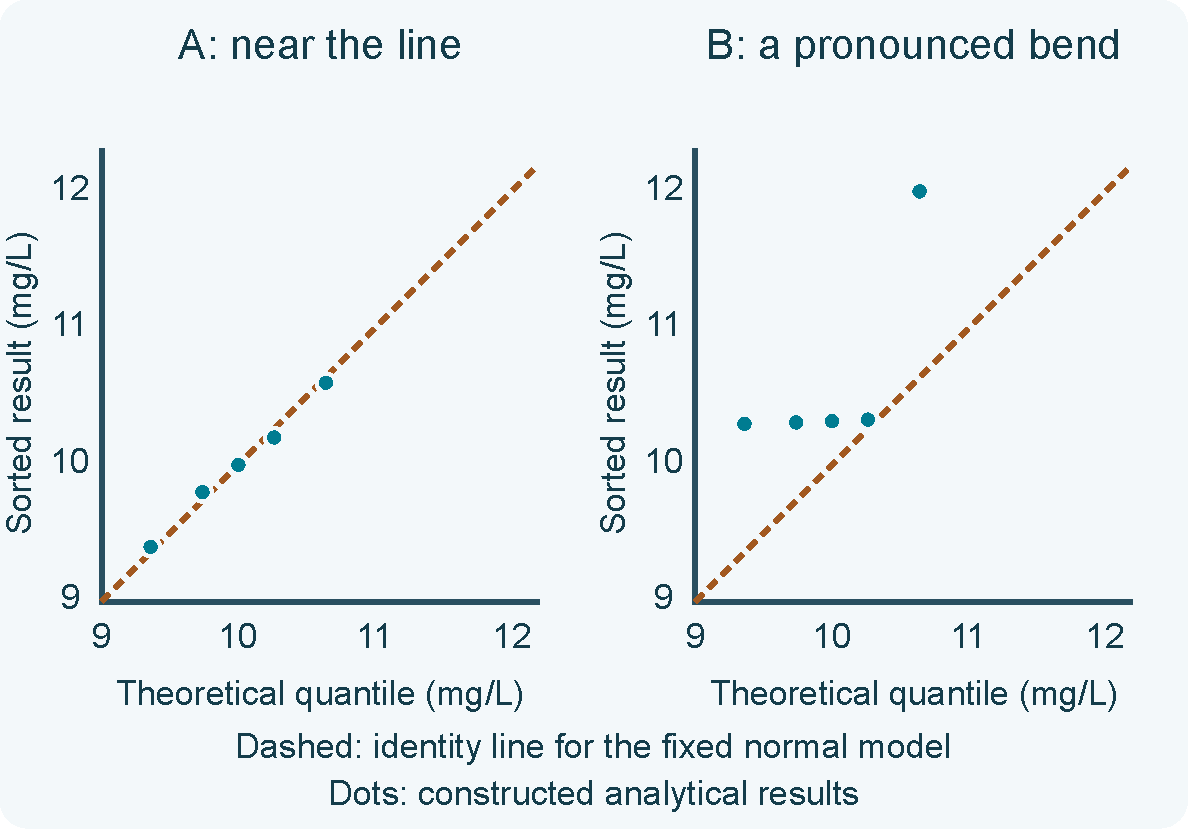
\includegraphics[width=\linewidth,height=.62\textheight,keepaspectratio]{asset-03662e534b4fea74e6a31b9eaa5d7a6c5ff7ac1afc5f54be6b6875804641f360.pdf}\end{center}

\medskip

\par\medskip
\Needspace{10cm}
\refstepcounter{figure}\label{material-48b55b17bda94fcebe7c242ce86272123f5778a9bc94361ad75260966f8d1d46}
\noindent\textbf{Fig.~\ref*{material-48b55b17bda94fcebe7c242ce86272123f5778a9bc94361ad75260966f8d1d46}.} The ECDFs and fixed Normal CDF (expectation 10 mg/L, SD 0.50 mg/L) use common concentration axes. Vertical gaps include both sides of each empirical jump; maximum distances are 0.144578 for A and 0.725747 for B.\par\nopagebreak
\begin{center}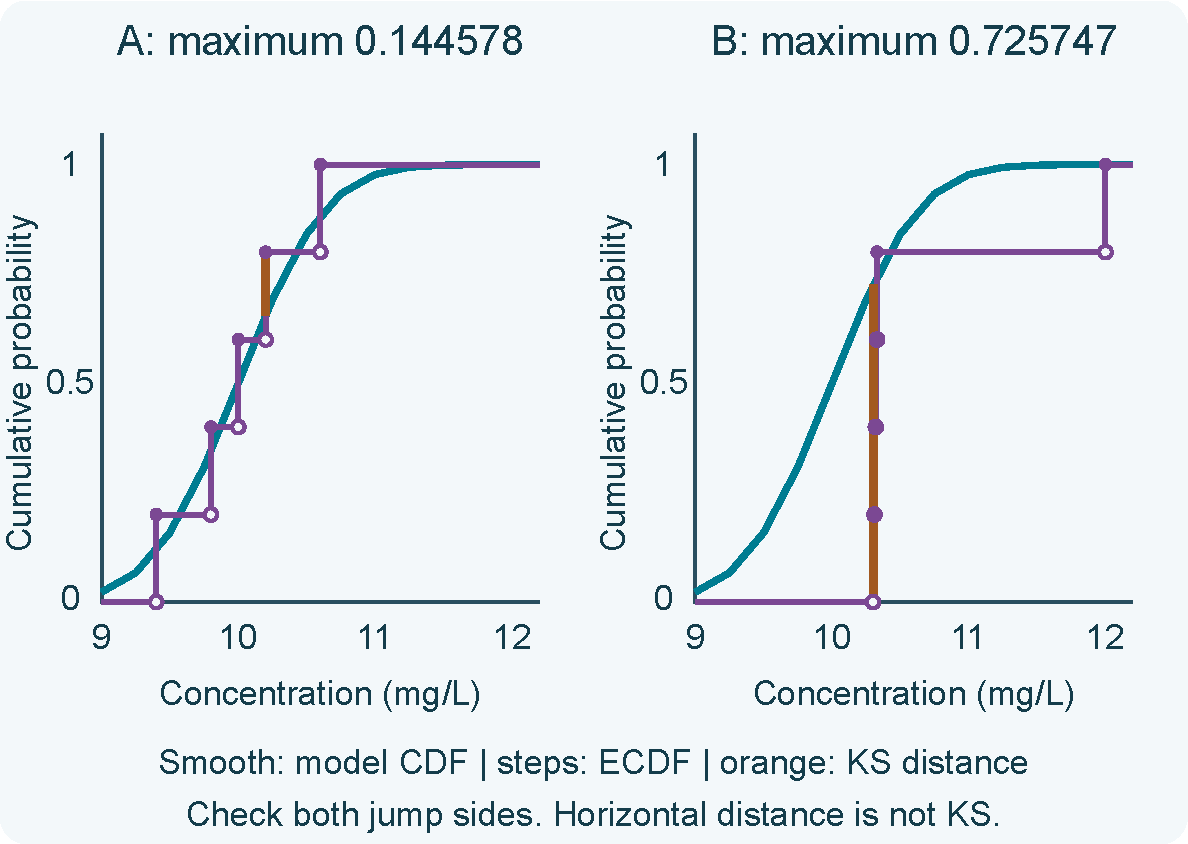
\includegraphics[width=\linewidth,height=.62\textheight,keepaspectratio]{asset-72c37de8a8c3e32d99300889433d08020df32131f2a639211c798d877d599152.pdf}\end{center}

\medskip

For a continuous null model fixed before observing the data, the exact five-observation two-sided cutoff at the stated significance level is about 0.563275. The first example falls below this cutoff and the deliberately skewed second example exceeds it. Estimating location or spread from the observations requires a calibration suited to that fitted-model setup, such as an applicable Lilliefors procedure or a correctly refitted bootstrap.


Pearson's goodness-of-fit calculation takes a grouped view. Expected bin counts come from model probabilities at the actual bin boundaries, including the specified tails. Observed and expected particle counts are compared directly in \hyperref[material-207fd4ff17aafed853b6da7de4012d0da7af8f4e9f31054e5b3588783fae814a]{Fig.~\ref*{material-207fd4ff17aafed853b6da7de4012d0da7af8f4e9f31054e5b3588783fae814a}}. Each bin contributes a squared observed-minus-expected difference divided by its expected count. Their sum is the test statistic, and the contribution plot shows how each group contributes to the overall discrepancy.


\par\medskip
\Needspace{10cm}
\refstepcounter{figure}\label{material-207fd4ff17aafed853b6da7de4012d0da7af8f4e9f31054e5b3588783fae814a}
\noindent\textbf{Fig.~\ref*{material-207fd4ff17aafed853b6da7de4012d0da7af8f4e9f31054e5b3588783fae814a}.} Observed counts for 100 particles in five fixed diameter categories are compared with expected counts 10, 20, 40, 20 and 10. The highlighted reference points show the fixed expectations.\par\nopagebreak
\begin{center}
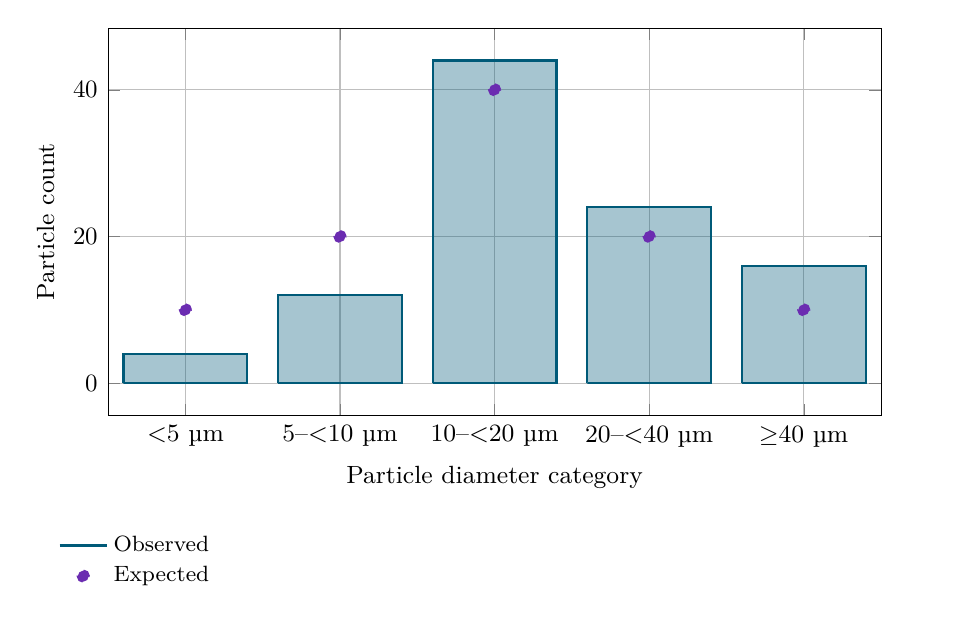
\begin{tikzpicture}
\begin{axis}[width=0.94\linewidth,
height=6.5cm,
scale only axis=false,
grid=major,
tick label style={font=\small},
label style={font=\small},
xlabel={Particle diameter category},
ylabel={Particle count},
legend style={font=\footnotesize,draw=none,at={(0.5,-0.28)},anchor=north,legend columns=1,text width=0.85\linewidth,align=left},
unbounded coords=jump,
scaled ticks=false,
xmin=0.5,
xmax=5.5,
xtick={1,2,3,4,5},
xticklabels={{<5 µm},{5–<10 µm},{10–<20 µm},{20–<40 µm},{\ensuremath{\ge}40 µm}}]
\addplot[color=pcd1,thick,fill=pcd1,fill opacity=0.35,mark=none] coordinates {(0.6,0) (0.6,4) (1.4,4) (1.4,0)} \closedcycle;
\addplot[color=pcd1,thick,fill=pcd1,fill opacity=0.35,forget plot,mark=none] coordinates {(1.6,0) (1.6,12) (2.4,12) (2.4,0)} \closedcycle;
\addplot[color=pcd1,thick,fill=pcd1,fill opacity=0.35,forget plot,mark=none] coordinates {(2.6,0) (2.6,44) (3.4,44) (3.4,0)} \closedcycle;
\addplot[color=pcd1,thick,fill=pcd1,fill opacity=0.35,forget plot,mark=none] coordinates {(3.6,0) (3.6,24) (4.4,24) (4.4,0)} \closedcycle;
\addplot[color=pcd1,thick,fill=pcd1,fill opacity=0.35,forget plot,mark=none] coordinates {(4.6,0) (4.6,16) (5.4,16) (5.4,0)} \closedcycle;
\addlegendentry{Observed}
\addplot[color=pcd2,thick,dashed,only marks,mark=*] coordinates {(1,10) (2,20) (3,40) (4,20) (5,10)};
\addlegendentry{Expected}

\end{axis}
\end{tikzpicture}
\end{center}

% Full-precision experiment details: {"blockId":"ex:rv-pearson-v--block","parameters":[{"key":"mode","label":"Count outcome: 0 departing, 1 compatible","value":0}],"readouts":[{"label":"Observed classifications retained","value":100},{"label":"Total expected count","value":100}],"note":"Independent classifications, fixed exhaustive categories, fully specified probabilities and adequate expected counts supply the chi-square approximation for this grouped model check.","markers":[[]]}

\medskip

Its chi-square reference is an approximation with conditions on expected counts and degrees of freedom. Estimating model parameters or choosing bins adaptively can change the calibration. The authored example uses its stated grouping and four-degree-of-freedom reference, with cutoff about 9.487729 and p-value about 0.020587. The optional R calculation reproduces these values under the same assumptions.


The Q-Q coordinates in \hyperref[material-2021bdb7868d813140b26441c204c6251f7eb467346f4de47125a4756cc80e1d]{Eq.~\ref*{material-2021bdb7868d813140b26441c204c6251f7eb467346f4de47125a4756cc80e1d}} specify how observed and theoretical quantiles are paired. The optional R source in \hyperref[material-cdef5f2c042b23696f1df08f9b838e9ce625e4d658fcb9727eb2b6a16cde9590]{Listing~\ref*{material-cdef5f2c042b23696f1df08f9b838e9ce625e4d658fcb9727eb2b6a16cde9590}} reproduces the fixed-model KS comparisons. For the grouped assessment, \hyperref[material-b8549e410b1b61a4c9c30aeb25fef38e4fc02a3822125477c2ad120c108e9185]{Eq.~\ref*{material-b8549e410b1b61a4c9c30aeb25fef38e4fc02a3822125477c2ad120c108e9185}} calculates the Pearson contributions and their sum; \hyperref[material-3b8820dfd30f80c2cee29fb780548095a8d314148da8b5ab961afc8d8b4fb1af]{Fig.~\ref*{material-3b8820dfd30f80c2cee29fb780548095a8d314148da8b5ab961afc8d8b4fb1af}} shows which groups contribute most. The reference density in \hyperref[material-52fa4b1380630f5deccbb062948985a9f4aa367a48a349fa1880cd6f26107a72]{Eq.~\ref*{material-52fa4b1380630f5deccbb062948985a9f4aa367a48a349fa1880cd6f26107a72}} and the optional R calculation in \hyperref[material-007da72e9b6a7780c813e58674e90ac521983c7081c92ee07885e818070c4a03]{Listing~\ref*{material-007da72e9b6a7780c813e58674e90ac521983c7081c92ee07885e818070c4a03}} complete that stated model check.


\par\medskip
\noindent\begin{minipage}{\linewidth}
\refstepcounter{equation}\label{material-2021bdb7868d813140b26441c204c6251f7eb467346f4de47125a4756cc80e1d}
\noindent\textbf{Eq.~\ref*{material-2021bdb7868d813140b26441c204c6251f7eb467346f4de47125a4756cc80e1d}.} Normal-model quantiles paired with ordered observations for Q-Q assessment.\par\nopagebreak
\begin{center}\begin{adjustbox}{max width=\linewidth}$\displaystyle p_i=\frac{i-0.5}{n},\quad (q_i,x_{(i)})=(F_0^{-1}(p_i),x_{(i)})$\end{adjustbox}\end{center}

\par\noindent\textbf{Symbols}

\begin{itemize}\setlength{\itemsep}{1pt}\setlength{\parsep}{0pt}
\item \textbf{i}: Sorted observation rank, from 1 through n.
\item \textbf{n}: Sample count, 5 here.
\item \textbf{p\ensuremath{{}_i}}: Midpoint plotting probability at rank i (dimensionless).
\item \textbf{\ensuremath{-}, /}: Subtract 0.5 from the rank, then divide by n.
\end{itemize}

The formula specifies the midpoint plotting convention; p\ensuremath{{}_i} is a plotting probability.

\begin{itemize}\setlength{\itemsep}{1pt}\setlength{\parsep}{0pt}
\item \textbf{q\ensuremath{{}_i}}: Horizontal theoretical quantile at probability p\ensuremath{{}_i} (mg/L).
\item \textbf{x\ensuremath{{}_{(}}\ensuremath{{}_i}\ensuremath{{}_{)}}}: Vertical sorted observation at rank i (mg/L).
\item \textbf{F\ensuremath{{}_0}\ensuremath{{}^-}\ensuremath{{}^1}}: Inverse of the fixed model CDF; subscript 0 identifies the specified model.
\item \textbf{( , ), =}: Ordered coordinate pair and equality defining it.
\end{itemize}

Superscript \ensuremath{-}1 denotes the inverse function.

\end{minipage}\par
\medskip

\par\medskip
\noindent\begin{minipage}{\linewidth}
\refstepcounter{equation}\label{material-52fa4b1380630f5deccbb062948985a9f4aa367a48a349fa1880cd6f26107a72}
\noindent\textbf{Eq.~\ref*{material-52fa4b1380630f5deccbb062948985a9f4aa367a48a349fa1880cd6f26107a72}.} The chi-square reference density used for the stated grouped goodness-of-fit calculation.\par\nopagebreak
\begin{center}\begin{adjustbox}{max width=\linewidth}$\displaystyle E_j=n p_j$\end{adjustbox}\end{center}

\par\noindent\textbf{Symbols}

\begin{itemize}\setlength{\itemsep}{1pt}\setlength{\parsep}{0pt}
\item \textbf{j}: Category index, from 1 through 5.
\end{itemize}

The diameter categories are below 5, 5 to below 10, 10 to below 20, 20 to below 40, and at least 40 micrometres. Each finite lower bound is included.

\begin{itemize}\setlength{\itemsep}{1pt}\setlength{\parsep}{0pt}
\item \textbf{E\ensuremath{{}_j}}: Expected particle count in category j under the fixed null model (count).
\end{itemize}

\begin{itemize}\setlength{\itemsep}{1pt}\setlength{\parsep}{0pt}
\item \textbf{n}: Fixed total of independently classified particles, 100.
\item \textbf{=}: Equality defining an expected count.
\item \textbf{np\ensuremath{{}_j}}: Multiplication of total n by category probability p\ensuremath{{}_j}.
\end{itemize}

\begin{itemize}\setlength{\itemsep}{1pt}\setlength{\parsep}{0pt}
\item \textbf{p\ensuremath{{}_j}}: Prespecified probability of category j (dimensionless).
\end{itemize}

The five fixed probabilities are 0.10, 0.20, 0.40, 0.20 and 0.10; their sum is one.

\end{minipage}\par
\medskip

\par\medskip
\noindent\begin{minipage}{\linewidth}
\refstepcounter{equation}\label{material-b8549e410b1b61a4c9c30aeb25fef38e4fc02a3822125477c2ad120c108e9185}
\noindent\textbf{Eq.~\ref*{material-b8549e410b1b61a4c9c30aeb25fef38e4fc02a3822125477c2ad120c108e9185}.} Pearson contributions from observed and expected group counts and their sum.\par\nopagebreak
\begin{center}\begin{adjustbox}{max width=\linewidth}$\displaystyle \begin{gathered}q=\sum_{j=1}^{5}\frac{(O_j-E_j)^2}{E_j}\\\frac{(4-10)^2}{10}=3.6\\q=3.6+3.2+0.4+0.8+3.6=11.6\end{gathered}$\end{adjustbox}\end{center}

\par\noindent\textbf{Symbols}

\begin{itemize}\setlength{\itemsep}{1pt}\setlength{\parsep}{0pt}
\item \textbf{q}: Observed Pearson statistic (dimensionless).
\item \textbf{j}: Index of the five fixed diameter categories.
\item \textbf{O\ensuremath{{}_j}}: Observed particle count in category j.
\item \textbf{E\ensuremath{{}_j}}: Positive expected count in category j under the fixed model.
\item \textbf{\ensuremath{\Sigma}, +}: Sum all category contributions.
\item \textbf{\ensuremath{-}, \ensuremath{{}^2}, /}: Subtract expected from observed count, square, then divide by expected count.
\item \textbf{=}: Equality giving the calculation.
\end{itemize}

In the first category O = 4 and E = 10. A fixed total of 100 and fixed category probabilities leave four degrees of freedom. The chi-square reference is approximate and requires independent classifications, exhaustive prespecified categories and adequate expected counts.

\end{minipage}\par
\medskip

\par\medskip
\Needspace{10cm}
\refstepcounter{figure}\label{material-3b8820dfd30f80c2cee29fb780548095a8d314148da8b5ab961afc8d8b4fb1af}
\noindent\textbf{Fig.~\ref*{material-3b8820dfd30f80c2cee29fb780548095a8d314148da8b5ab961afc8d8b4fb1af}.} The bars show weighted count discrepancies for five fixed particle-diameter categories and 100 classified particles. Their sum, 11.6, exceeds the approximate four-degree-of-freedom upper 5\% cutoff of 9.49. The reference upper-tail probability is about 2.059\%, indicating a departure from the stated proportions at the 5\% level.\par\nopagebreak
\begin{center}
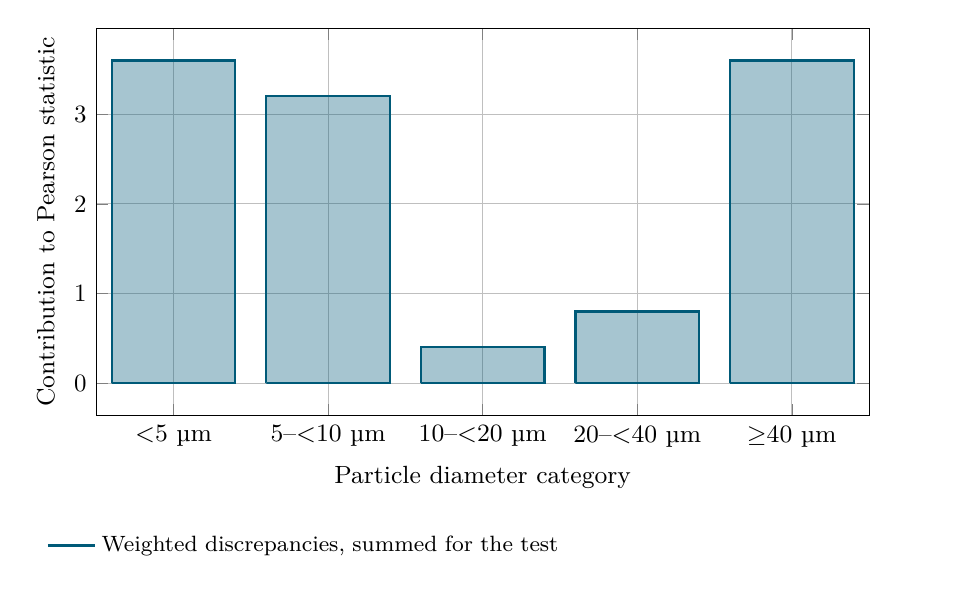
\begin{tikzpicture}
\begin{axis}[width=0.94\linewidth,
height=6.5cm,
scale only axis=false,
grid=major,
tick label style={font=\small},
label style={font=\small},
xlabel={Particle diameter category},
ylabel={Contribution to Pearson statistic},
legend style={font=\footnotesize,draw=none,at={(0.5,-0.28)},anchor=north,legend columns=1,text width=0.85\linewidth,align=left},
unbounded coords=jump,
scaled ticks=false,
xmin=0.5,
xmax=5.5,
xtick={1,2,3,4,5},
xticklabels={{<5 µm},{5–<10 µm},{10–<20 µm},{20–<40 µm},{\ensuremath{\ge}40 µm}}]
\addplot[color=pcd1,thick,fill=pcd1,fill opacity=0.35,mark=none] coordinates {(0.6,0) (0.6,3.6) (1.4,3.6) (1.4,0)} \closedcycle;
\addplot[color=pcd1,thick,fill=pcd1,fill opacity=0.35,forget plot,mark=none] coordinates {(1.6,0) (1.6,3.2) (2.4,3.2) (2.4,0)} \closedcycle;
\addplot[color=pcd1,thick,fill=pcd1,fill opacity=0.35,forget plot,mark=none] coordinates {(2.6,0) (2.6,0.4) (3.4,0.4) (3.4,0)} \closedcycle;
\addplot[color=pcd1,thick,fill=pcd1,fill opacity=0.35,forget plot,mark=none] coordinates {(3.6,0) (3.6,0.8) (4.4,0.8) (4.4,0)} \closedcycle;
\addplot[color=pcd1,thick,fill=pcd1,fill opacity=0.35,forget plot,mark=none] coordinates {(4.6,0) (4.6,3.6) (5.4,3.6) (5.4,0)} \closedcycle;
\addlegendentry{Weighted discrepancies, summed for the test}

\end{axis}
\end{tikzpicture}
\end{center}

% Full-precision experiment details: {"blockId":"ex:p1-n63-v--block","parameters":[{"key":"mode","label":"Count outcome: 0 departing, 1 compatible","value":0},{"key":"view","label":"Authored comparison / transformation view","value":1}],"readouts":[{"label":"Pearson statistic","value":11.600000000000001},{"label":"Degrees of freedom","value":4},{"label":"Upper-tail reference p","value":0.020587372268555525},{"label":"Prespecified upper 5% cutoff","value":9.48772903678115},{"label":"Decision","value":"Reject the stated proportions"},{"label":"Interpretation","value":"Counts differ significantly from stated proportions (5% level)"},{"label":"<5 µm contribution","value":3.6},{"label":"5–<10 µm contribution","value":3.2},{"label":"10–<20 µm contribution","value":0.4},{"label":"20–<40 µm contribution","value":0.8},{"label":"≥40 µm contribution","value":3.6}],"note":"Independent classifications, fixed exhaustive categories, fully specified probabilities and adequate expected counts supply the chi-square approximation for this grouped model check.","markers":[[]]}

\medskip

\par\medskip
\Needspace{8\baselineskip}
\refstepcounter{listing}\label{material-cdef5f2c042b23696f1df08f9b838e9ce625e4d658fcb9727eb2b6a16cde9590}
\noindent\textbf{Listing~\ref*{material-cdef5f2c042b23696f1df08f9b838e9ce625e4d658fcb9727eb2b6a16cde9590}.} R reproduction of the fixed-model Kolmogorov-Smirnov checks.\par\nopagebreak
\begin{Verbatim}[fontsize=\footnotesize,breaklines=true,breakanywhere=true]
n <- 5; a <- 0.05  # sample size; upper-tail level
tail <- function(d) { k <- 0:floor(n*(1-d))
  2*d*sum(choose(n,k)*(d+k/n)^(k-1)*(1-d-k/n)^(n-k)) }
uniroot(function(d) tail(d)-a, c(.500001,.999999), tol=1e-12)$root
# 0.5632751984. Exact shortcut here requires d above 0.5.
\end{Verbatim}

\medskip

\par\medskip
\Needspace{8\baselineskip}
\refstepcounter{listing}\label{material-007da72e9b6a7780c813e58674e90ac521983c7081c92ee07885e818070c4a03}
\noindent\textbf{Listing~\ref*{material-007da72e9b6a7780c813e58674e90ac521983c7081c92ee07885e818070c4a03}.} R reproduction of expected group counts and the Pearson decision.\par\nopagebreak
\begin{Verbatim}[fontsize=\footnotesize,breaklines=true,breakanywhere=true]
qchisq(1 - 0.05, df = 4)  # 9.487729
pchisq(11.6, df = 4, lower.tail = FALSE)  # 0.02058737
# Upper-tail 5% in the table = cumulative 95% for qchisq.
\end{Verbatim}

\medskip

Each assessment relates a particular observed pattern to the chosen model and testing conditions. Values beyond a calibrated cutoff provide evidence of incompatibility and guide investigation of the model, measurement context and data provenance. Values within that cutoff remain compatible with the model at the stated testing level. Together, the graphical and numerical views support an explicit assessment of how the proposed model describes variation.


\end{document}
